\documentclass[a4paper]{article}
    \usepackage[margin=0in]{geometry}
    \usepackage{multicol}
    \usepackage{graphicx}

    \begin{document}
    \begin{multicols}{3}
        \noindent\underline{\textbf{Week 1}}\\
        \textbf{Software testing}: process of executing program/system with intent of finding errors\\
        \textbf{Fault}: incorrect portions of code (can be missing as well as incorrect)\\
        \textbf{Failure}: observable correct behaviour of program\\
        \textbf{Error}: cause of fault, something bad programmer did (conceptual, typo, etc)\\
        \textbf{Bug}: informal term for fault\\
        \textbf{Test case}: set of test inputs, execution conditions, expected results developed for particular objective, such as to exercise particular program path ot verify compliance with specific requirement\\
        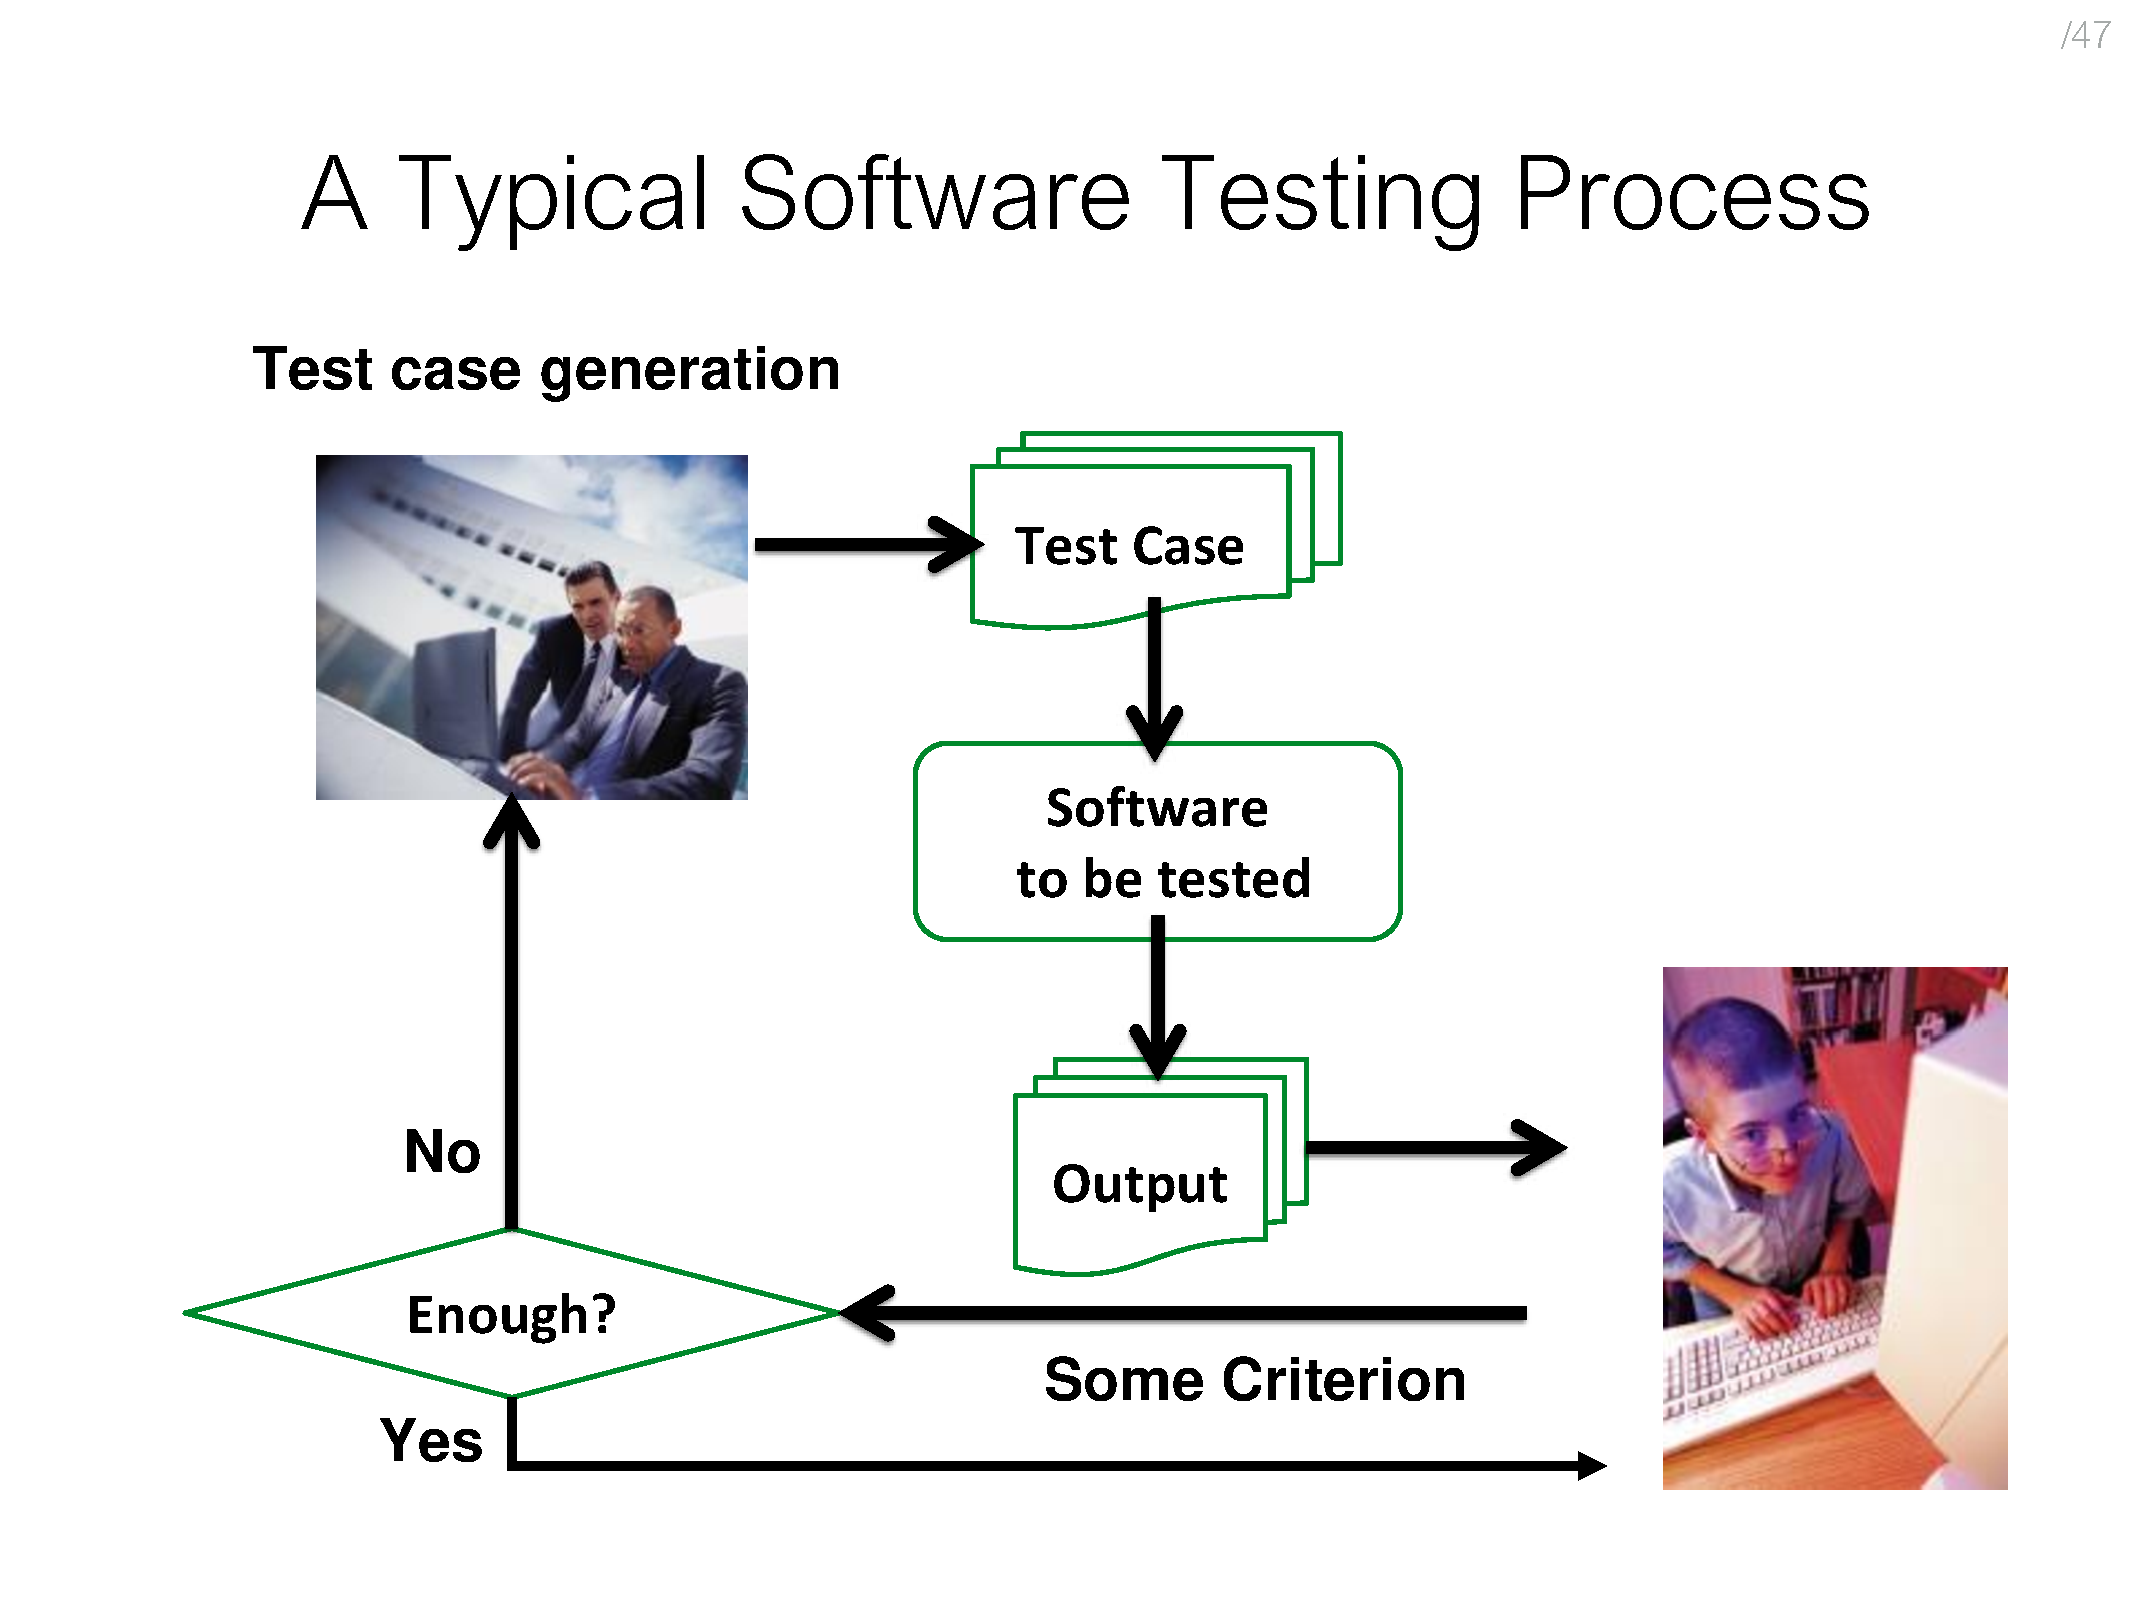
\includegraphics[width=\linewidth]{22.pdf}\\
        \textbf{Testing}: find inputs that cause failure of software, failure unknown, performed by testers\\
        \textbf{Debugging}: process of finding \& fixing fault given failure, failure is known, performed by devs\\
        \textbf{Black-Box/Functional Testing}: identify functions \& design test cases to check whether functions are correctly performed by software (formal \& informal specs)\\
        \textbf{Equivalence partitioning}: divide into partitions, select 1 test case from each partition, partitions must be disjointed (no input belongs to more than 1 partition) \& all partitions must cover entire input domain\\
        \textbf{Equivalence partitioning examples}: isEven then even \& odd, password min 8 \& max 12 characters then less than, valid, more than\\
        \textbf{\textbf{Boundary-Value analysis}}: partition input domain, identify boundaries, select test data (for range $[R_1,R_2]$ less than $R_1$, equal to $R_1$, between, equal to $R_2$, greater than $R_2$, for unordered sets select in \& not in, for equality select equal \& not equal, for sets, lists select empty \& not empty)\\
        \textbf{White box/structural testing}: generate test cases based on program structure, abstract program to control flow graph (node is sequence of statements, edge is transfers of control)\\
        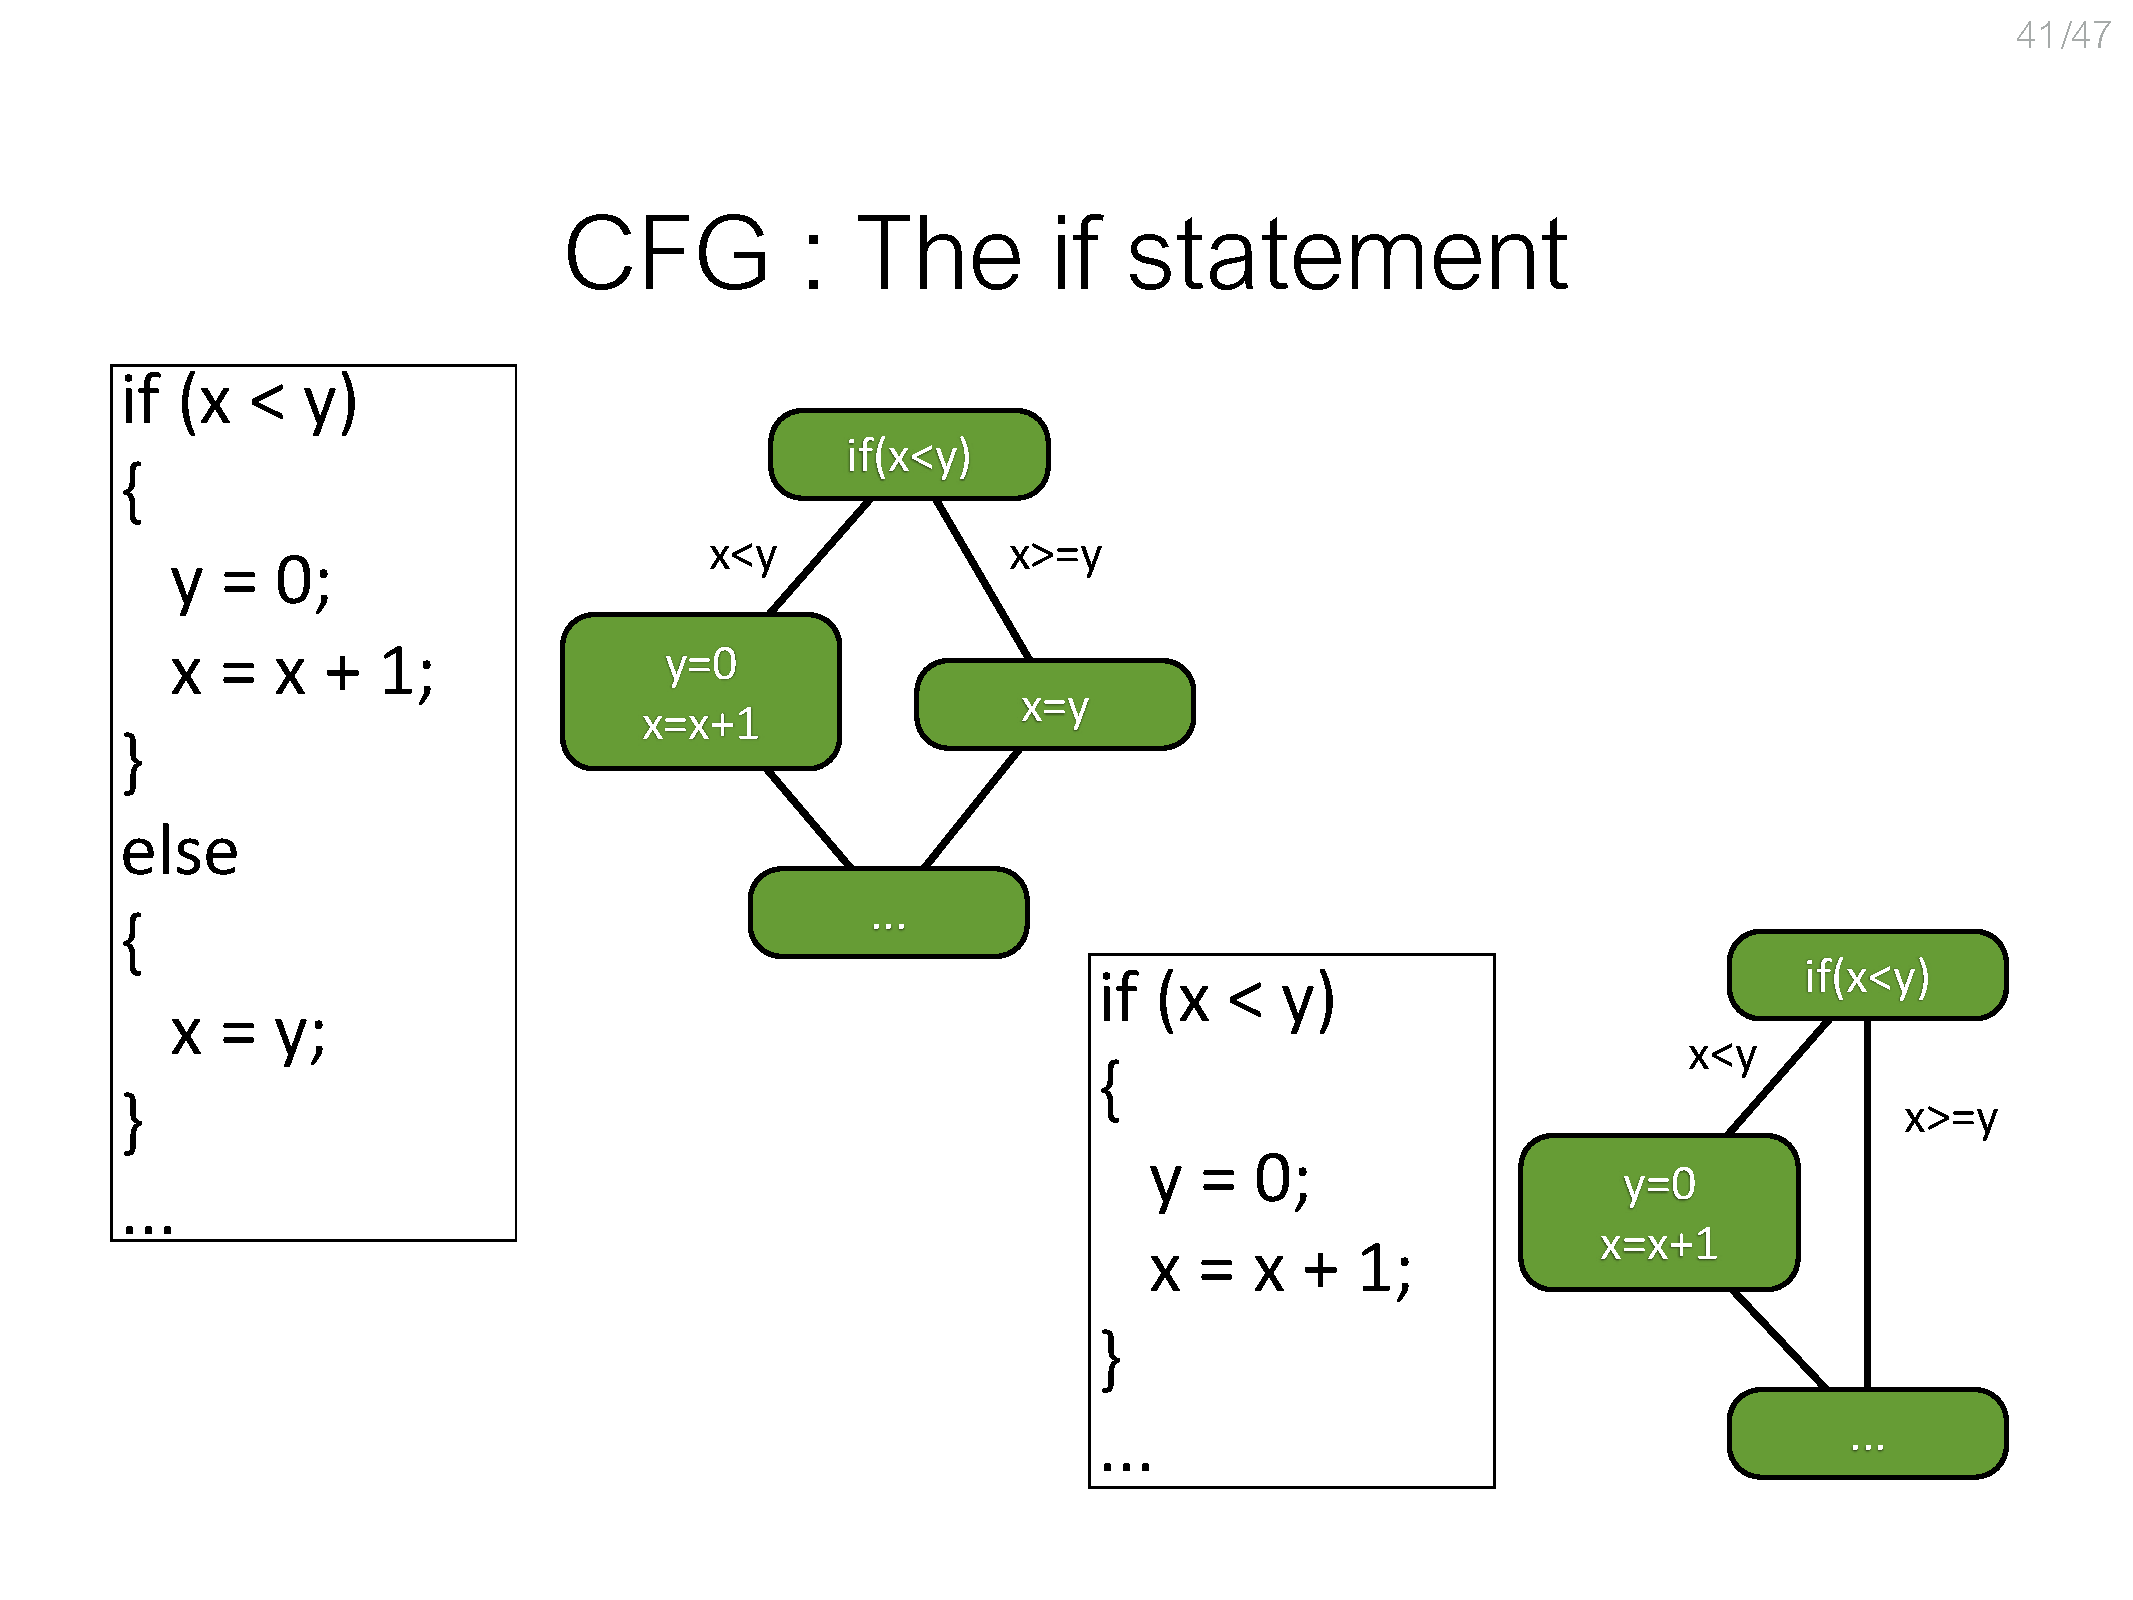
\includegraphics[width=\linewidth]{41.pdf}\\
        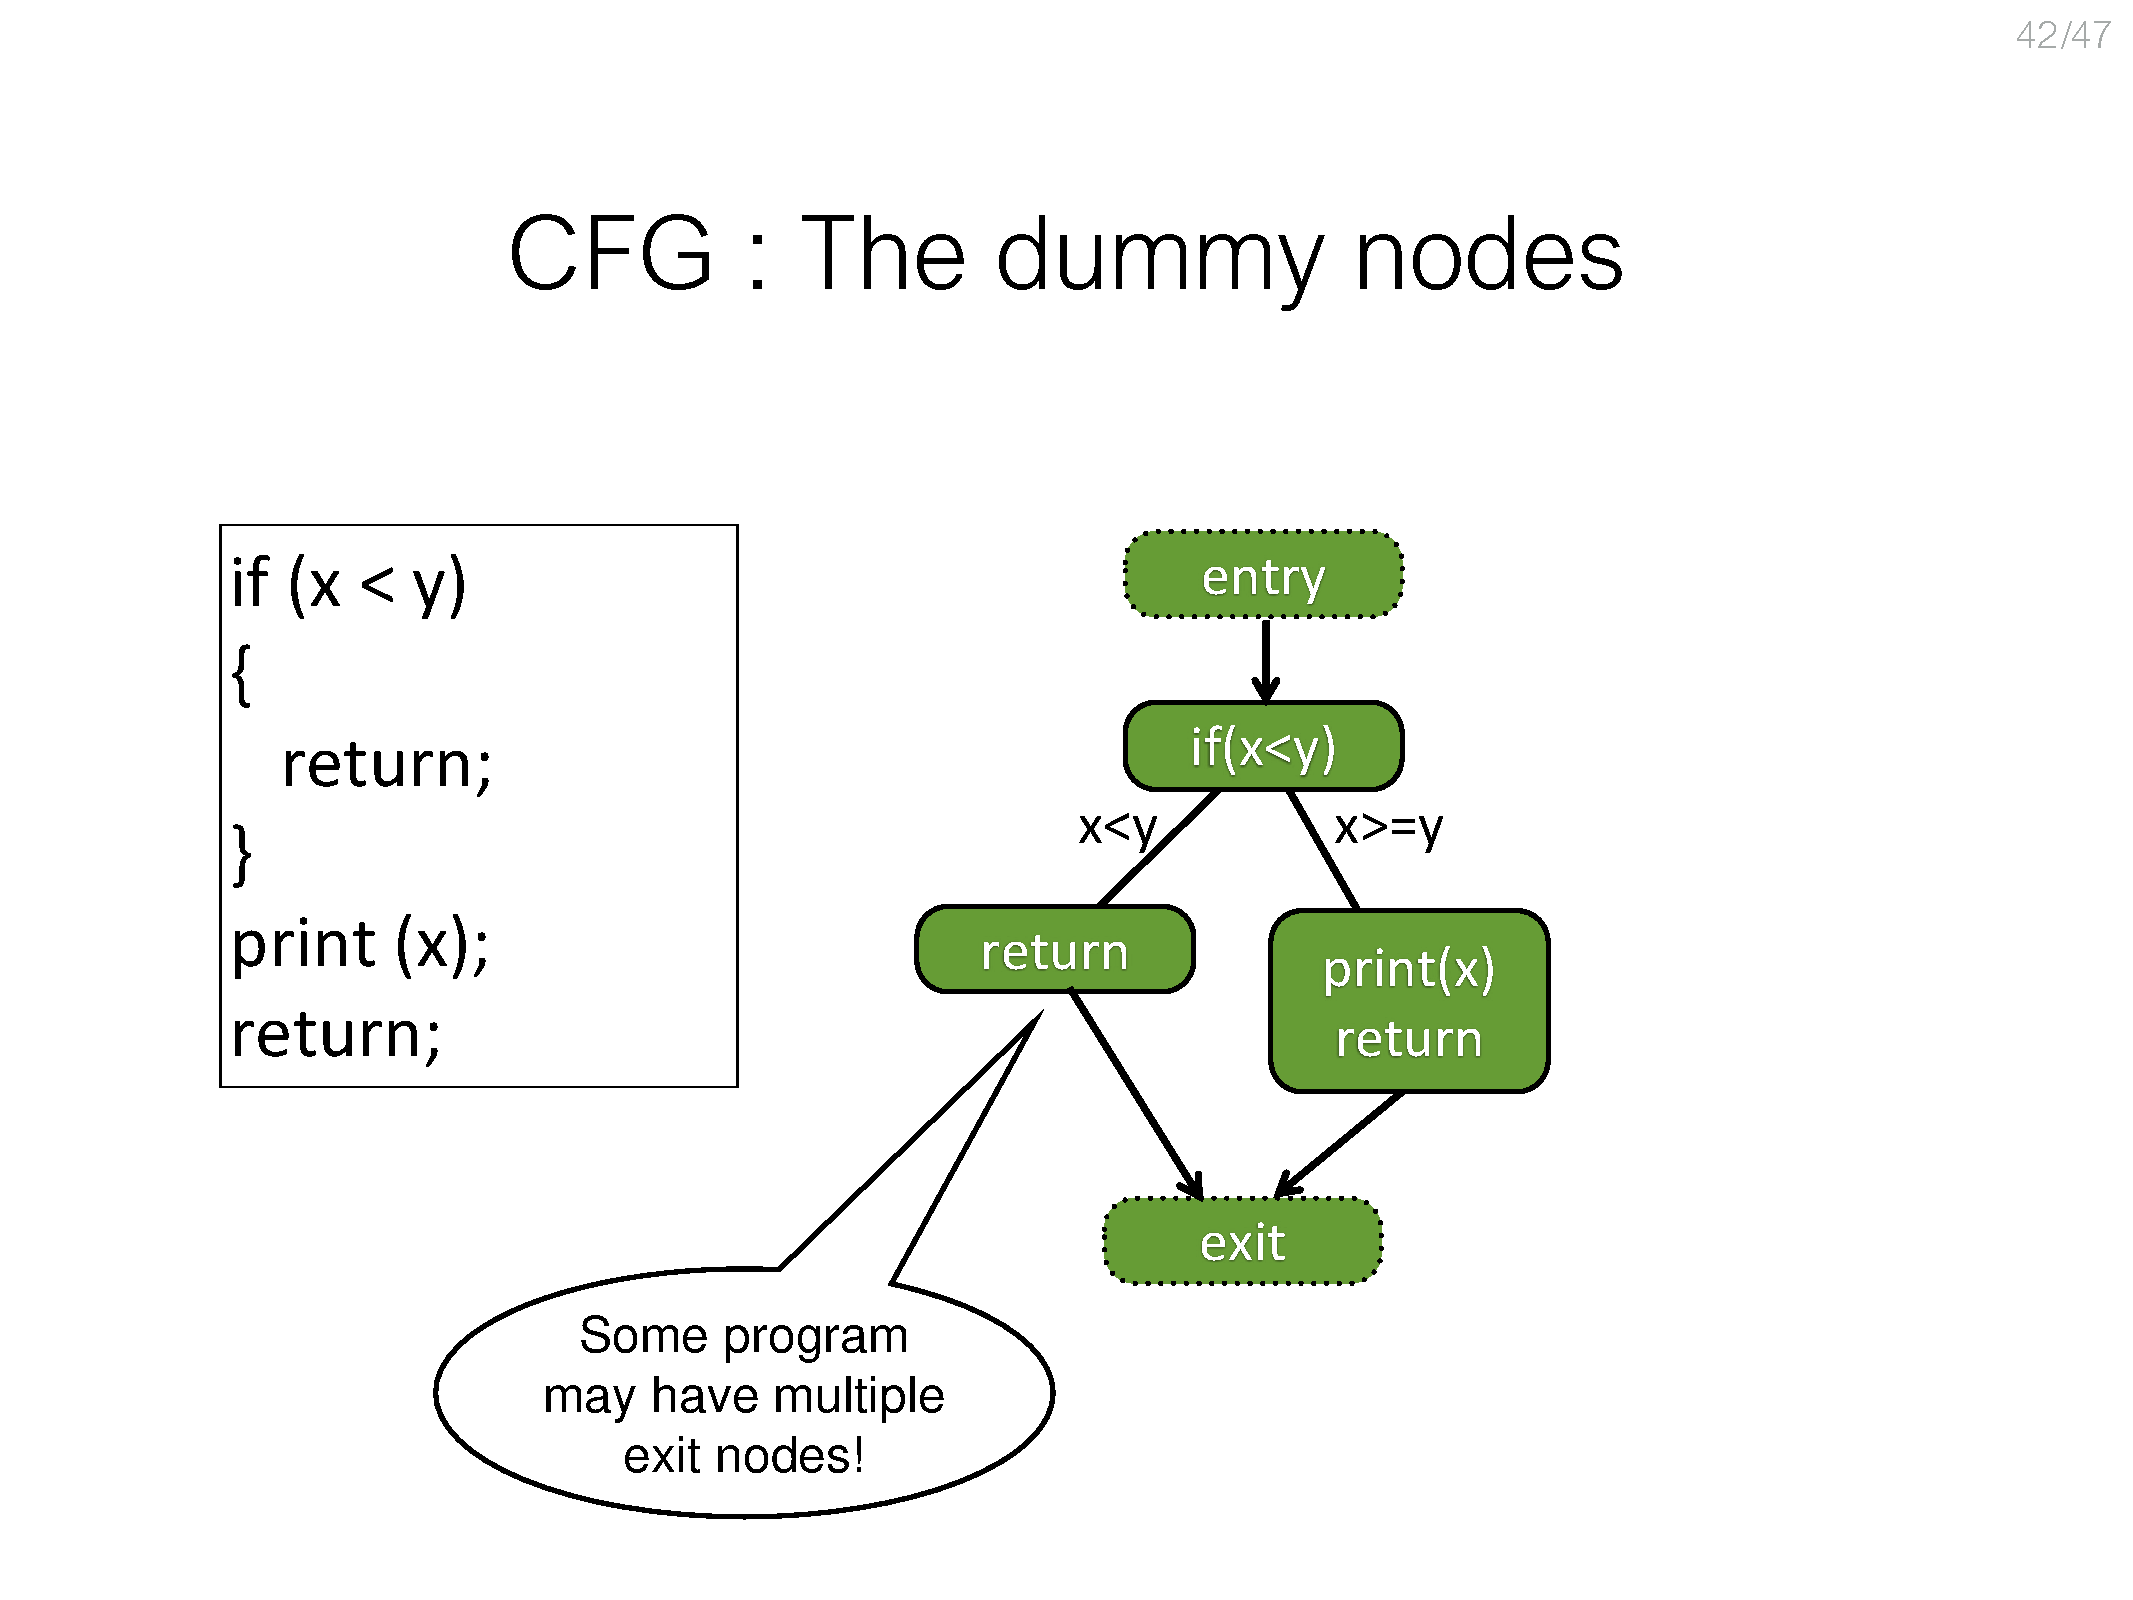
\includegraphics[width=\linewidth]{42.pdf}\\
        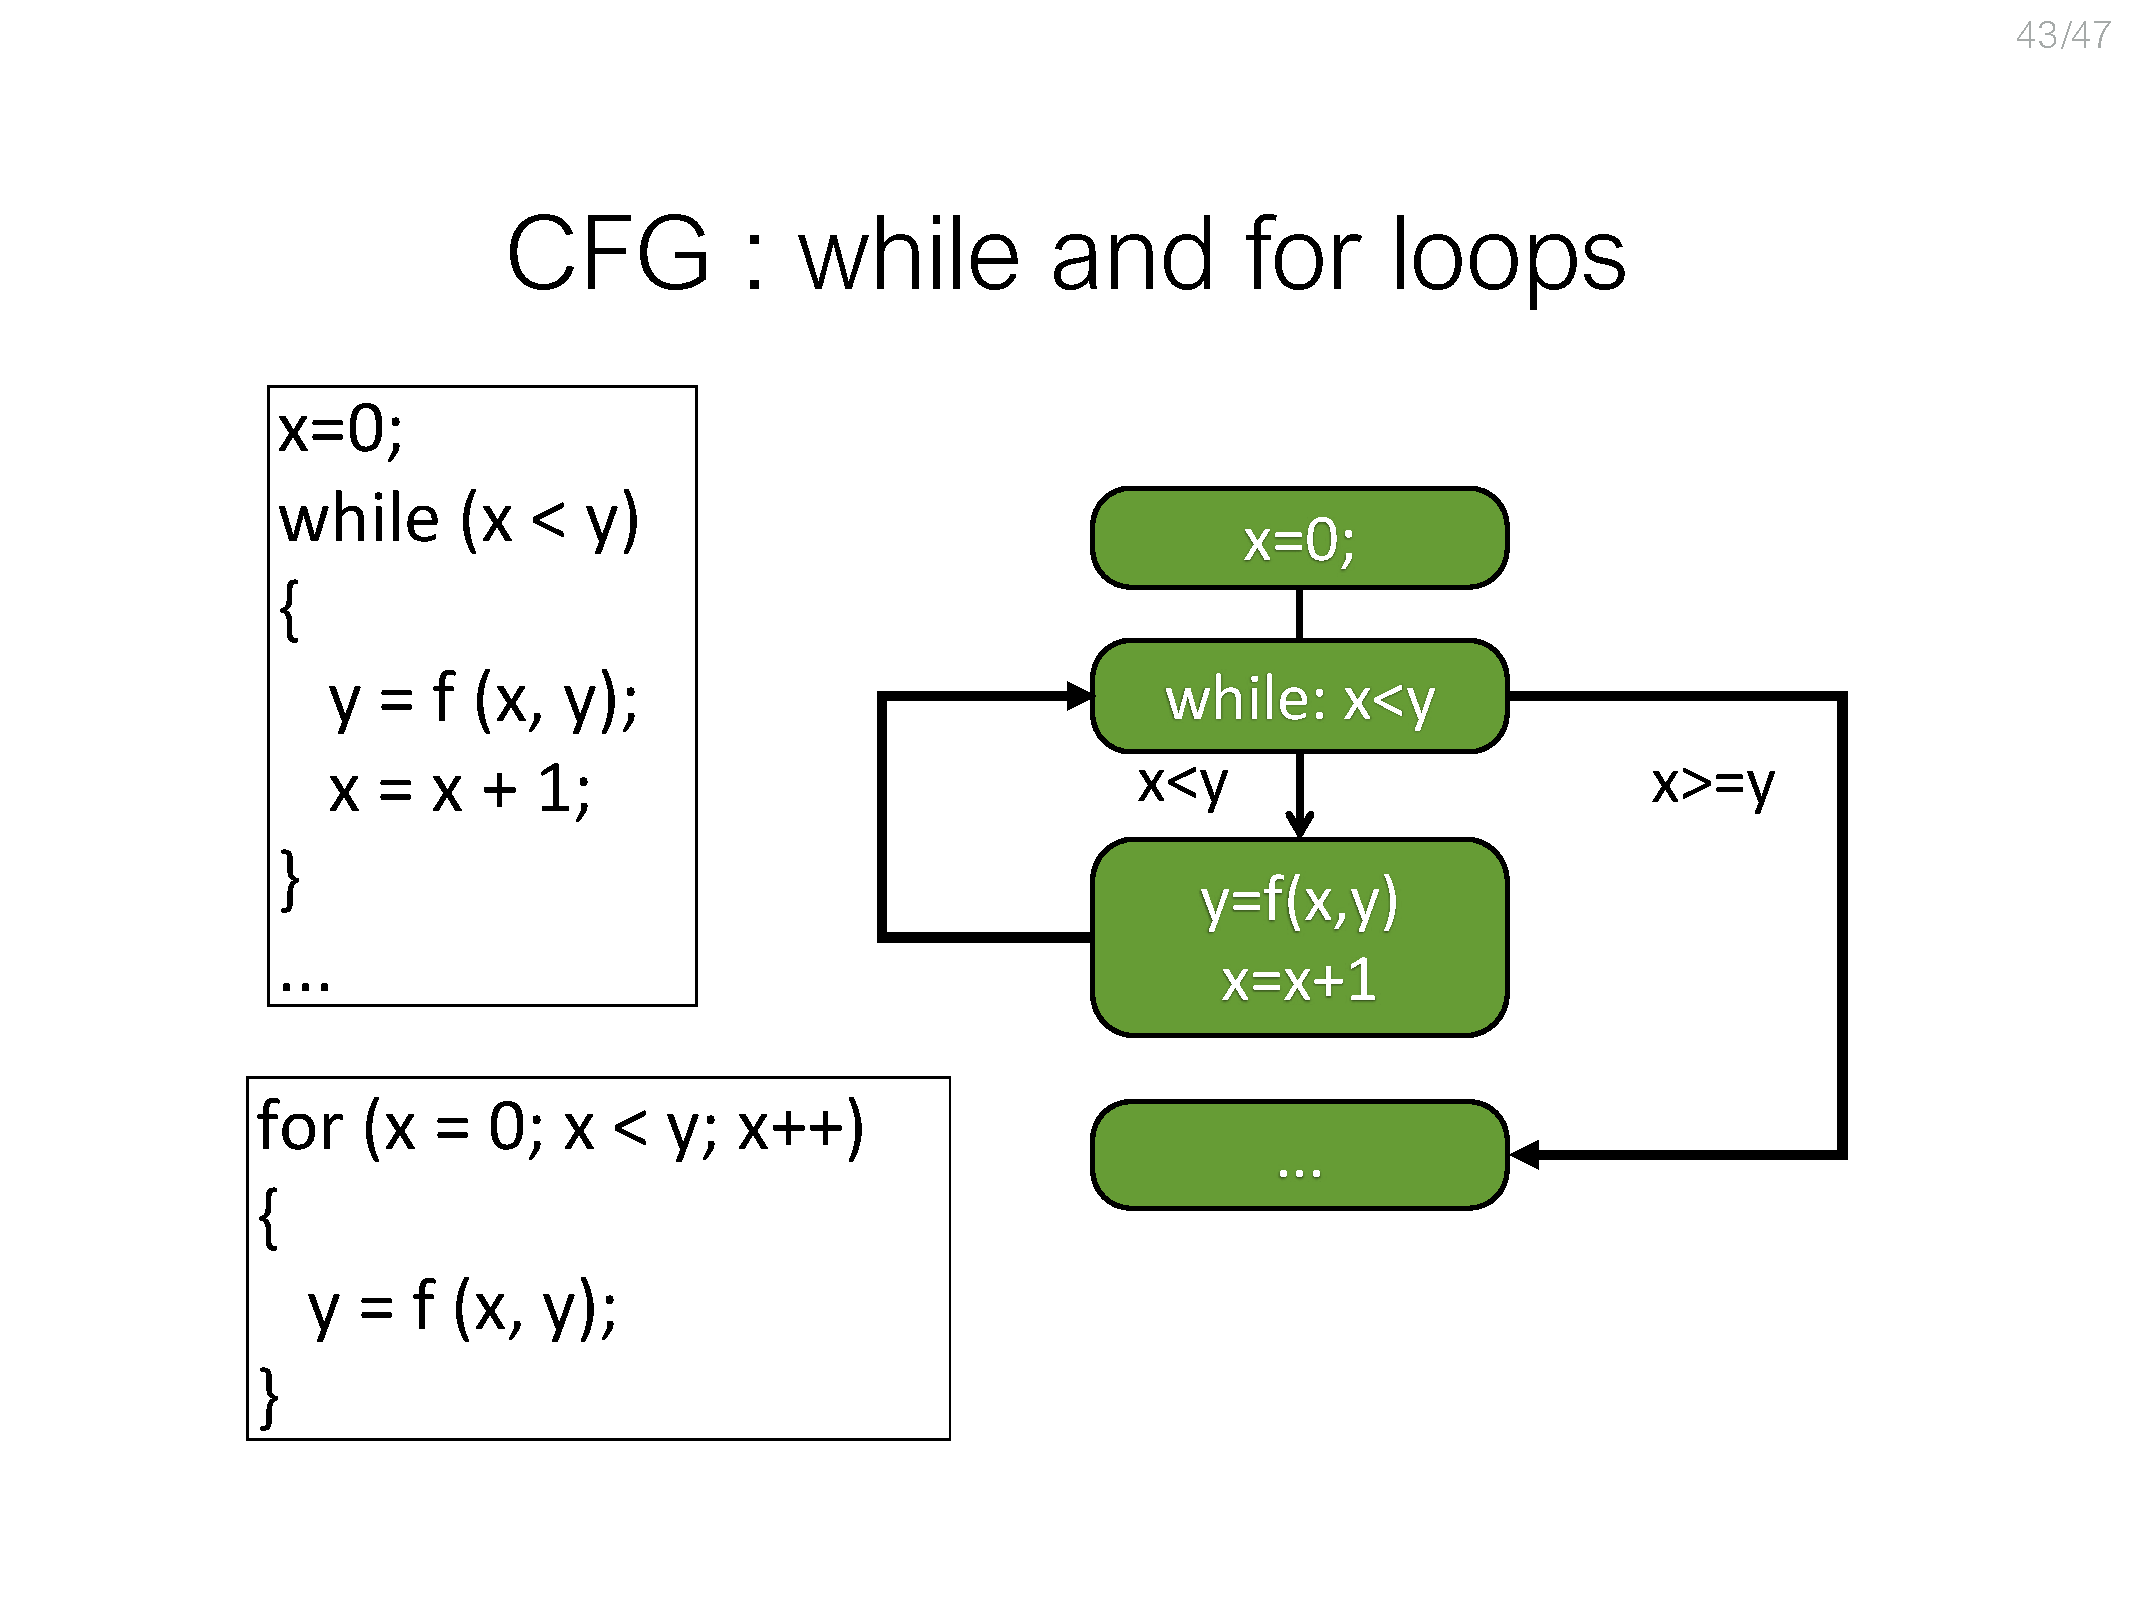
\includegraphics[width=\linewidth]{43.pdf}\\
        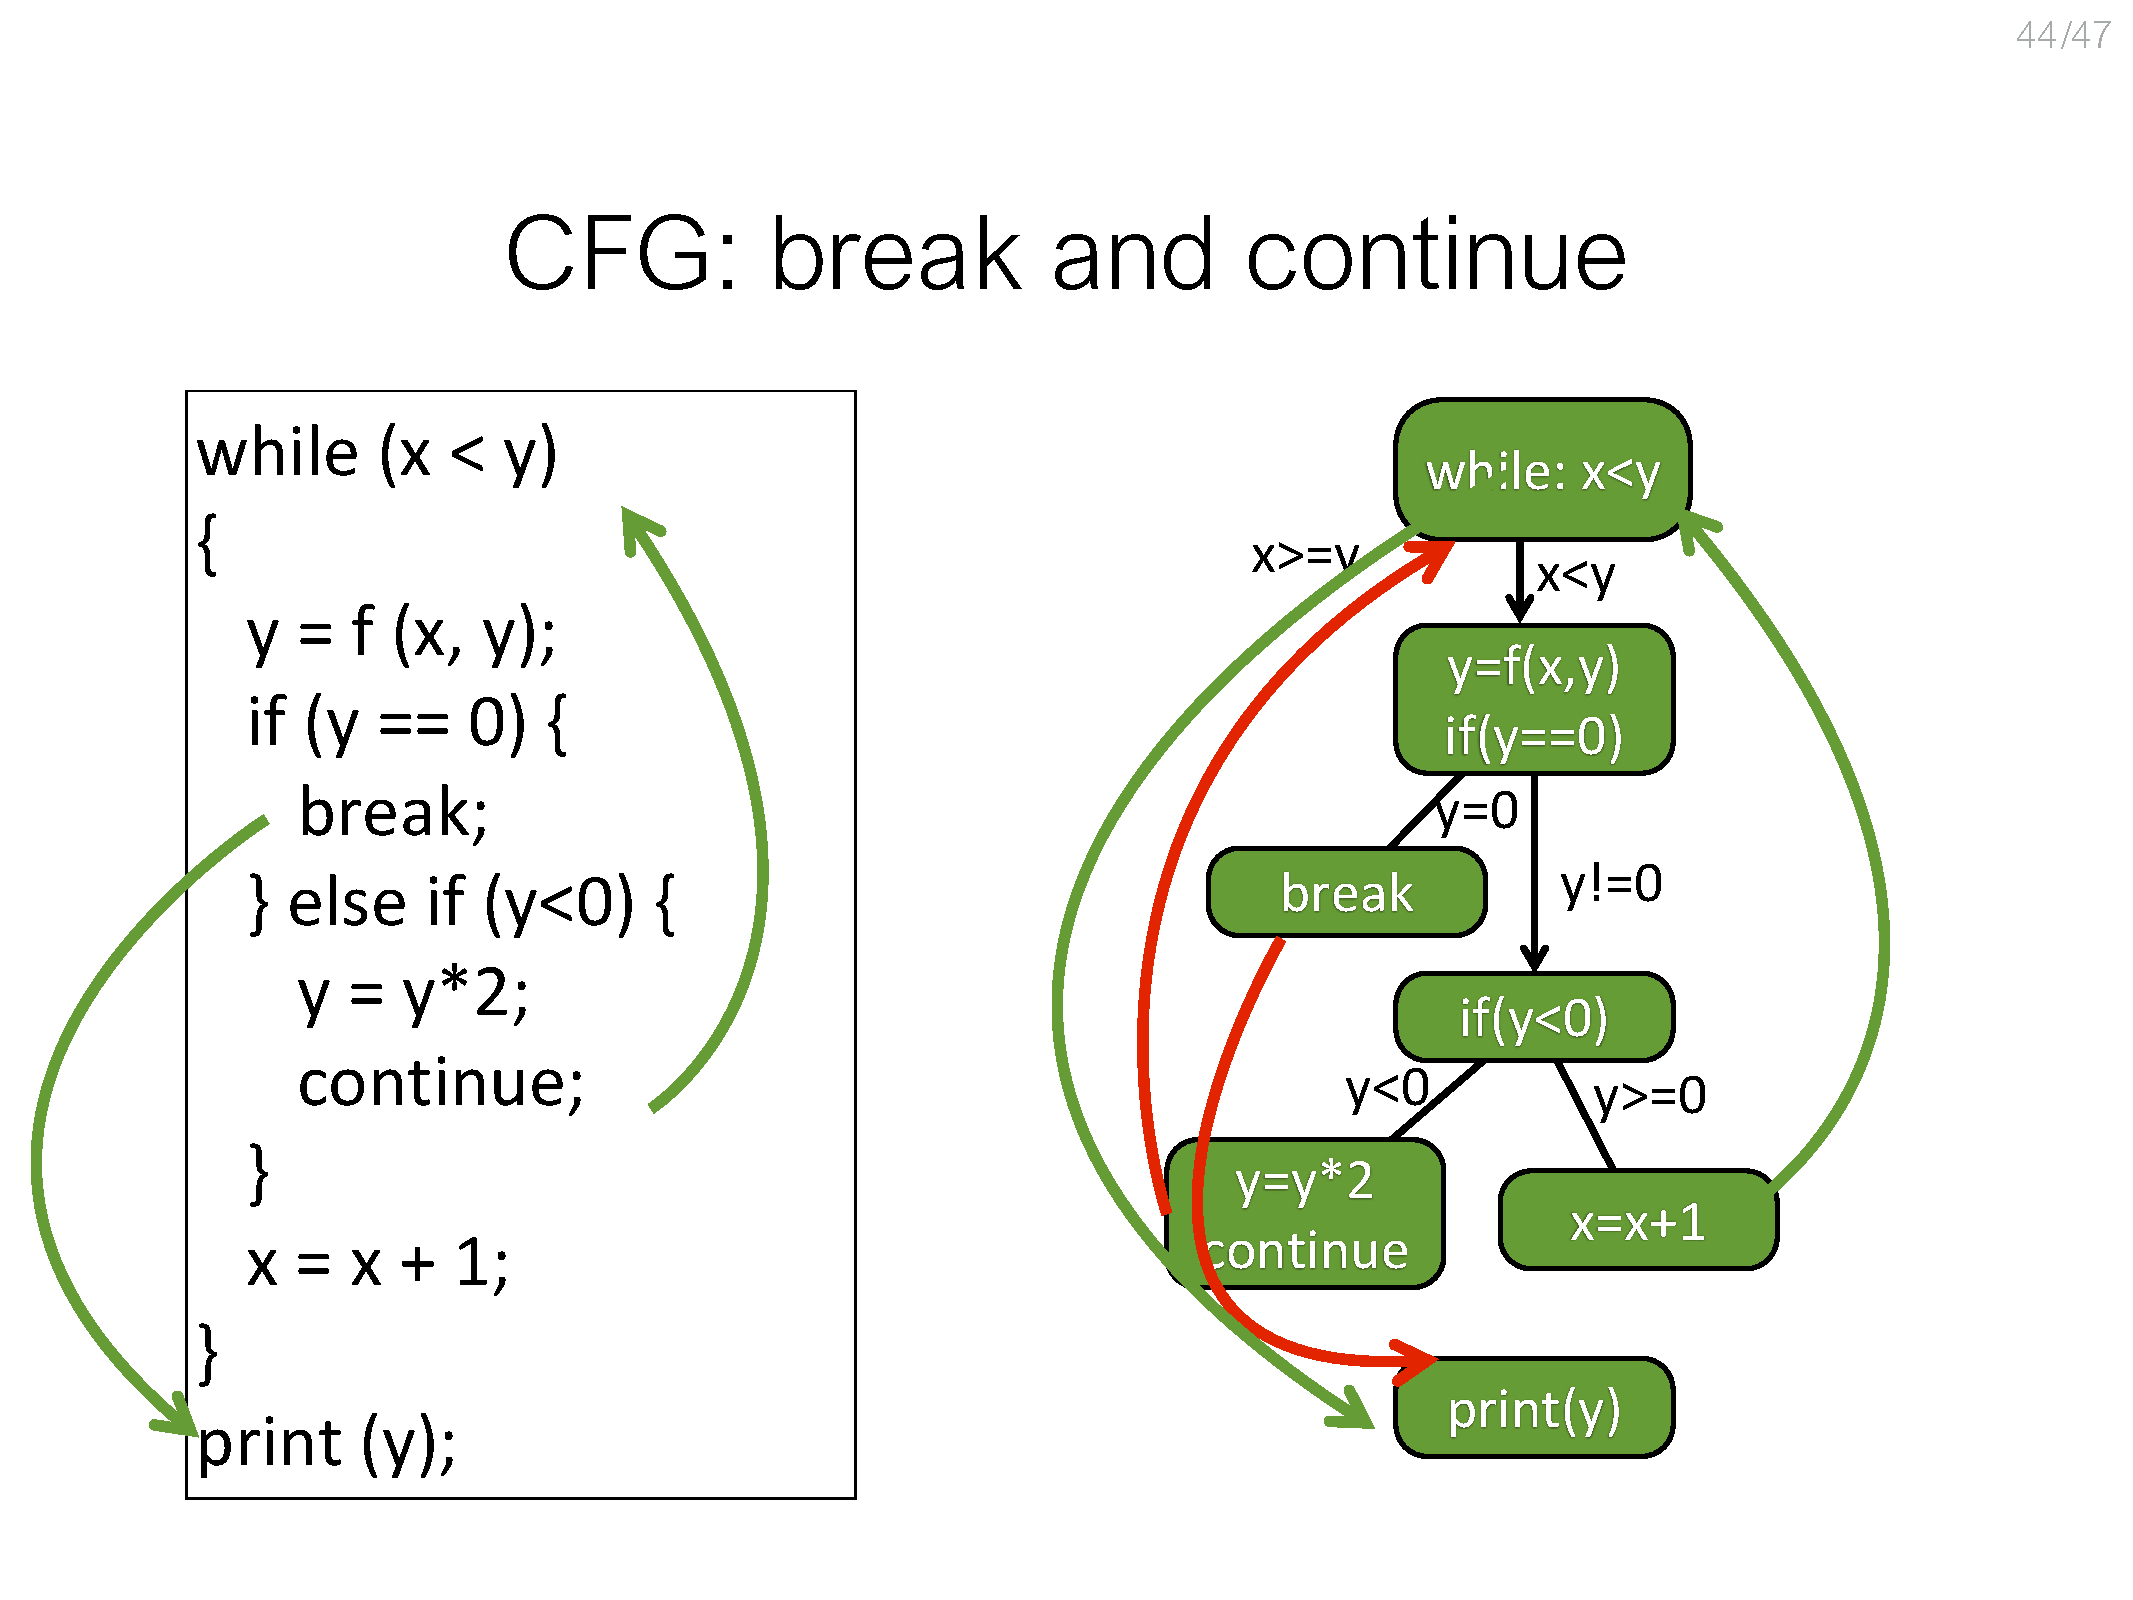
\includegraphics[width=\linewidth]{44.pdf}\\
        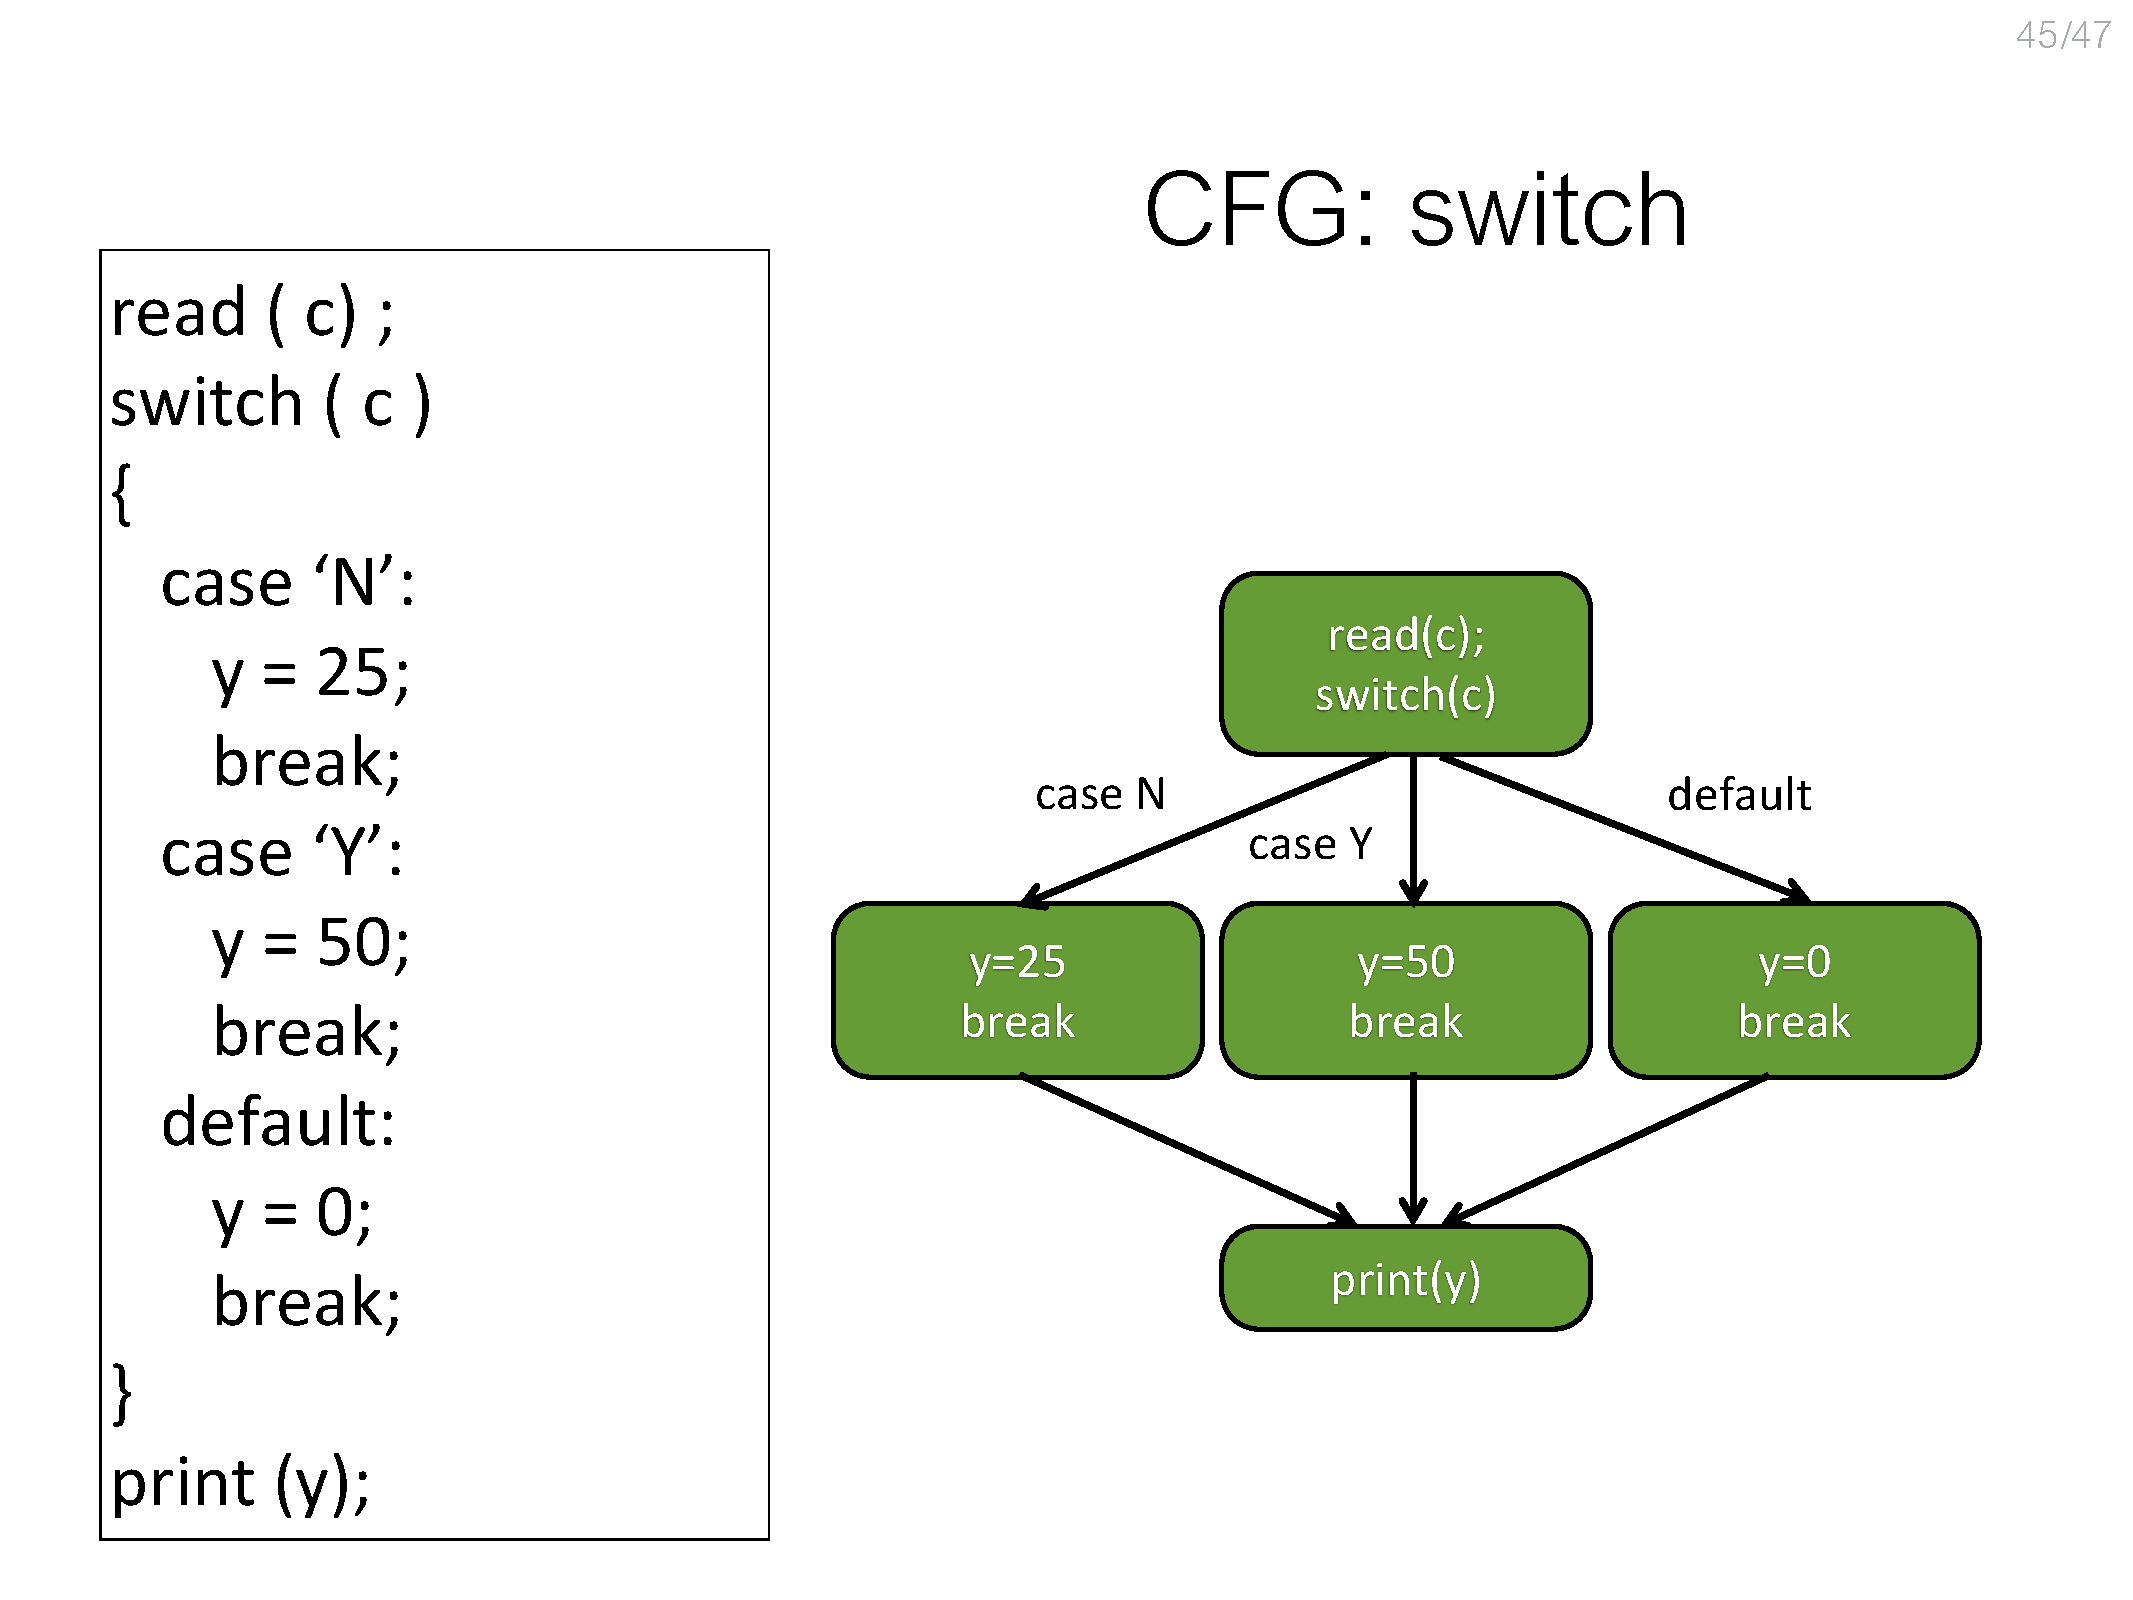
\includegraphics[width=\linewidth]{45.pdf}\\
        \textbf{Coverage types}: statement, branch, path (infinite if loop exists), strictly subsumes all beforehand\\
        \vfill\null\columnbreak\noindent\underline{\textbf{Week 2}}\\
        \textbf{Test oracle}: expected output of software for given input, part of test case\\
        \textbf{Test driver}: software framework that can load collection of test cases or test suite\\
        \textbf{Test suite}: collection of test cases\\
        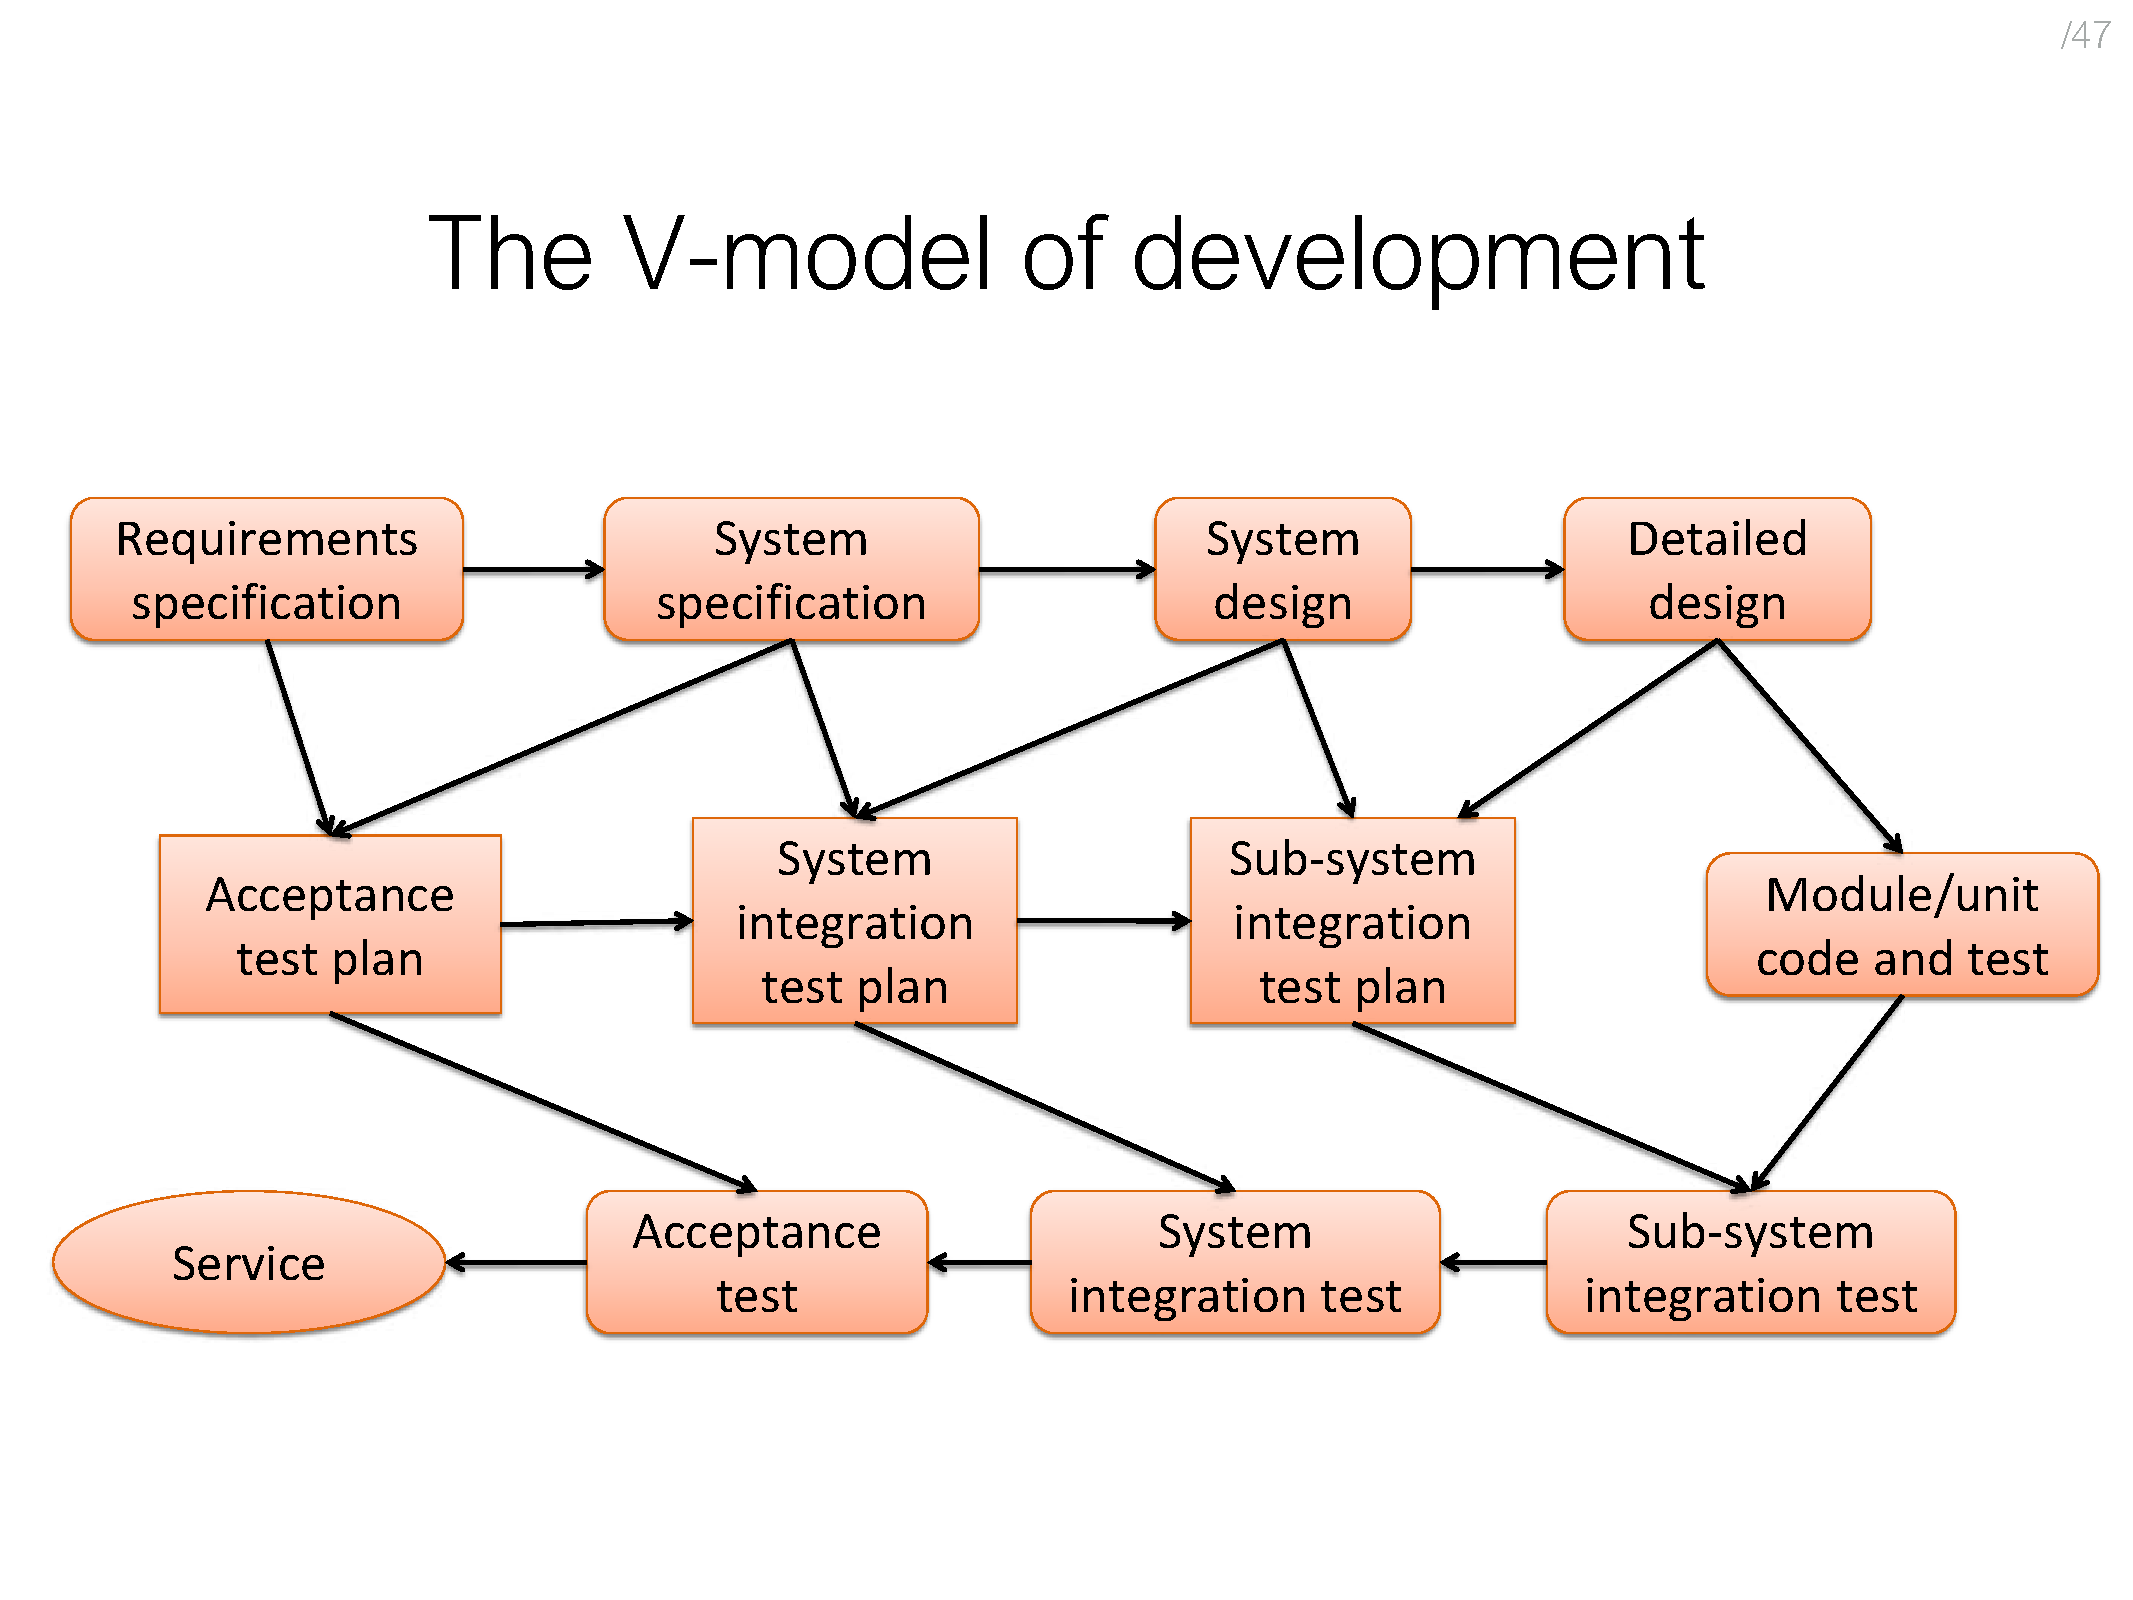
\includegraphics[width=\linewidth]{96.pdf}\\
        \textbf{Testing types}:\\
        \textit{Unit/Module}: test single module in isolated environment, use drivers \& stubs for isolation\\
        \textit{Integration}: test parts of system by combining modules, integrated collection of modules tested as group or partial system\\
        \textit{System}: test system as a whole after integration phase\\
        \textit{Acceptance}: test system as a whole to find out if it satisfies requirements specifications\\
        \textbf{Driver}: program that calls interface procedures of module being tested \& reports results, simulates module that calls module currently being tested, also provides access to global variables for module under test\\
        \textbf{Stub}: program that has same interface as module being used by module being tested but simpler, simulates module called by module being tested\\
        \textbf{Mock objects}: create object that mimics behaviour needed for testing\\
        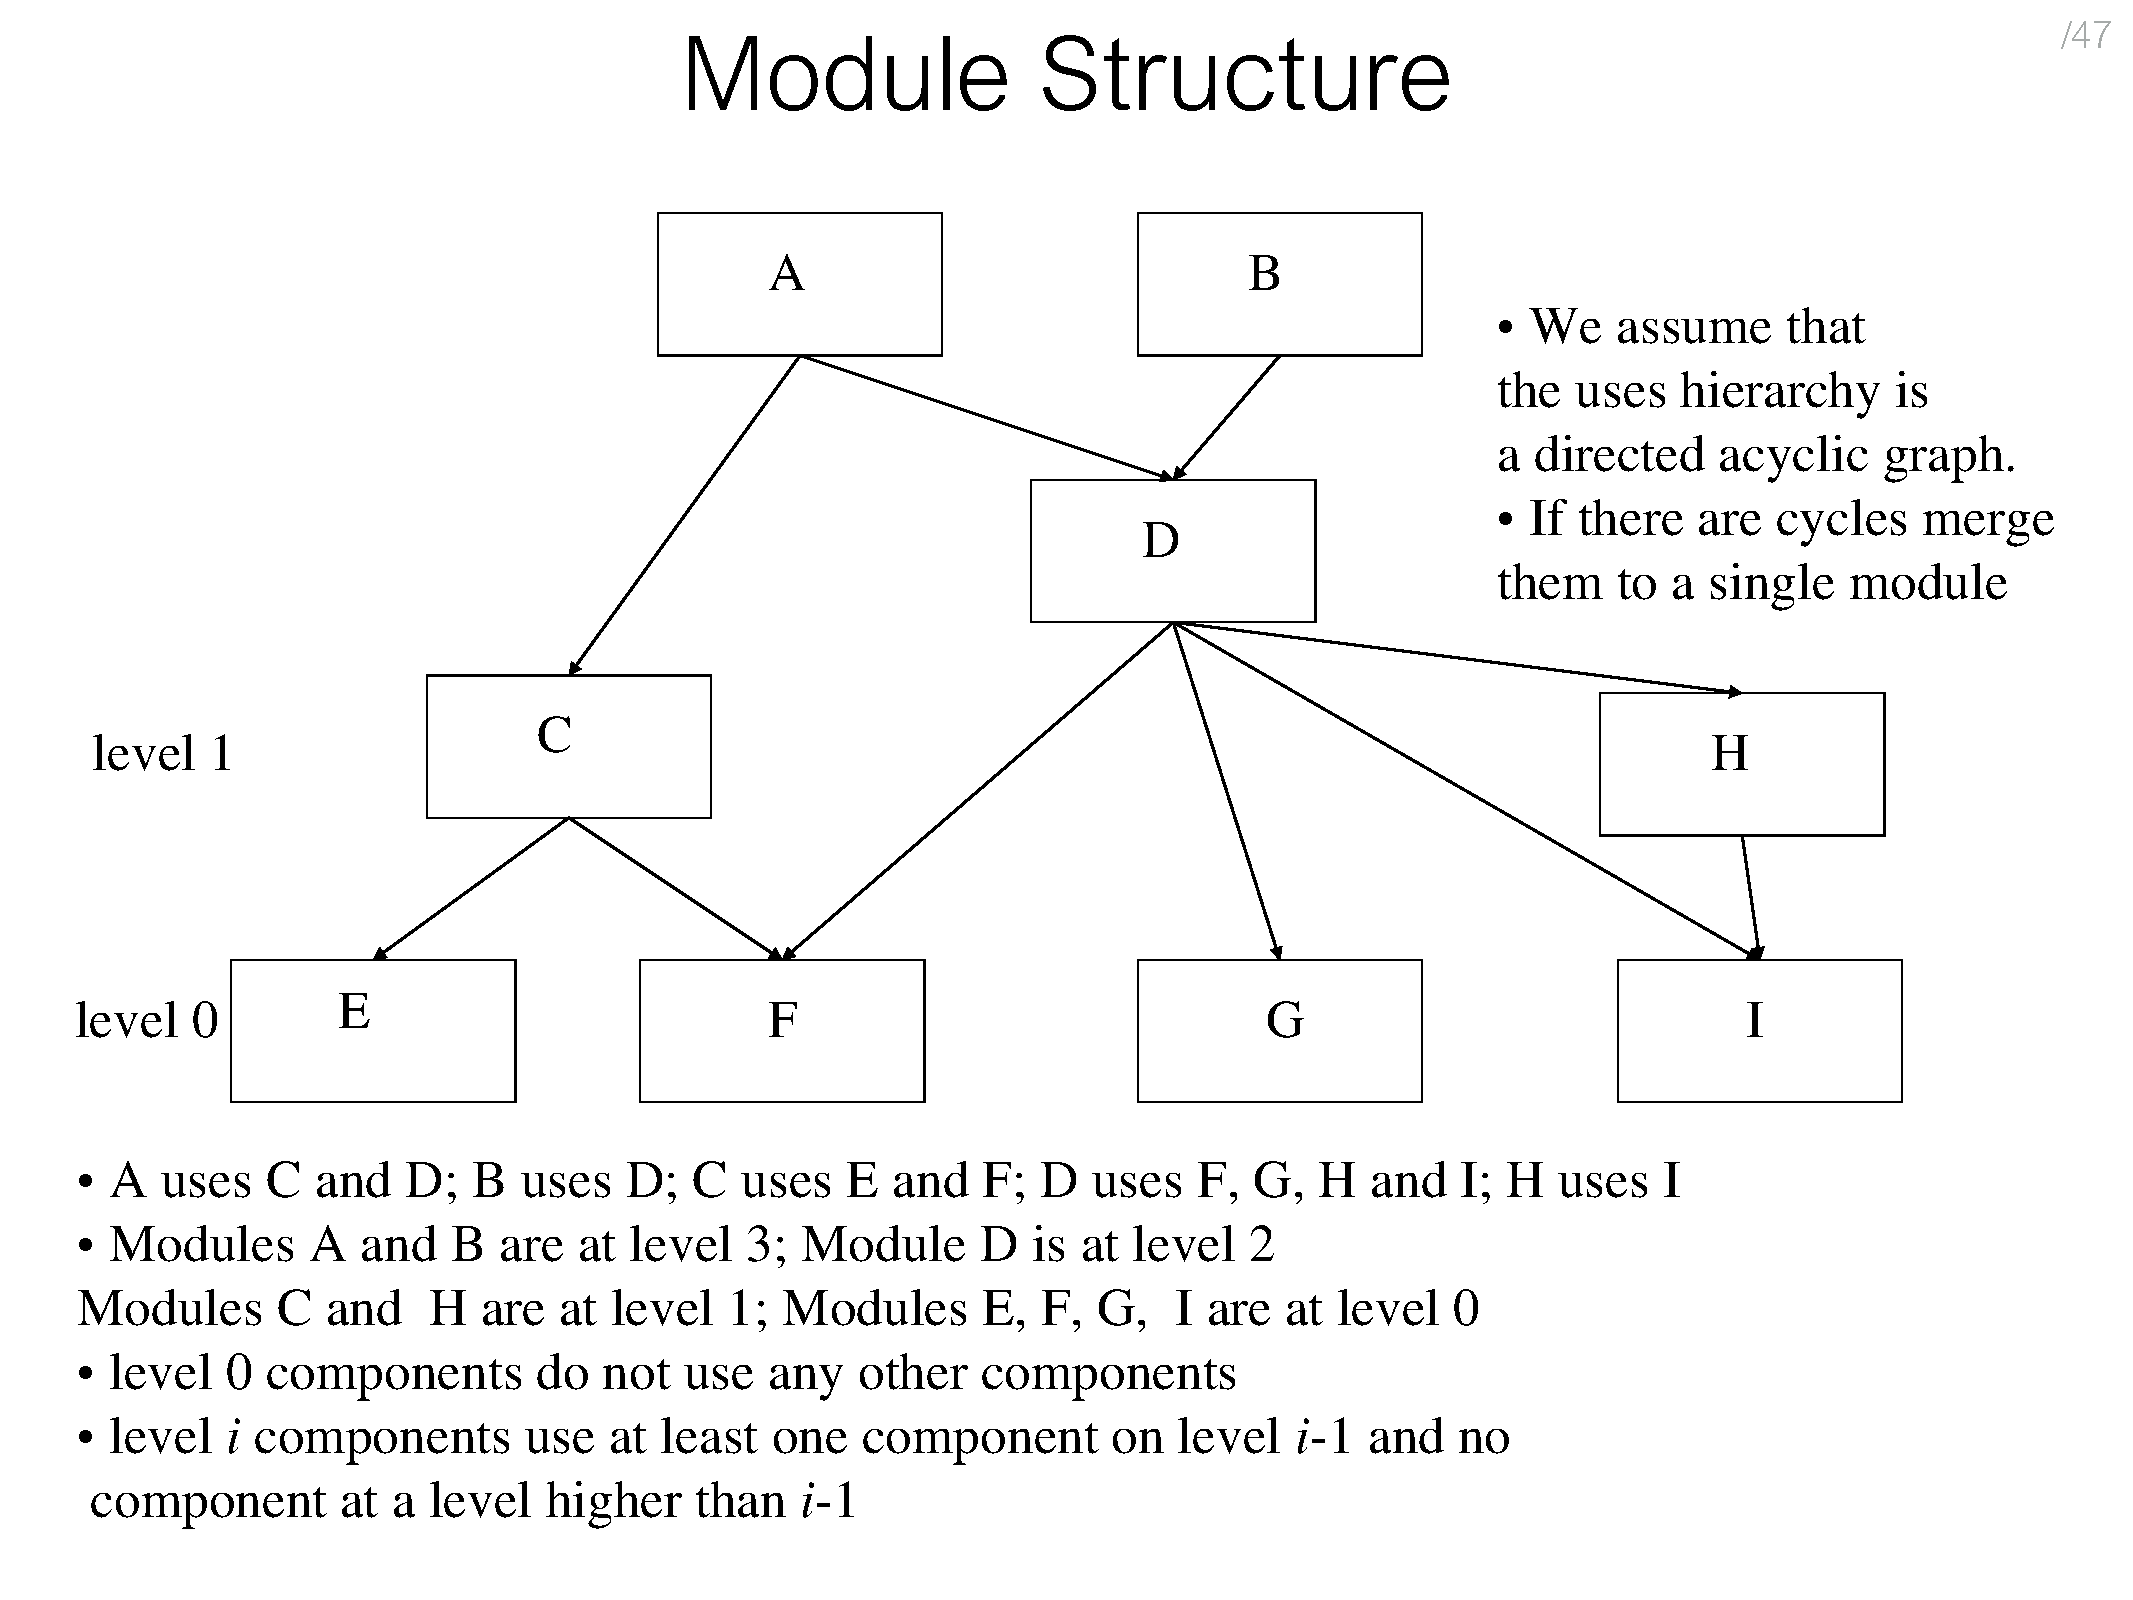
\includegraphics[width=\linewidth]{102.pdf}\\
        \textbf{Integration types}:\\
        \textit{Bottom-Up}: only terminal modules tested in isolation, requires drivers but not stubs (since lower levels are tested already)\\
        \textit{Top-down}: modules tested in isolation are modules at highest level, requires stubs but not drivers\\
        \textit{Sandwich}: begin both bottom-up \& top-down, meet at predetermined point in middle\\
        \textit{Big bang}: every module unit tested, then integrate all at once, no driver or stub needed but may be hard to isolate bugs\\
        \textbf{System/Acceptance testing}: can construct test case based on requirements specifications, main purpose is to assure that system meets requirements, alpha testing performed within development organisation, beta testing performed by select group of friendly customers\\
        \underline{\textbf{Week 3}}\\
        \textbf{Basis Path Testing}: between branch \& path coverage, fulfills branch testing \& tests all independent paths that could be used to construct any arbitrary path through computer program\\
        \textbf{Independent path}: includes some vertices/edges not covered in other path\\
        \textbf{Cyclomatic complexity}: $e-n+2p$, $e$ is edges, $n$ is nodes, $p$ is number of connected components, or $1+d$, $d$ is loops or decision points, upper bound on number of test cases to guarantee coverage of all statements\\
        \textbf{Decision Coverage}: executing true/false of decision\\
        \textbf{Condition Coverage}: executing true/false of each condition\\
        \textbf{Condition/Decision Coverage}: DC \& CC, better than either\\
        \textbf{Multiple Condition Coverage}: whether every possible combination of boolean sub-expressions occurs, test cases are truth table, $2^n$ test cases for $n$ conditions\\
        \textbf{Modified C/DC}: for each basic condition $C$, 2 test cases, values of all evaluated conditions except $C$ are the same, compound decision as a whle evaluates to true for 1 \& false for the other, subsumed by MCC \& subsumes CC, DC, C/DC, stronger than statement \& branch\\
        \textbf{MC/DC coverage}: each entry \& exit point invoked, each decision takes every possible outcome, each condition in a decision takes every possible outcome, each condition in decision is shown to independenly affect outcome of decision, independence of condition is shown by proving that only one condition changes at a time\\
        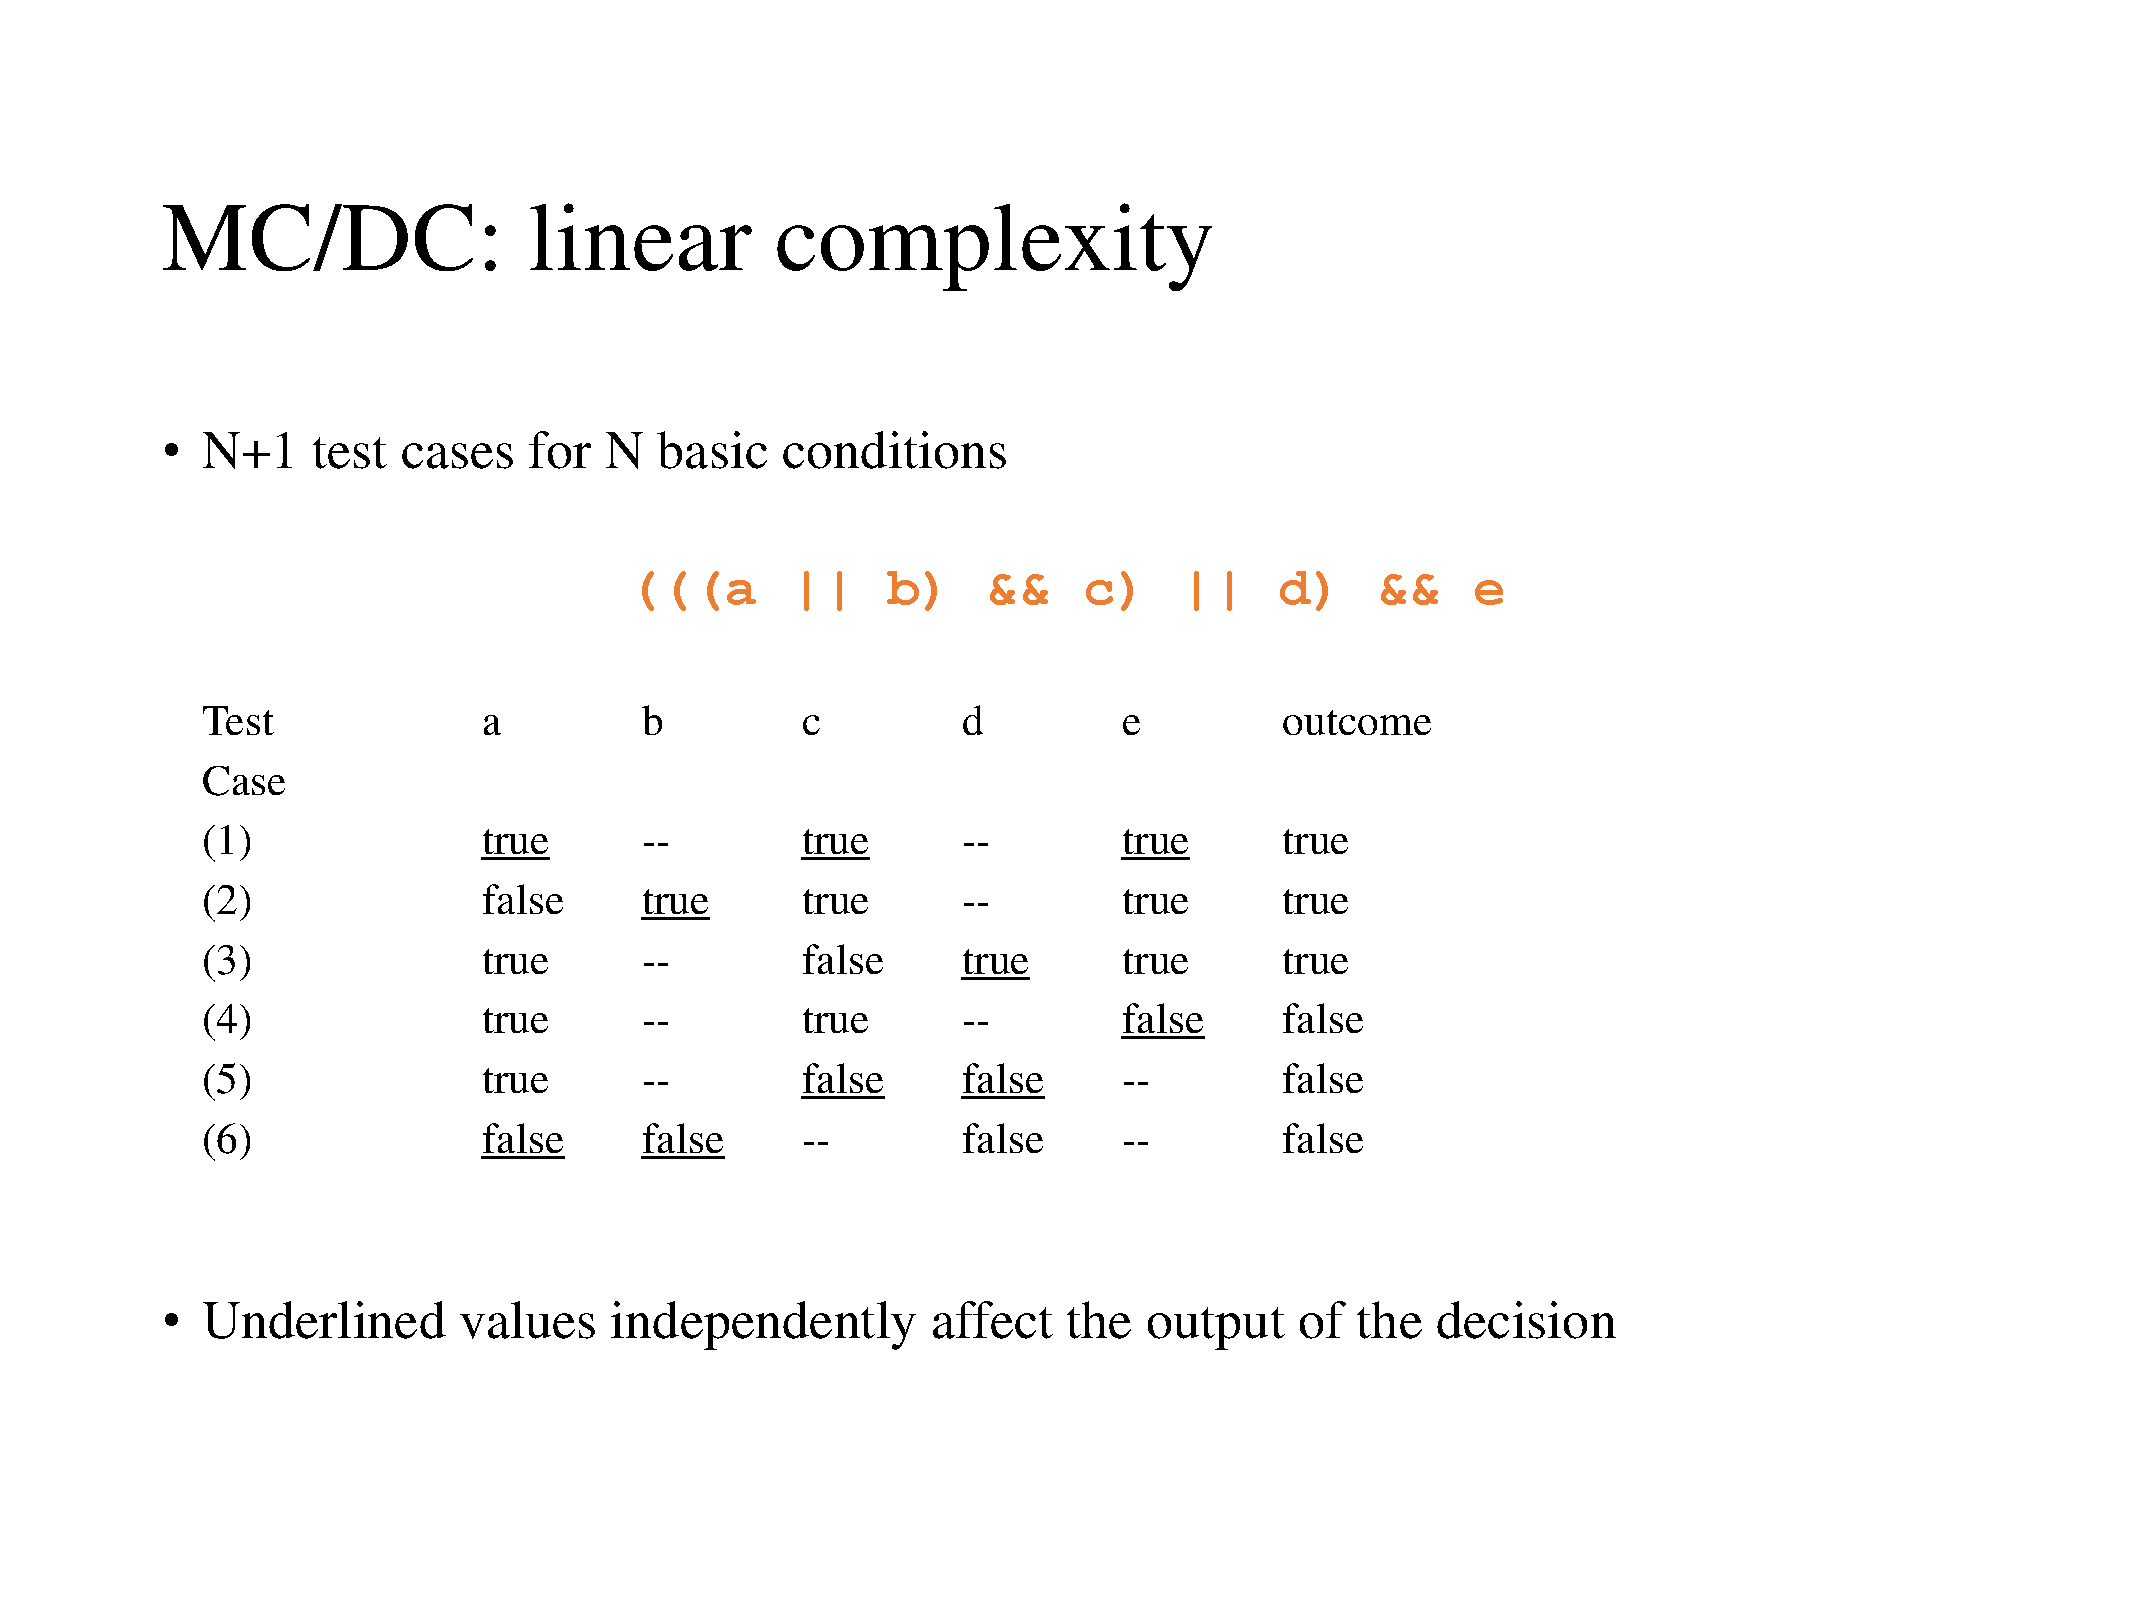
\includegraphics[width=\linewidth]{148.pdf}\\
        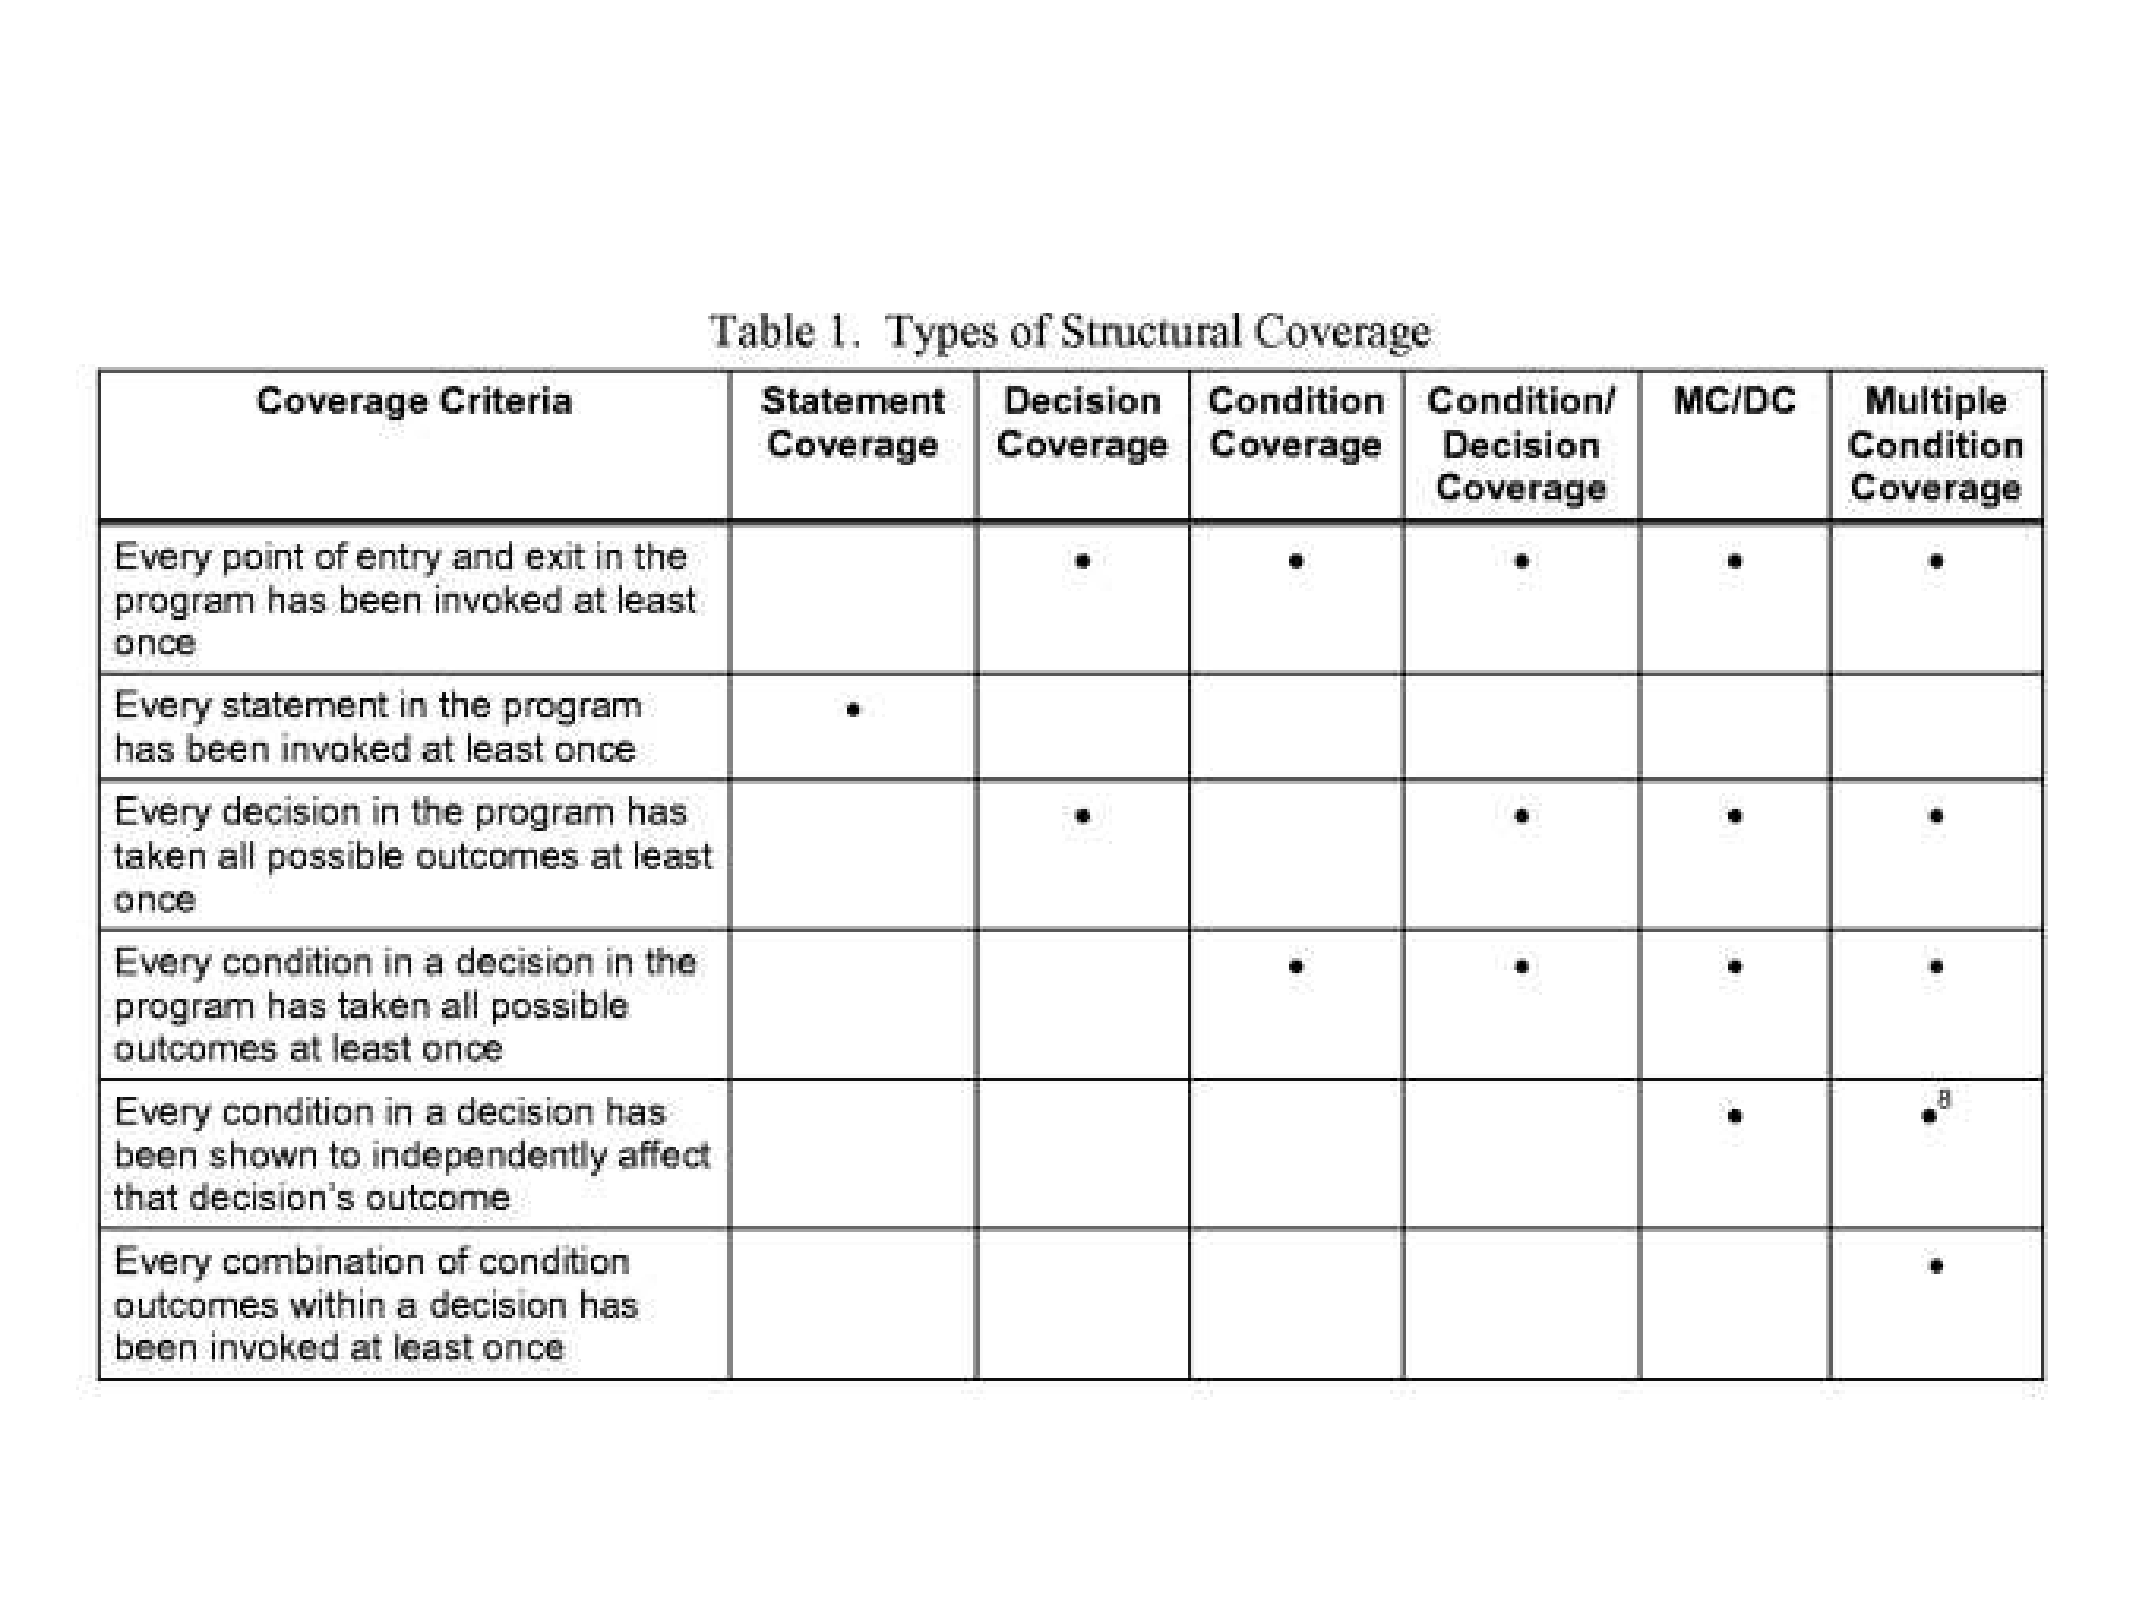
\includegraphics[width=\linewidth]{152.pdf}\\
        \vfill\null\columnbreak\noindent\underline{\textbf{Week 4}}\\
        \textbf{Dataflow Coverage}: considers how data gets accessed \& modified in system \& how it can get corrupted\\
        \textbf{Common access-related bugs}: using undefined/uninitializsed variable, deallocating/reinitialising variable before constructed/initialised/used, deleting collection object leaving members unaccessible\\
        \textbf{Variable definition}: defined whenever value modified (LHS of assignment, input statement, call-by-reference)\\
        \textbf{Variable use}: used whenever value read (RHS of assignment, call-by-value, branch statement predicate)\\
        \textbf{p-use}: use in predicate of branch statement\\
        \textbf{c-use}: any other use\\
        \textbf{Use \& redefine in single statement}: both sides of assignment, call-by-reference\\
        \textbf{du-pair}: with respect to variable $v$ is a pair $(d,u)$ such that $d$ is a node defining $v$, $u$ is a node/edge using $v$ (if p-use $u$ is outgoing edge of predicate), there is a def-clear path with respect to $v$ from $d$ to $u$\\
        \textbf{Definition clear}: with respect to variable $v$ if no variable re-definition of $v$ on path\\
        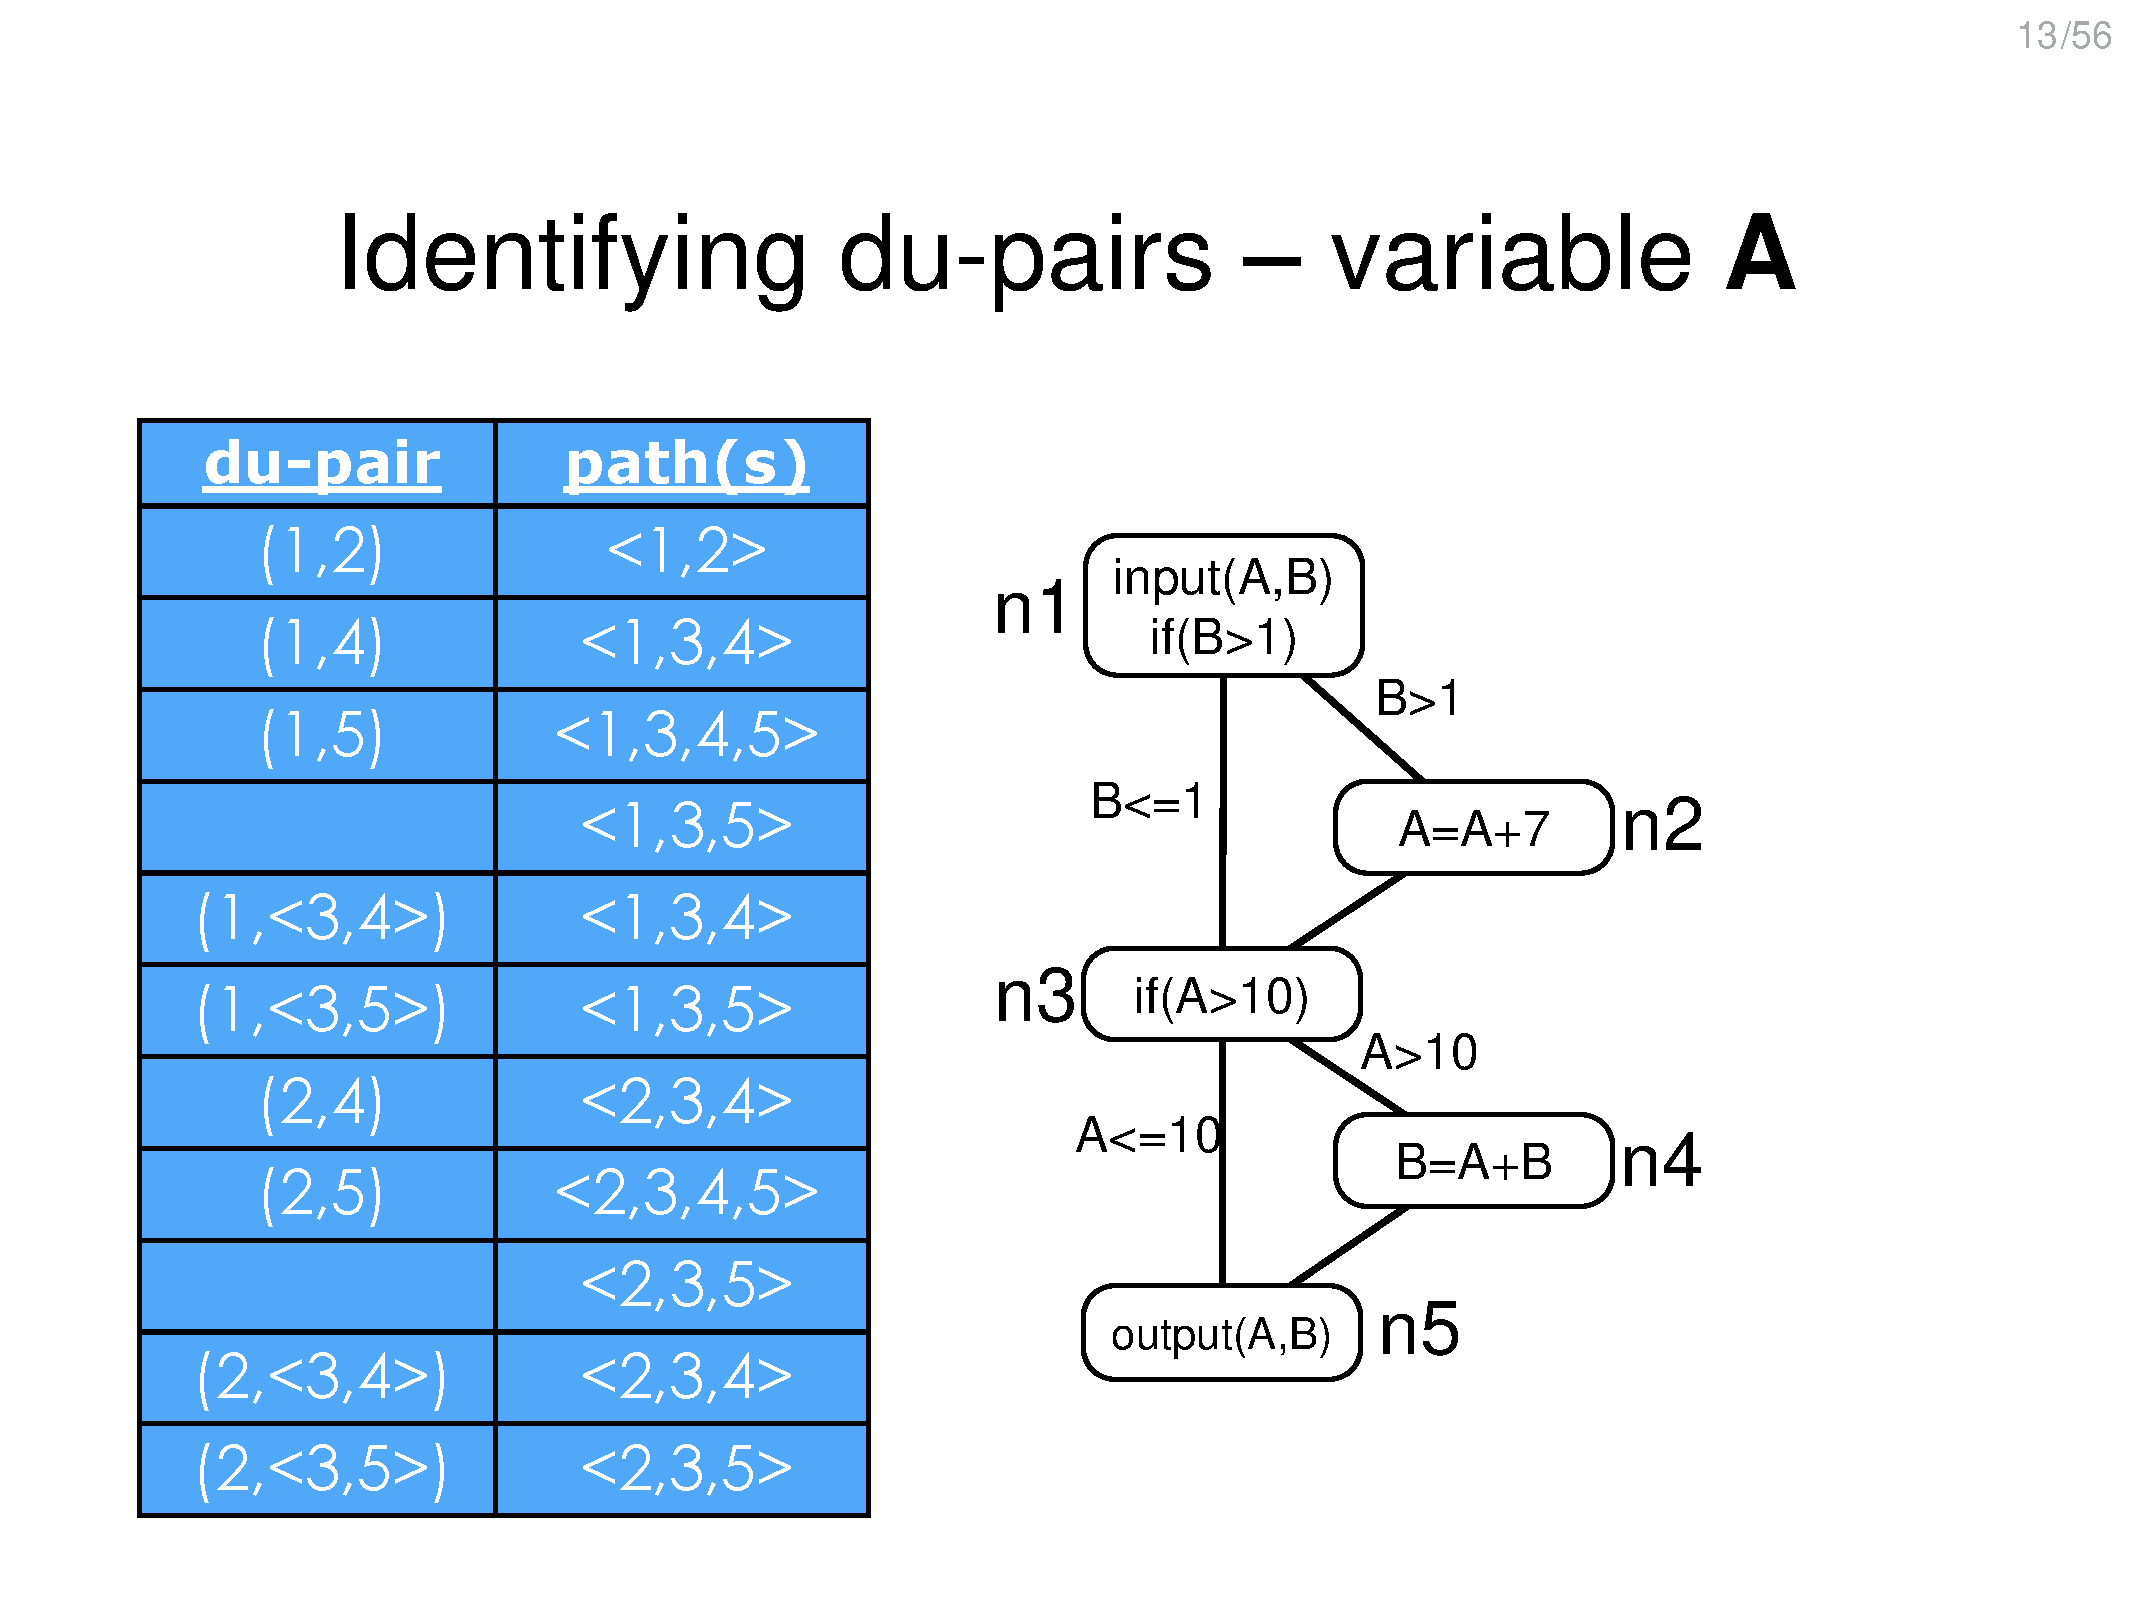
\includegraphics[width=\linewidth]{167.pdf}\\
        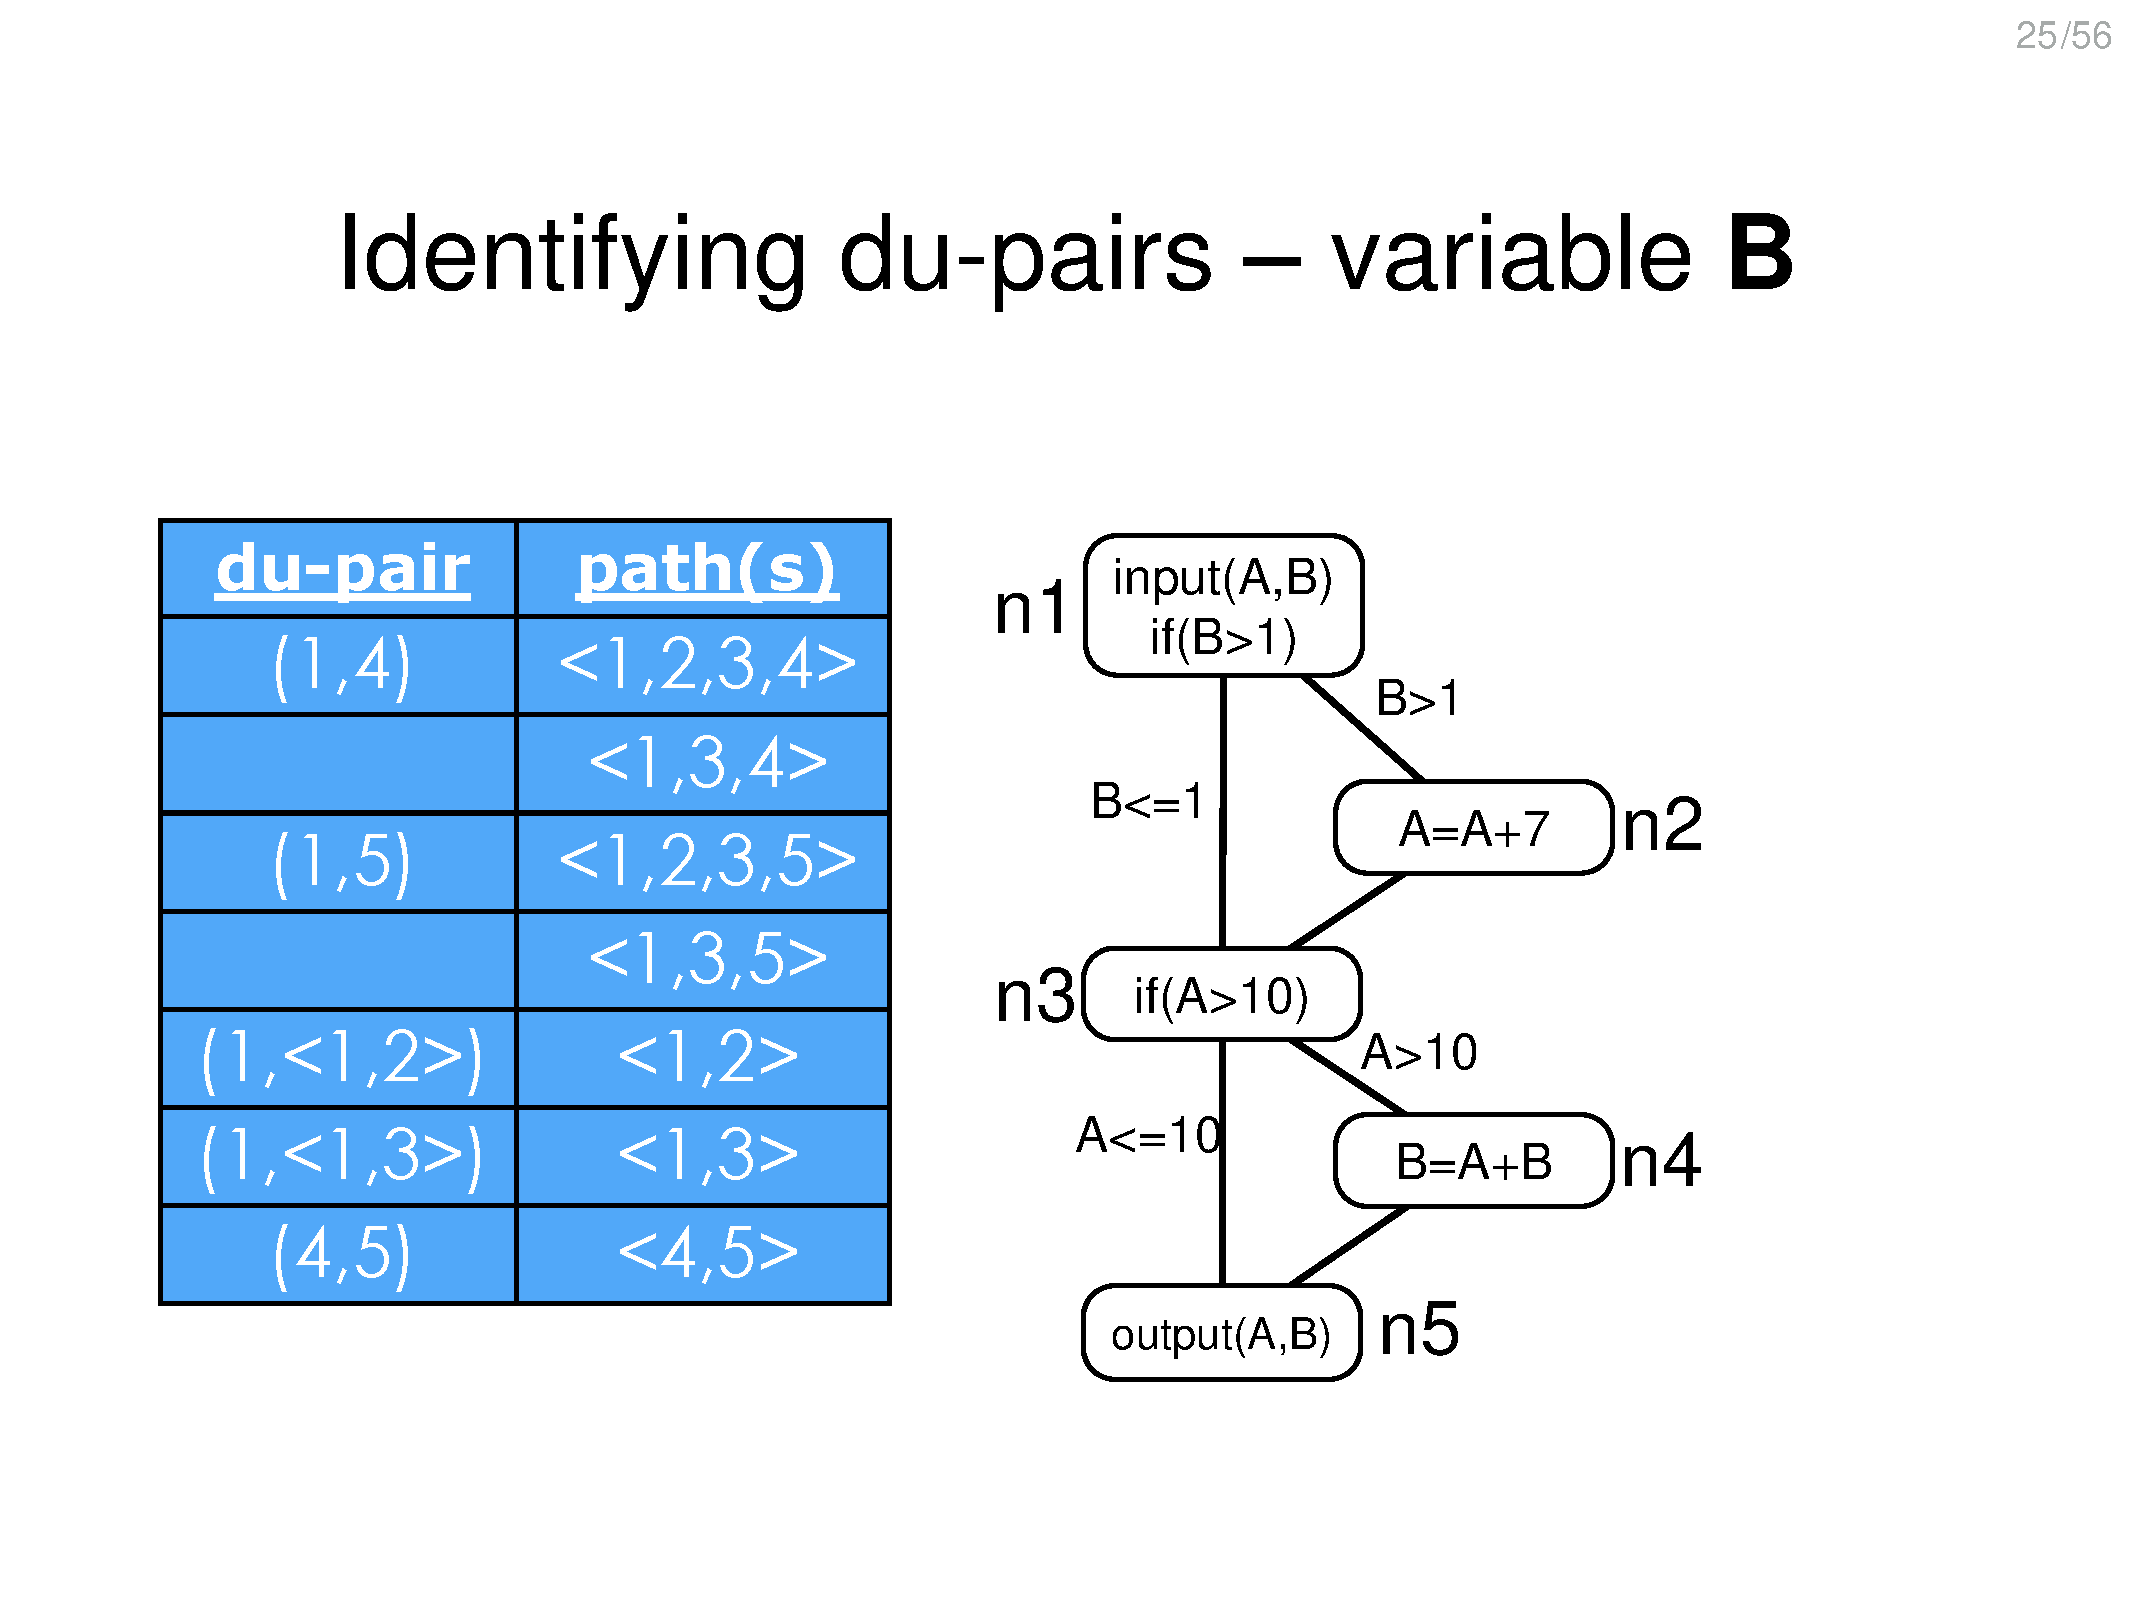
\includegraphics[width=\linewidth]{179.pdf}\\
        \textbf{\textbf{Dataflow test coverage criteria}}:\\
        \textit{All-Defs}: for every variable $v$, at least one def-clear path from every definition of $v$ to at least one c-use or p-use of $v$ must be covered\\
        \textit{All-P/C-Uses}: for every variable $v$, at least one def-clear path from every definition of $v$ to every p/c-use of $v$ must be covered\\
        \textit{All-Uses}: all du-pairs covered\\
        \textbf{Notations}:\\
        $d_1(x)$: definition of variable $x$ in node $i$\\
        $u_i(x)$: use of variable $x$ in node $i$
        $dcu(d_i(x)) = dcu(x,i)$: set of c-uses with respect to $d_1(x)$\\
        $dpu(d_i(x)) = dpu(x,i)$: set of p-uses with respect to $d_1(x)$\\
        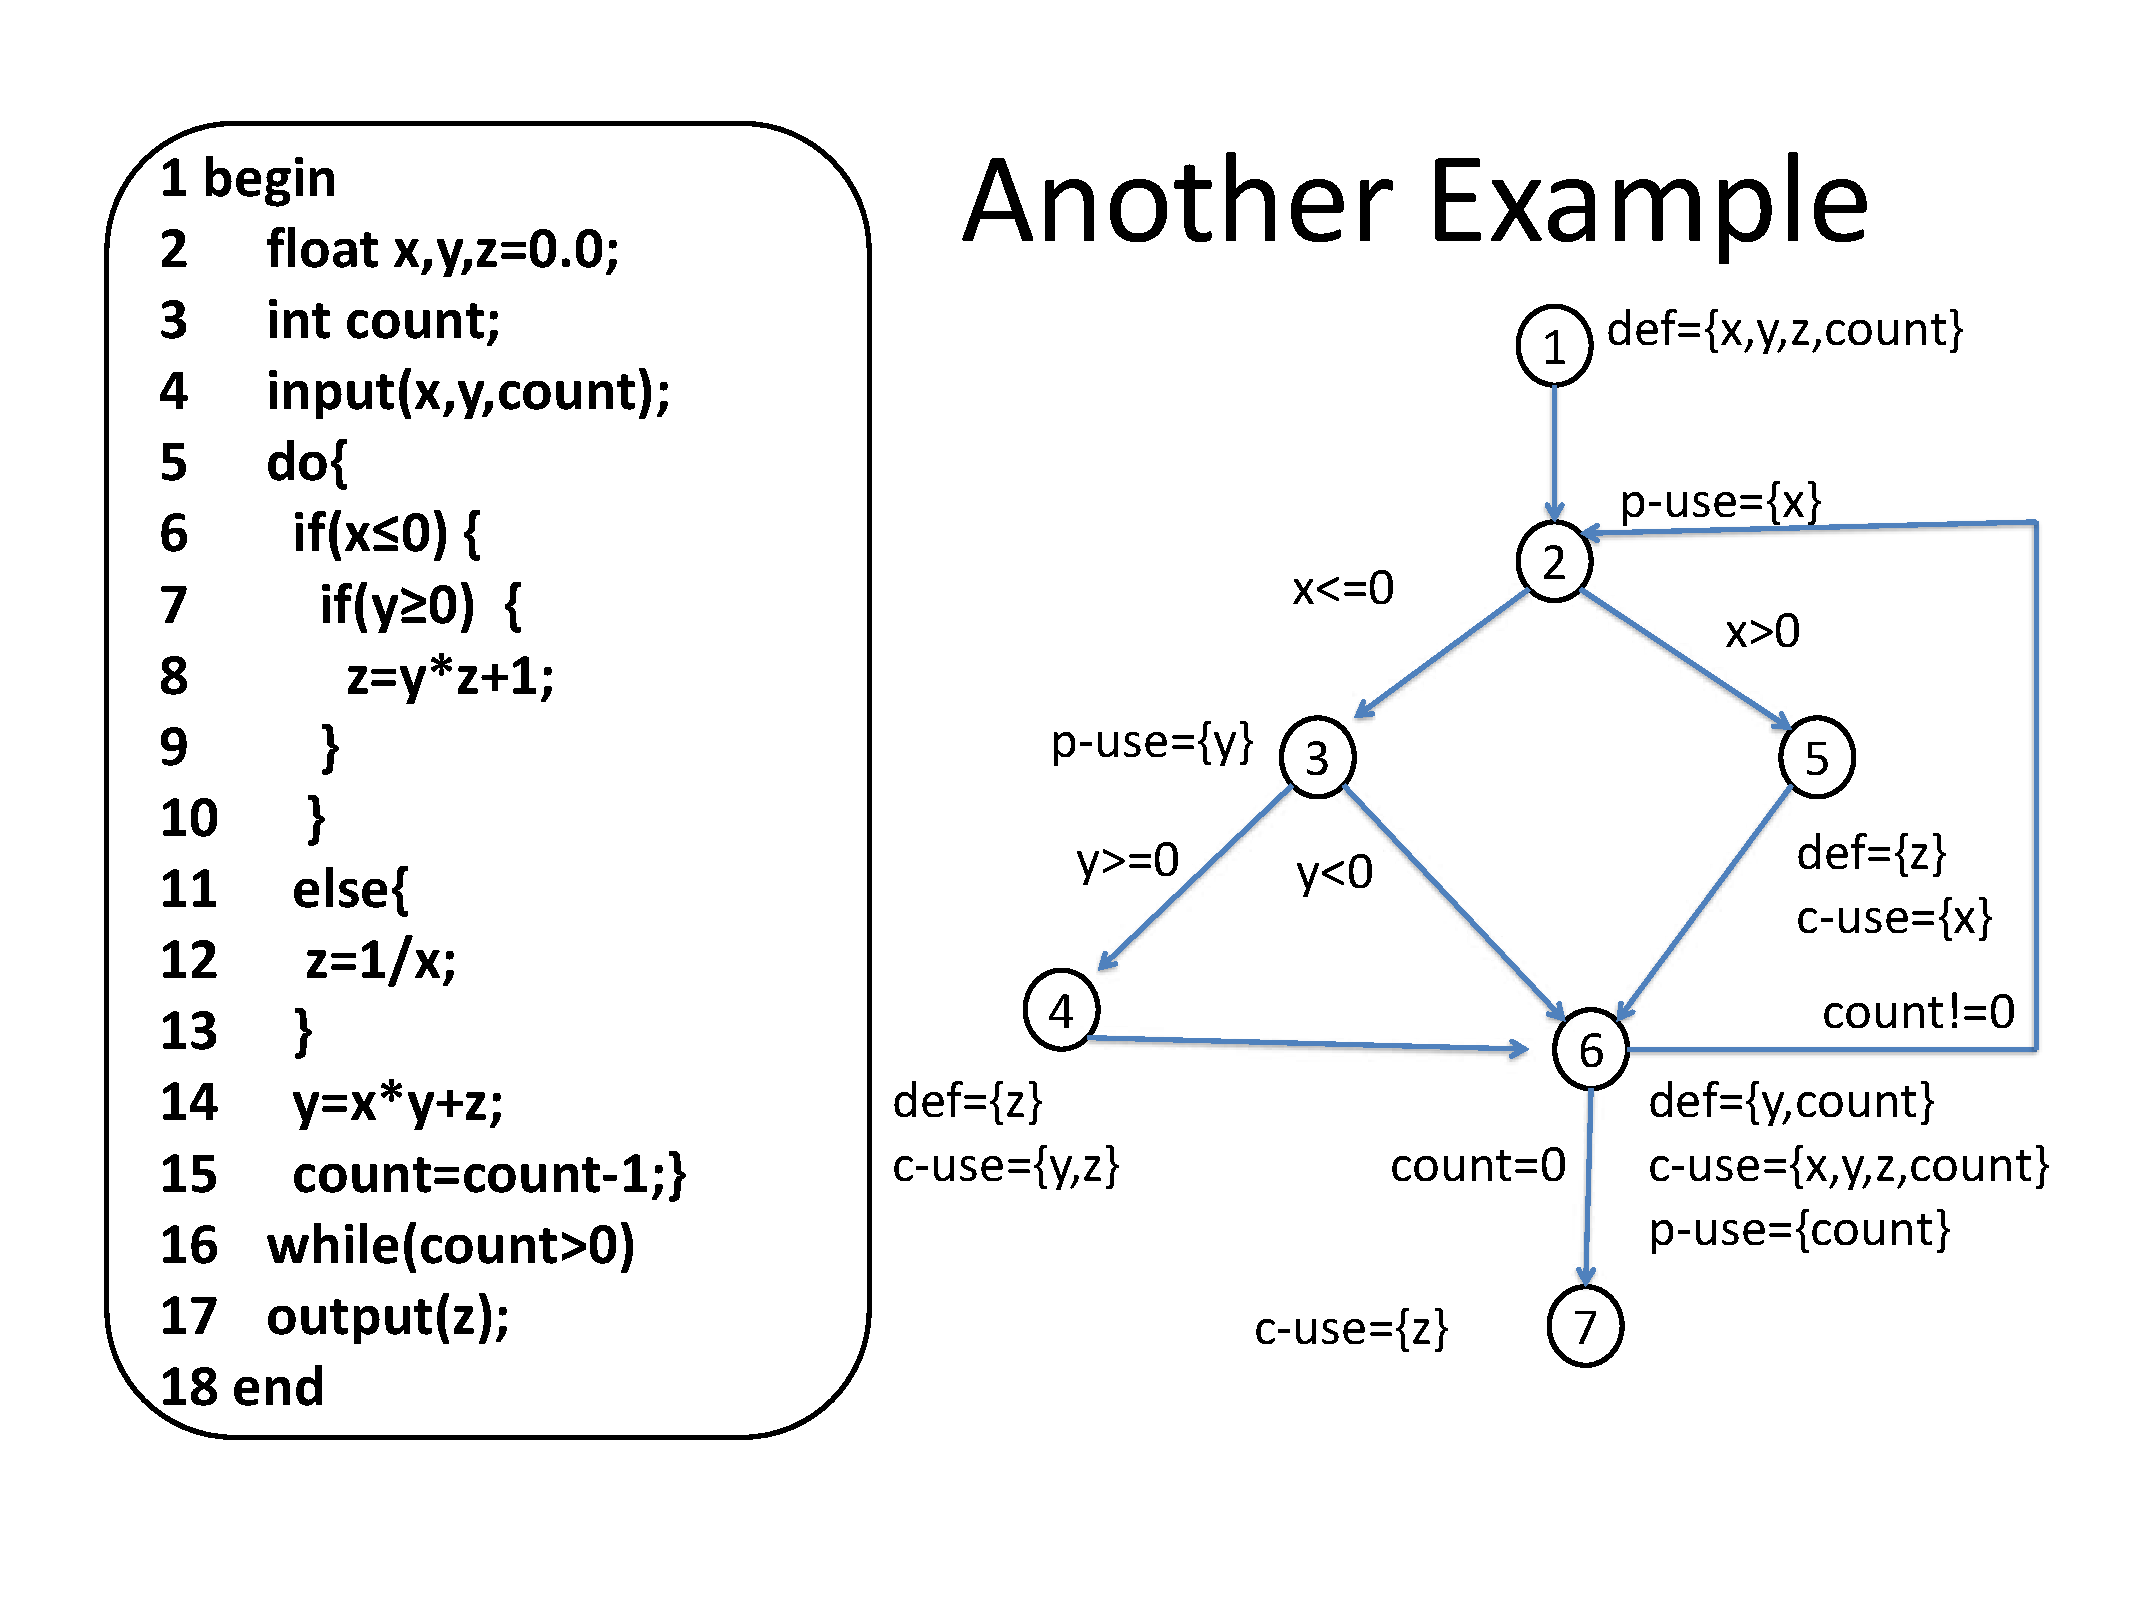
\includegraphics[width=\linewidth]{196.pdf}\\
        \textbf{All-C-Uses for above}: $dcu(x,1) + dcu(y,1) + dcu(y,6) + dcu(z,1) + dcu(z,4) + dcu(z,5) + dcu(count,1) + dcu(count,6) = 2 + 2 + 2 + 3 + 3 + 3 + 1 + 1 = 17$\\
        \textbf{All-P-Uses for above}: $dpu(x,1) + dpu(y,1) + dpu(y,6) + dpu(z,1) + dpu(z,4) + dpu(z,5) + dpu(count,1) + dpu(count,6) = 2 + 2 + 2 + 0 + 0 + 0 + 2 + 2 = 10$ (note this includes using the initial count definition even though it will always be redefined (-1) before the comparison)\\
        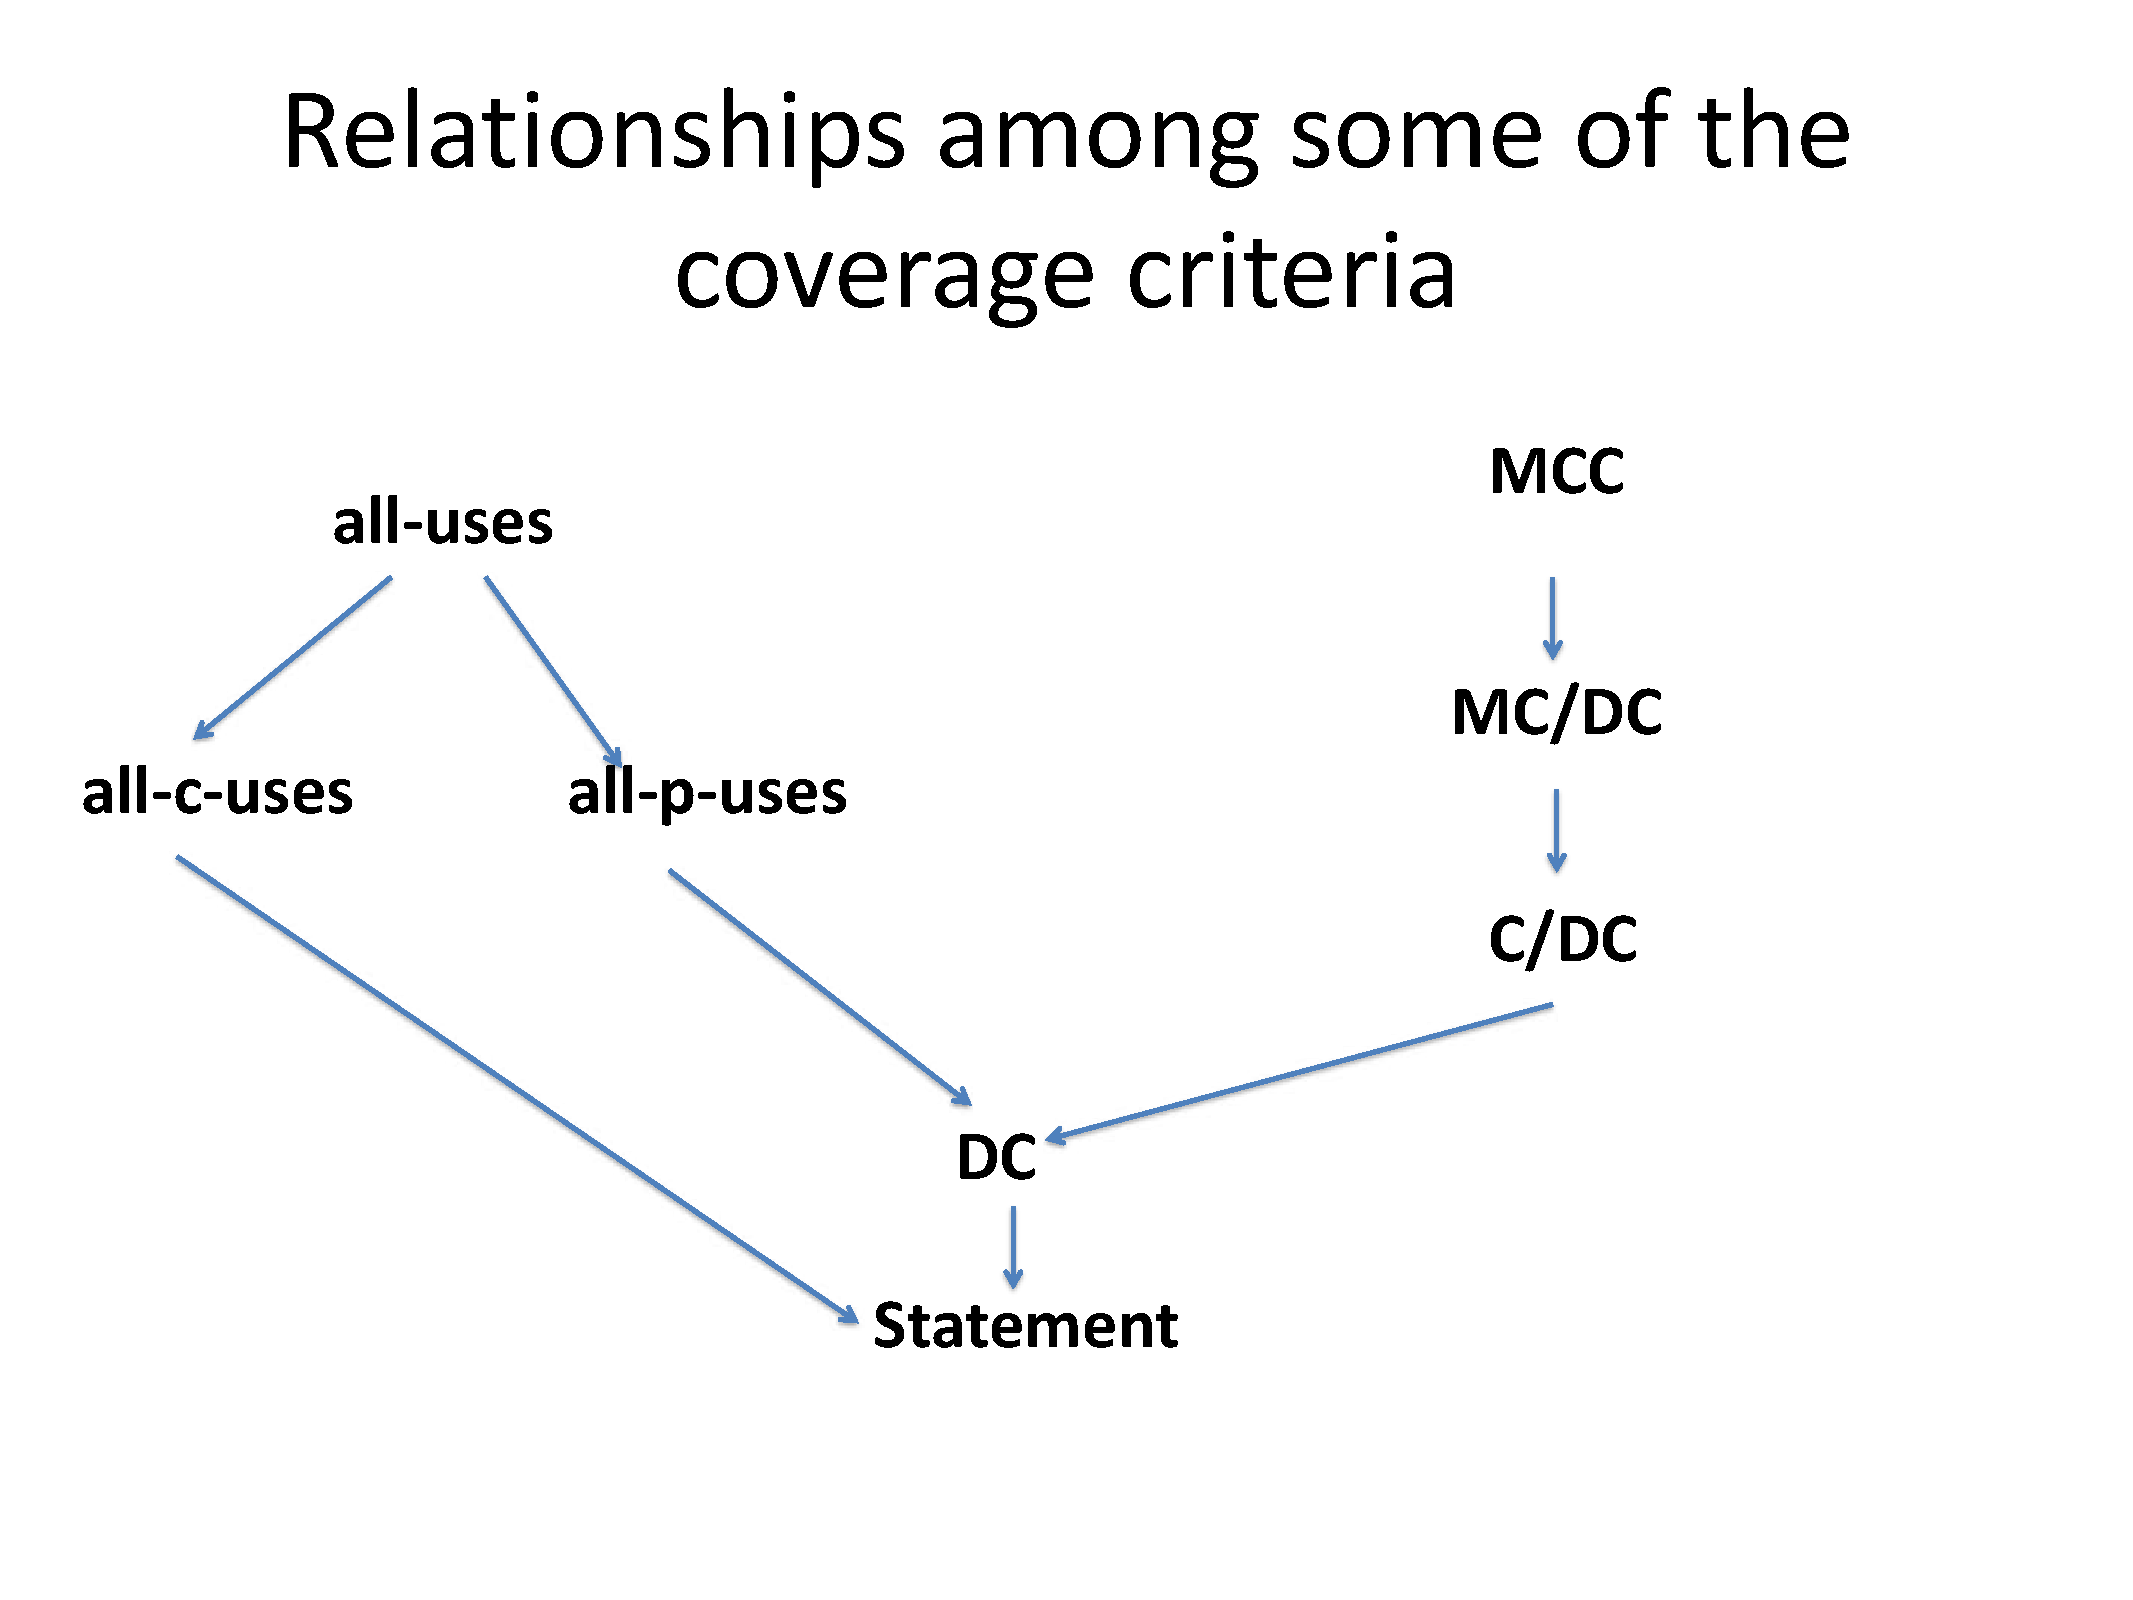
\includegraphics[width=\linewidth]{203.pdf}\\
        \vfill\null\columnbreak\noindent\underline{\textbf{Week 5}}\\
        \textbf{Program mutation}: create artificial bugs by injecting changes to statements of programs, simulate subtle bugs in real programs\\
        \textbf{Mutation testing}: software testing technique based on program mutation, can be used to evaluate test effectiveness \& enhance test suite, can be stronger than control/data-flow coverage, extremely costly since need to run whole test suite against each mutant\\
        \textbf{Mutation testing steps}: applies artificial changes based on mutation operators to generate mutants (each mutant with ony one artificial bug), run test suite against each mutant (if any test fails mutant killed, else survives), compute mutation score\\
        \textbf{Symbolic execution/evaluation}: analyse program to determine what inputs cause each part of program to execute, execute programs with symbols (track symbolic state rather than concrete input, when execute one path actually simulate many test inputs (since considering all inputs that can exercise same path))\\
        \textbf{Problems with symbolic execution}:\\
        \textit{Path explosion}: $2^n$ paths for $n$ branches, infinite paths for unbounded loops, calculate constraints for all paths is infeasible for real software\\
        \textit{Constraint too complex}: especially for large programs, also it is NP-complete\\
        \textbf{Input sub-domain}: set of inputs satisfying path condition\\
        \textbf{Searching input to execute path}: equivalent to solving associated path condition\\
        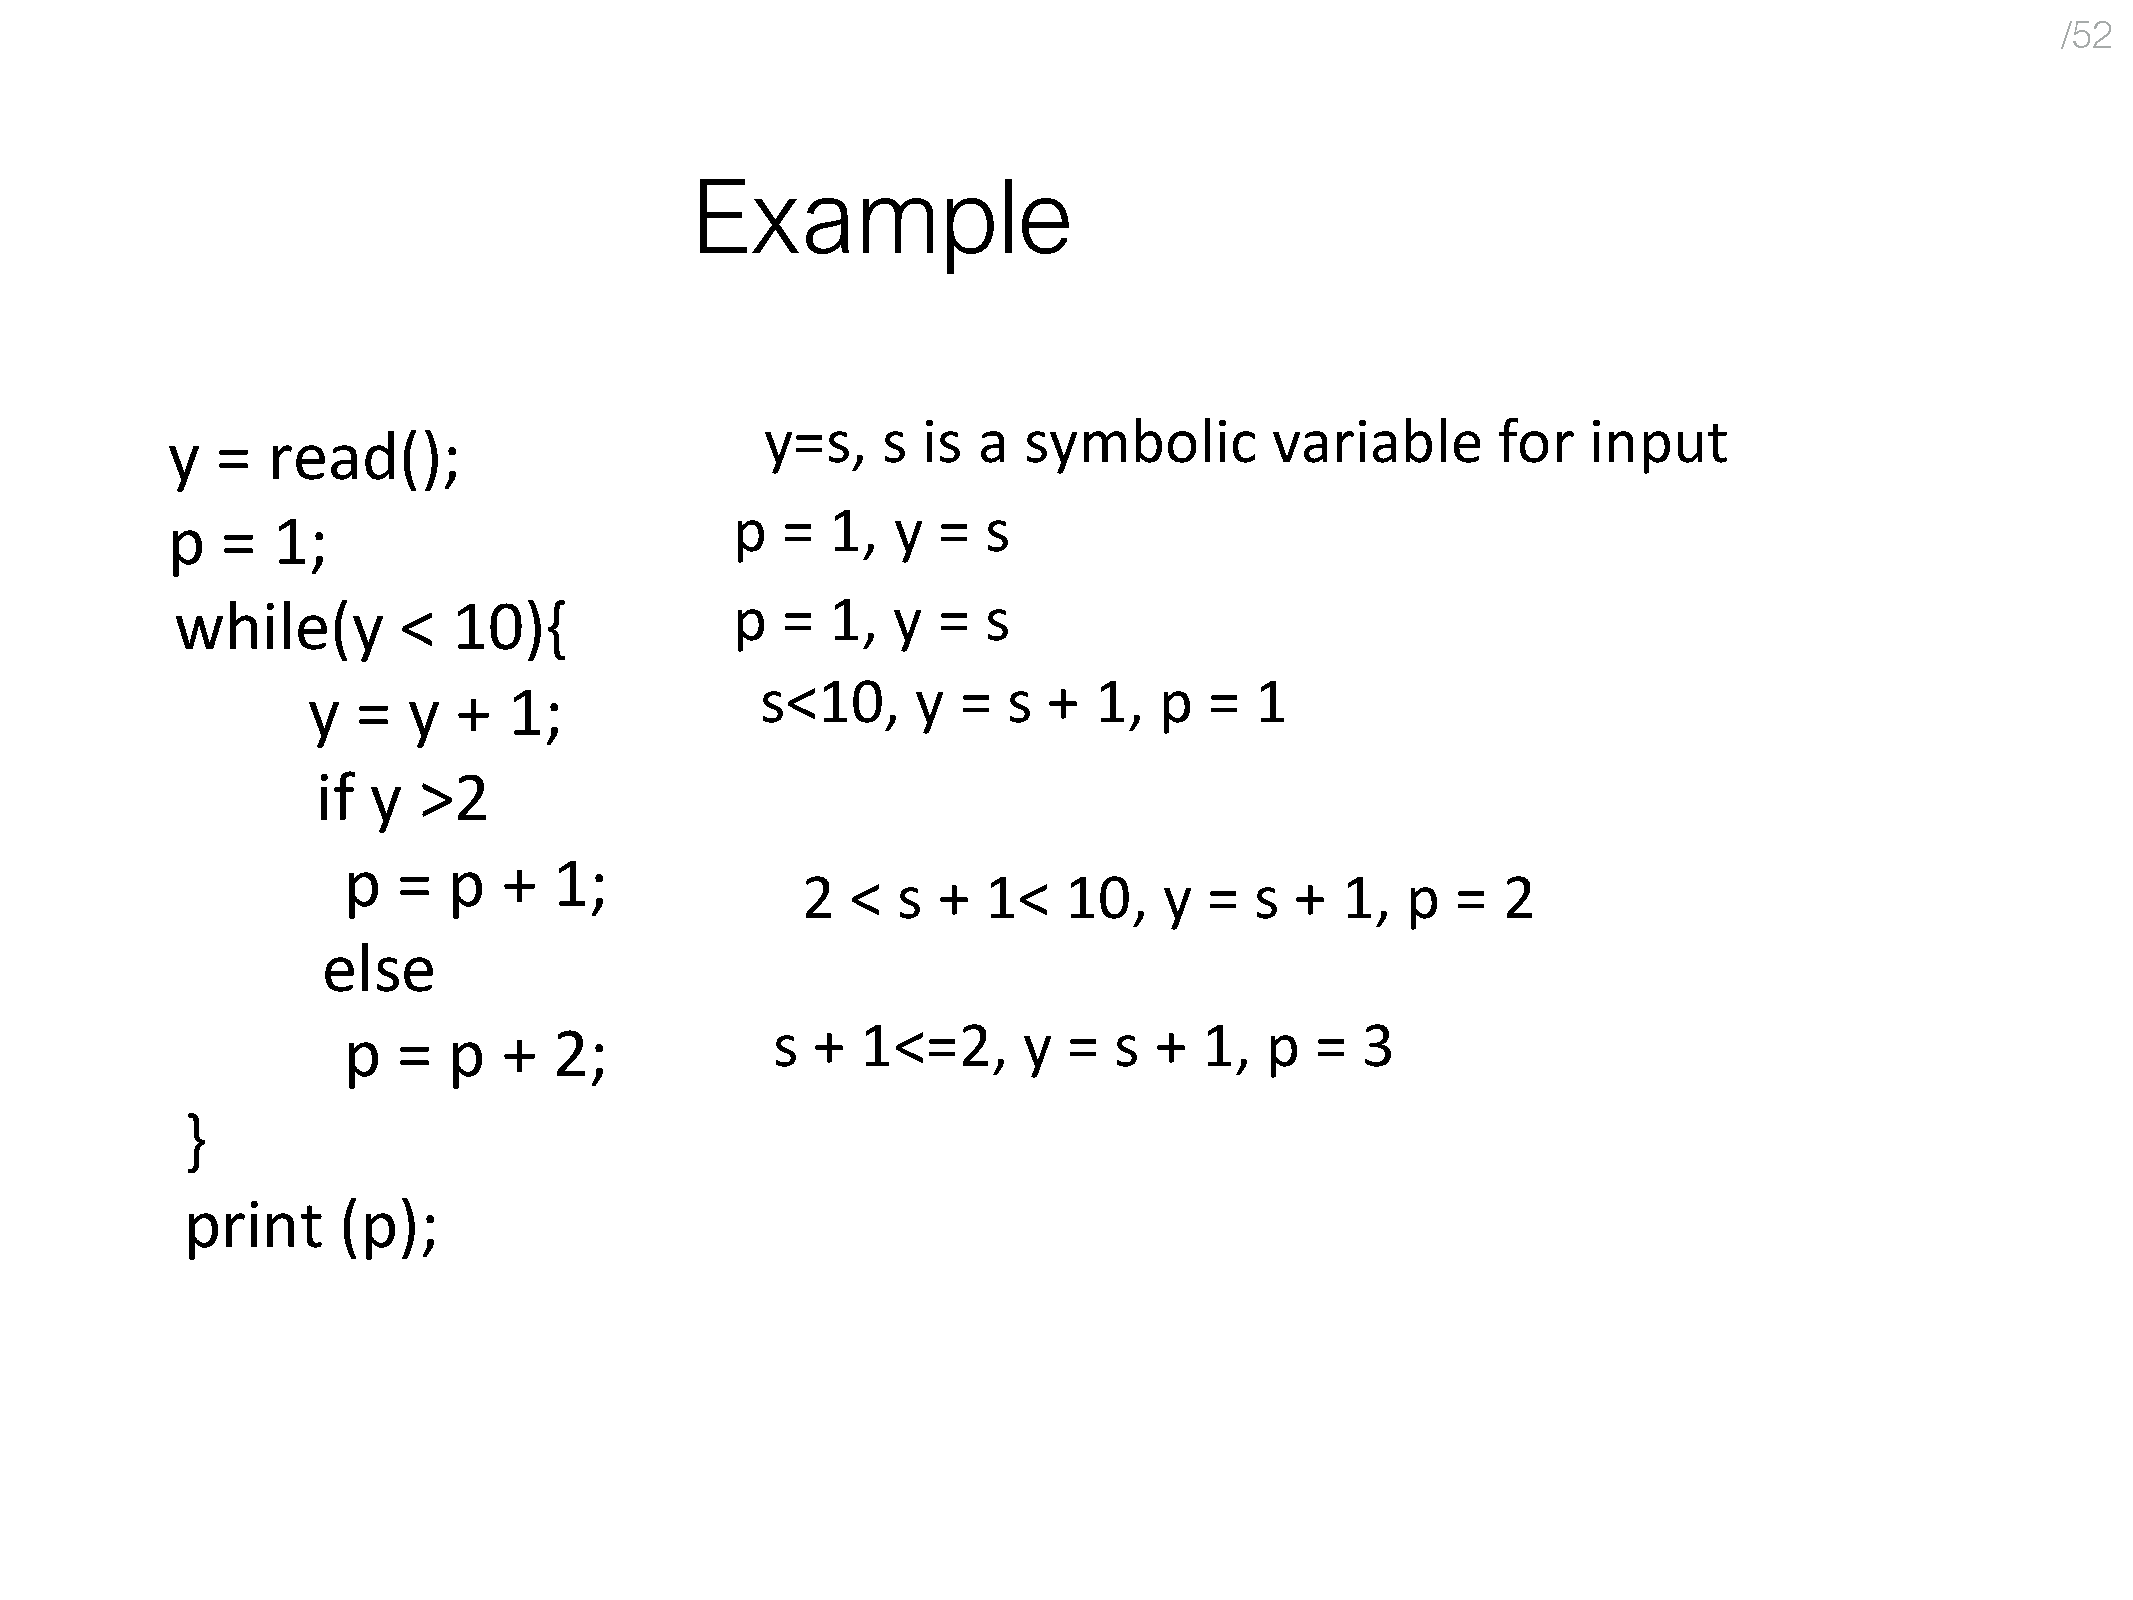
\includegraphics[width=\linewidth]{242.pdf}\\
        \vfill\null\columnbreak\noindent\underline{\textbf{Week 6}}\\
        \textbf{Random testing}: random number generator (monkeys) to generate test cases, also called fuzz testing, monkey testing, slelect tests from entire input domain (set of all possible inputs) randomly \& independently, no guide towards failure-causing inputs\\
        \textbf{Adaptive Random Testing}: achieve even spread of test cases\\
        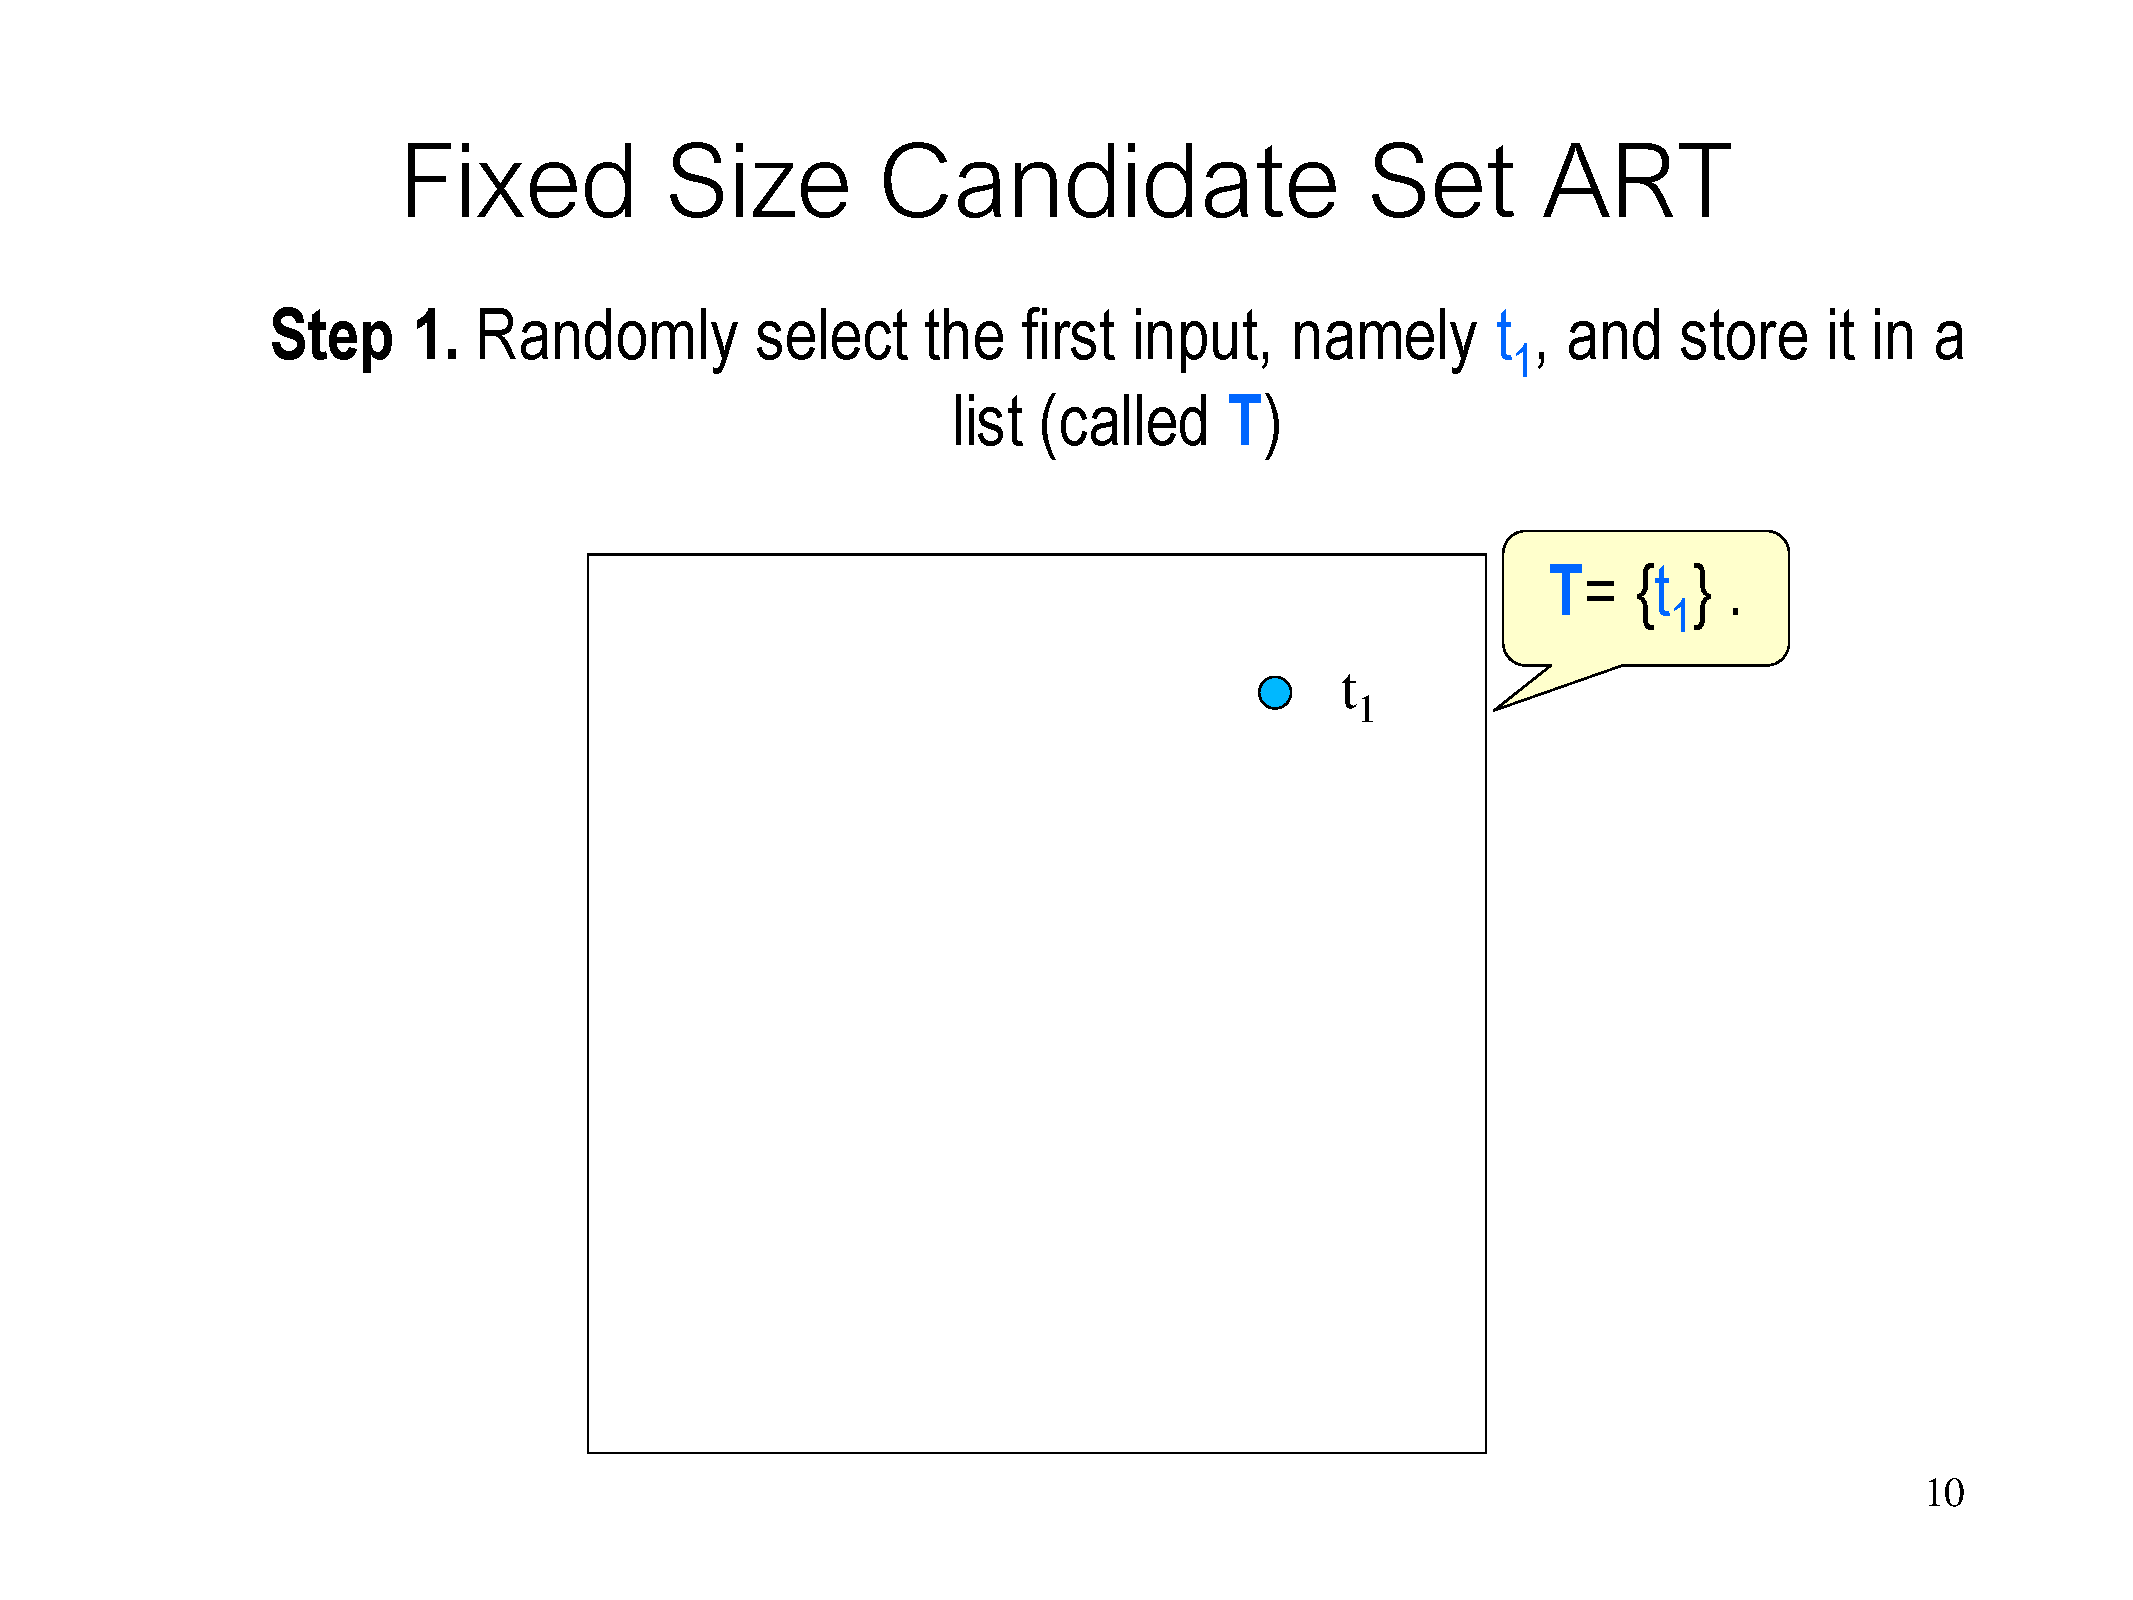
\includegraphics[width=\linewidth]{259.pdf}\\
        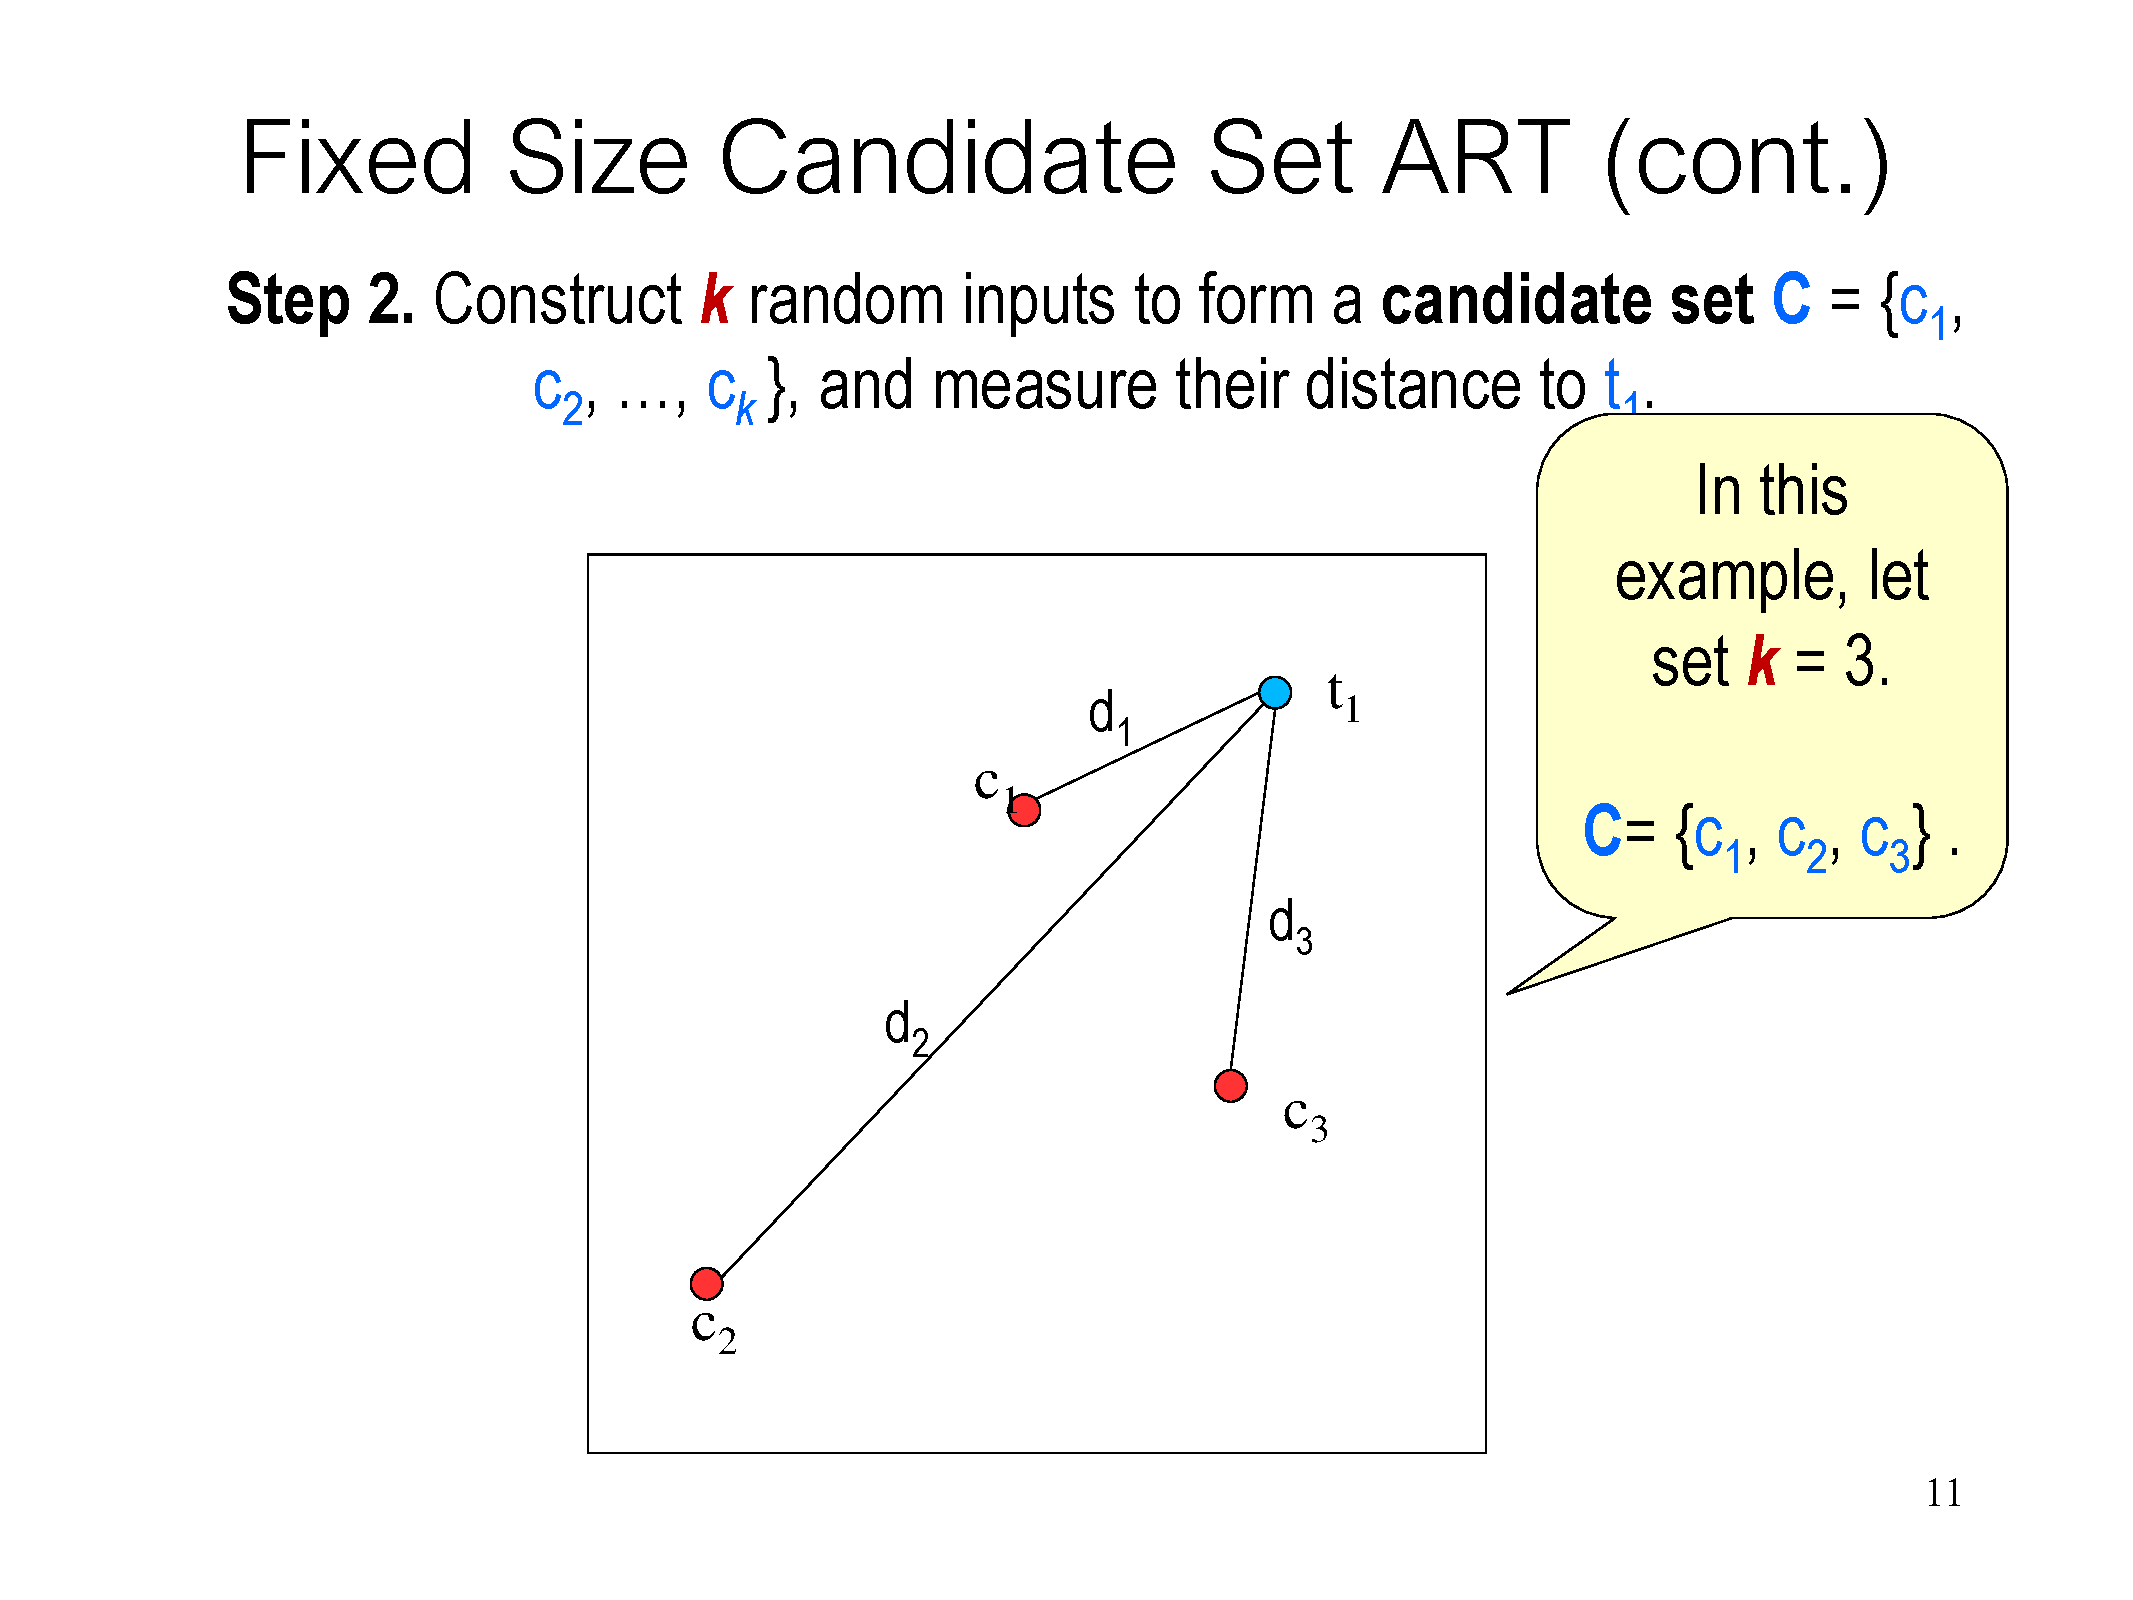
\includegraphics[width=\linewidth]{260.pdf}\\
        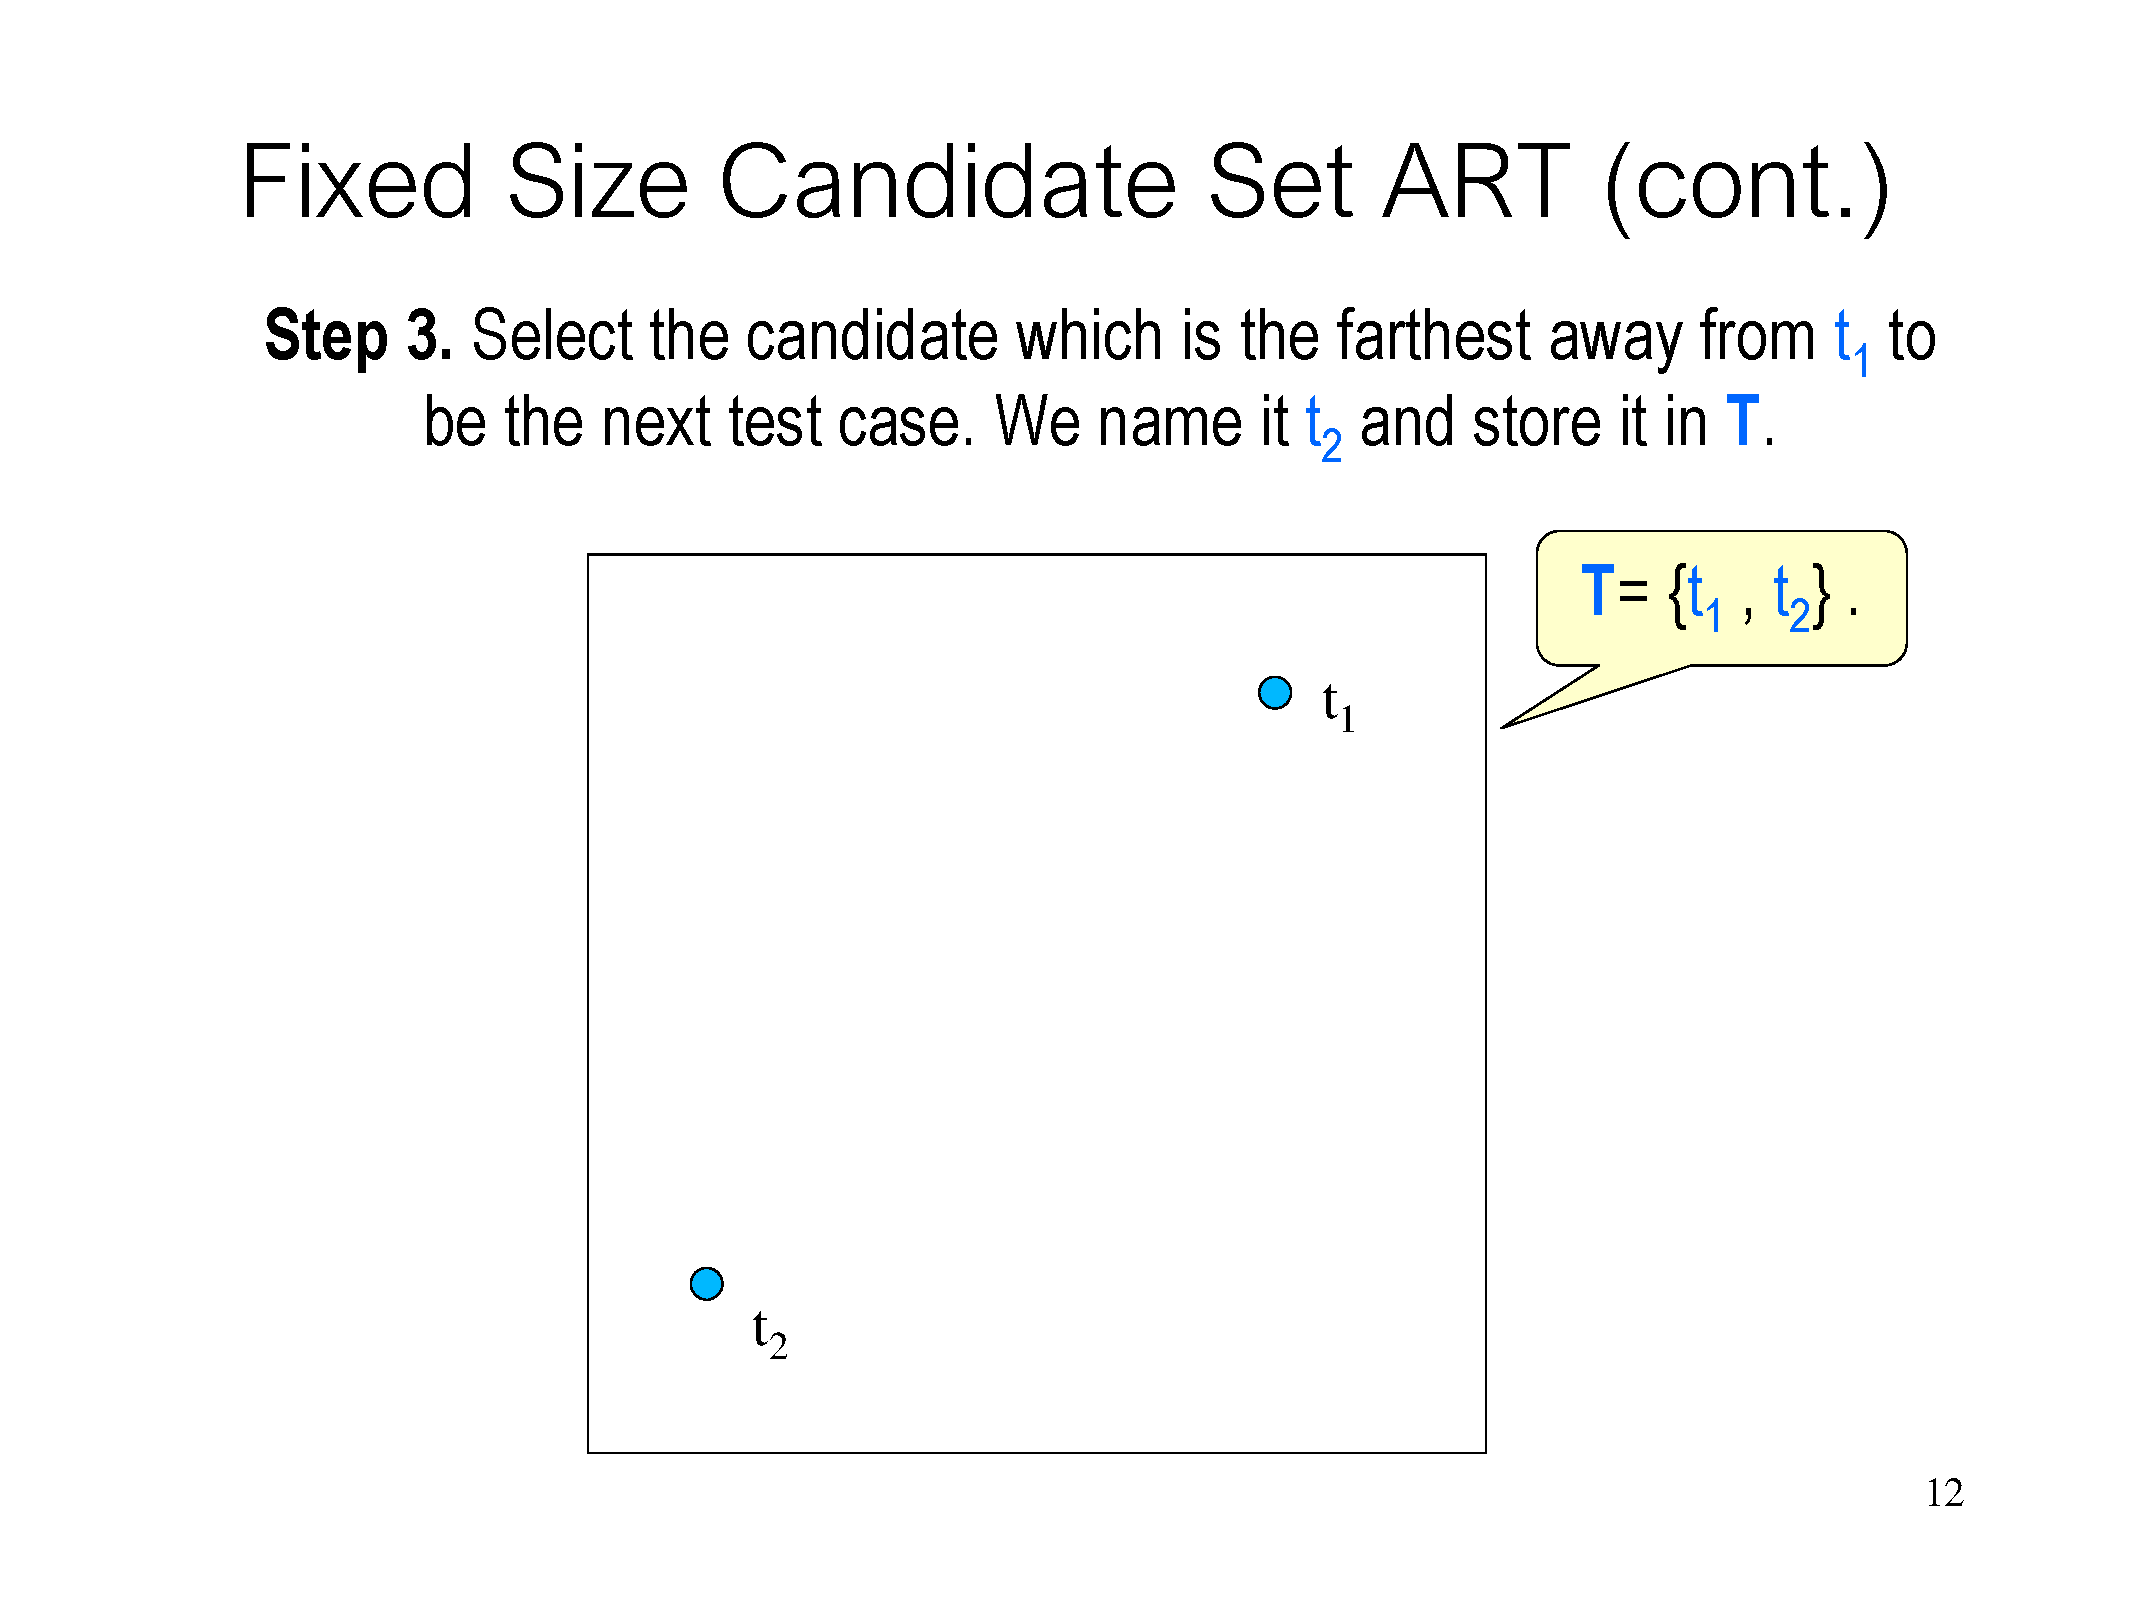
\includegraphics[width=\linewidth]{261.pdf}\\
        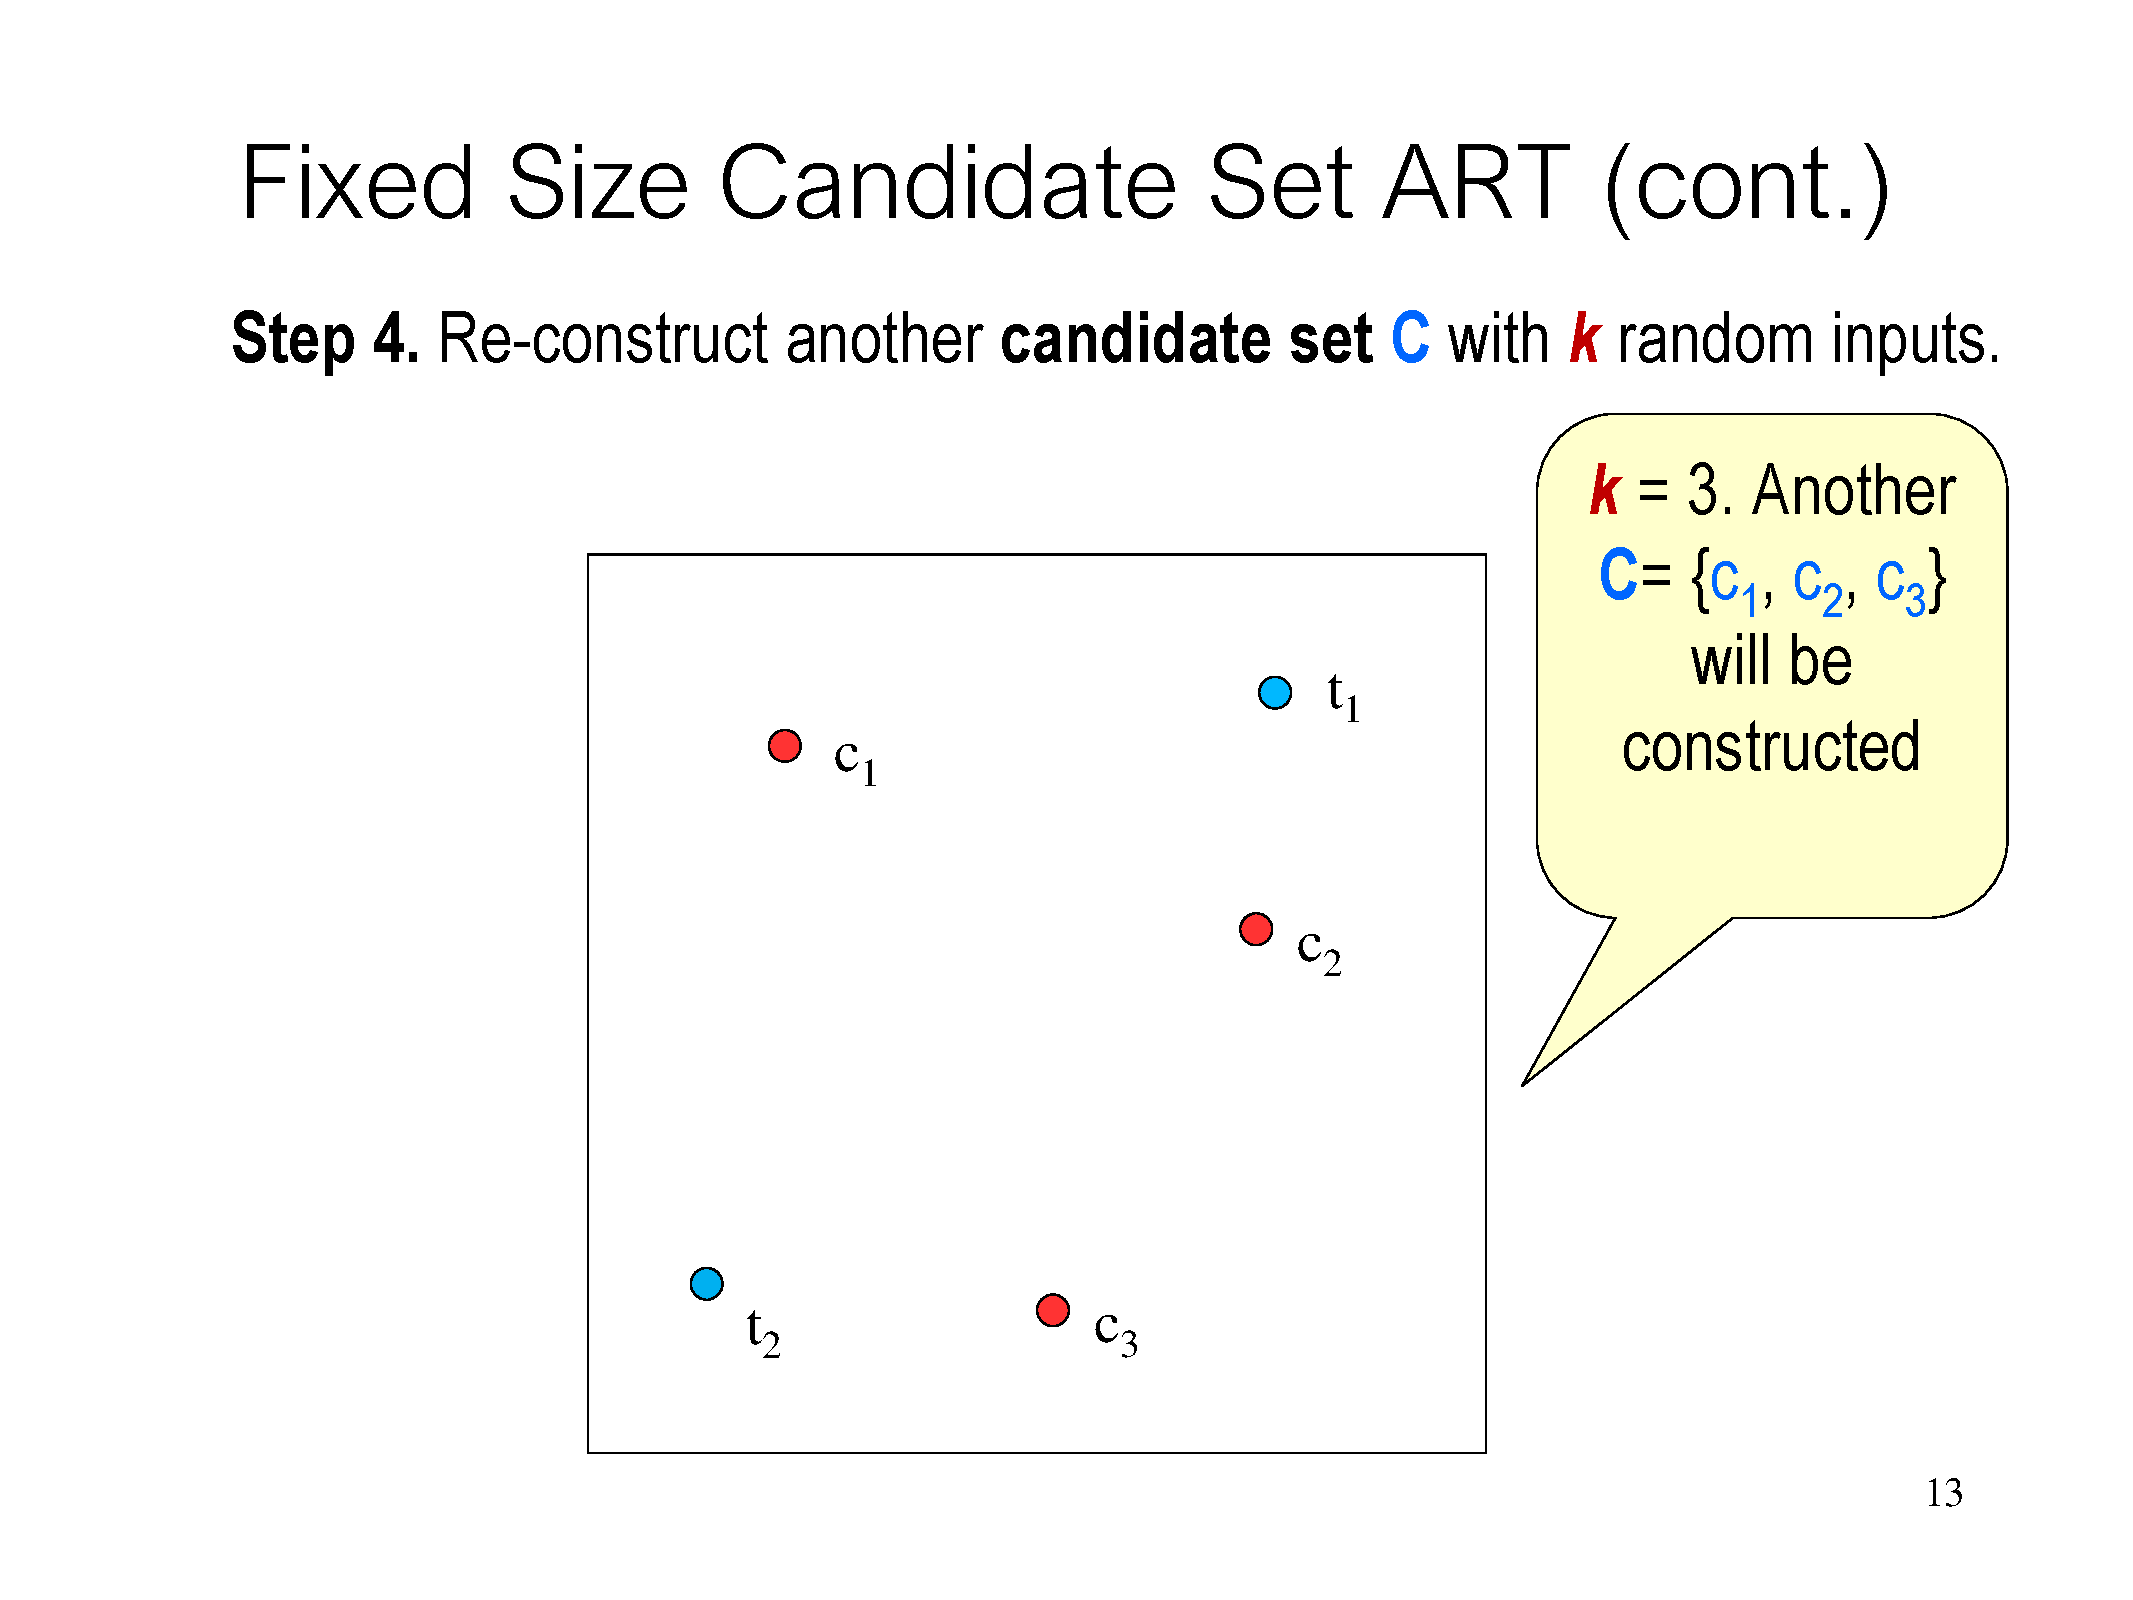
\includegraphics[width=\linewidth]{262.pdf}\\
        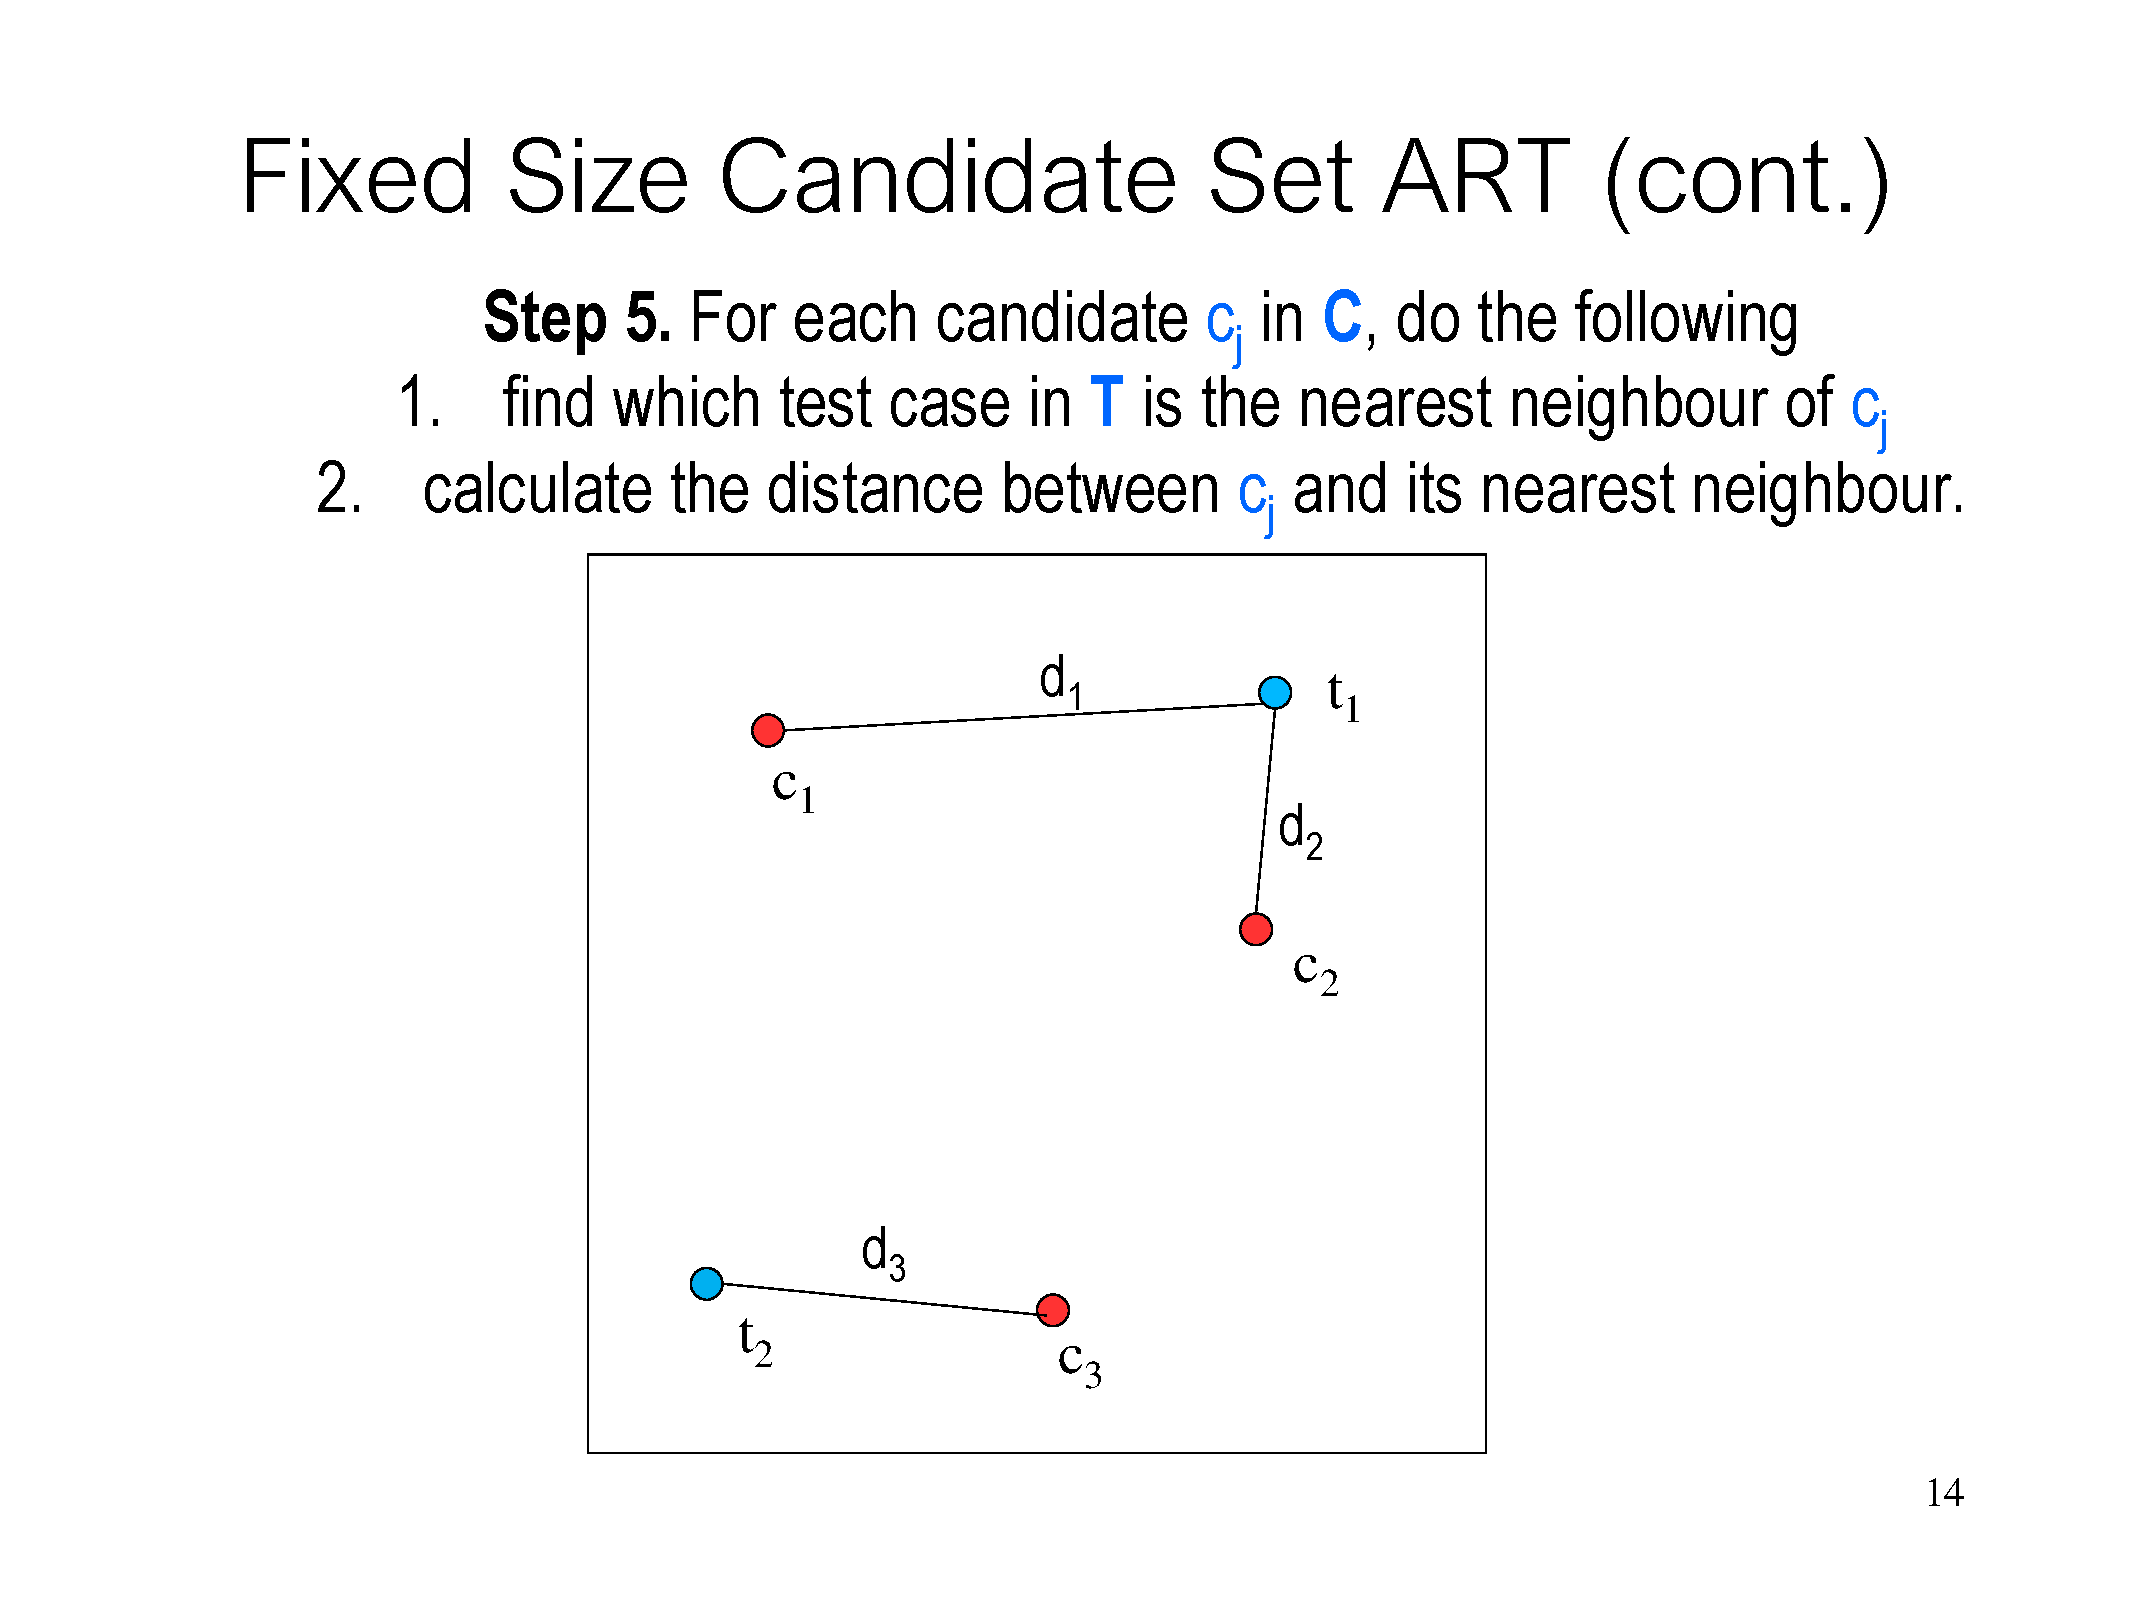
\includegraphics[width=\linewidth]{263.pdf}\\
        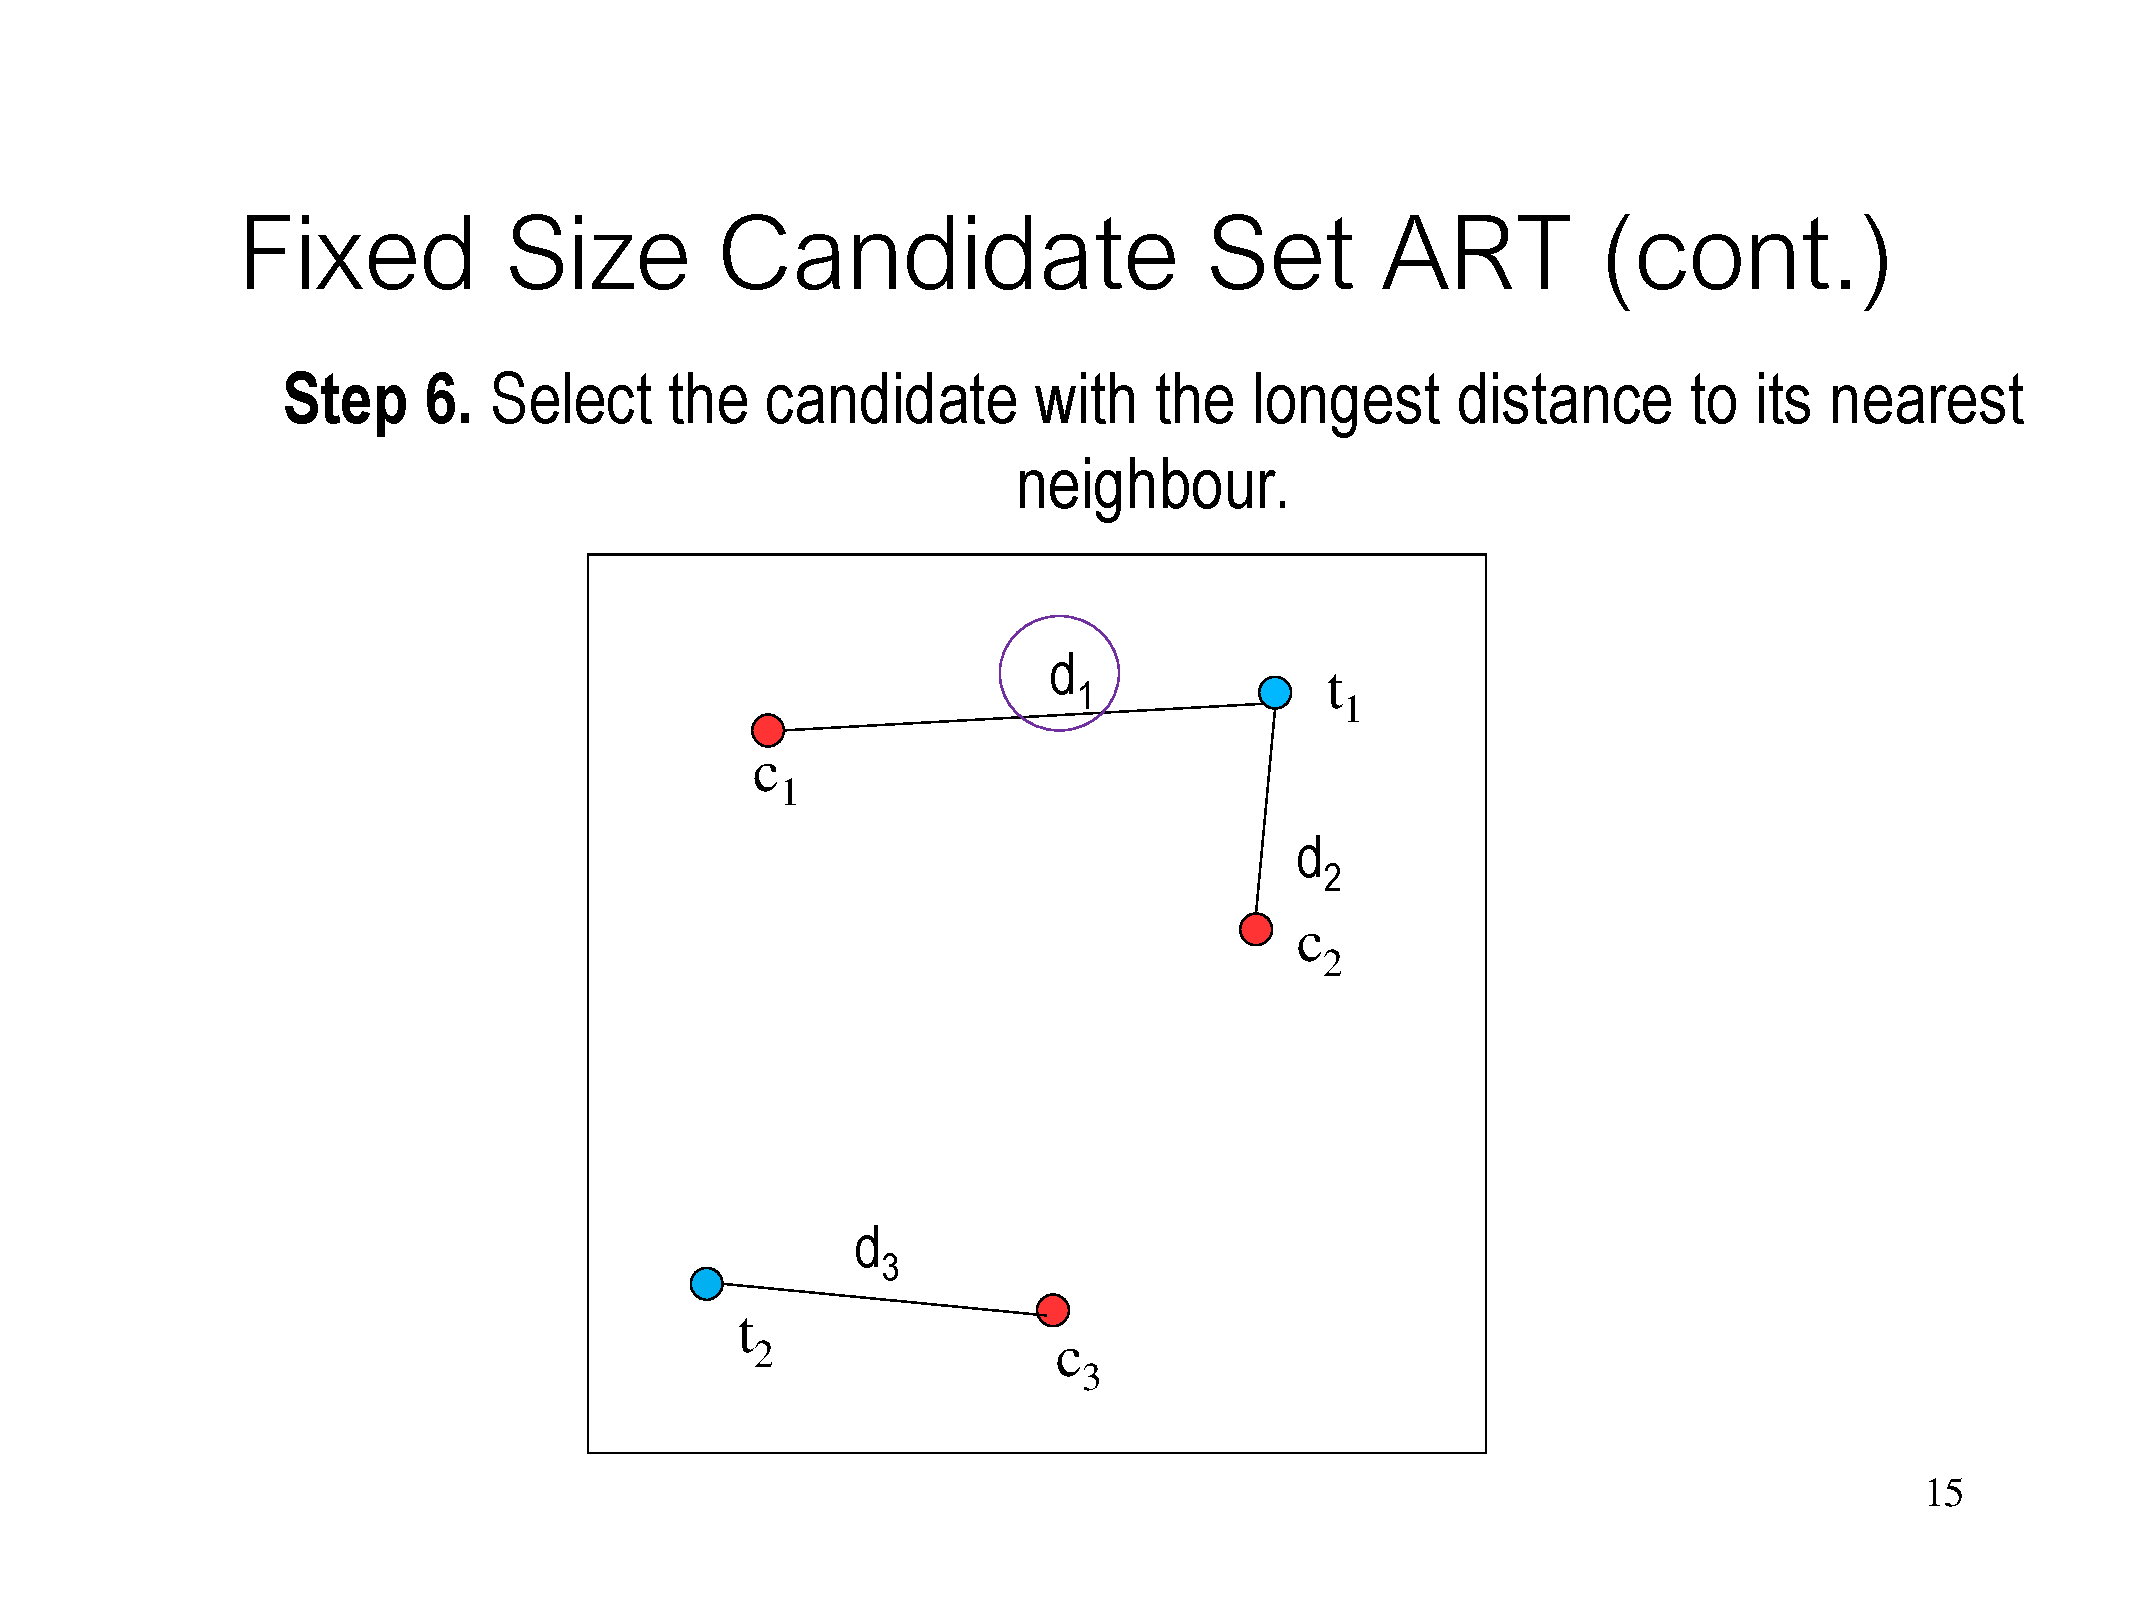
\includegraphics[width=\linewidth]{264.pdf}\\
        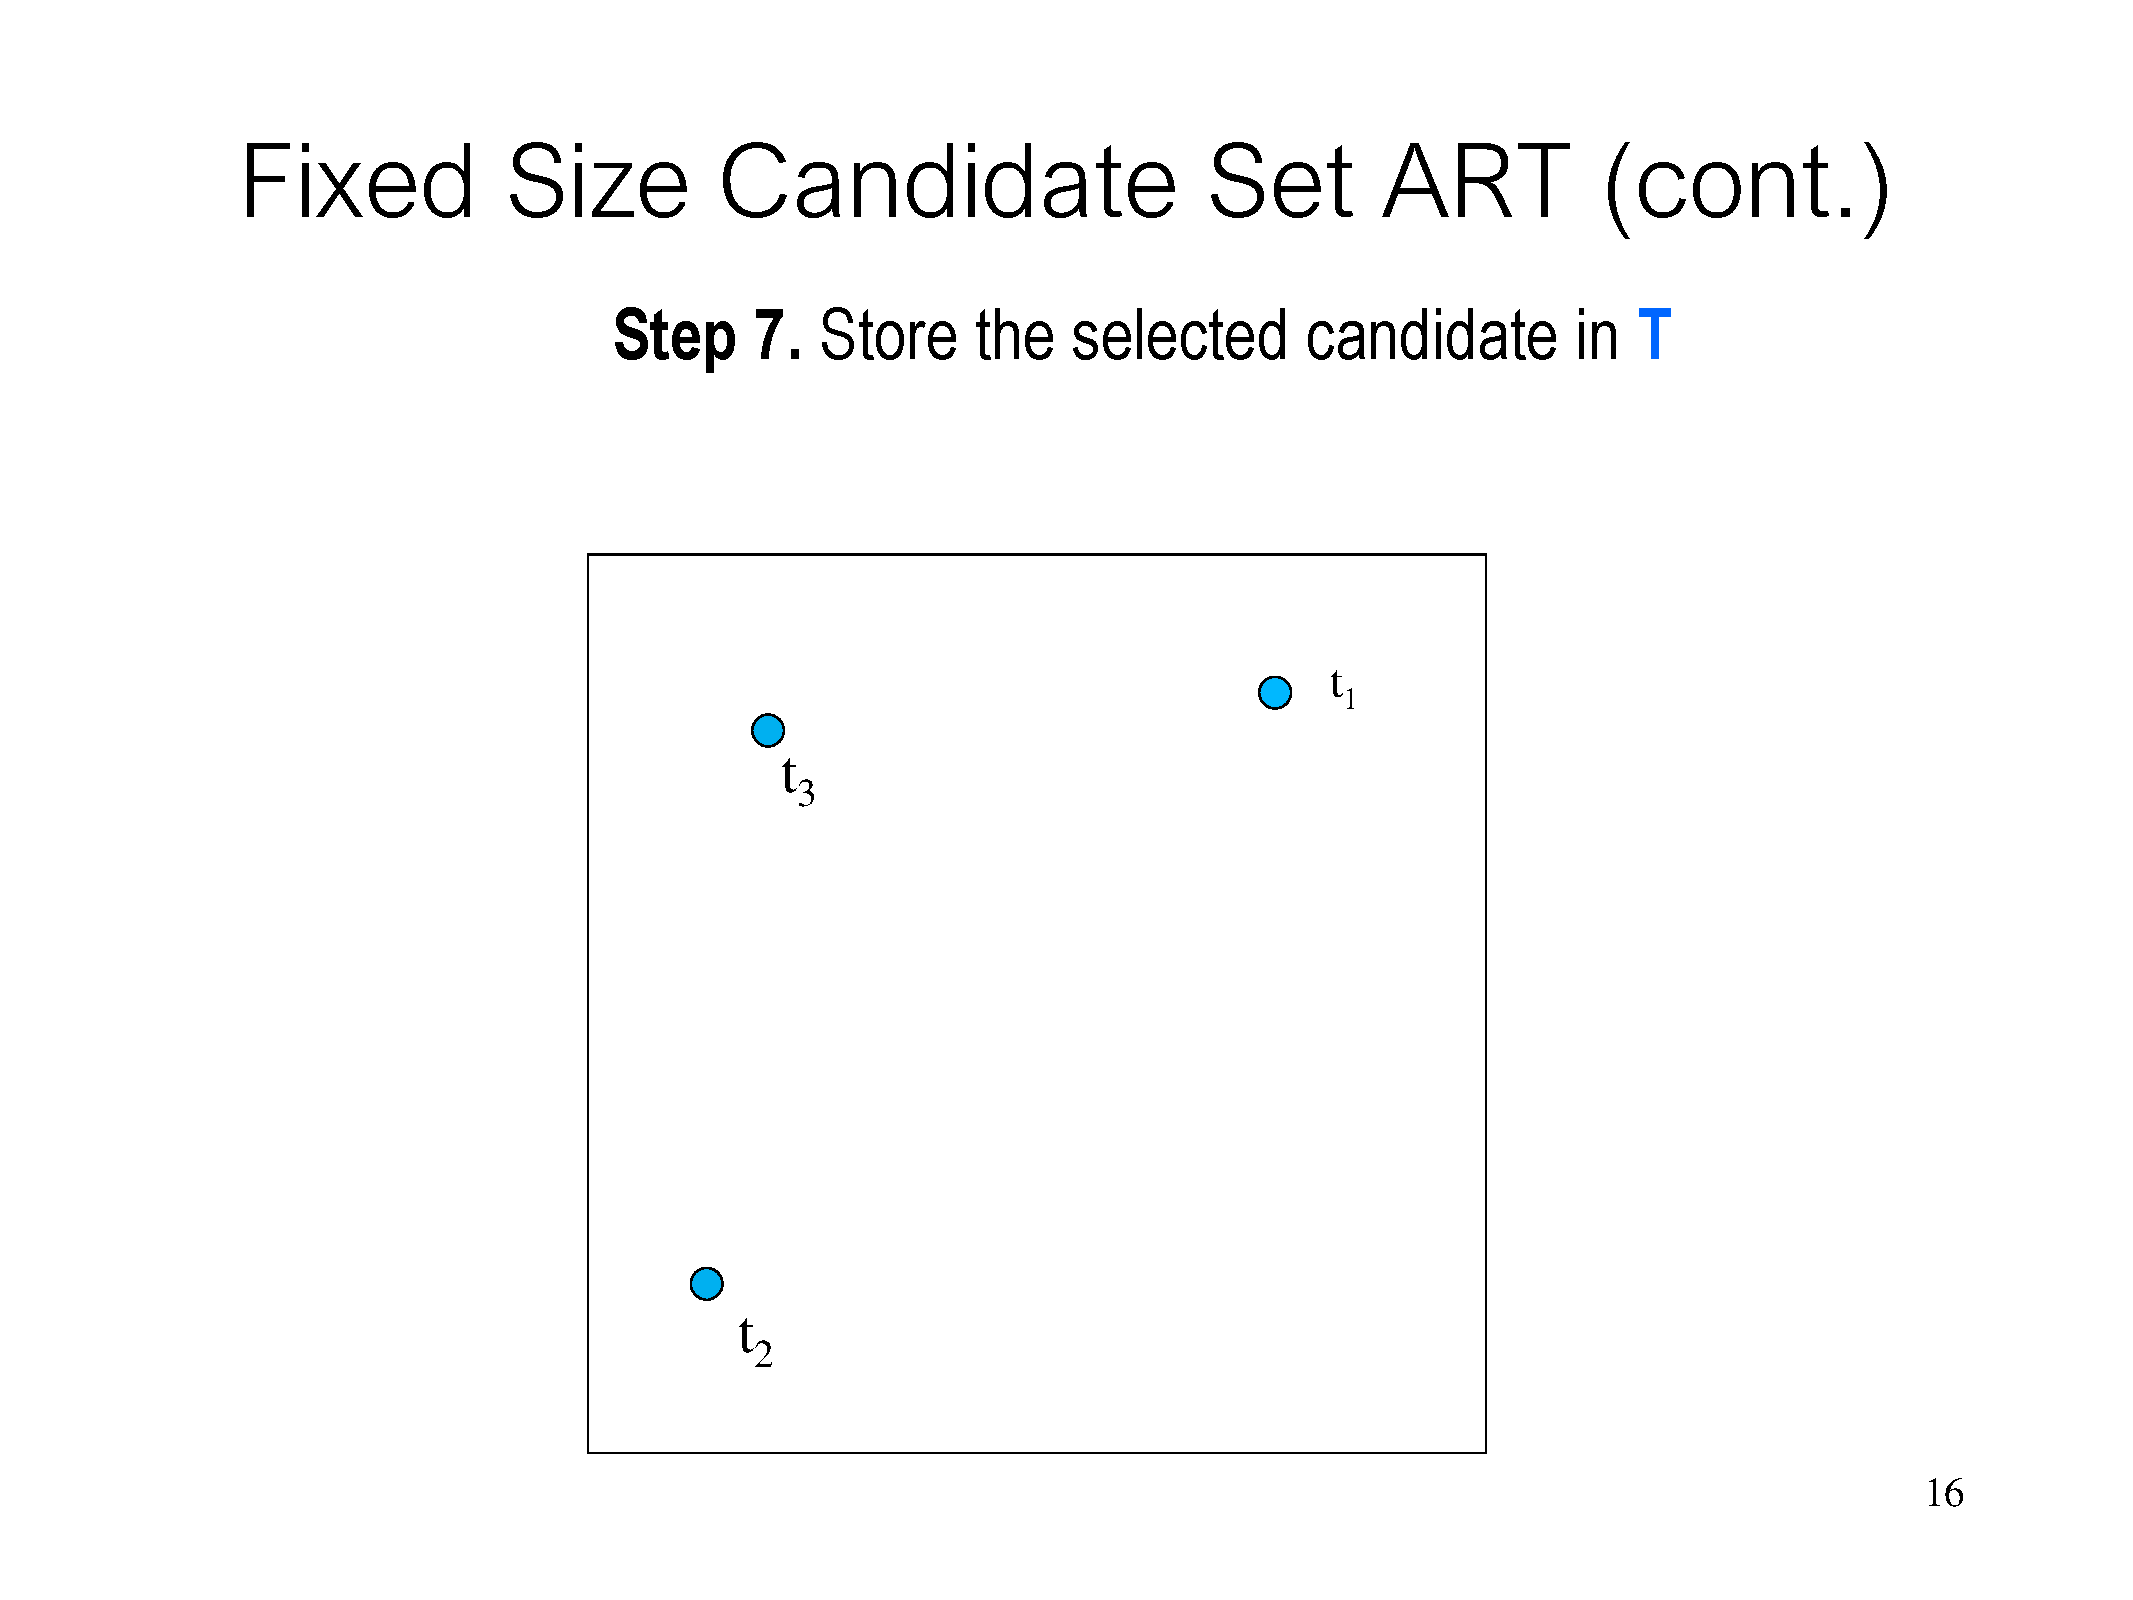
\includegraphics[width=\linewidth]{265.pdf}\\
        \textbf{Distance in ART}: can use Euclidean distance, if $p = (p_1, p_2, \ldots, P_n)$ \& $q = (q_1, q_2, \ldots, q_n)$ are 2 points in $n$-dimensional space, $d(p,q) = d(q,p) = \sqrt{{(q_1 - p_1)}^2 + {(q_2 - p_2)}^2 + \cdots + {(q_n-p_n)}^2} = \sqrt{\sum\nolimits_{i=1}^{n}{(q_i-p_i)}^2}$\\
        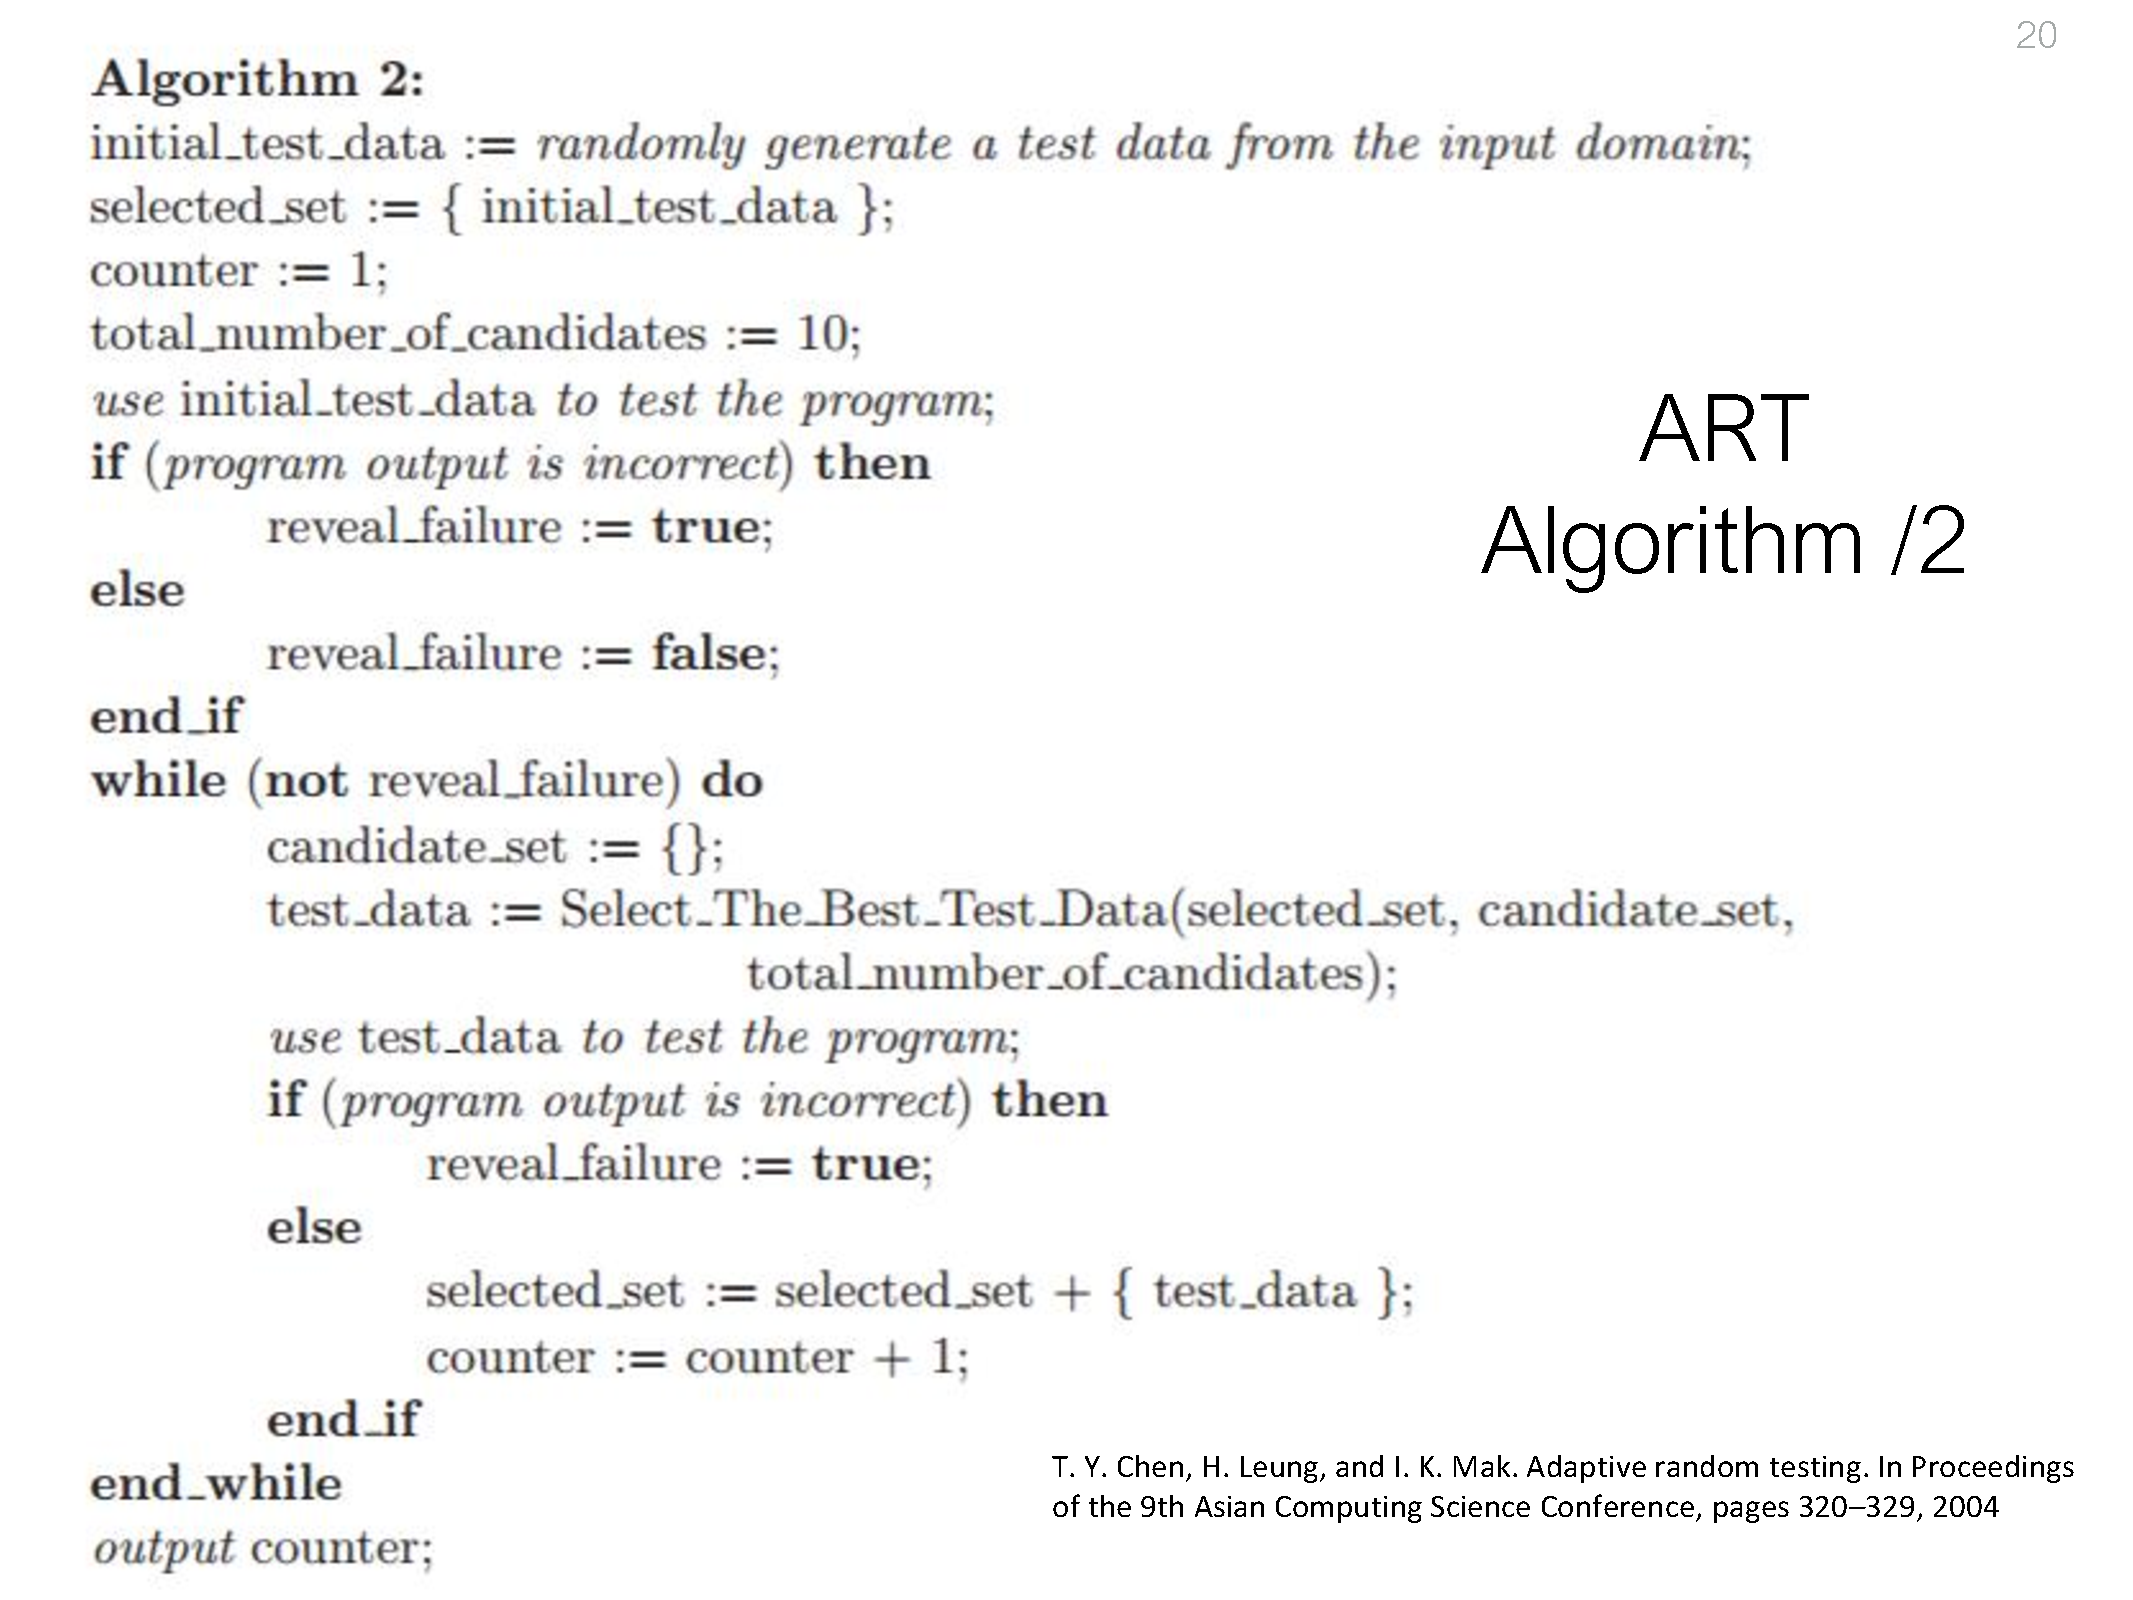
\includegraphics[width=\linewidth]{269.pdf}\\
        \textbf{Random white-box testing}: generate random method invocations \& random parameters\\
        \textbf{Fuzz testing}: random testing technique that involves providing invalid, unexpected or random data as inputs to program, commonly used to discover coding errors \& unknown vulnerabilities in software, OS or networks by inputting massive amounts of random data (fuzz) to system in attempt to make it crash, cost-effective alternative to more systematic testing techniques\\
        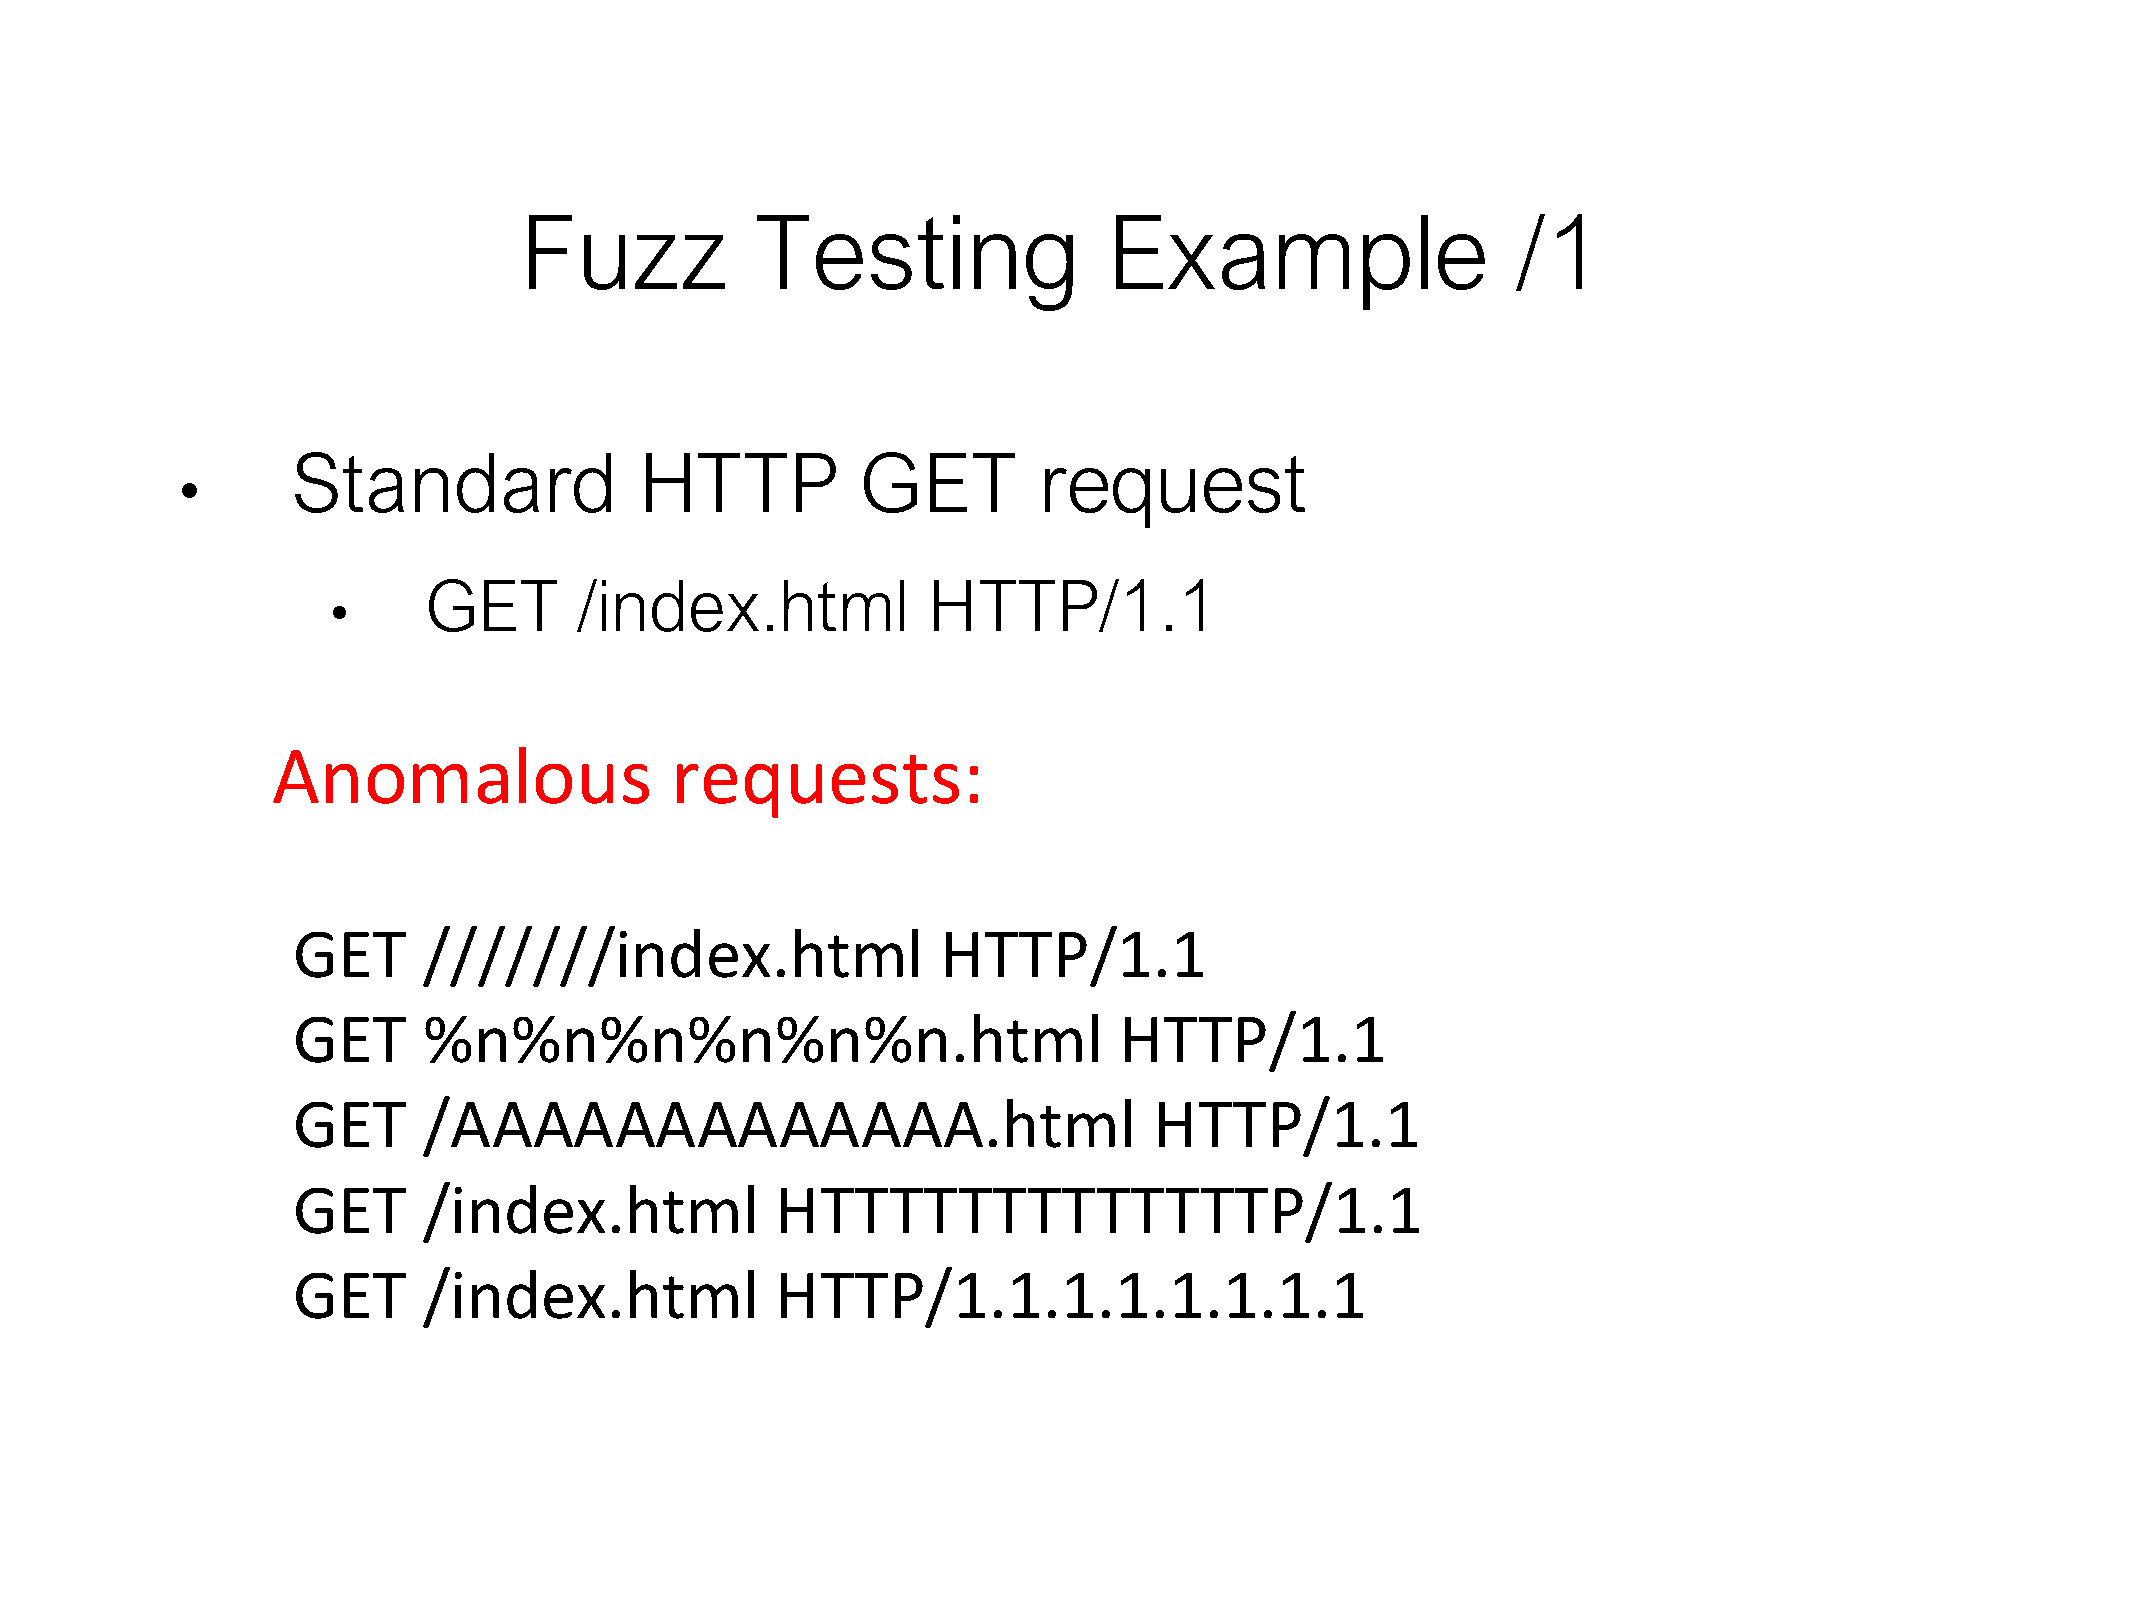
\includegraphics[width=\linewidth]{272.pdf}\\
        \textbf{Ways to generate inputs}:\\
        \textit{Mutation based/dumb fuzzing}: little/no knowledge of input sctructure assumed, anomalies added to existing valid inputs, may be completely random of follow heuristics (remove NL, shift char forward), get inputs, optionally mutate them, feed it to program, record if it crached \& input causing it\\
        \textit{Generation based smart fuzzing}: test cases generated from some description fo format (RFC, docs, etc), anomalies added to each possible spot in inputs, knowledge of protocol should give better results than random fuzzing\\
        \textbf{Fuzzing rules of thumb}: protocol specific knowledge very helpful (generational tends to beat mutation, better specs make better fuzzers), more fuzzers better (each implementation varies different fuzzers find different bugs), the longer it runs the more bugs found, best results come from guiding process (notice where get stuck, use profiling), code coverage useful for guiding process\\
        \textbf{Fuzz testing +/-}: intuituvely simple, but need to figure out how to check the output, corner faults might escape detection, debugging with randomly generated input is challenging\\
        \textbf{Search-based testing}: deem test case generation as search problem, based on random testing \& focus on input domains, use code coverage as guidance (try to generate test case that covers certain code element such as method, statement, branch)\\
        \textbf{Metaheuristic search}:\\
        \textit{Hill climbing}: start from random point, try all neighboring points, go to point with highest value until all neighboring points have value lower than current point, easy to find local optimal\\
        \textit{\textit{Annealing simulation}}: adaptation of hill climbing, has probability to move after reached local peak, probability drops as time goes by\\
        \textit{Genetic algorithm}: simualte process of evolution, start with random points, select number of best points, combine \& mutate points until no more improvements can be made\\
        \textbf{Transform testing to search}: list of random test cases as start point, each test case is point in input domain, use various metaheuristic search algorithms to find test cases, measure how well we have solved the problem (use simeple fitness function, how fat is already covered elements from target code elements, try to make it 0)\\
        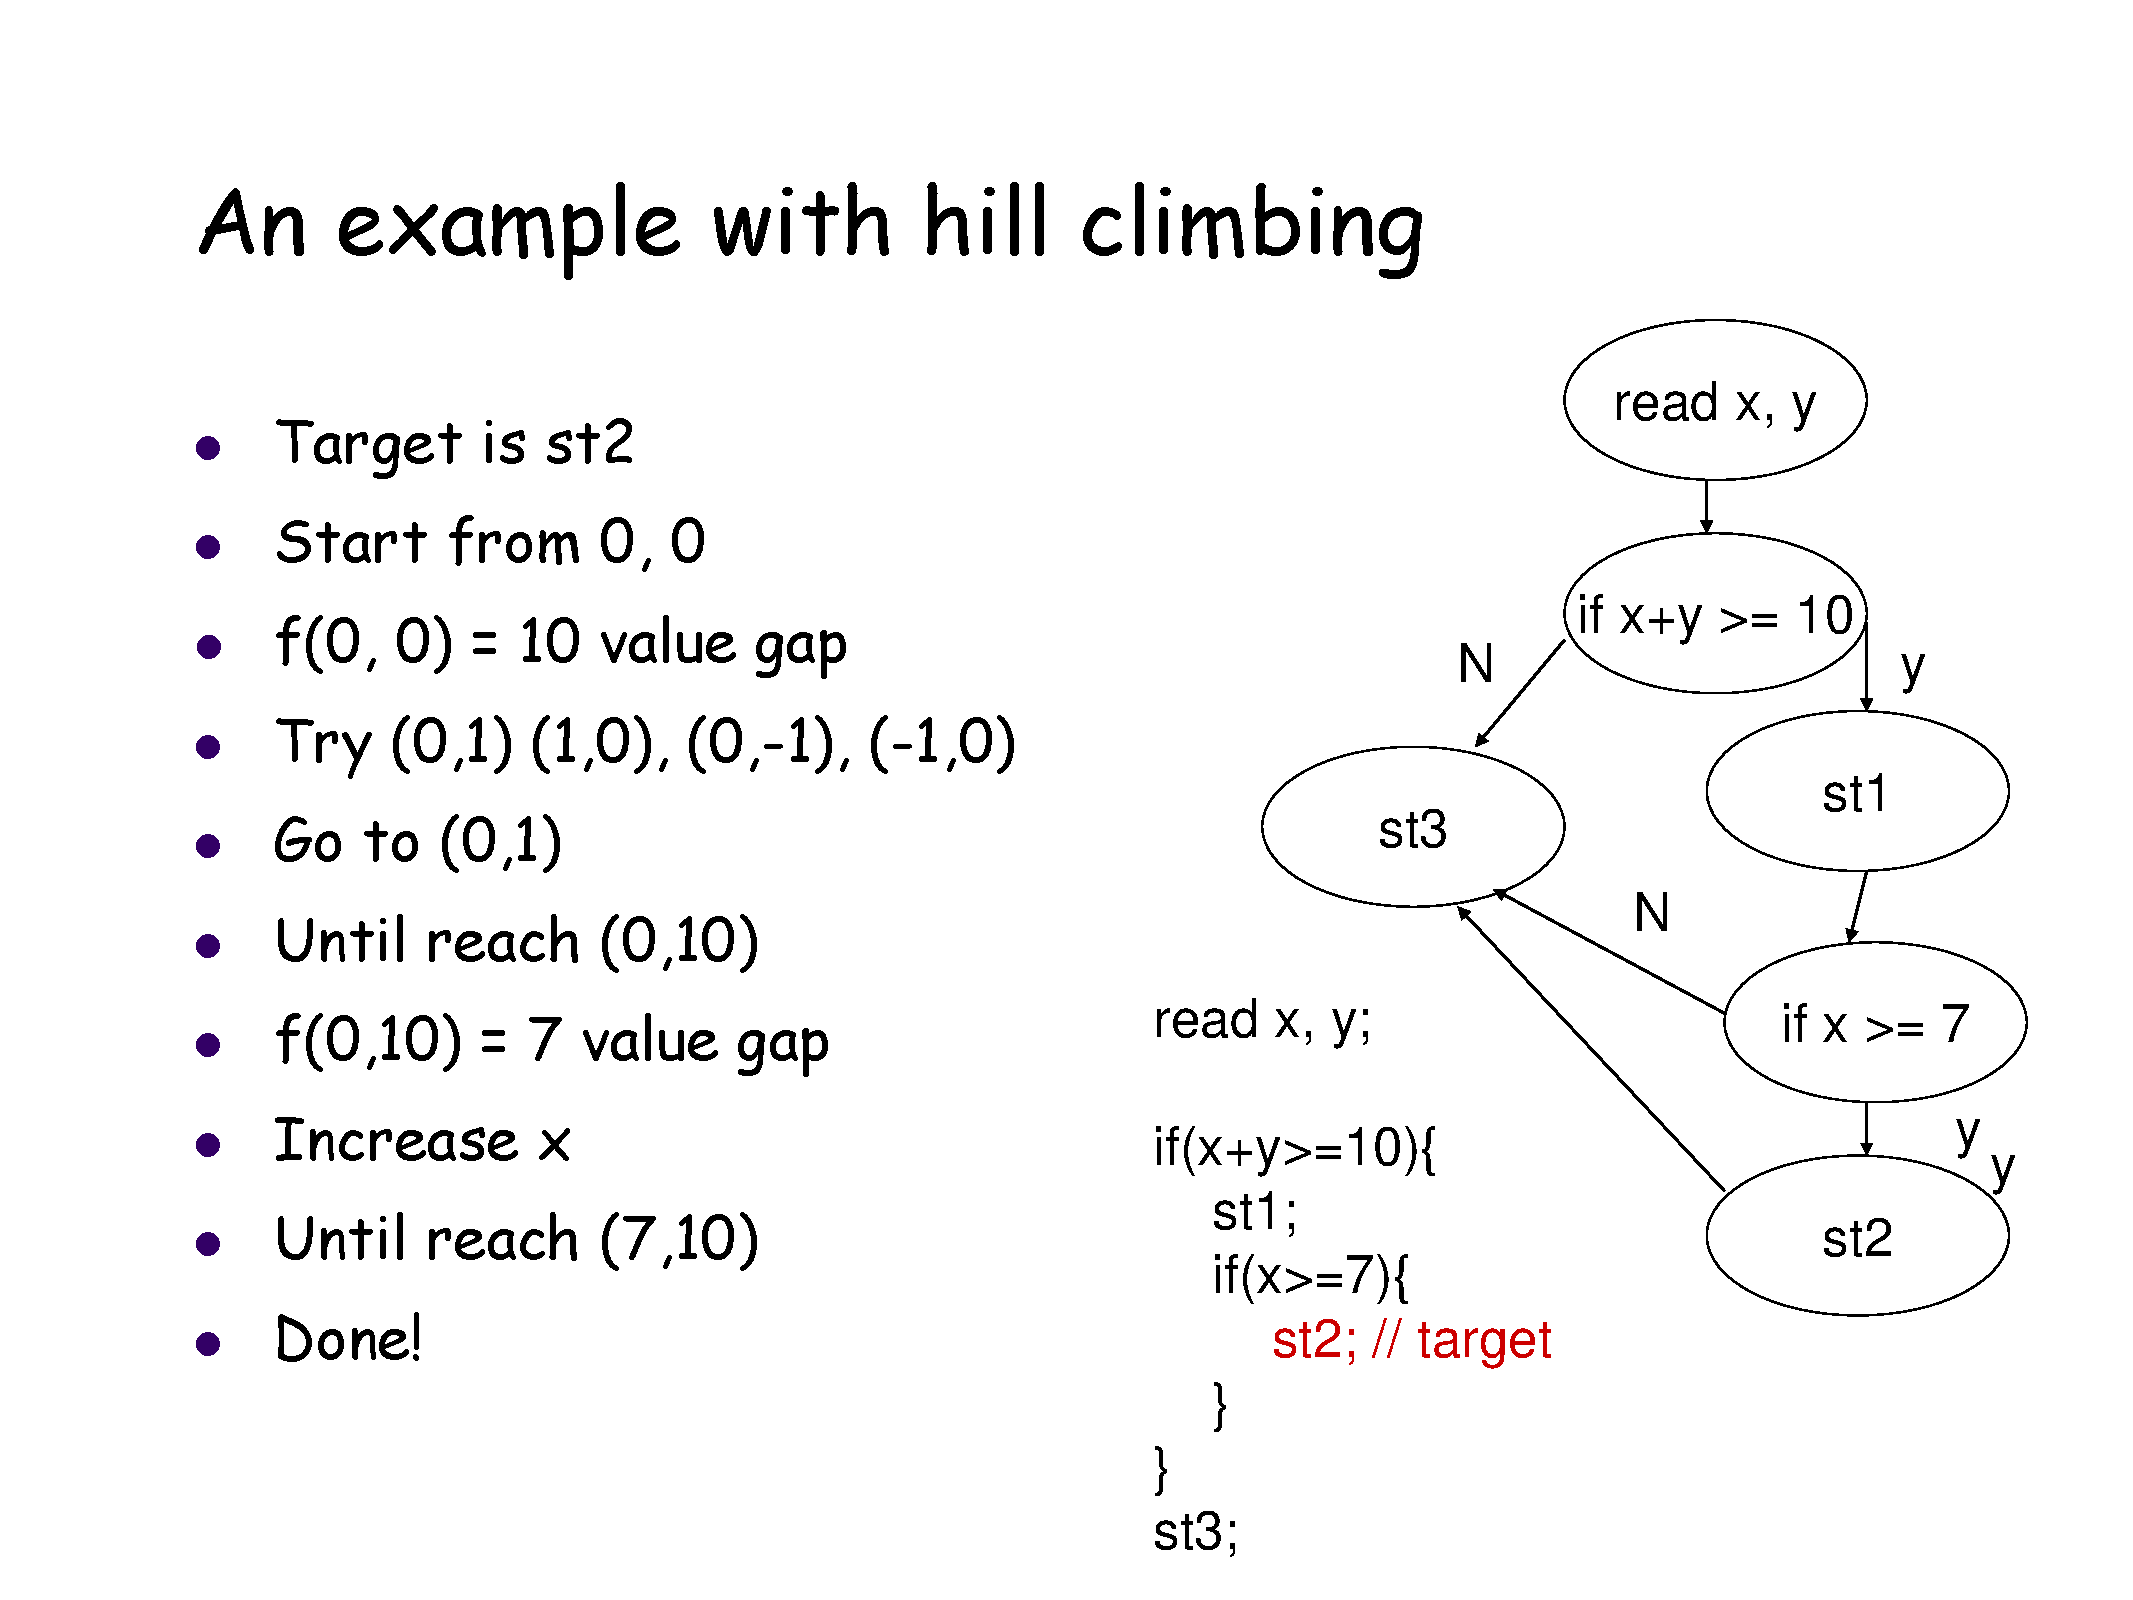
\includegraphics[width=\linewidth]{293.pdf}\\
        \vfill\null\columnbreak\noindent\underline{\textbf{Week 7}}\\
        \textbf{Combinatorial Testing}: instead of all possible combinations generate subset to satisfy some well-defined combination strategies, not every variable contributes to every fault, often fault caused by interactions among few variables, can dramatically reduce number of combinations to be covered but remains very effective in terms of fault detection\\
        \textbf{t-way Interaction}: fault triggered by certain conbination of $t$ input values, simple fault is $t=1$, pairwise is $t=2$\\
        \textbf{Best size for t}: 70\% failures detected by $t=2$, max for fault triggering was $t=6$ for certain interactions (medical devices \& NASA distributed database $t=4$, medical 98\% $t=2$, web server \& browser actually 6)\\
        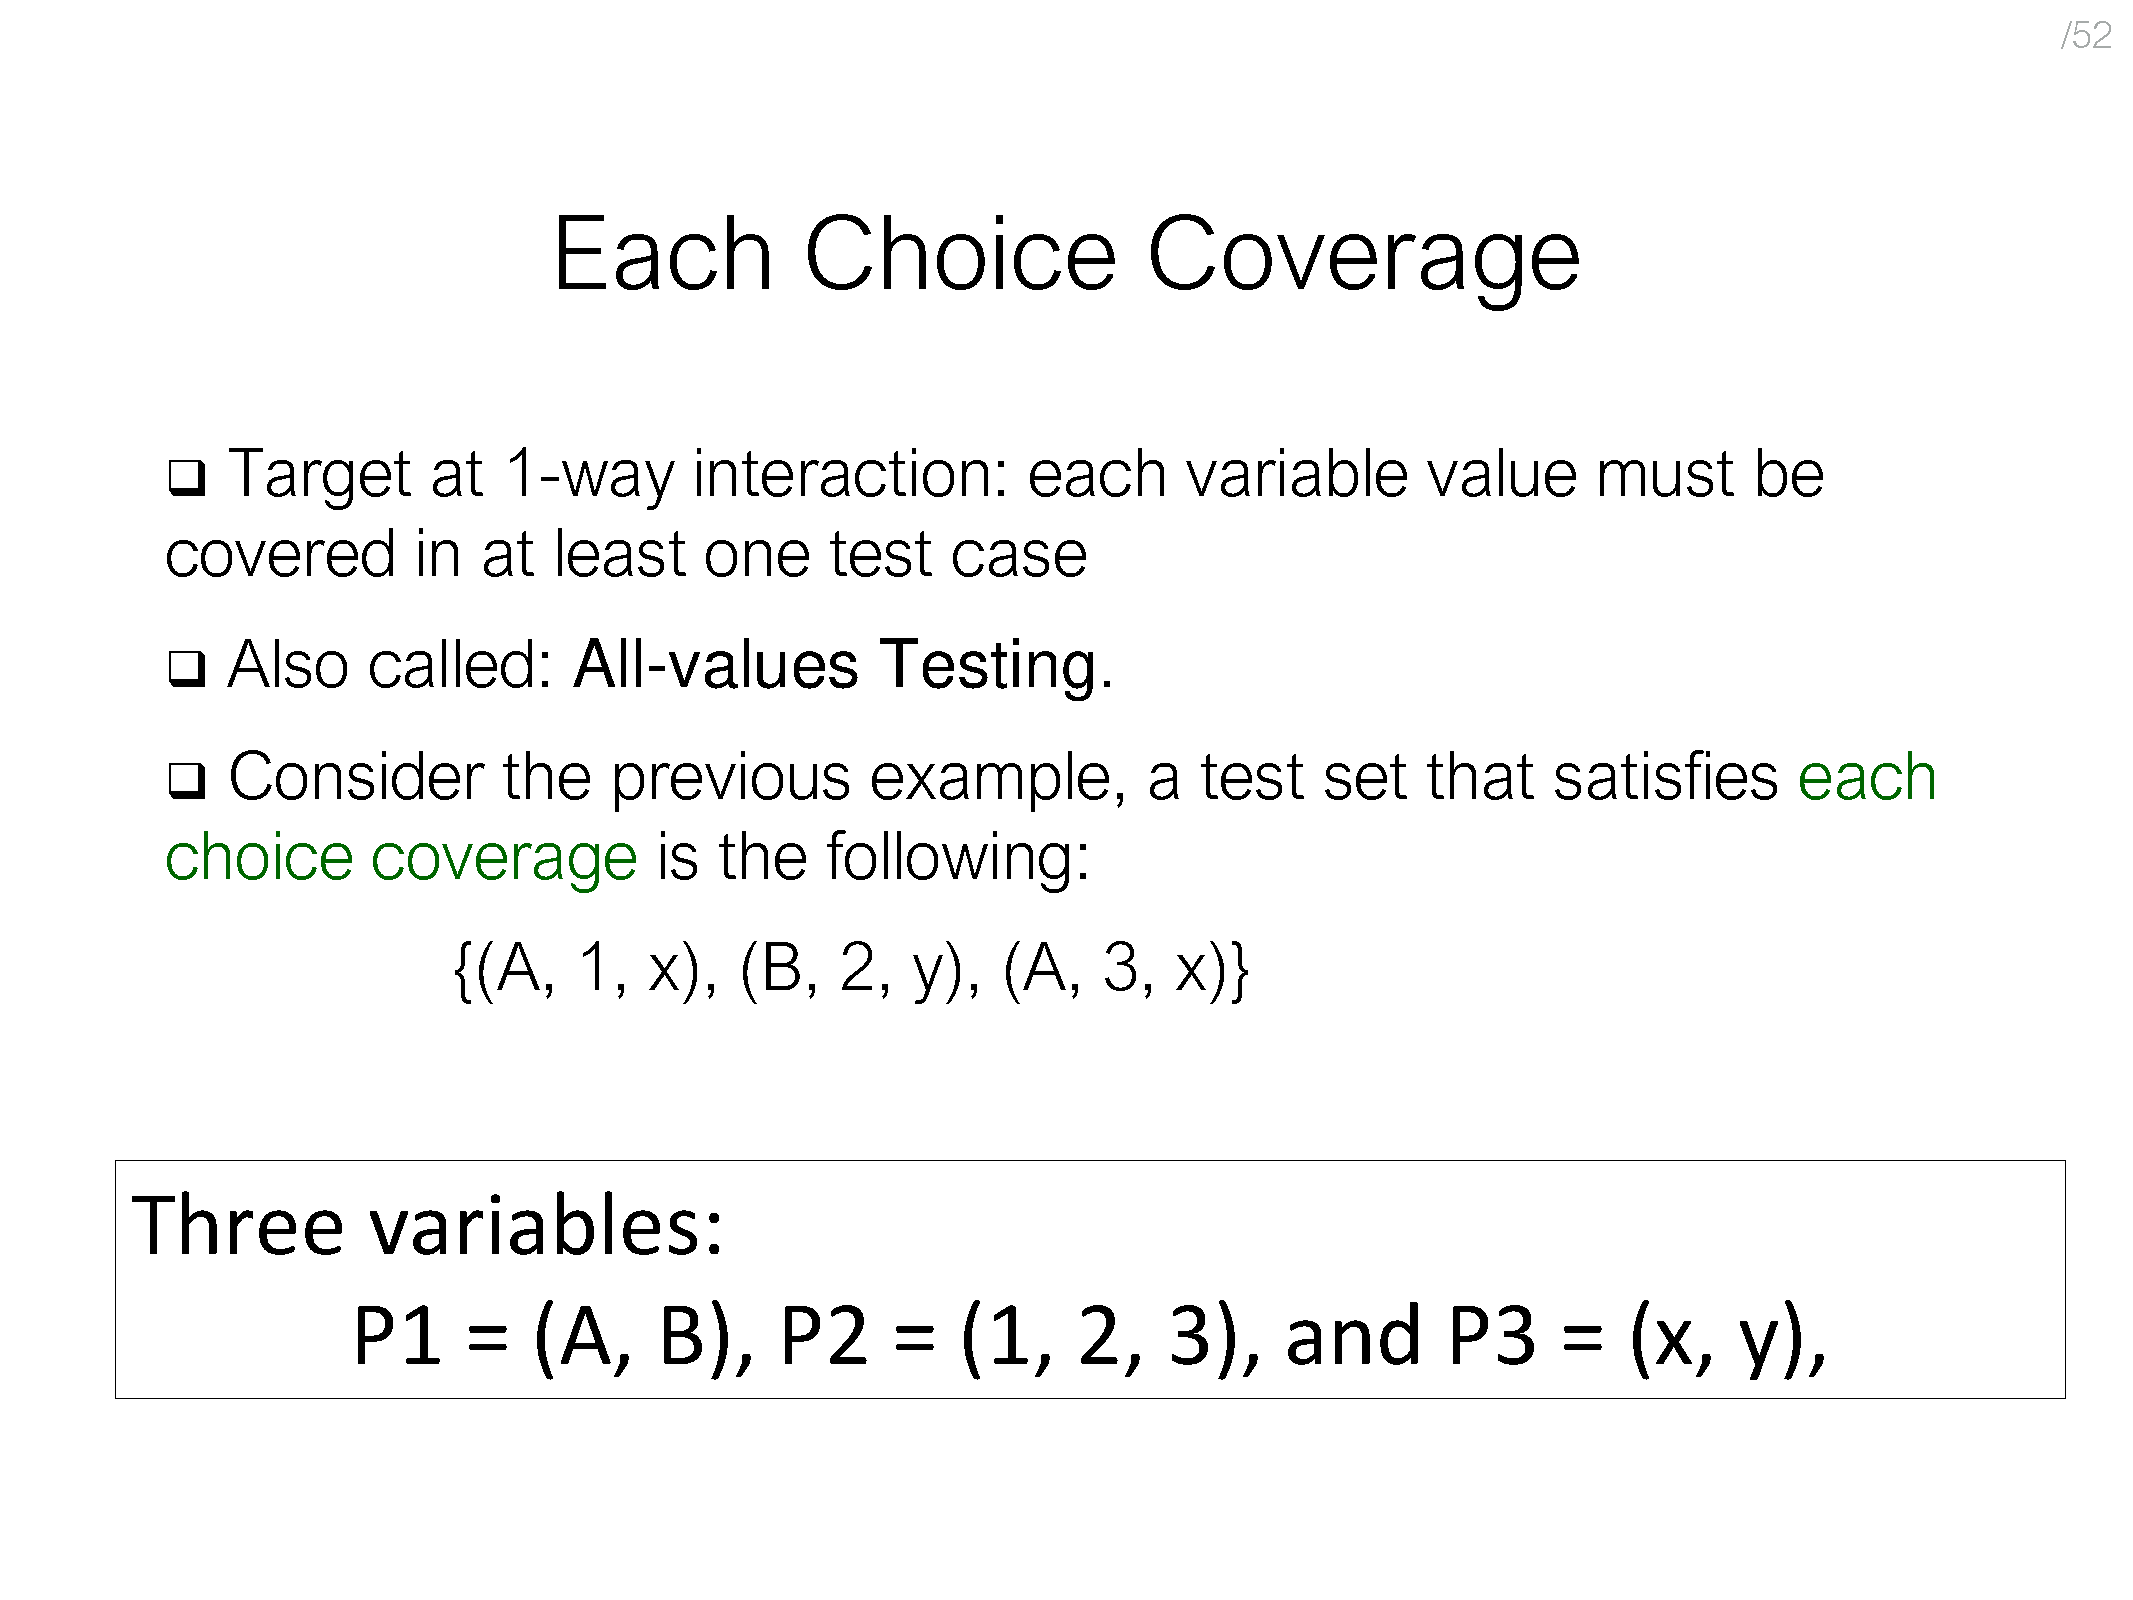
\includegraphics[width=\linewidth]{304.pdf}\\
        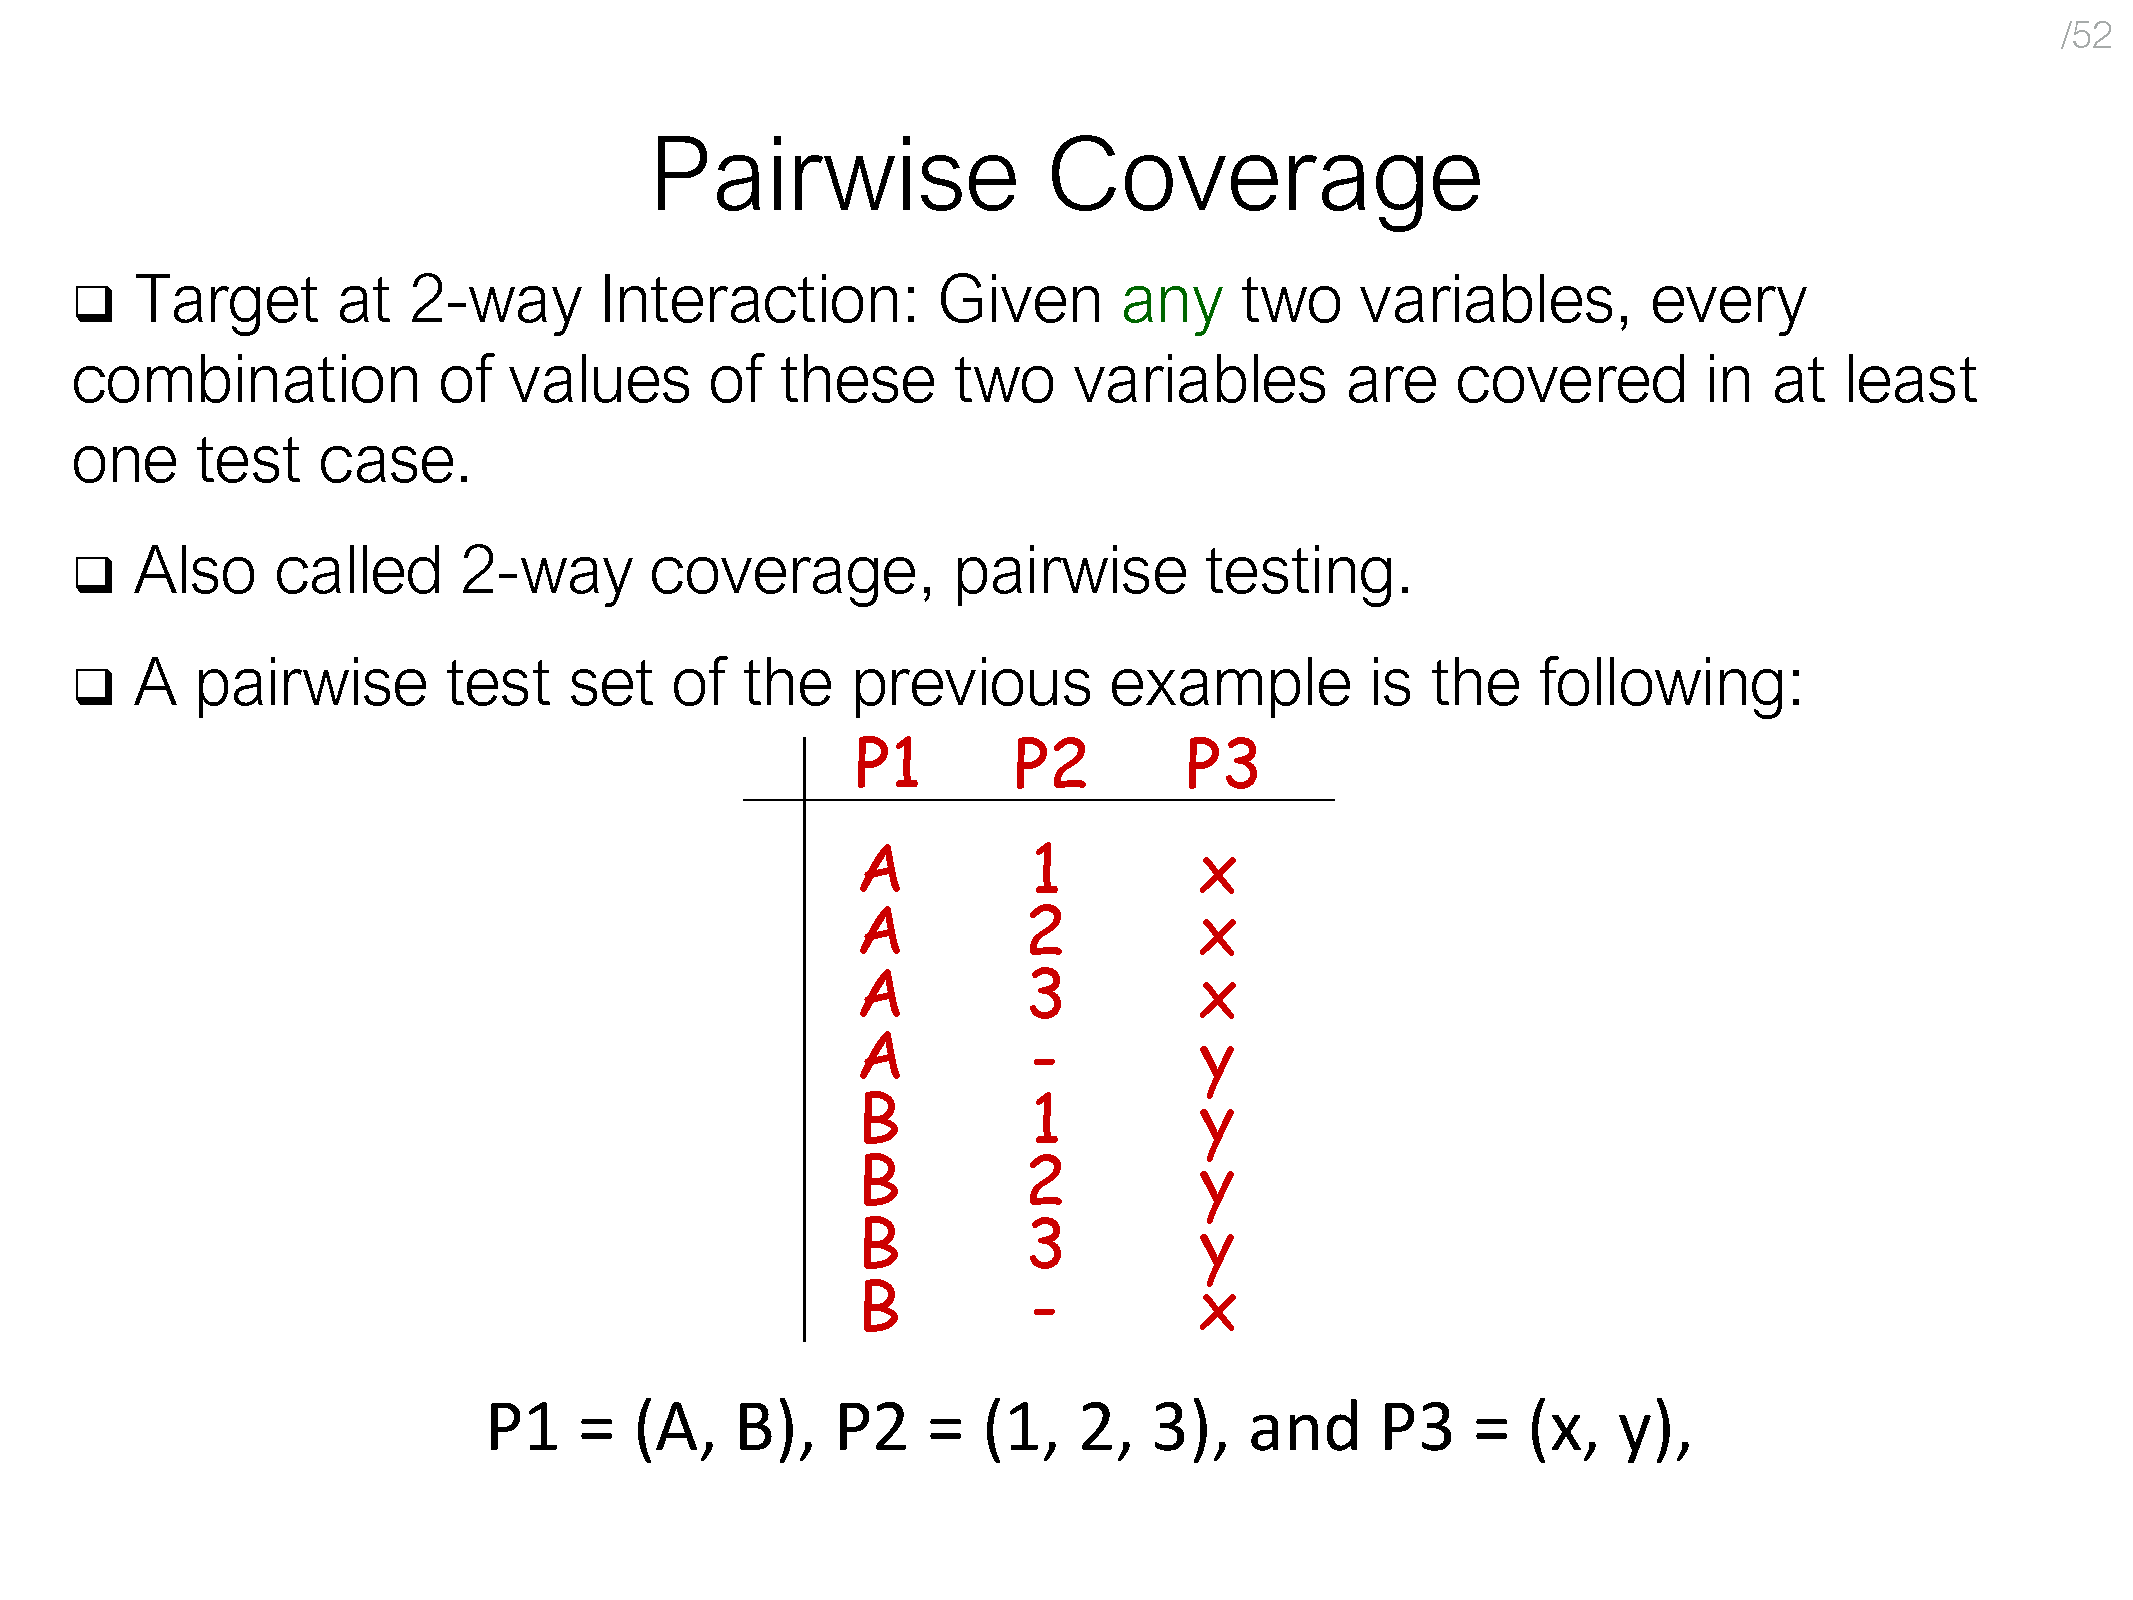
\includegraphics[width=\linewidth]{305.pdf}\\
        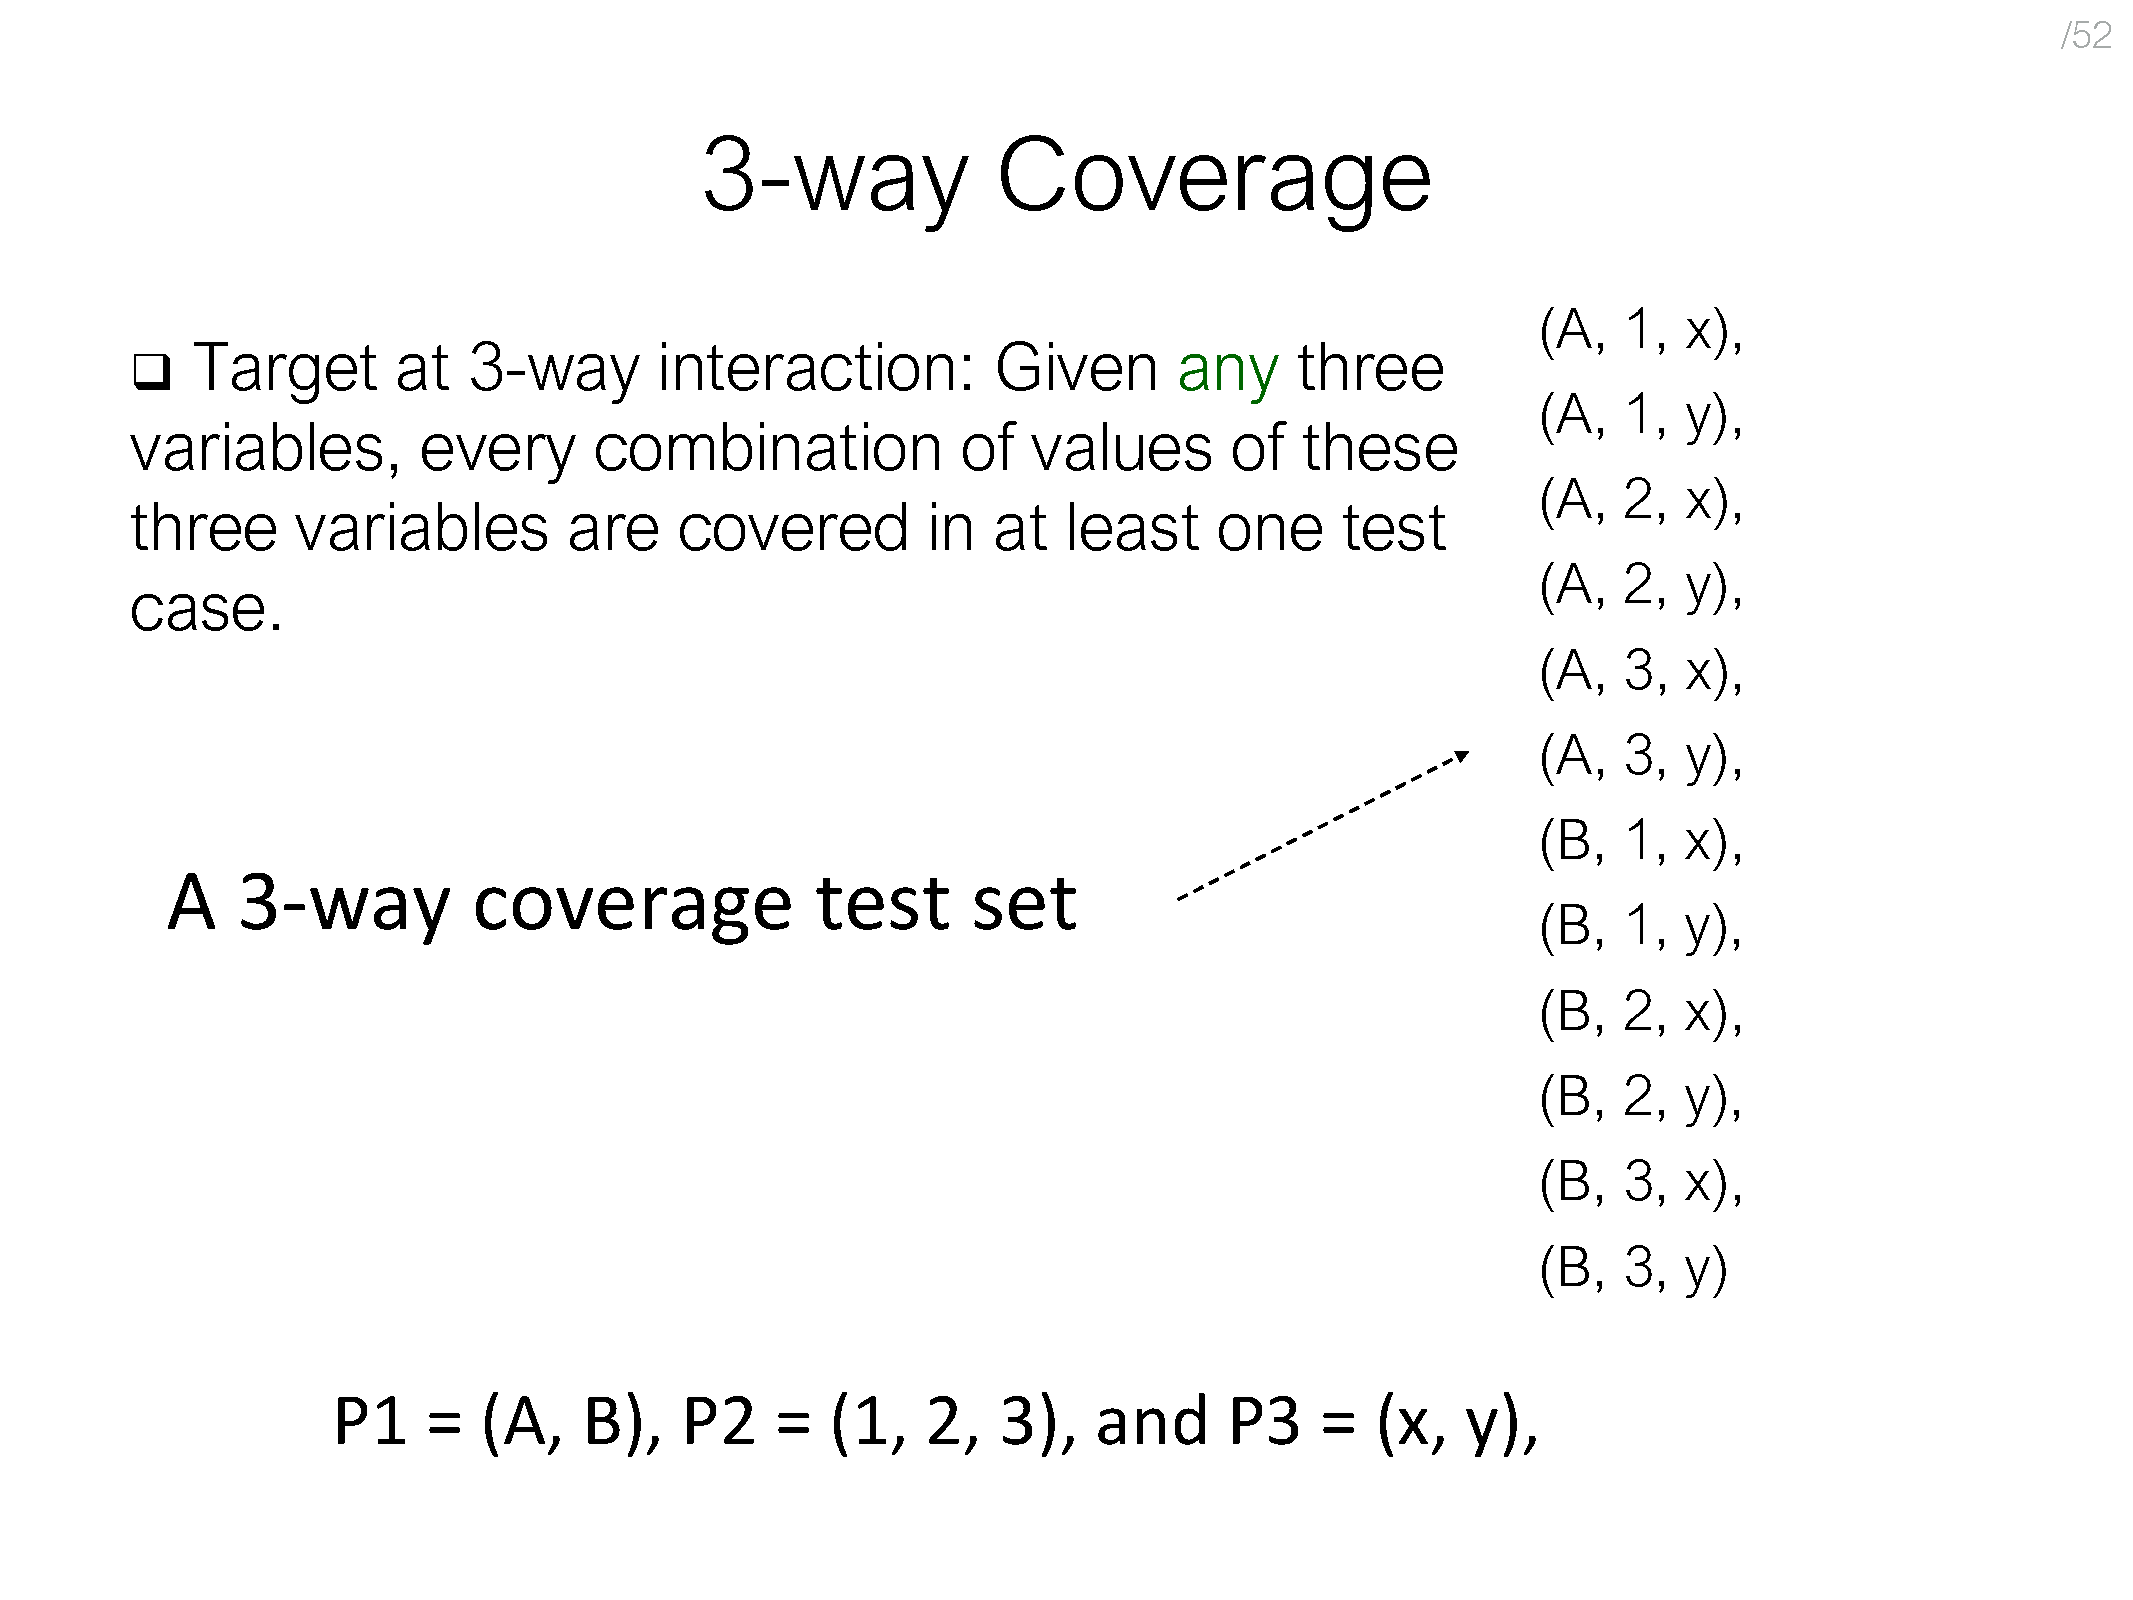
\includegraphics[width=\linewidth]{306.pdf}\\
        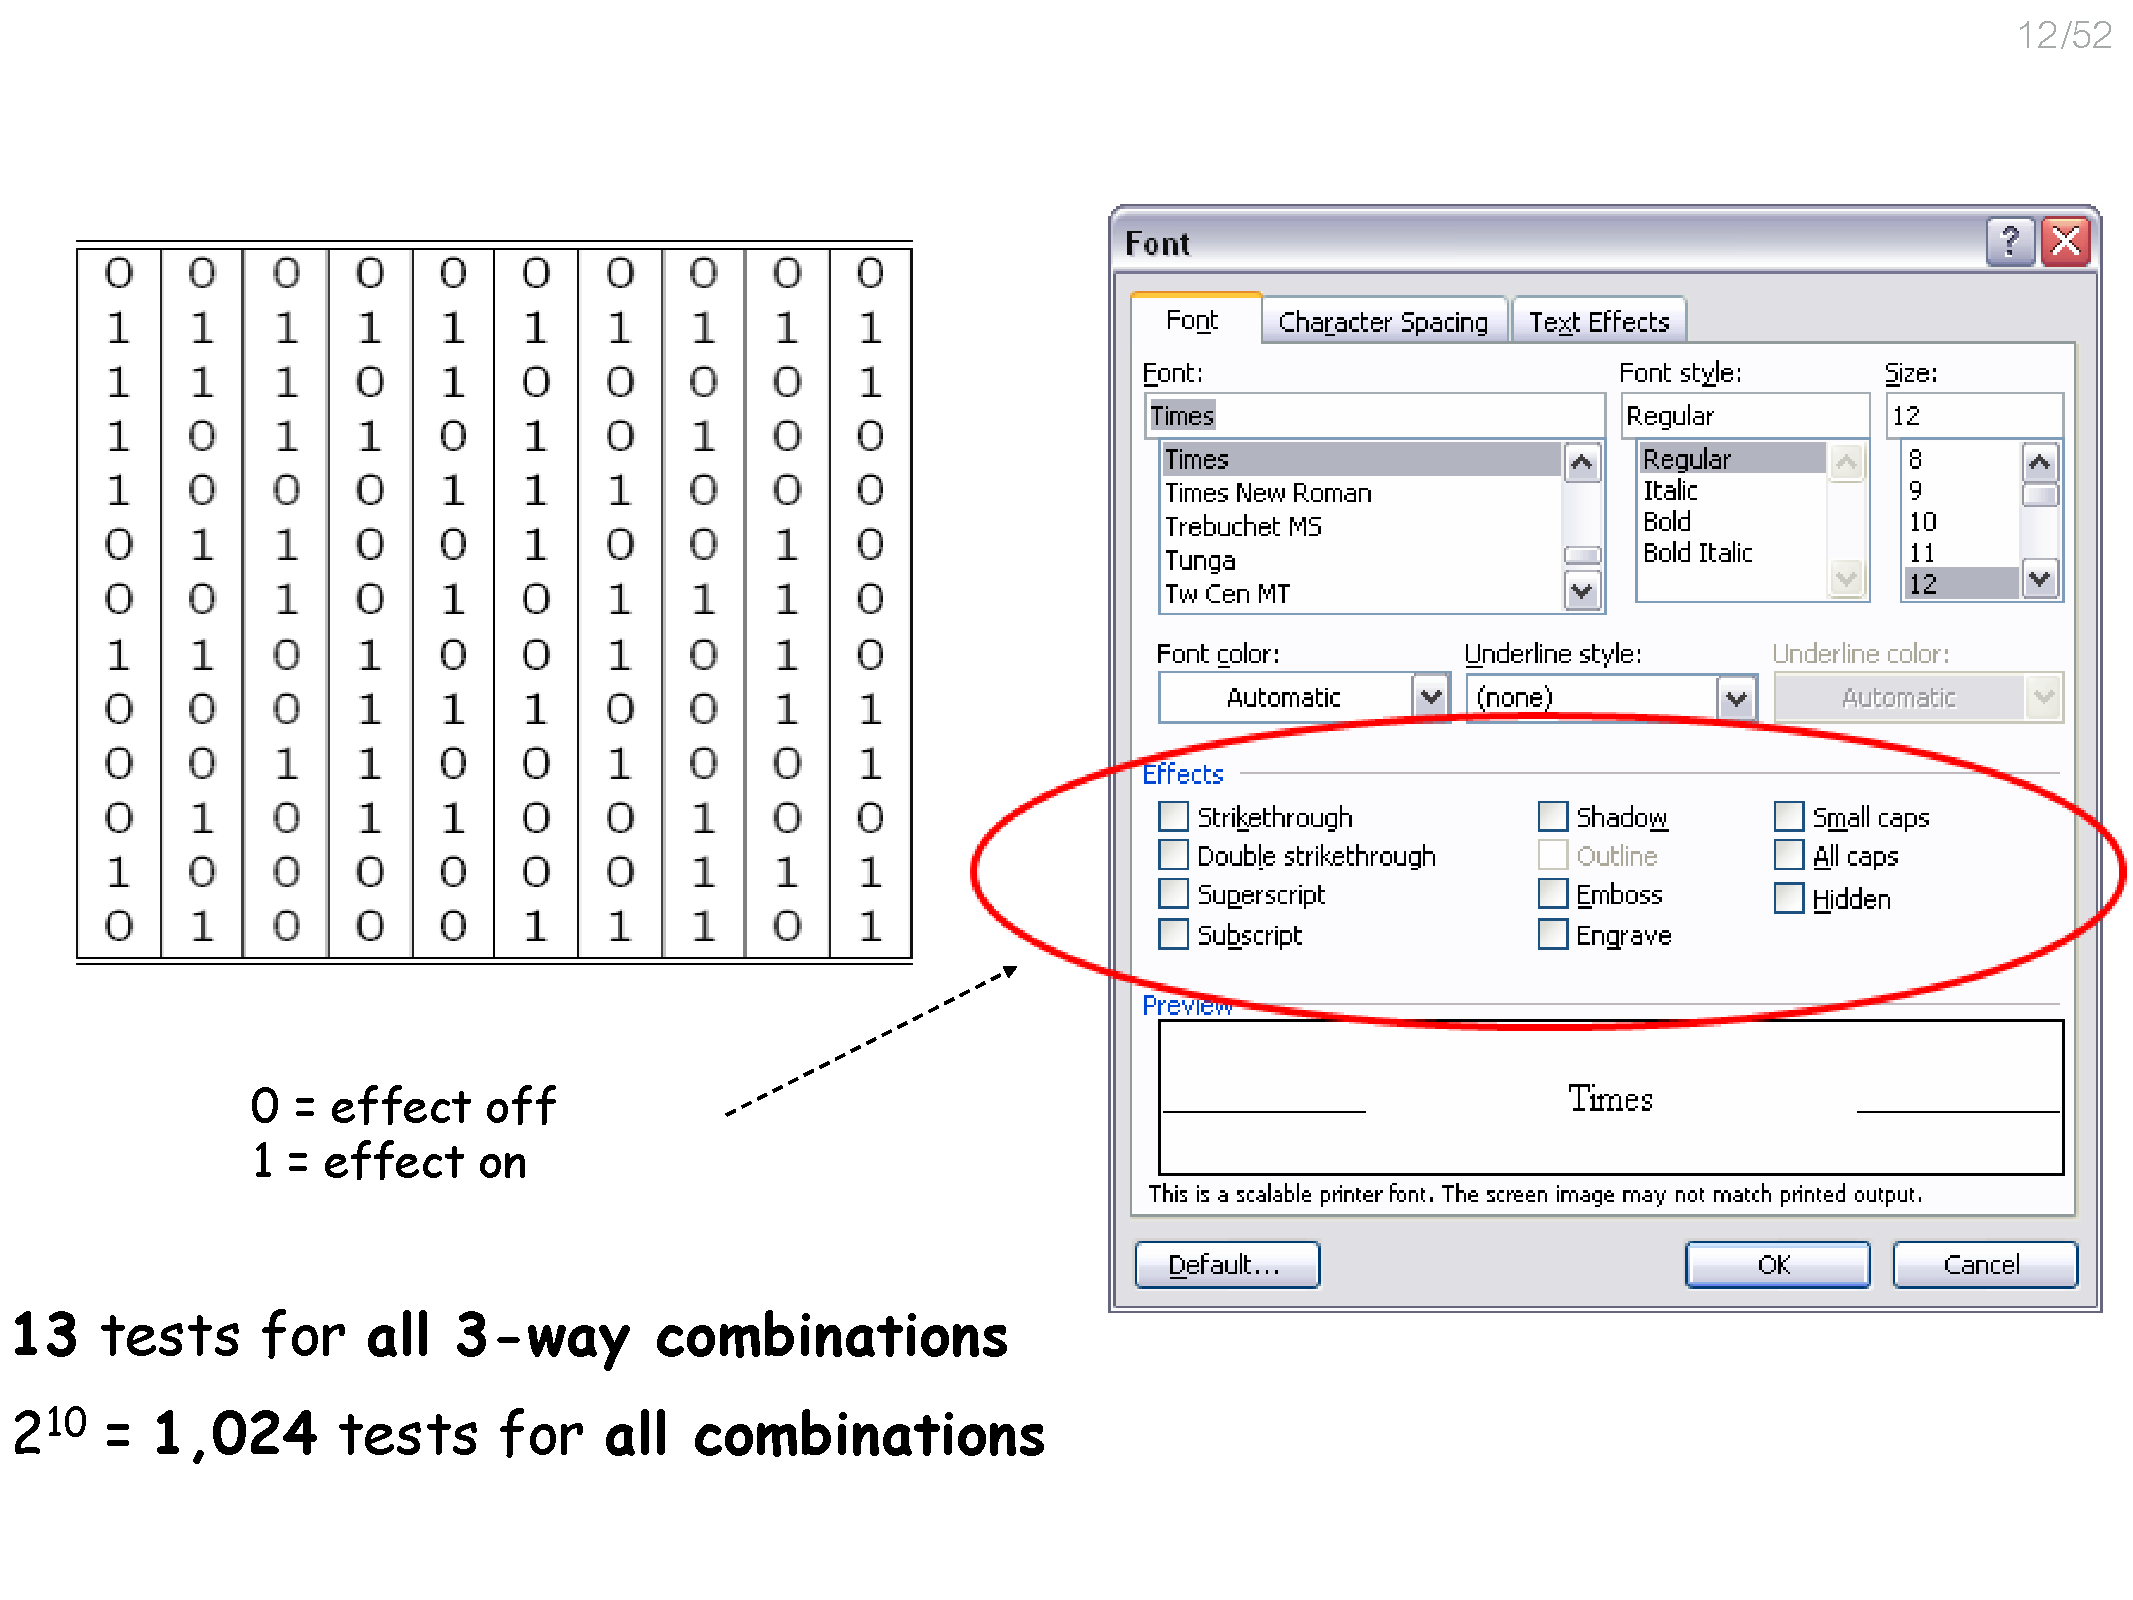
\includegraphics[width=\linewidth]{308.pdf}\\
        \textbf{Problem formulation for combinatorial testing}: for fixed $t$, $v$ \& $k$ costruct smallest $t$-way covering array\\
        \textbf{t-way covering array}: for every $t$ parameters all value combinations must appear at least once in covering array, $k$ is number of variables, $v$ is number of possible variables each variable can take, generating minimum is NP-complete\\
        \textbf{Mathematical approach}: can yield smallest possible covering arrays (orthogonal array)\\
        \textbf{Computational approach}: can be applied to any types of covering arrays, but consume more time (random, greedy, search based approaches)\\
        \textbf{In-Parameter-Order}: test generation strategy for combinatorial testing, first generate pairwise set for first 2 parameters, then for first three, so on, pairwise set for first $n$ parameters built by extending test set for first $n-1$ parameters\\
        \textbf{Horizontal growth}: extend each existing test case by adding one value of new parameter\\
        \textbf{Vertical growth}: adds new tests if necessary\\
        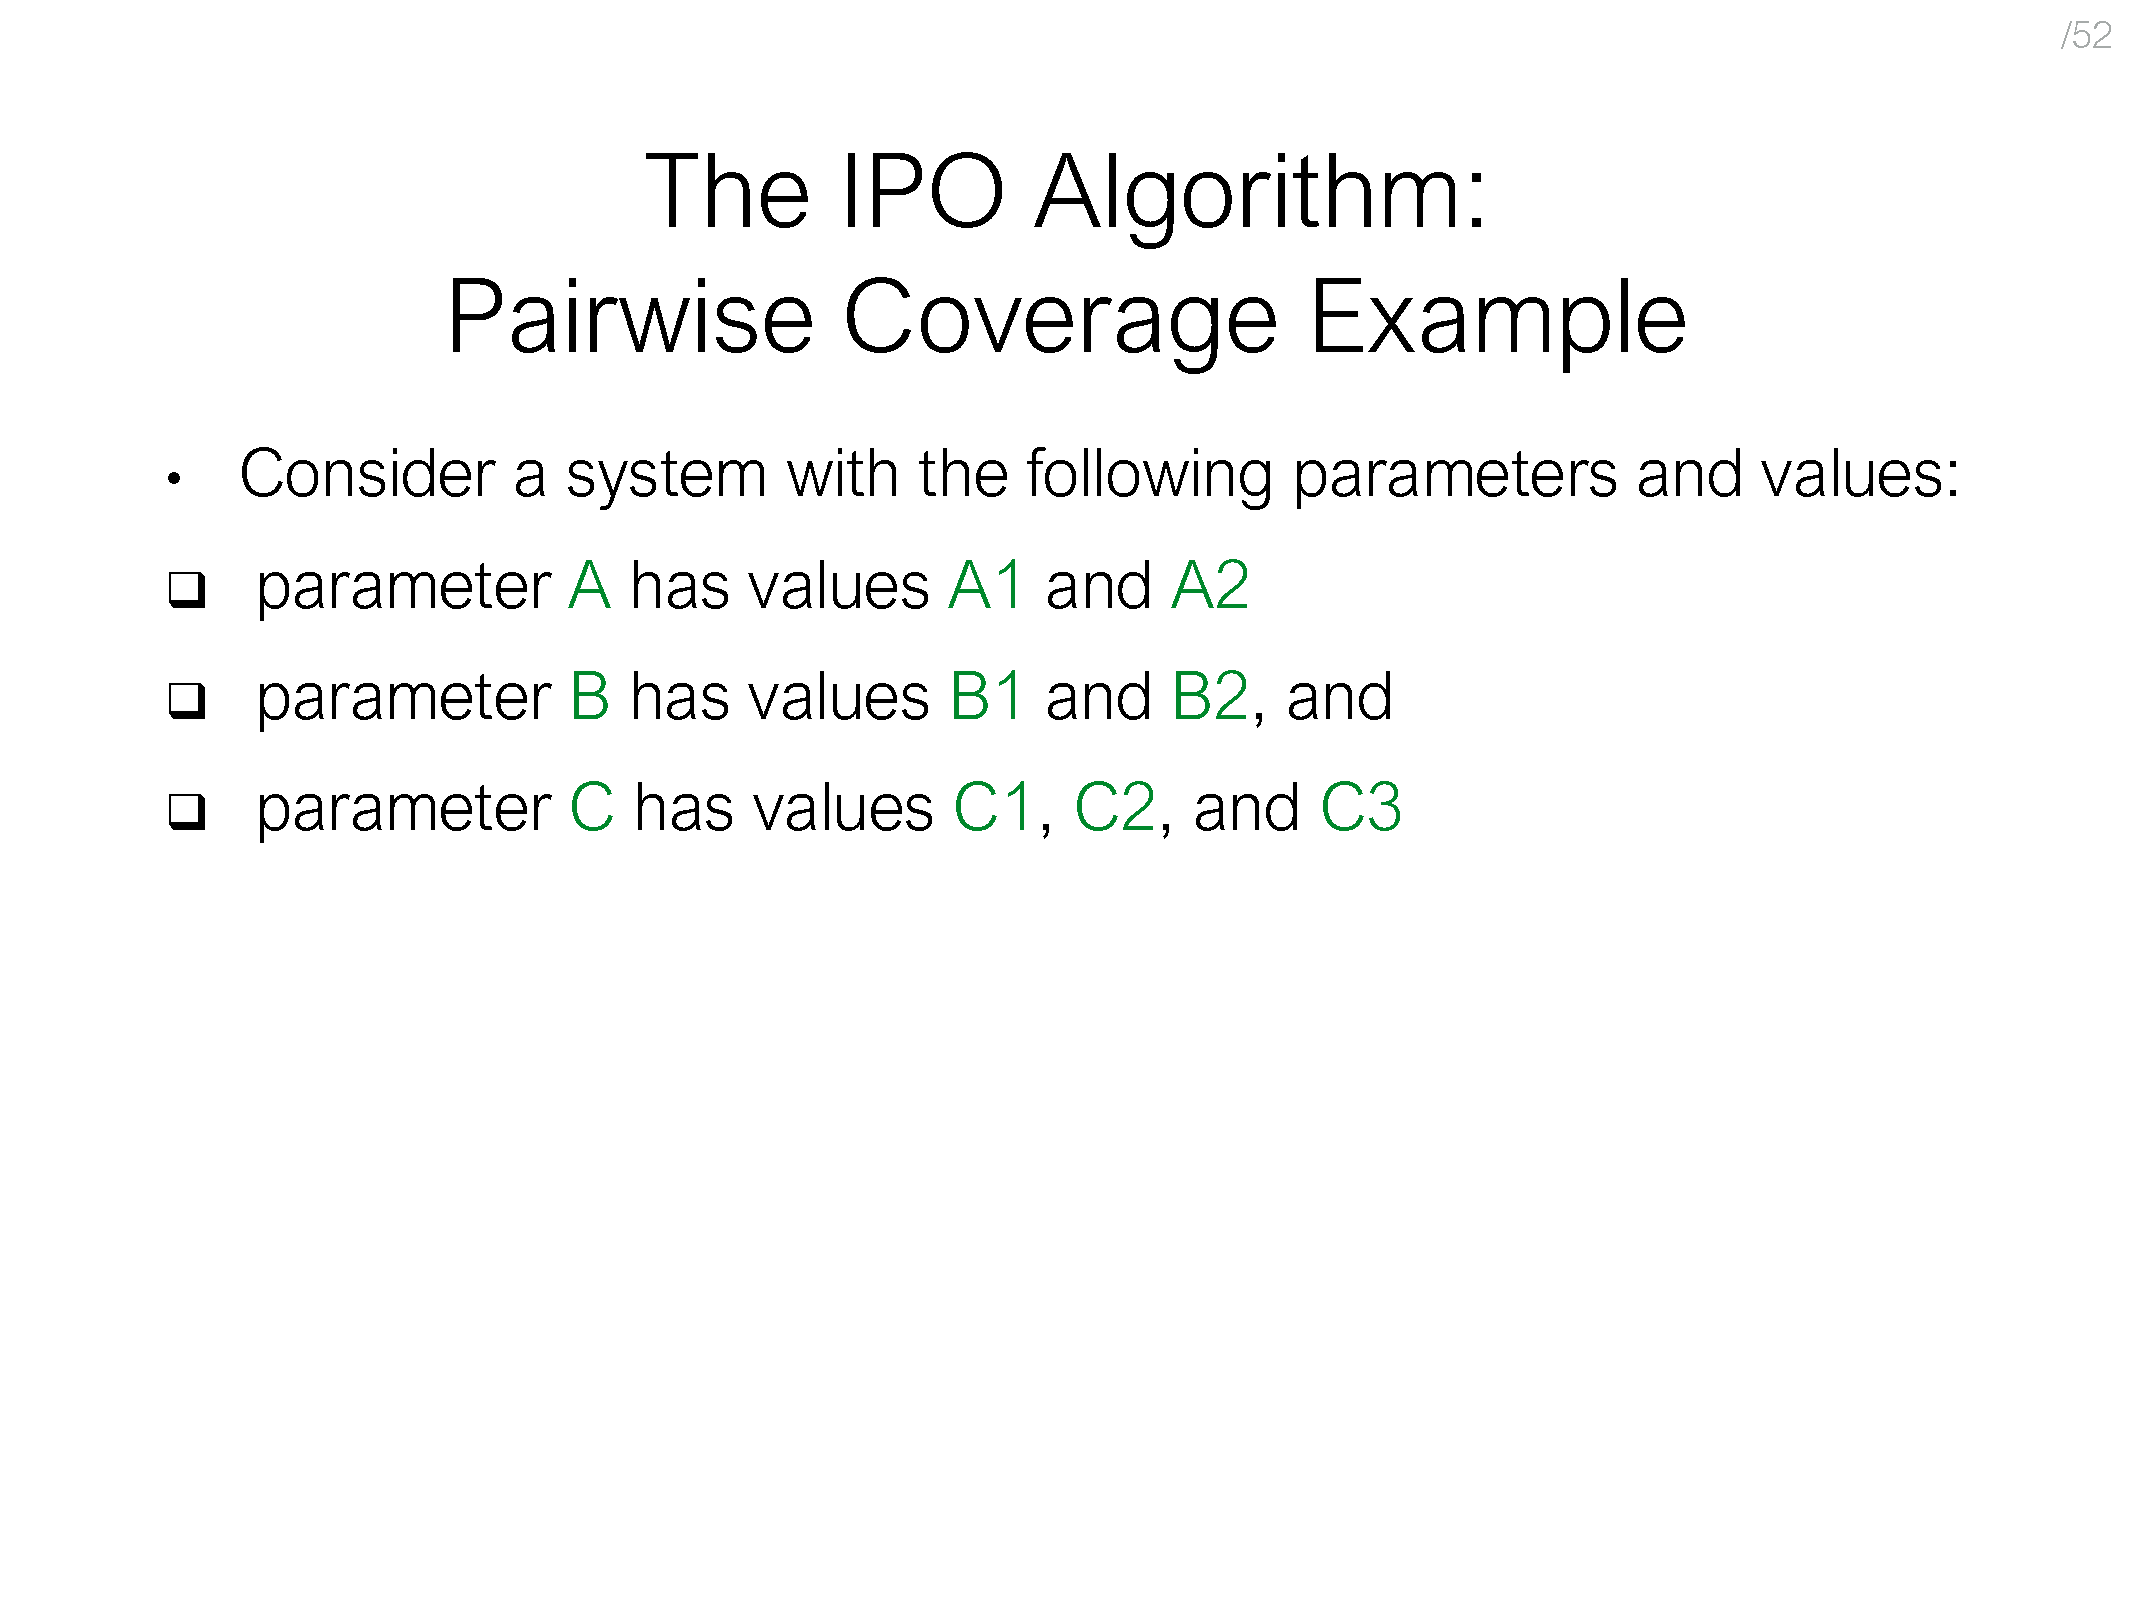
\includegraphics[width=\linewidth]{319.pdf}\\
        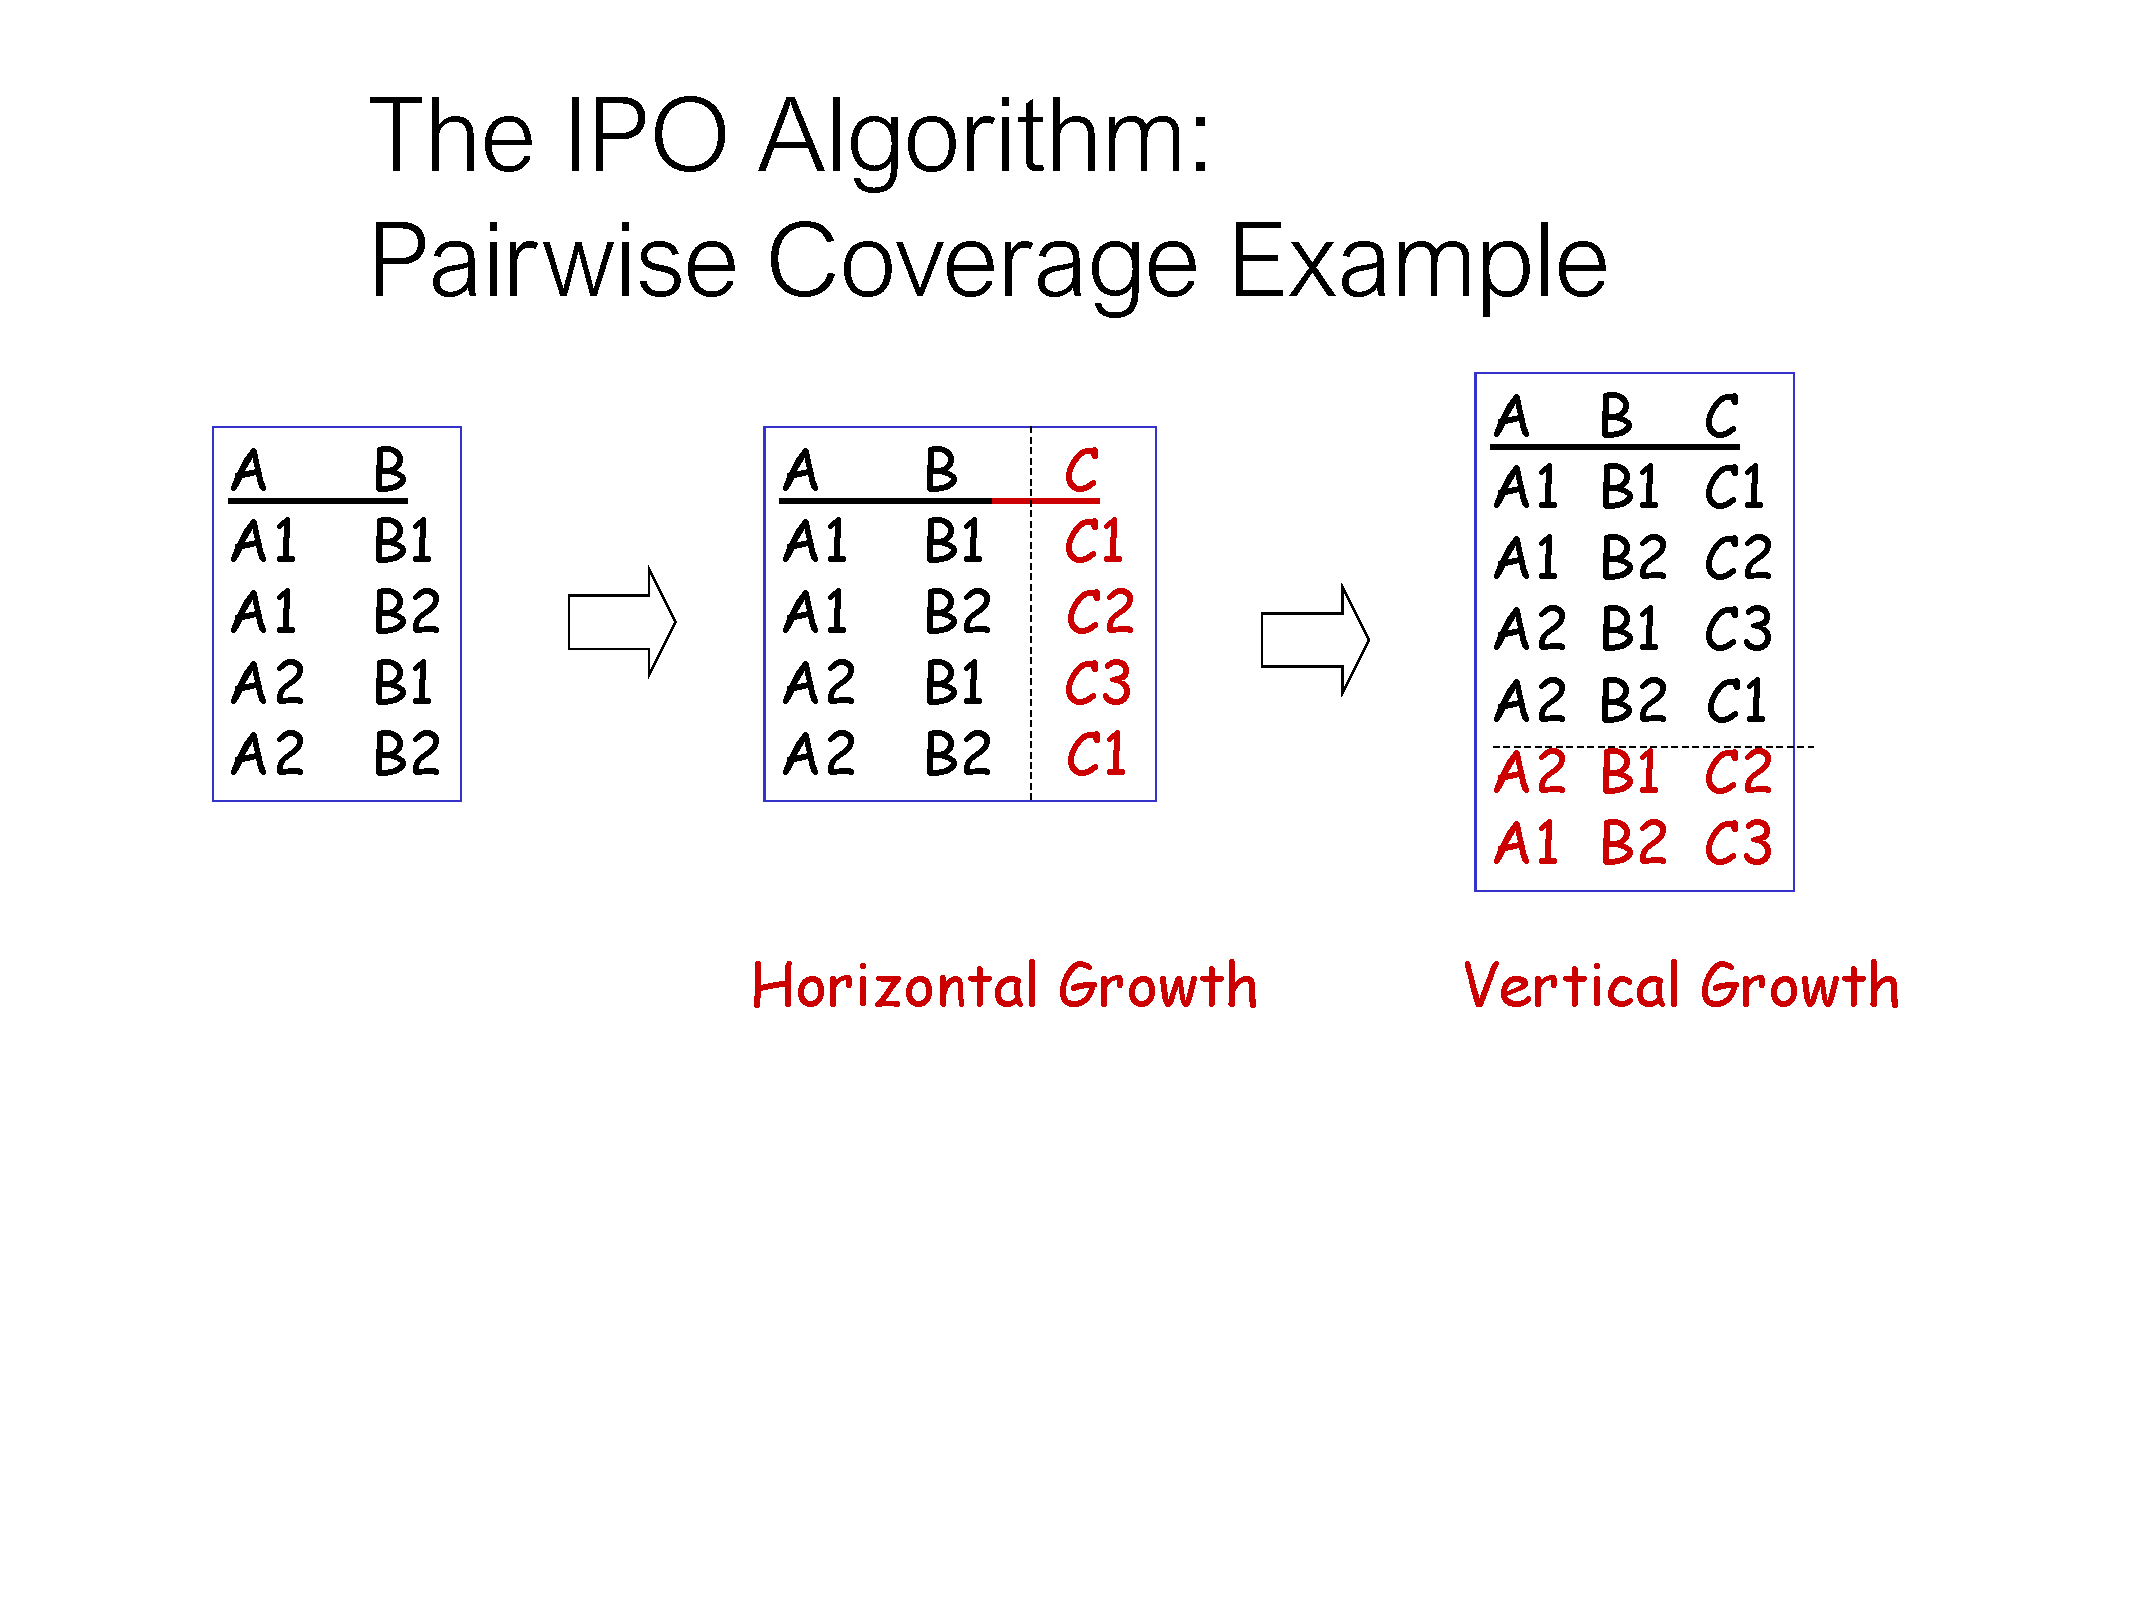
\includegraphics[width=\linewidth]{320.pdf}\\
        \textbf{Non-functional testing}:\\
        \textit{Performance}: how system performs in terms of responsiveness \& stability under particular workload, evaluates system performance under normal \& heavy usage, considers scalability \& load (test ability to handle real-world volumes typically by generating many user access simulations)\\
        \textit{Stress}: test reliability under unexpected or rare workloads, consists of subjecting the system to varying \& max loads to evaluate resulting performance, can be automated\\
        \textit{Security}: concerned mainly with security-related aspects of software, primary concern when communicating \& conducting business especially sensitive \& business critical transactions over Internet, regardless whether app requires user to enter password for access still must check for internet threats\\
        \textit{Usability}: concerned mainly with the use of the software, assess user friendliness \& suitability by gathering info about how users interact with site, study what user actually does\\
        \textbf{Stress testing tool report}: number of requests, transactions, KBps, round trip time (from user making request to receiving result), number of concurrent connection, performance degradation, types of visitors to site \& number, CPU \& memory use of app server\\
        \textbf{Top 2 Web App Security Risks}:\\
        \textit{Injection}: SQL, OS, LDAP, occur whe untrusted data sent to interpreter as part of command/query\\
        \textit{Cross Site Scripting}: occur whenever app takes untrusted data \& send to web browser without proper validation \& escaping\\
        \textbf{Injection Protectiom}: validate input (careful with special characters, whitelist, validate length, type, syntax), avoid use of interpreter (use stored procedures), otherwise use safe APIs (strongly typed parameterised queries, such as PreparedStatement), use Object Relational Manager\\
        \textbf{XSS Protection}: appropriate encoding of all output data (HTML/XML depending on output mechanism, encode all characters other than very limited subset, specify character encoding)\\
        \textbf{Usability Testing Steps}: identify website purpose, identify intended users, define tests \& conduct usability testing, analyze acquired info\\
        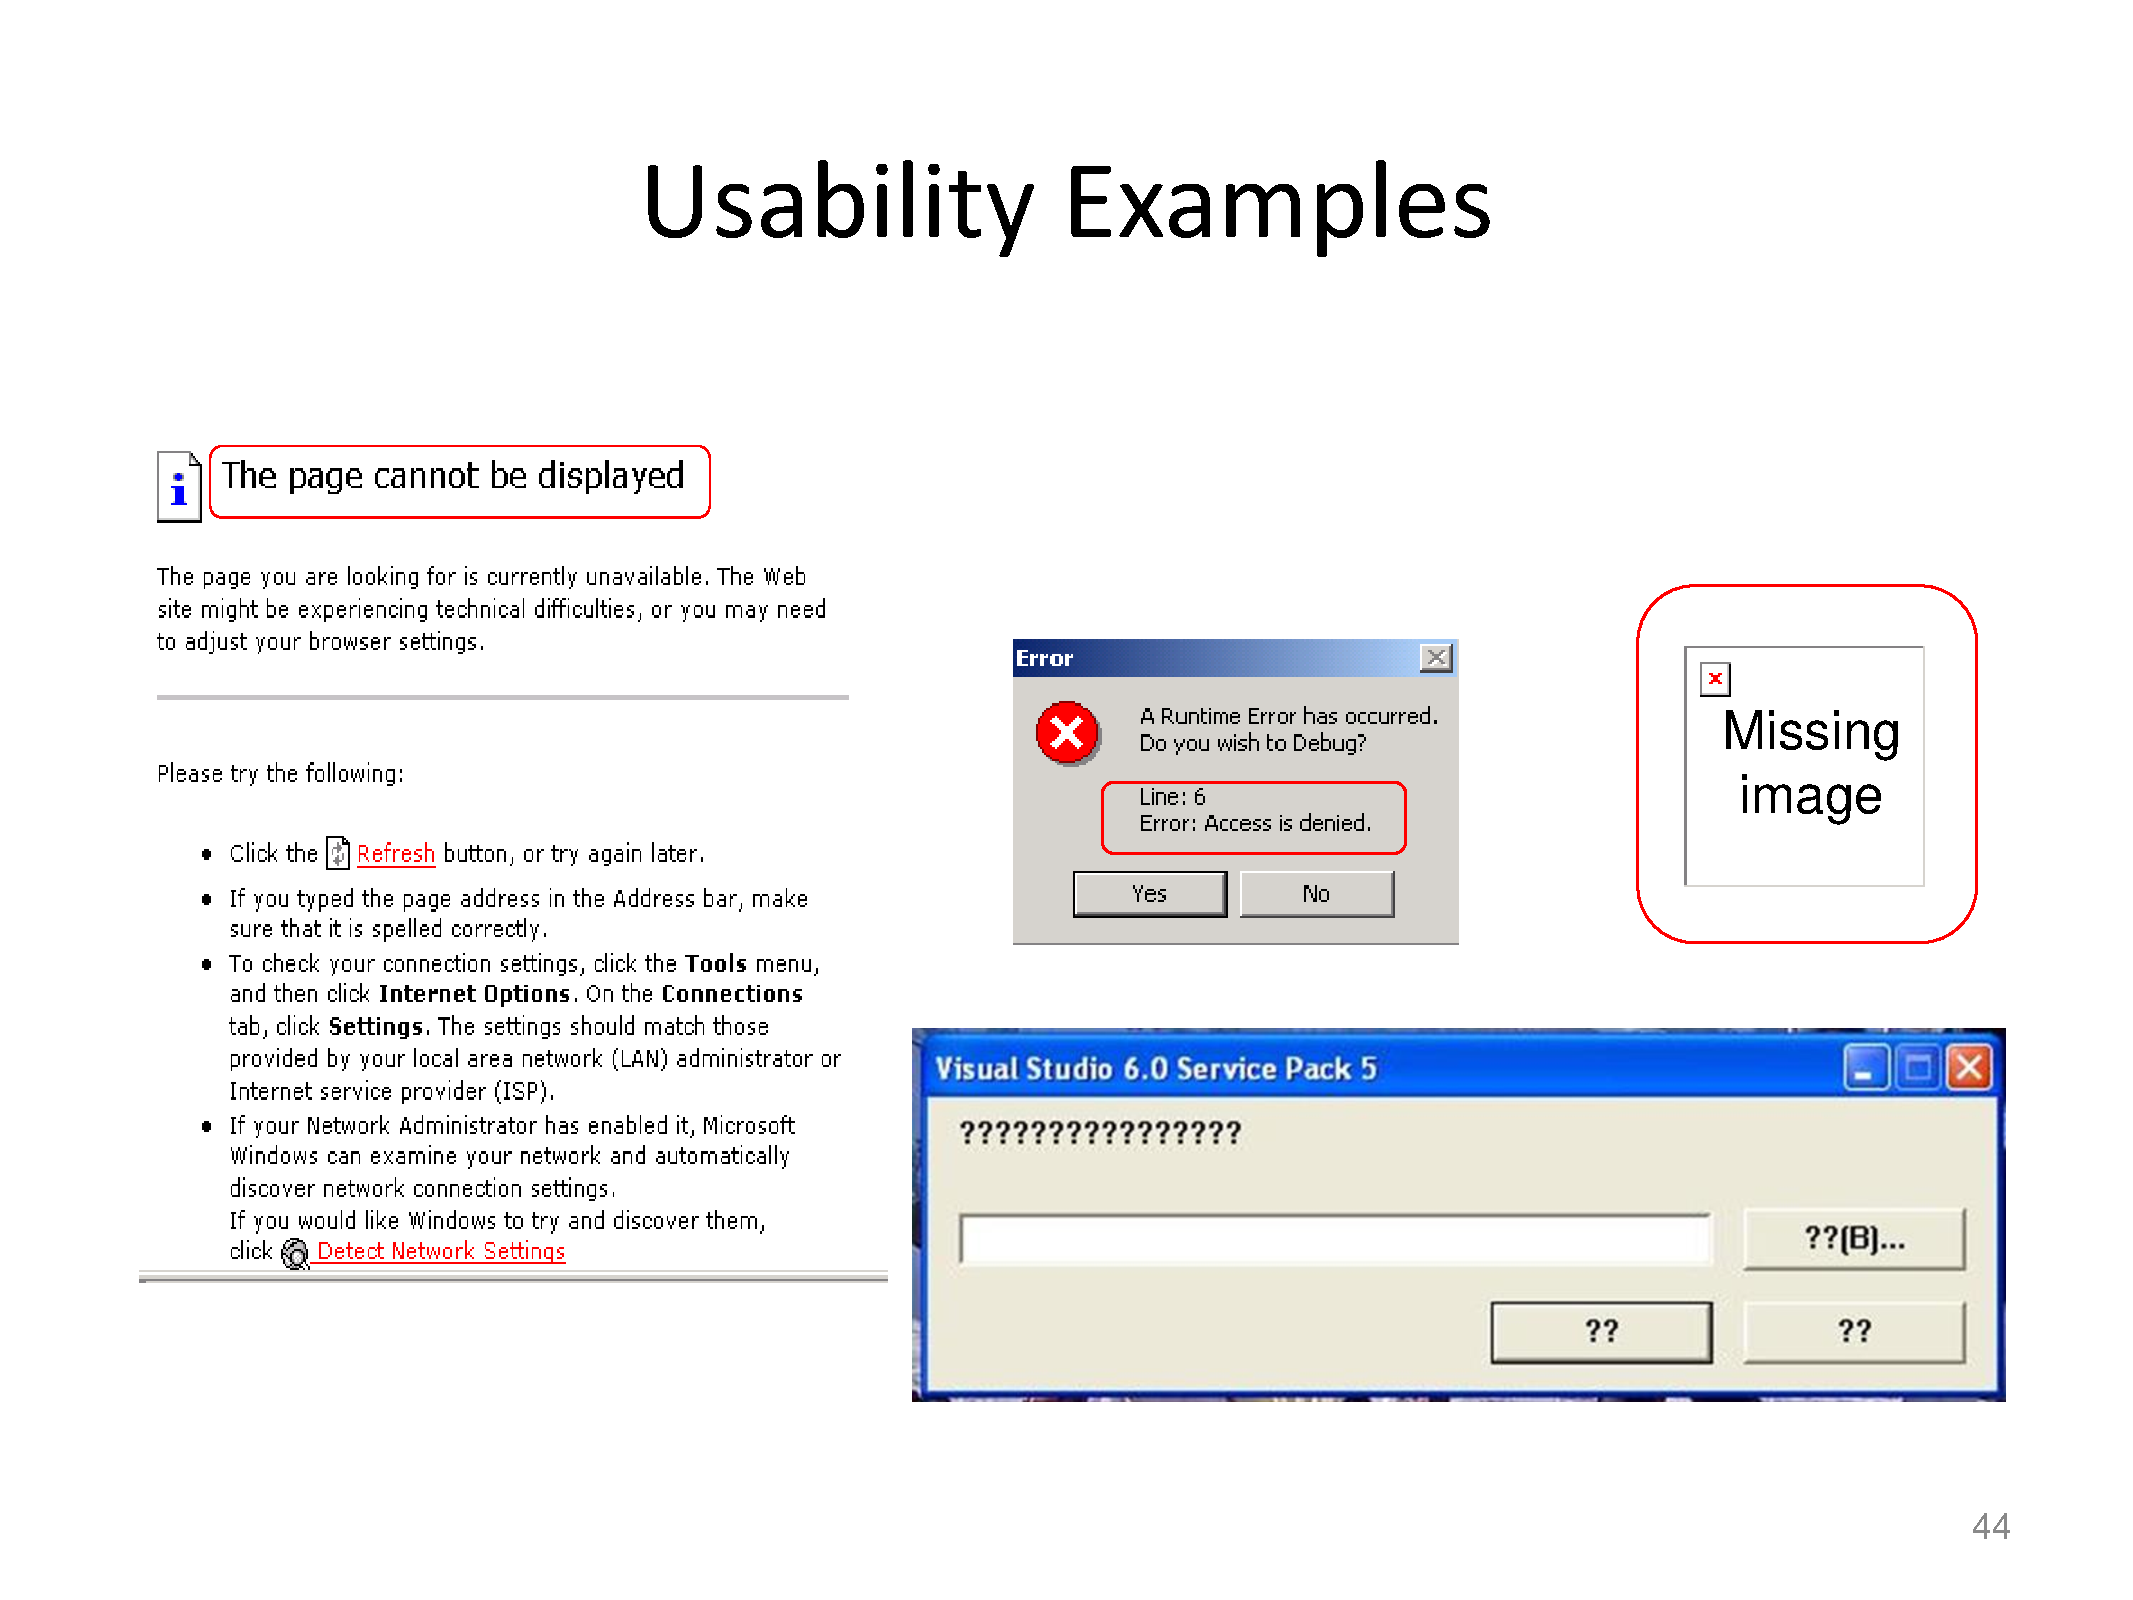
\includegraphics[width=\linewidth]{340.pdf}\\
        \textbf{Compatibility Testing}: ensures product functionality \& reliability on supported browsers \& platforms that exist on customer computer\\
        \vfill\null\columnbreak\noindent\underline{\textbf{Week 8}}\\
        \textbf{Test management}: manage test plans \& cases, track requirements \& defects, execute tests, measure progress\\
        \textbf{Test Report Contents}:\\
        \textit{Test objective}: identifying objectives of testing, should be planned so all requirements individually tested, state exit criteria\\
        \textit{Test environment}: description of test tools, required packages, hardware \& software environment\\
        \textit{Modules (features) under test \& test cases}: software modules to be tested \& corresponding test cases, expected \& actual test results\\
        \textit{Testing schedule}: overall test schedule \& resource allocation\\
        \textit{Test Summary}: summary \& analysis of test results, test coverage report\\
        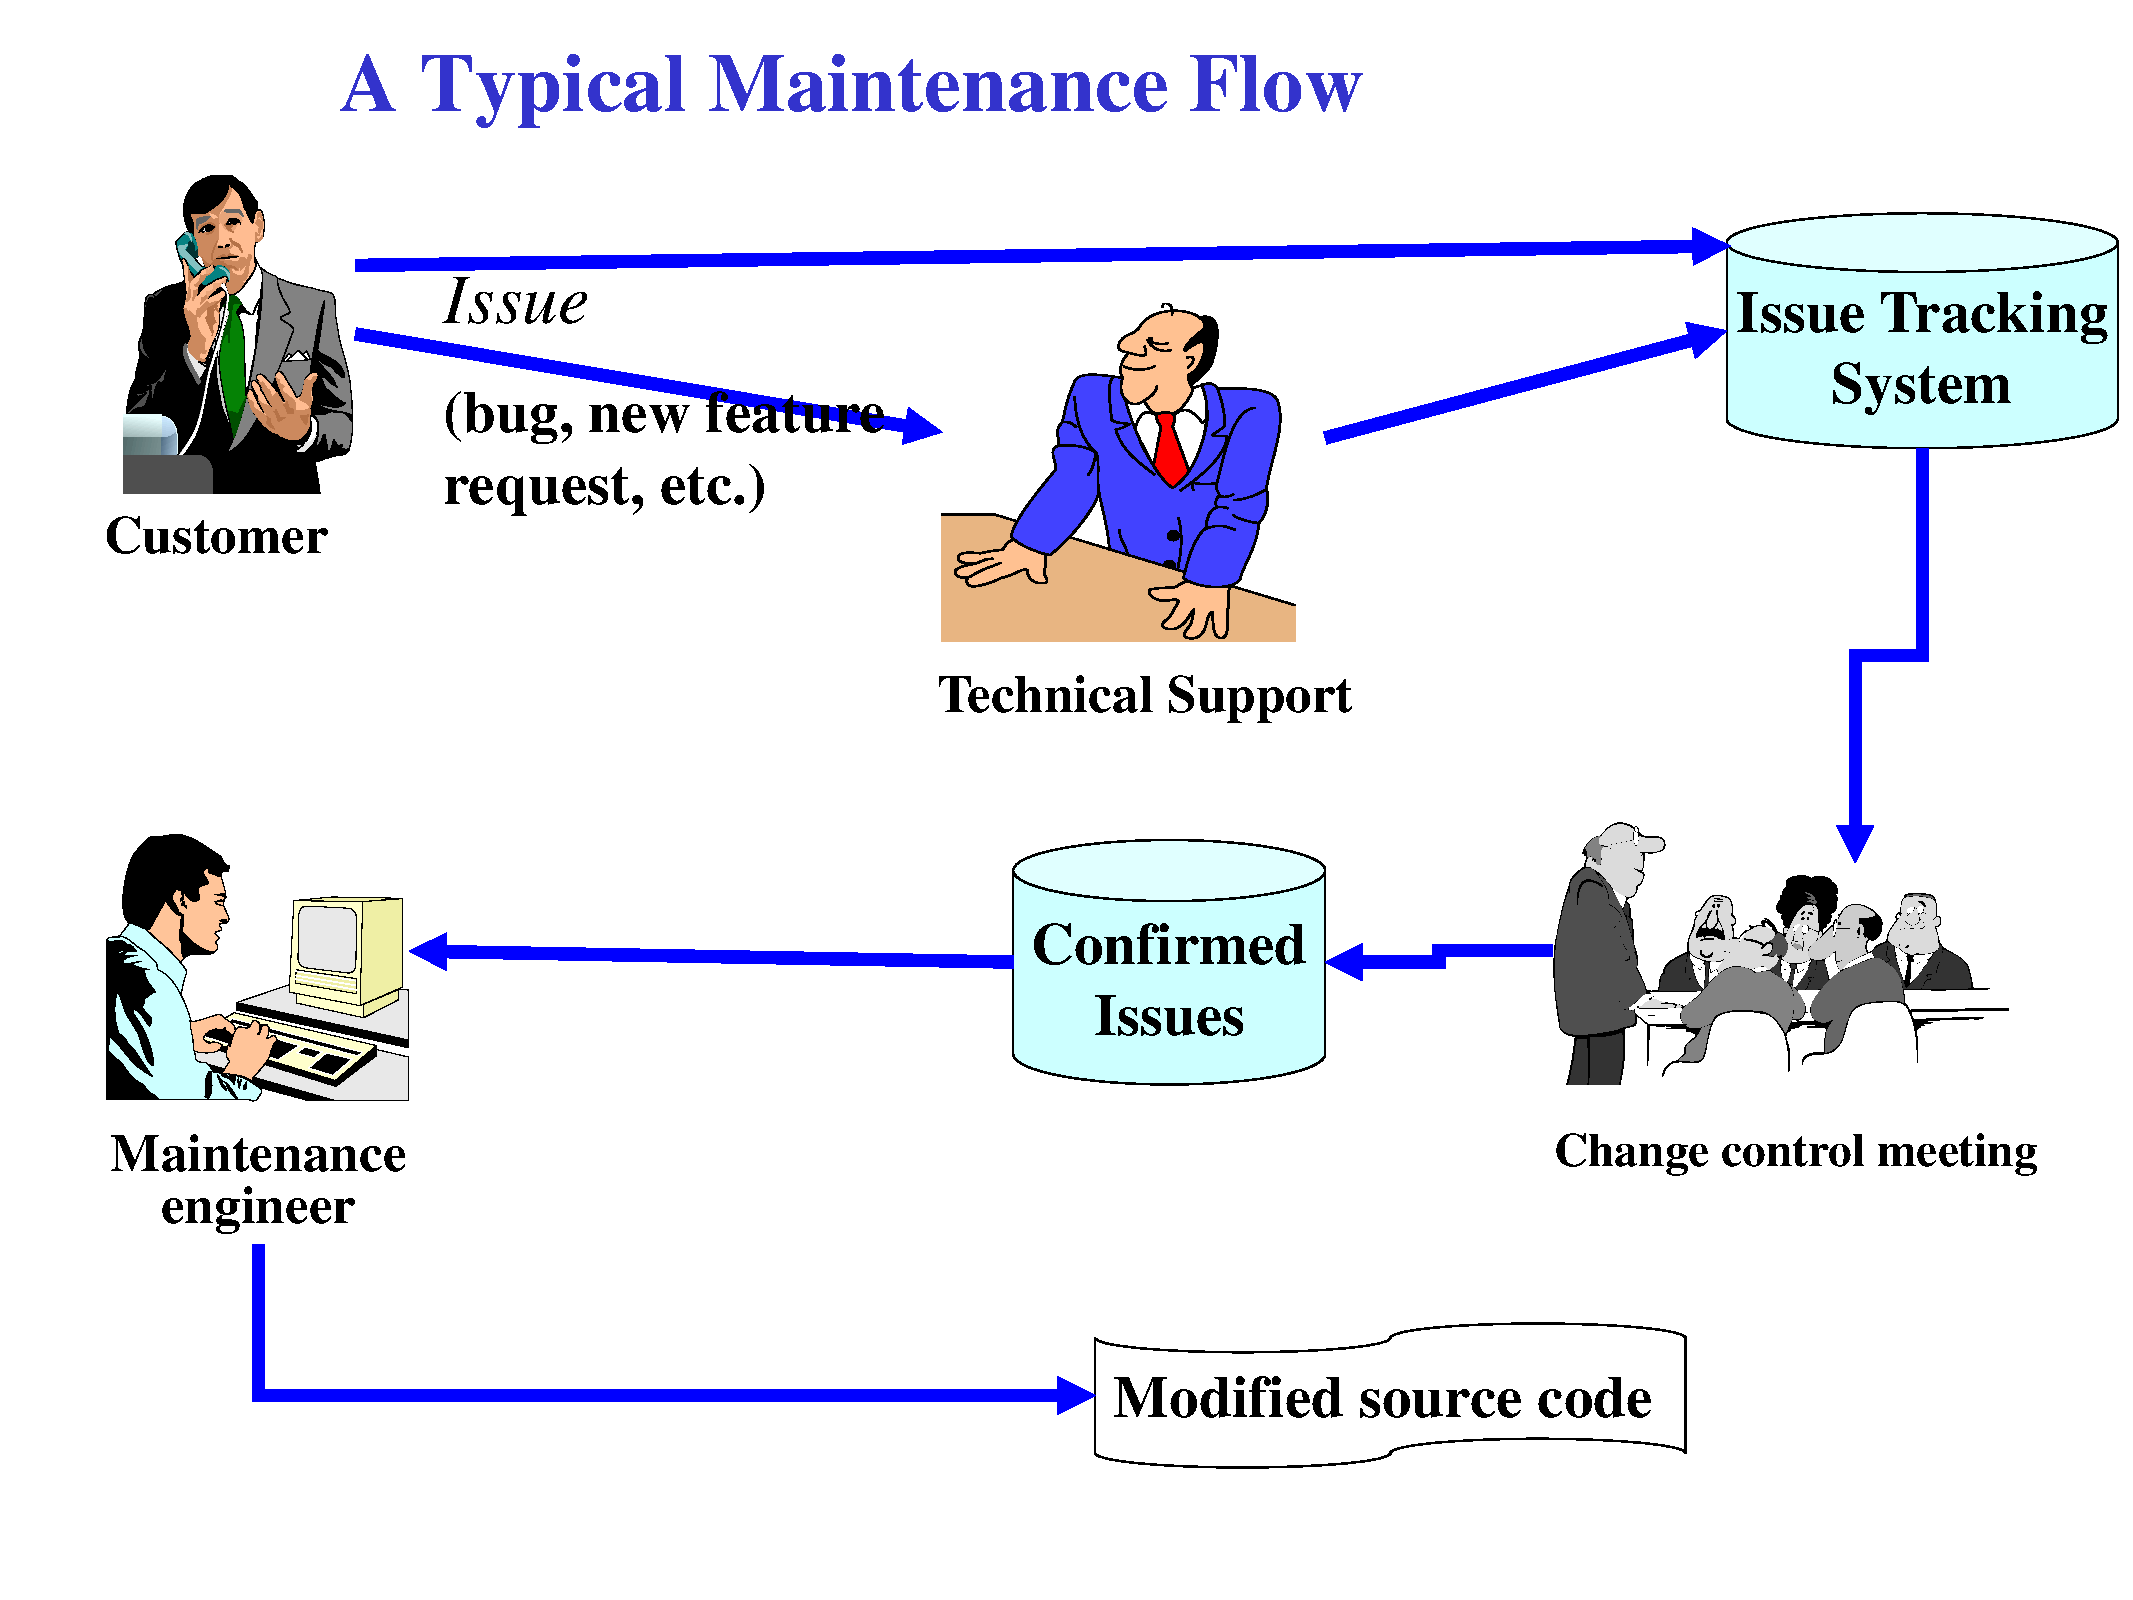
\includegraphics[width=\linewidth]{355.pdf}\\
        \textbf{Issue Tracking System}: software tool designed to help devs keep track of reported software issues (including bugs \& new feature requests), extremely valuable in software development, used extensively by companies developing software products\\
        \textbf{Issue Tracking System Uses}: track issues/bugs, communicate with teammates, submit \& review patches, manage quality assurance\\
        \textbf{Bug Data}:\\
        \textit{Description}: summary, product/module it belongs to, detailed descriptions\\
        \textit{Role}: reporter/submitter, assignee, QA contact\\
        \textit{Status}: current status, resolution, priority, severity\\
        \textit{Time}: open date, changed date, closed date, \ldots\\
        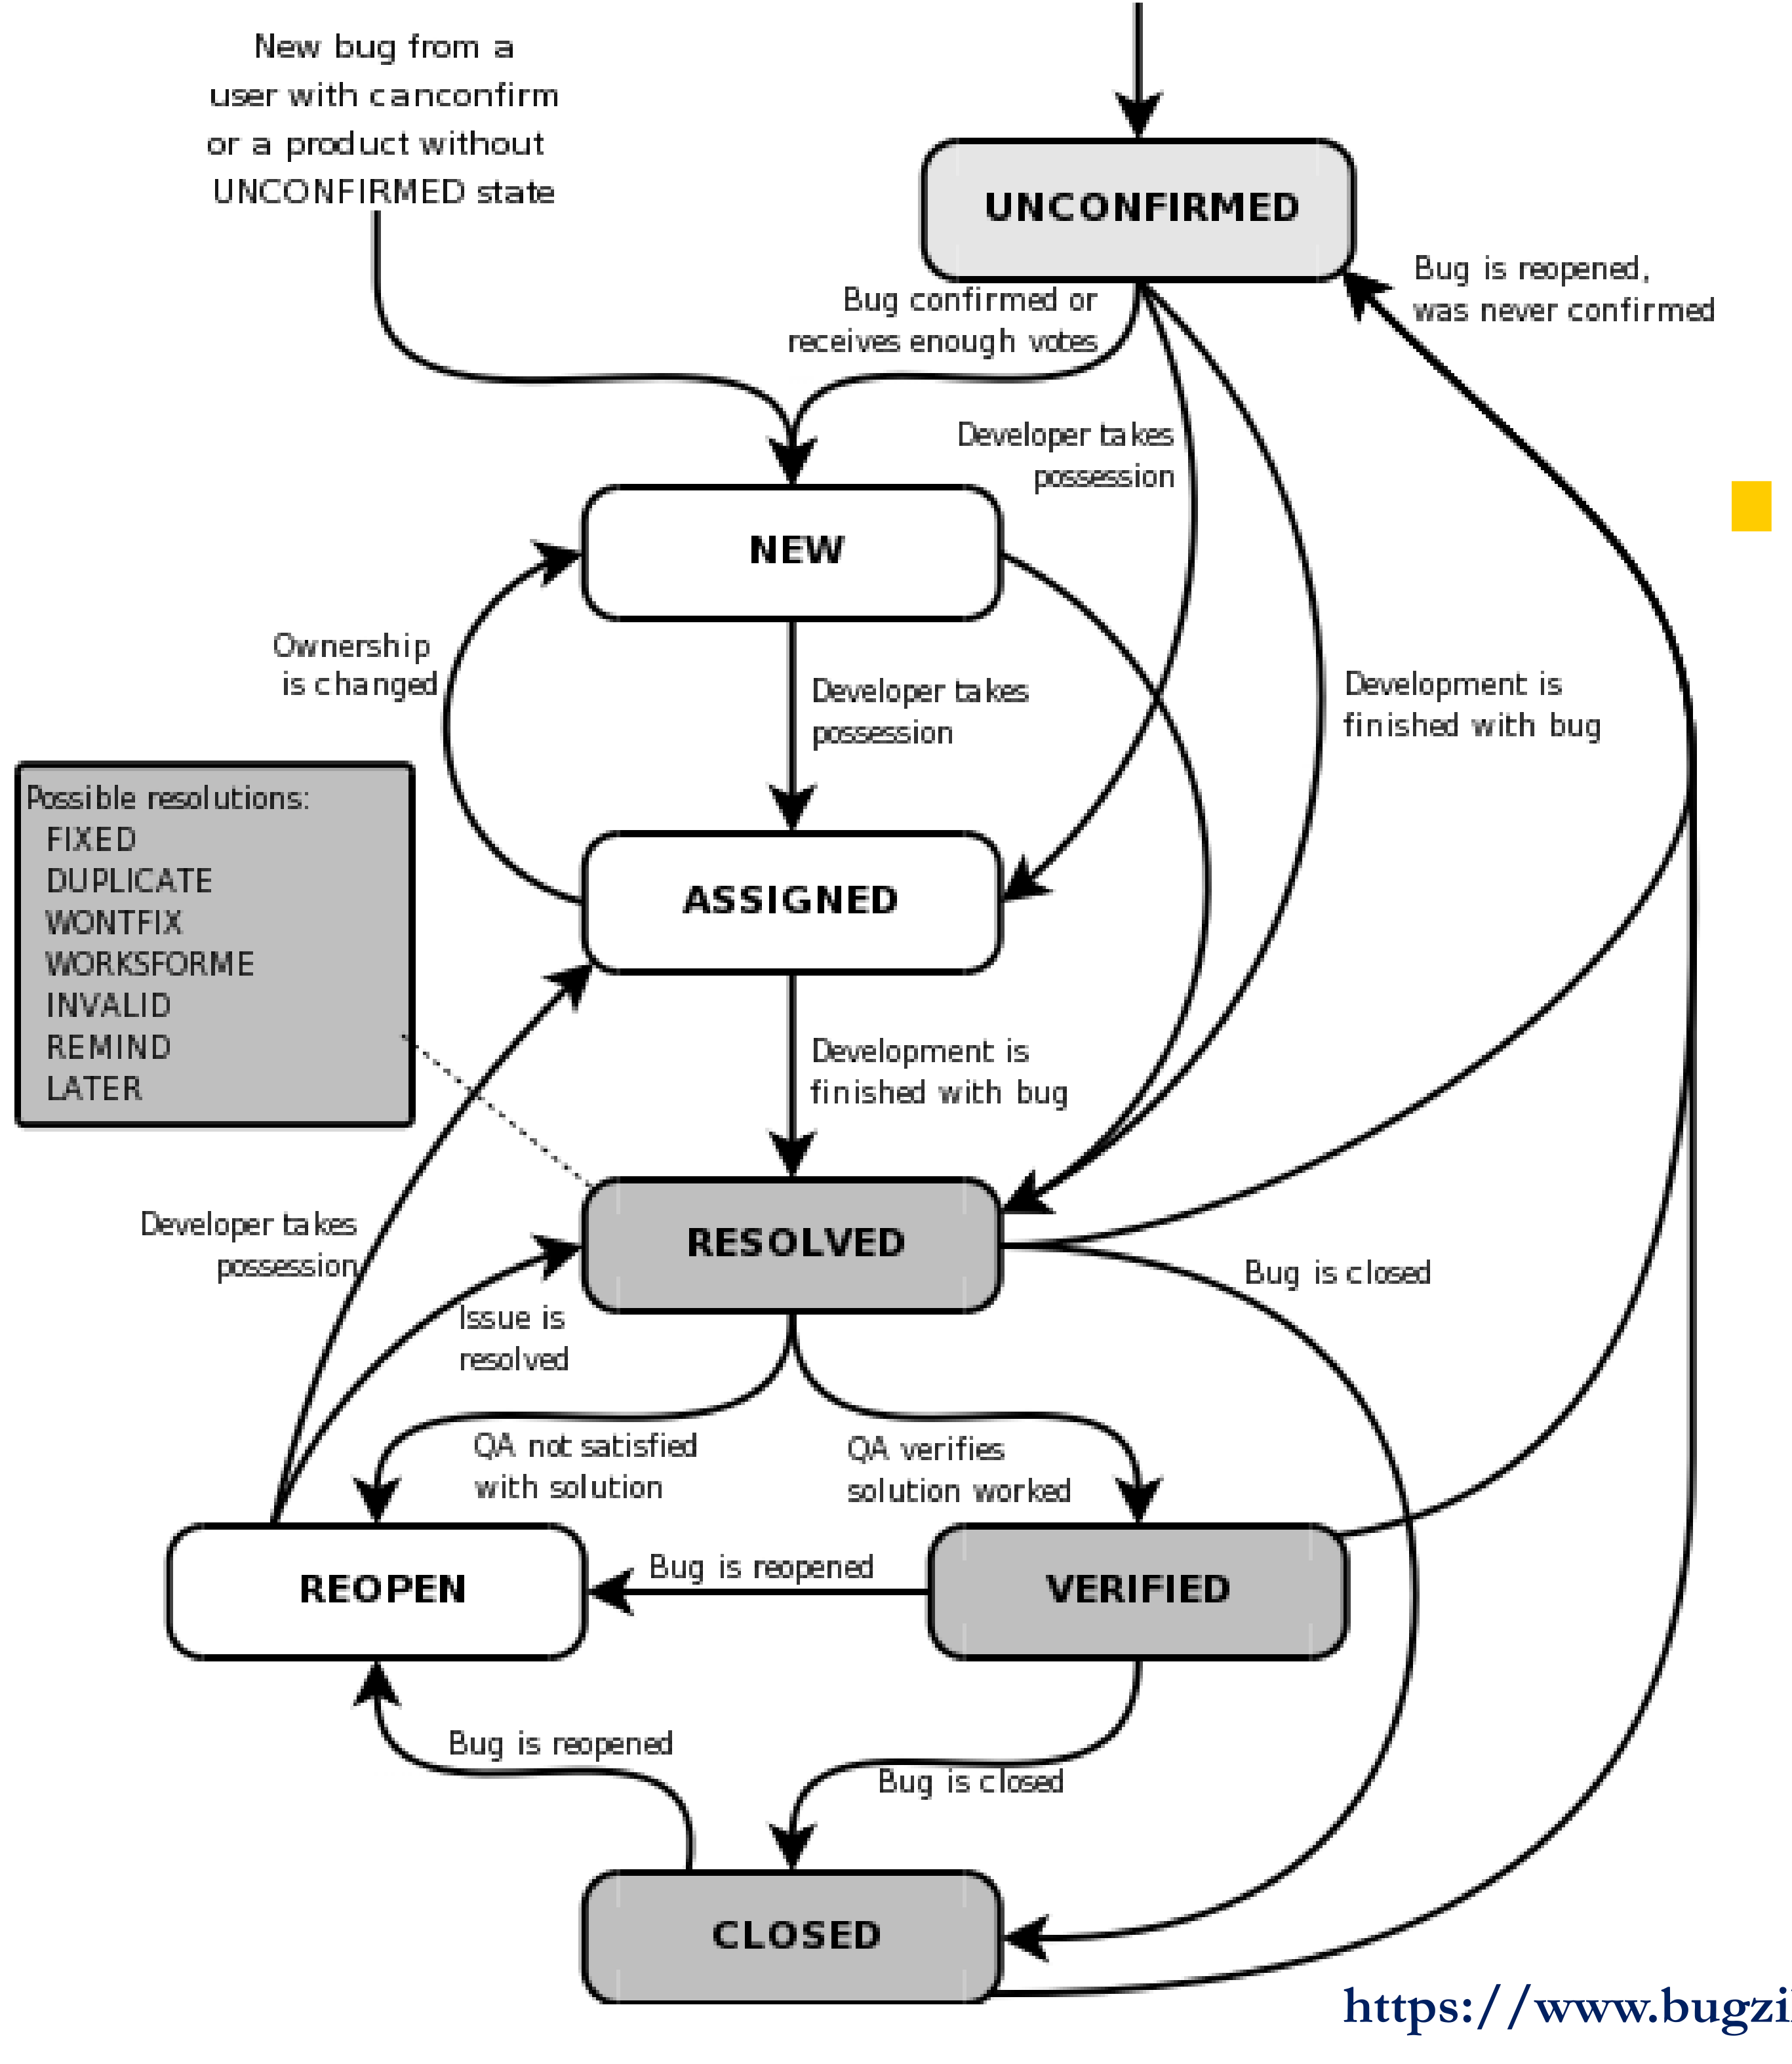
\includegraphics[width=\linewidth]{359.png}\\
        \textbf{Issue Tracking System Design}: database, business logic, client\\
        \textbf{Useful bug reports}: ones that get bugs fixed, reproducible, specific\\
        \textbf{Regression Testing}: run old test cases on new version, establishing policy for regular regression testing is key for achieving successful,reliable \& predictable software development projects\\
        \textbf{Regression Test Selection}: speed up regression testing by only rerunning tests affected by code changes\\
        \textbf{Regression Test Prioritisation}: rank all test cases (to discover bugs sooner or achieve higher coverage sooner), run test cases according to ranked sequence, stop when all resources used up\\
        \textbf{Reliability}: probability that system/capability of system functions without failure for specified time in specified environment, ex: reliability of 0.92 for 8 hours means when executed for that long would operate without failure for 92 out of 100 periods\\
        \textbf{Single failure specification}: what is probability of failure of a system/component\\
        \textbf{Multiple failure specification}: if system/component fails at time $t_1,t_2, \ldots, t_{i-1}$m what is probability of failure at time $t_i$\\
        \textbf{Reliability formulas}: $R(t) = P(T > t), F(t) = P(T \leq t), t \geq 0$\\
        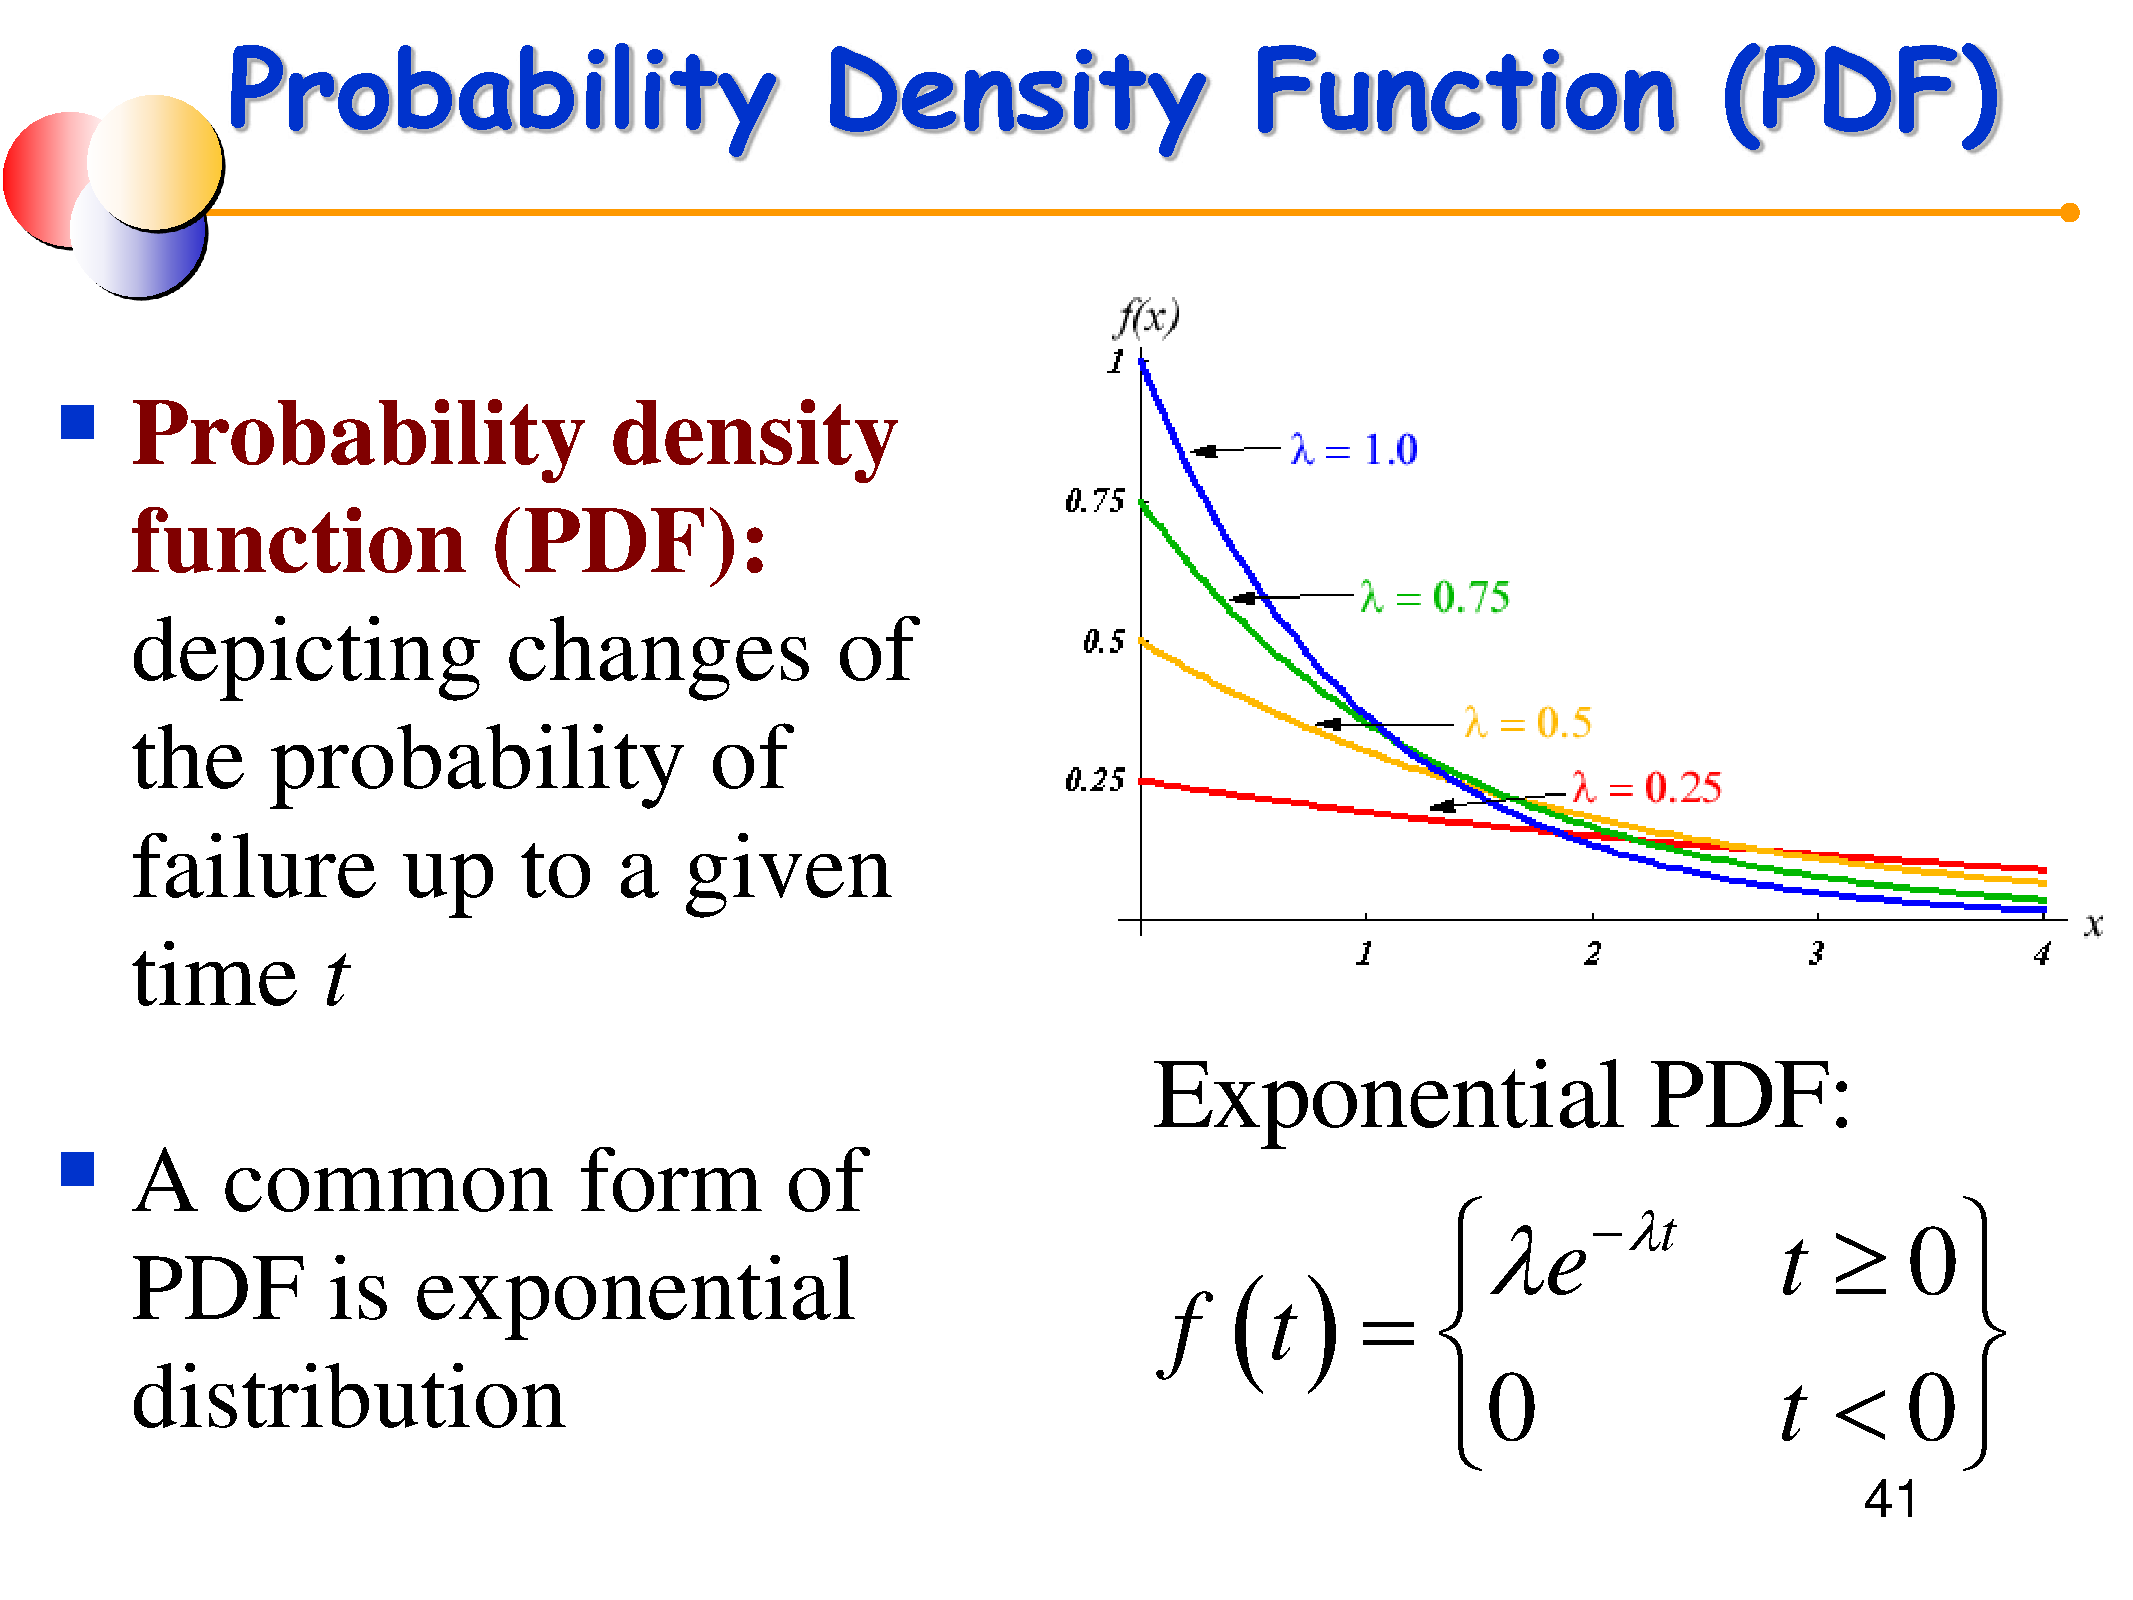
\includegraphics[width=\linewidth]{385.pdf}\\
        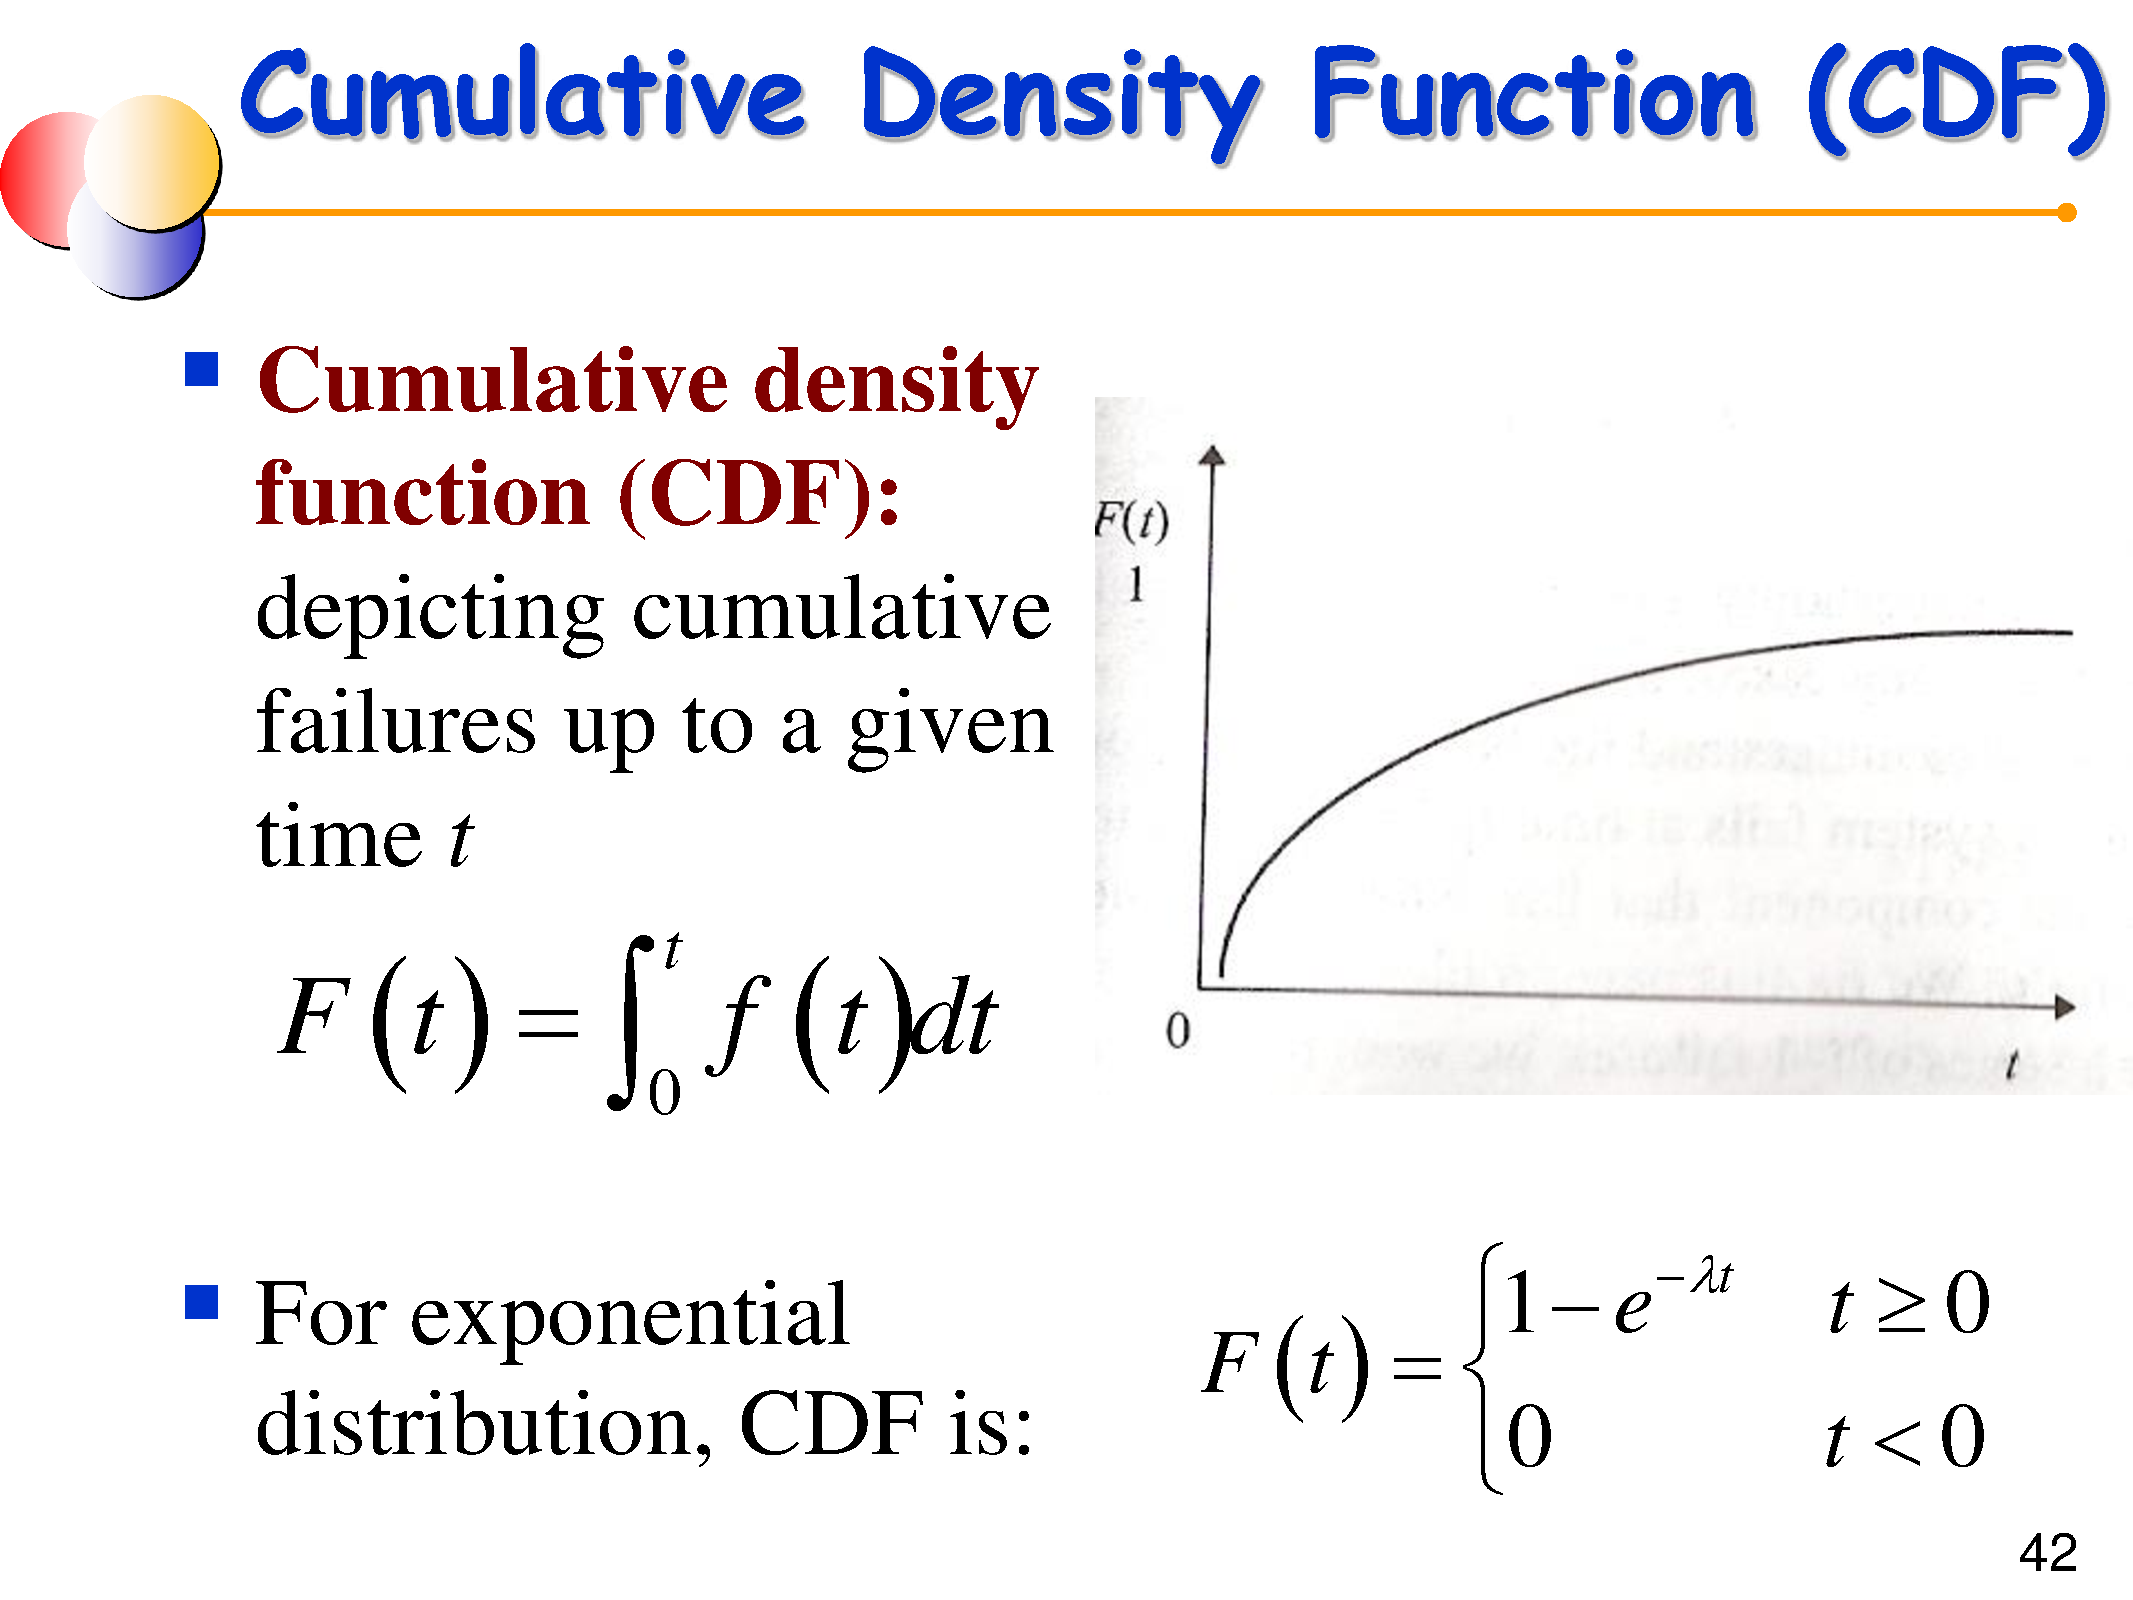
\includegraphics[width=\linewidth]{386.pdf}\\
        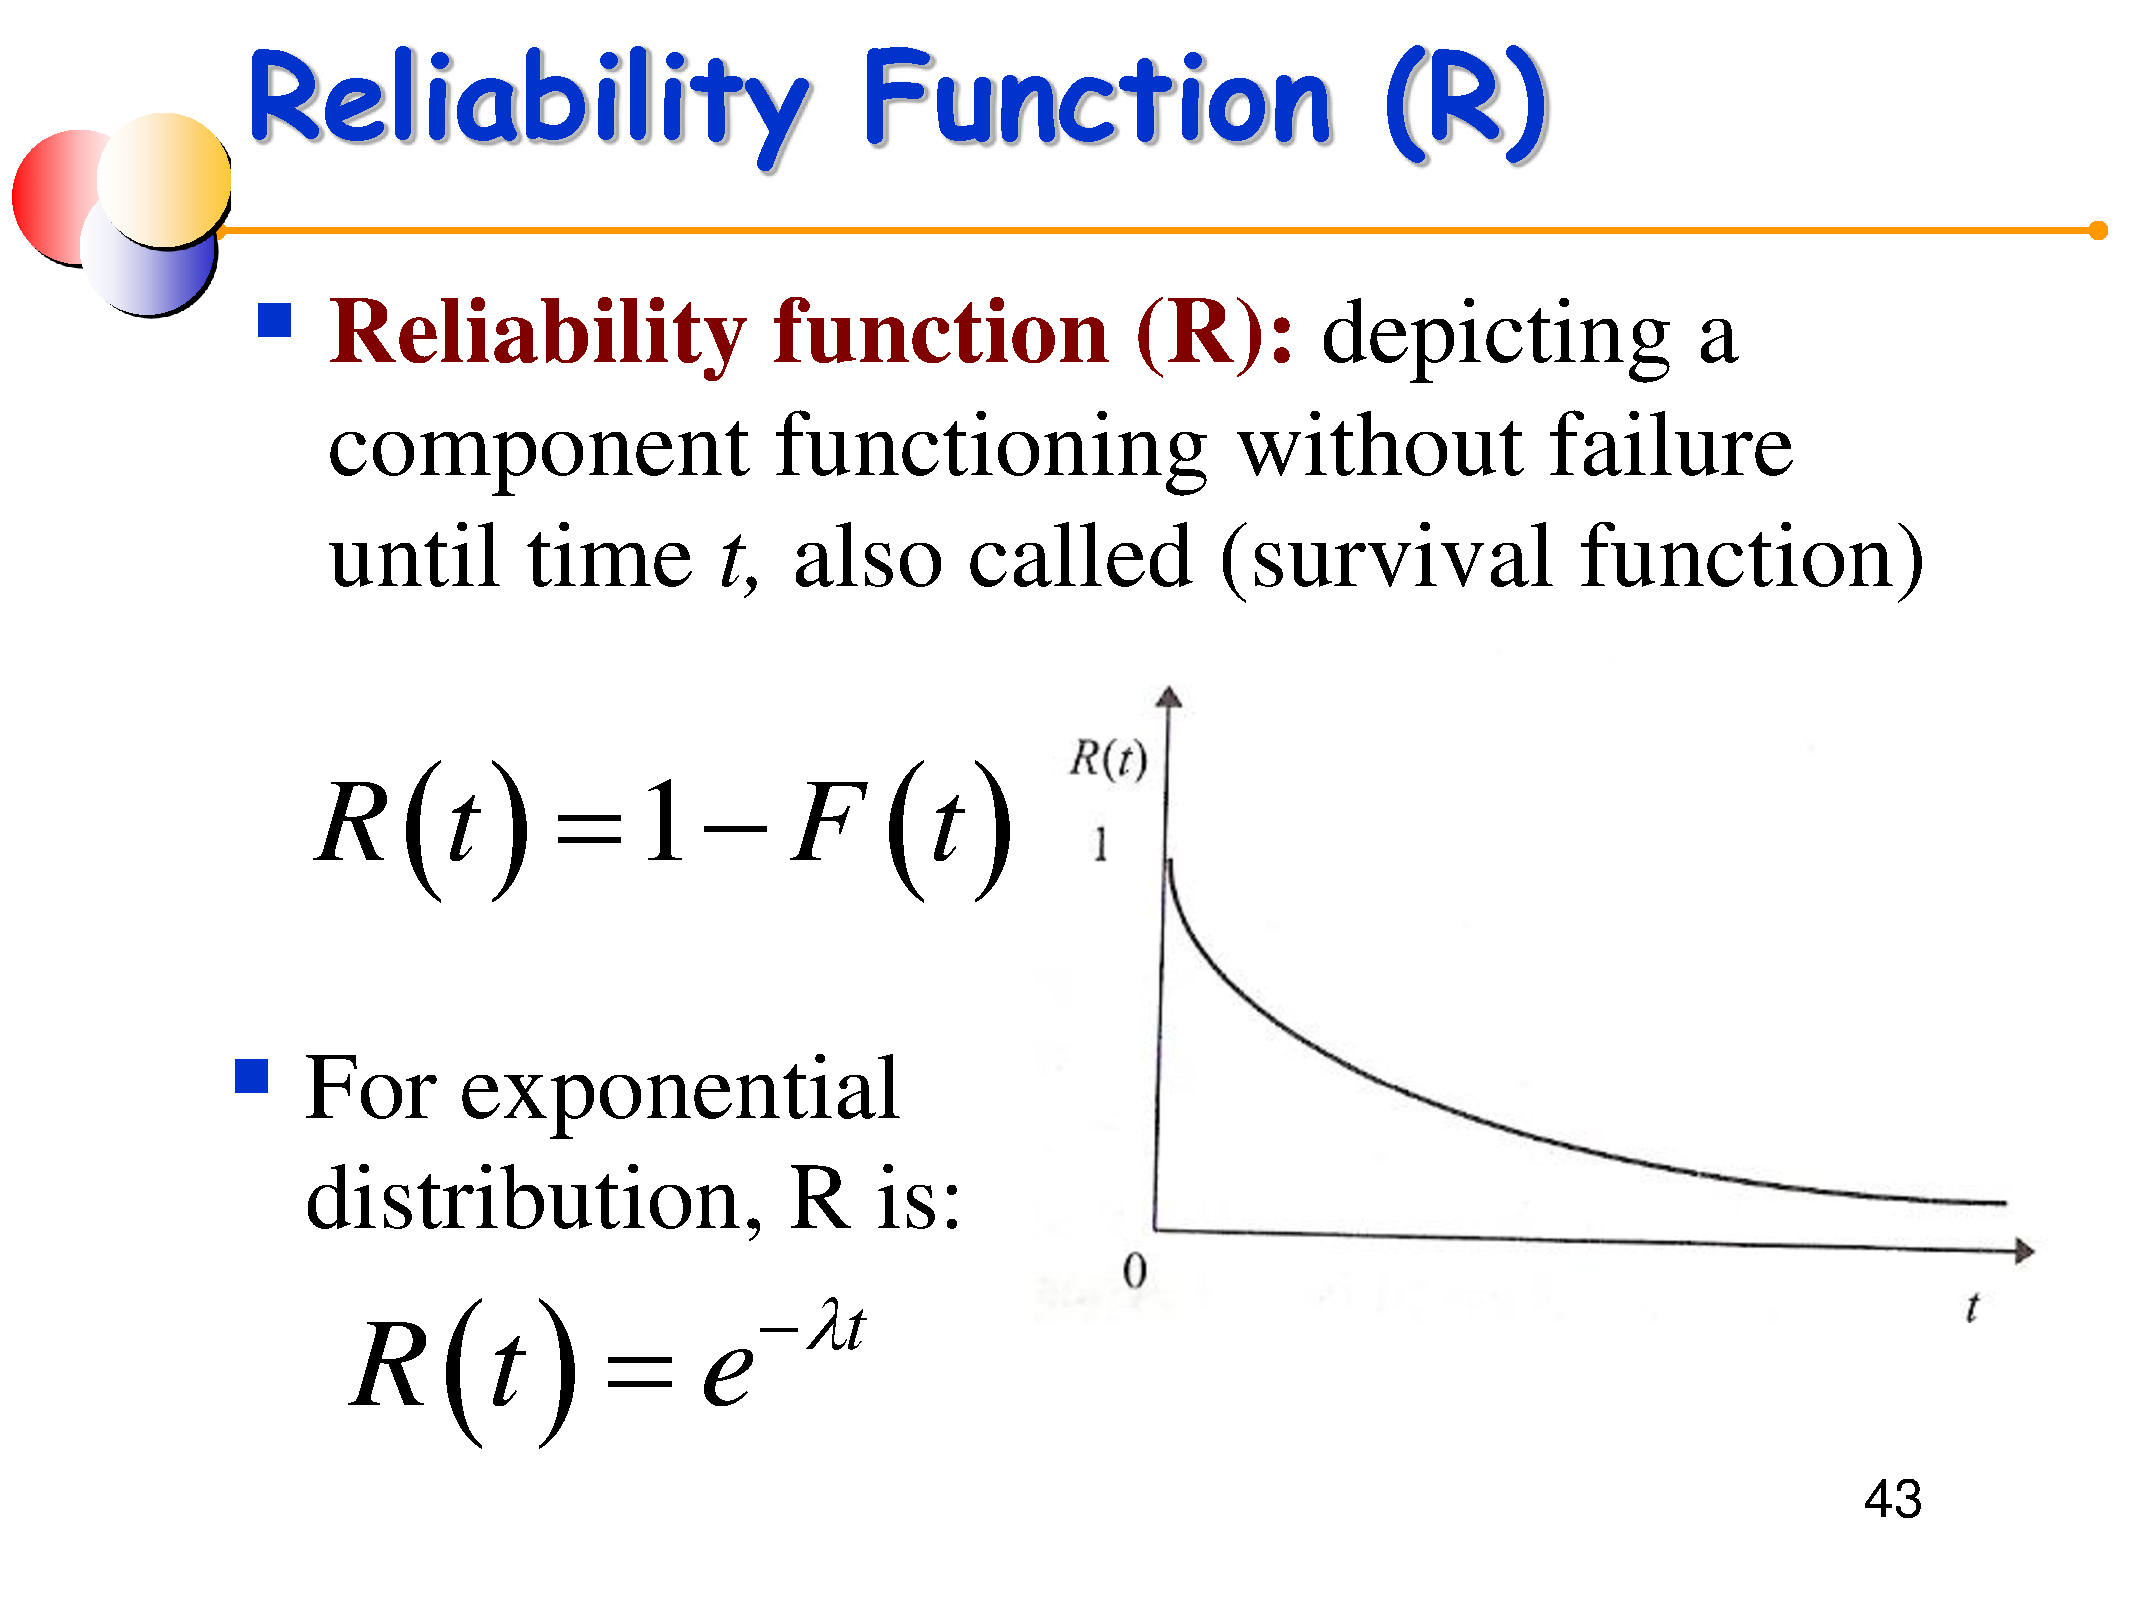
\includegraphics[width=\linewidth]{387.pdf}\\
        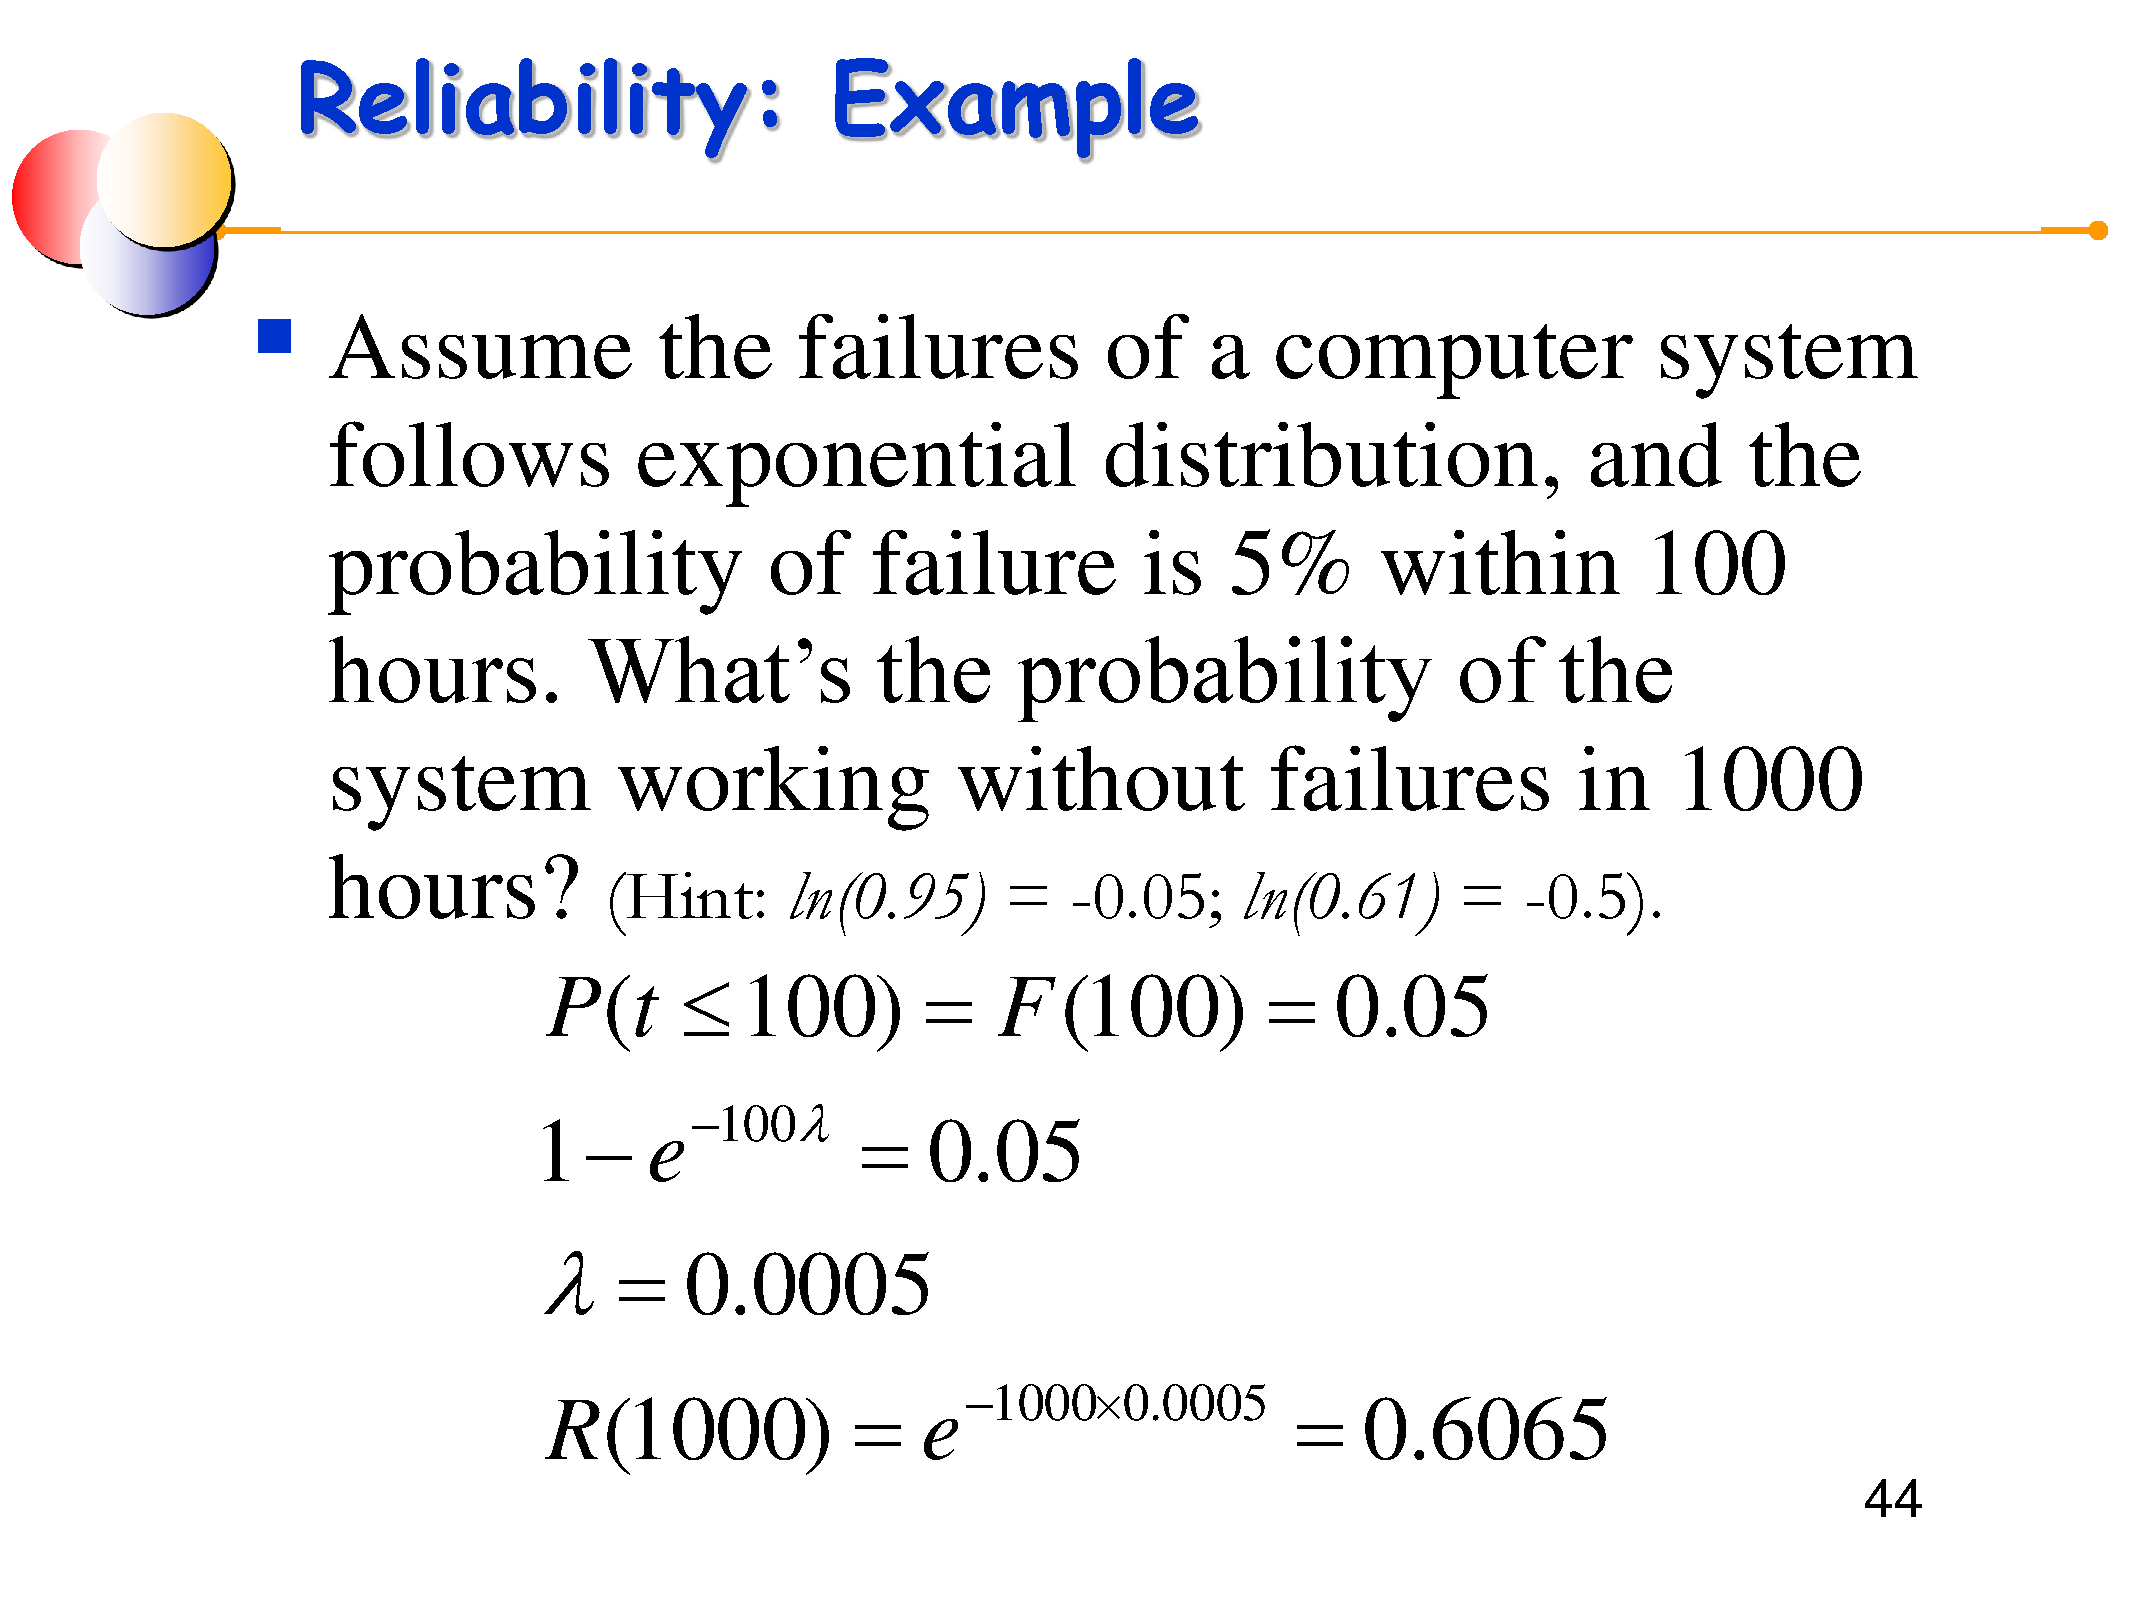
\includegraphics[width=\linewidth]{388.pdf}\\
        \textbf{Reliability Distributions}: exponential, Poisson, lognormal, normal, Pareto, Weibull\\
        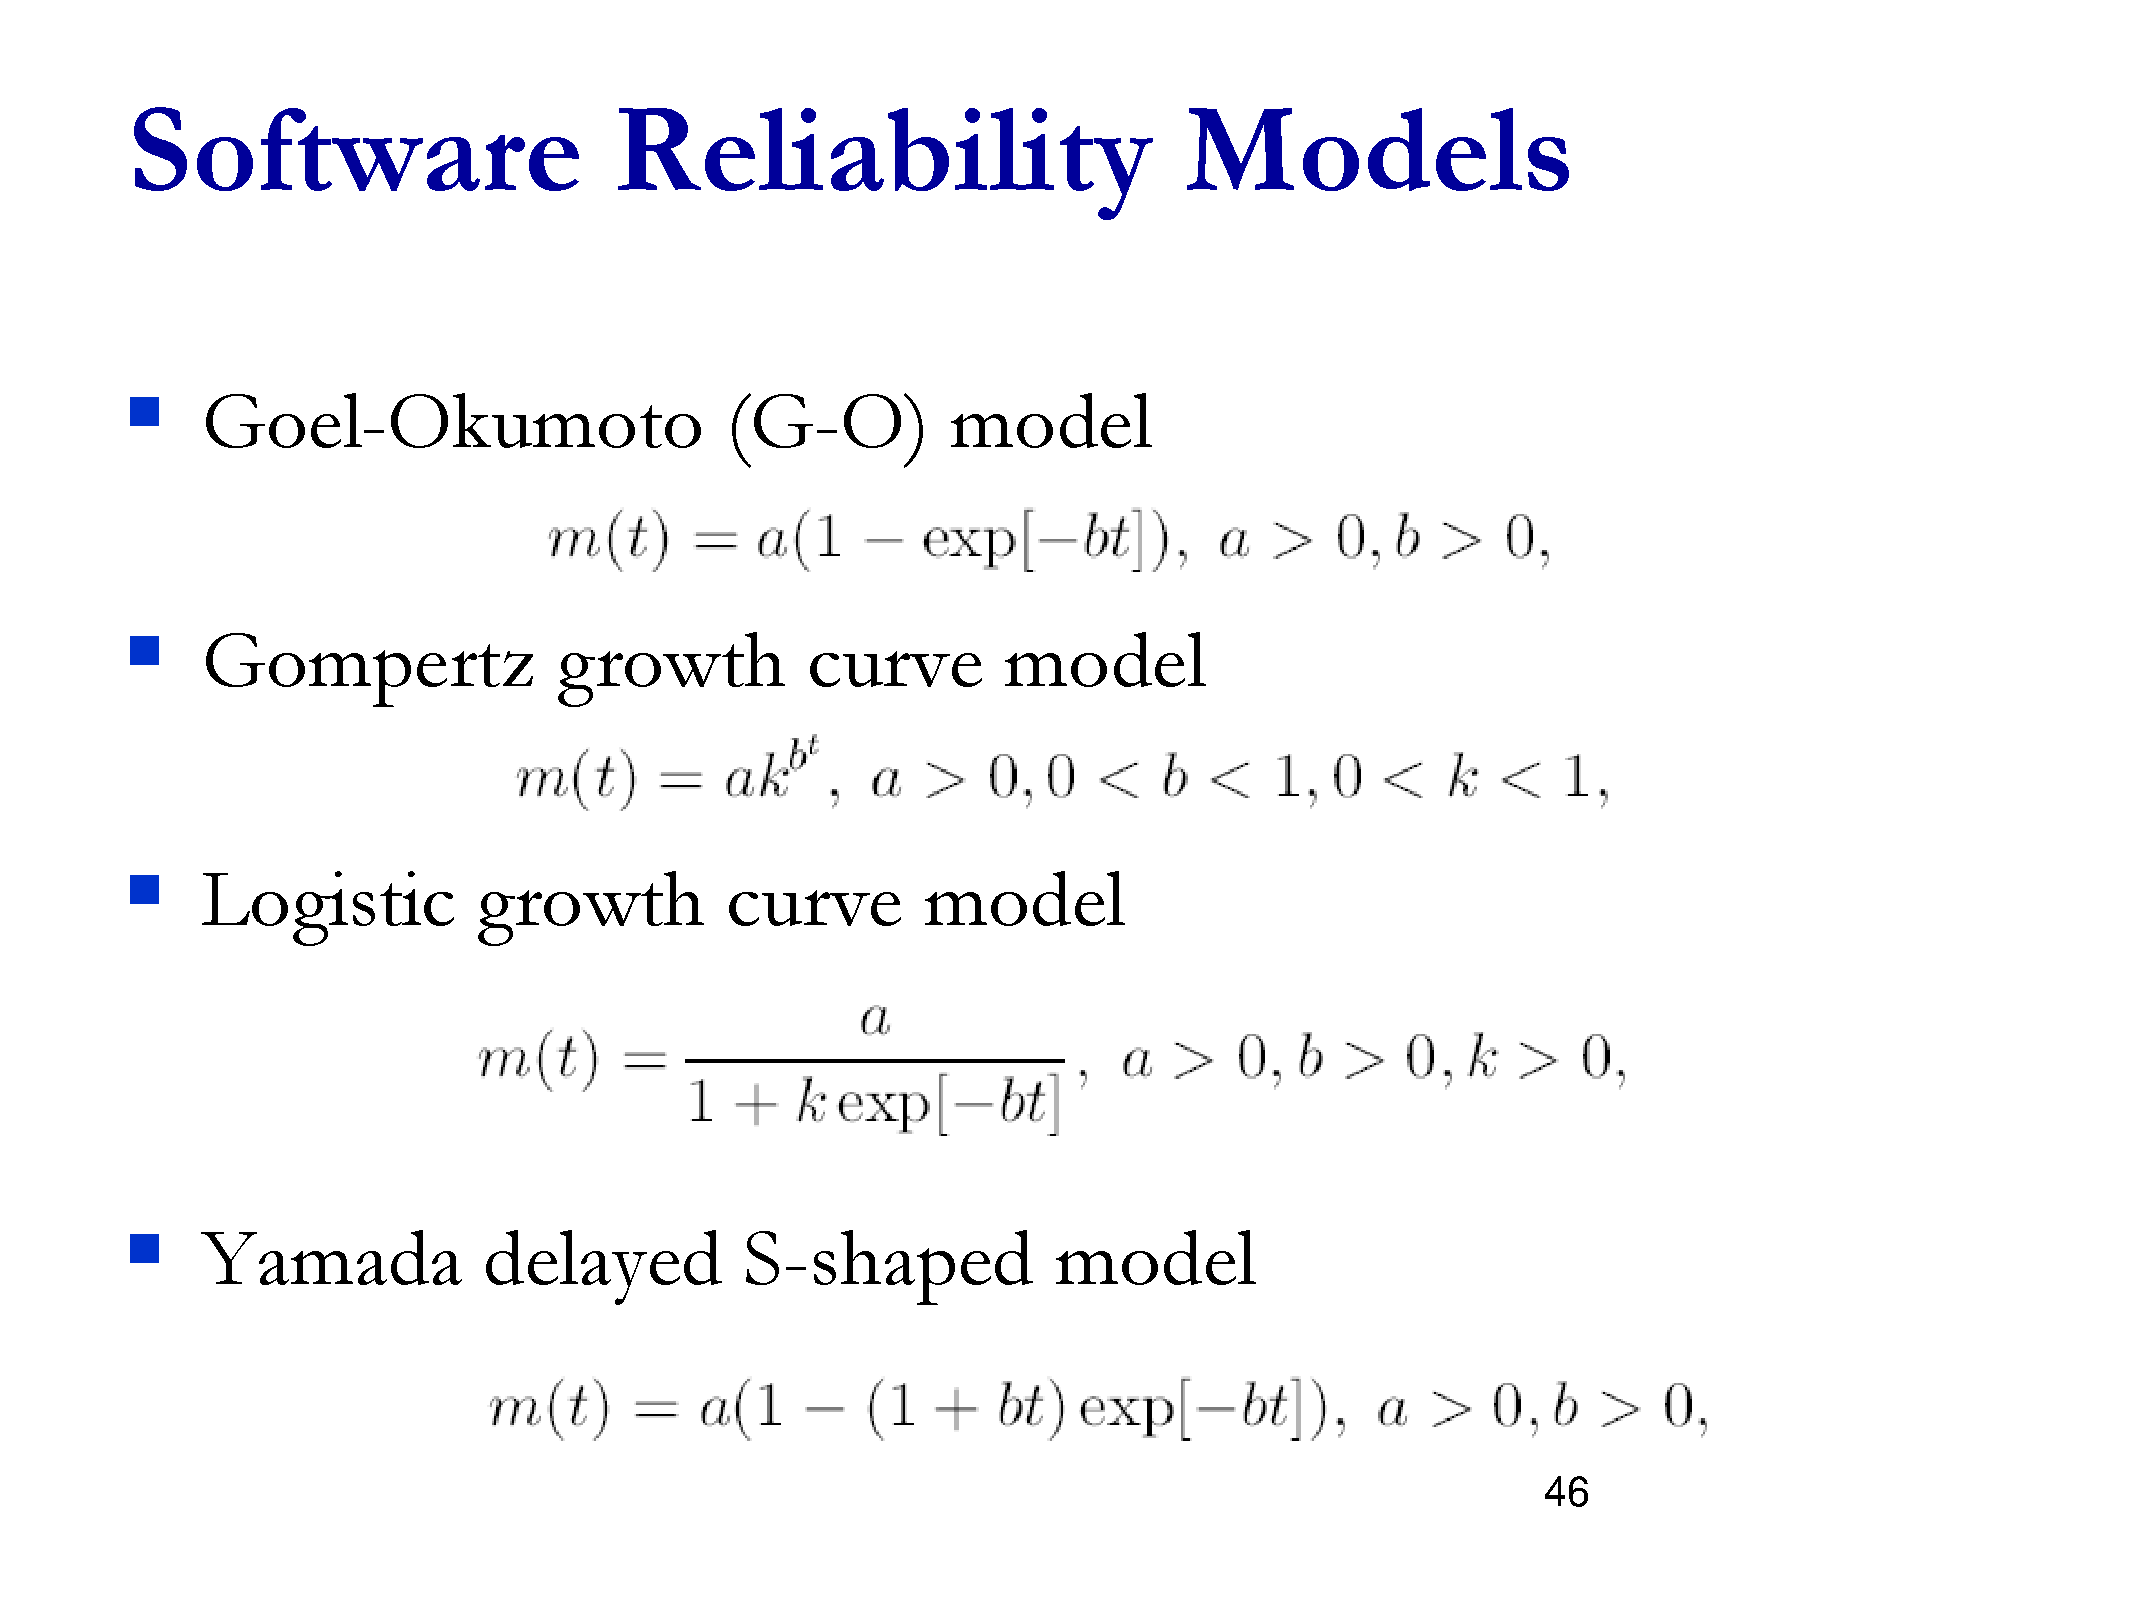
\includegraphics[width=\linewidth]{390.pdf}\\
        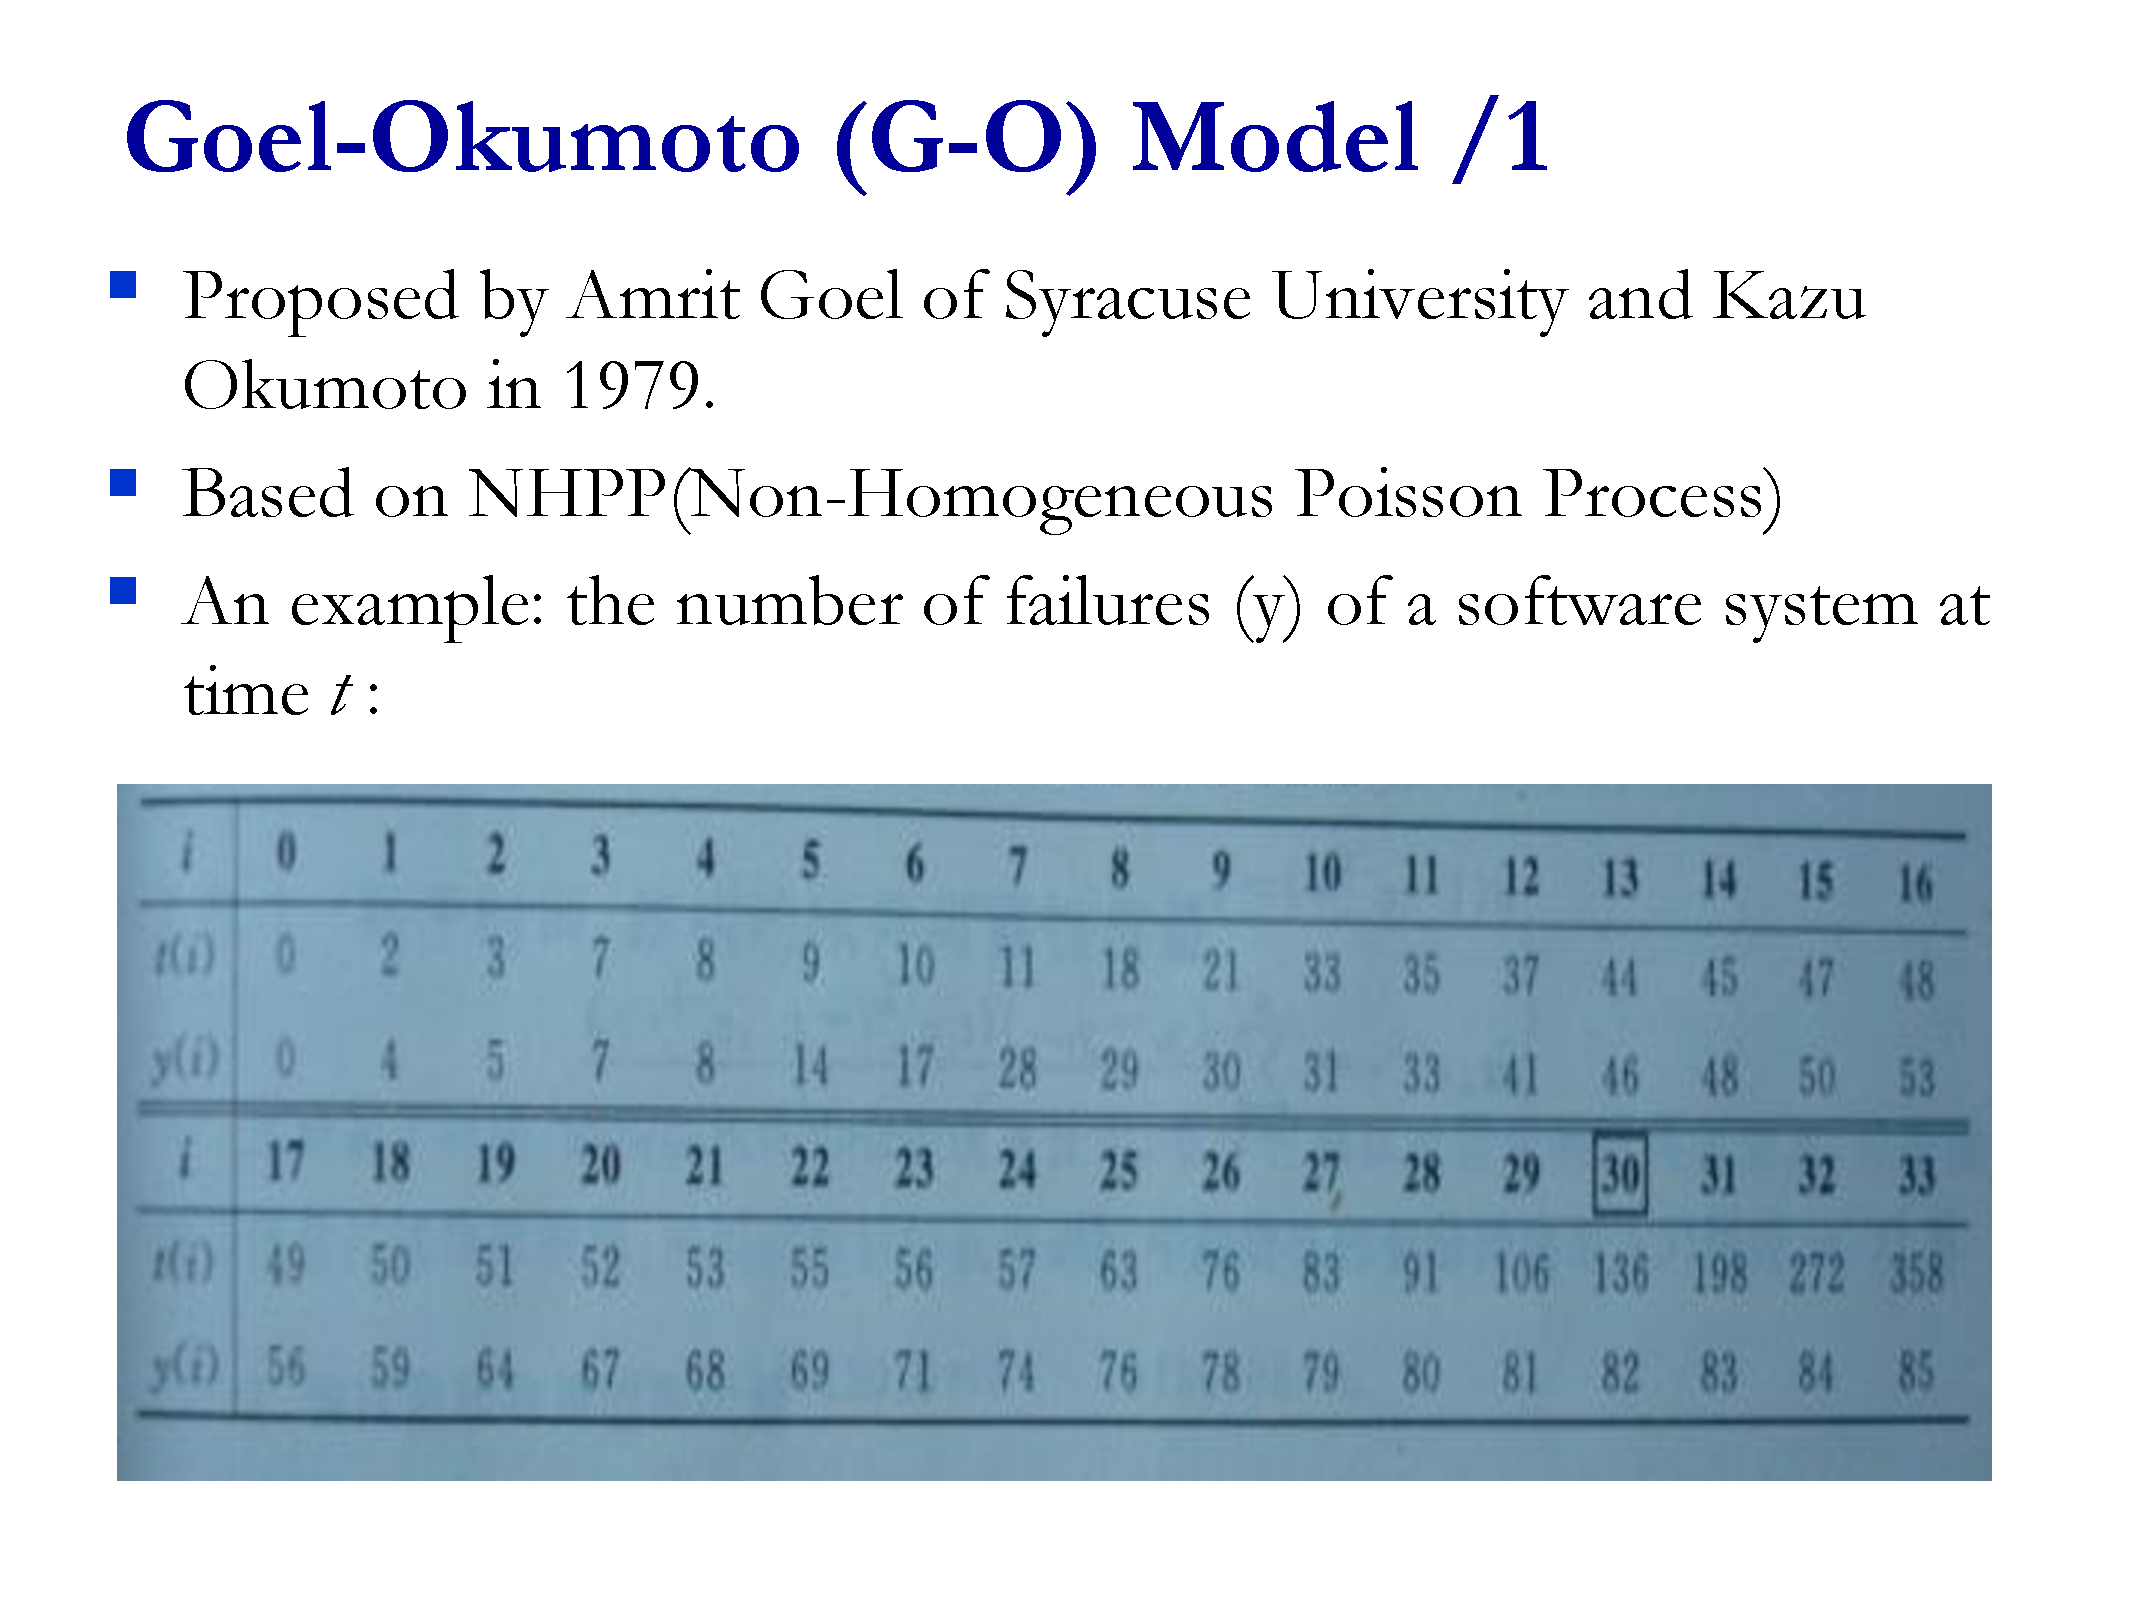
\includegraphics[width=\linewidth]{391.pdf}\\
        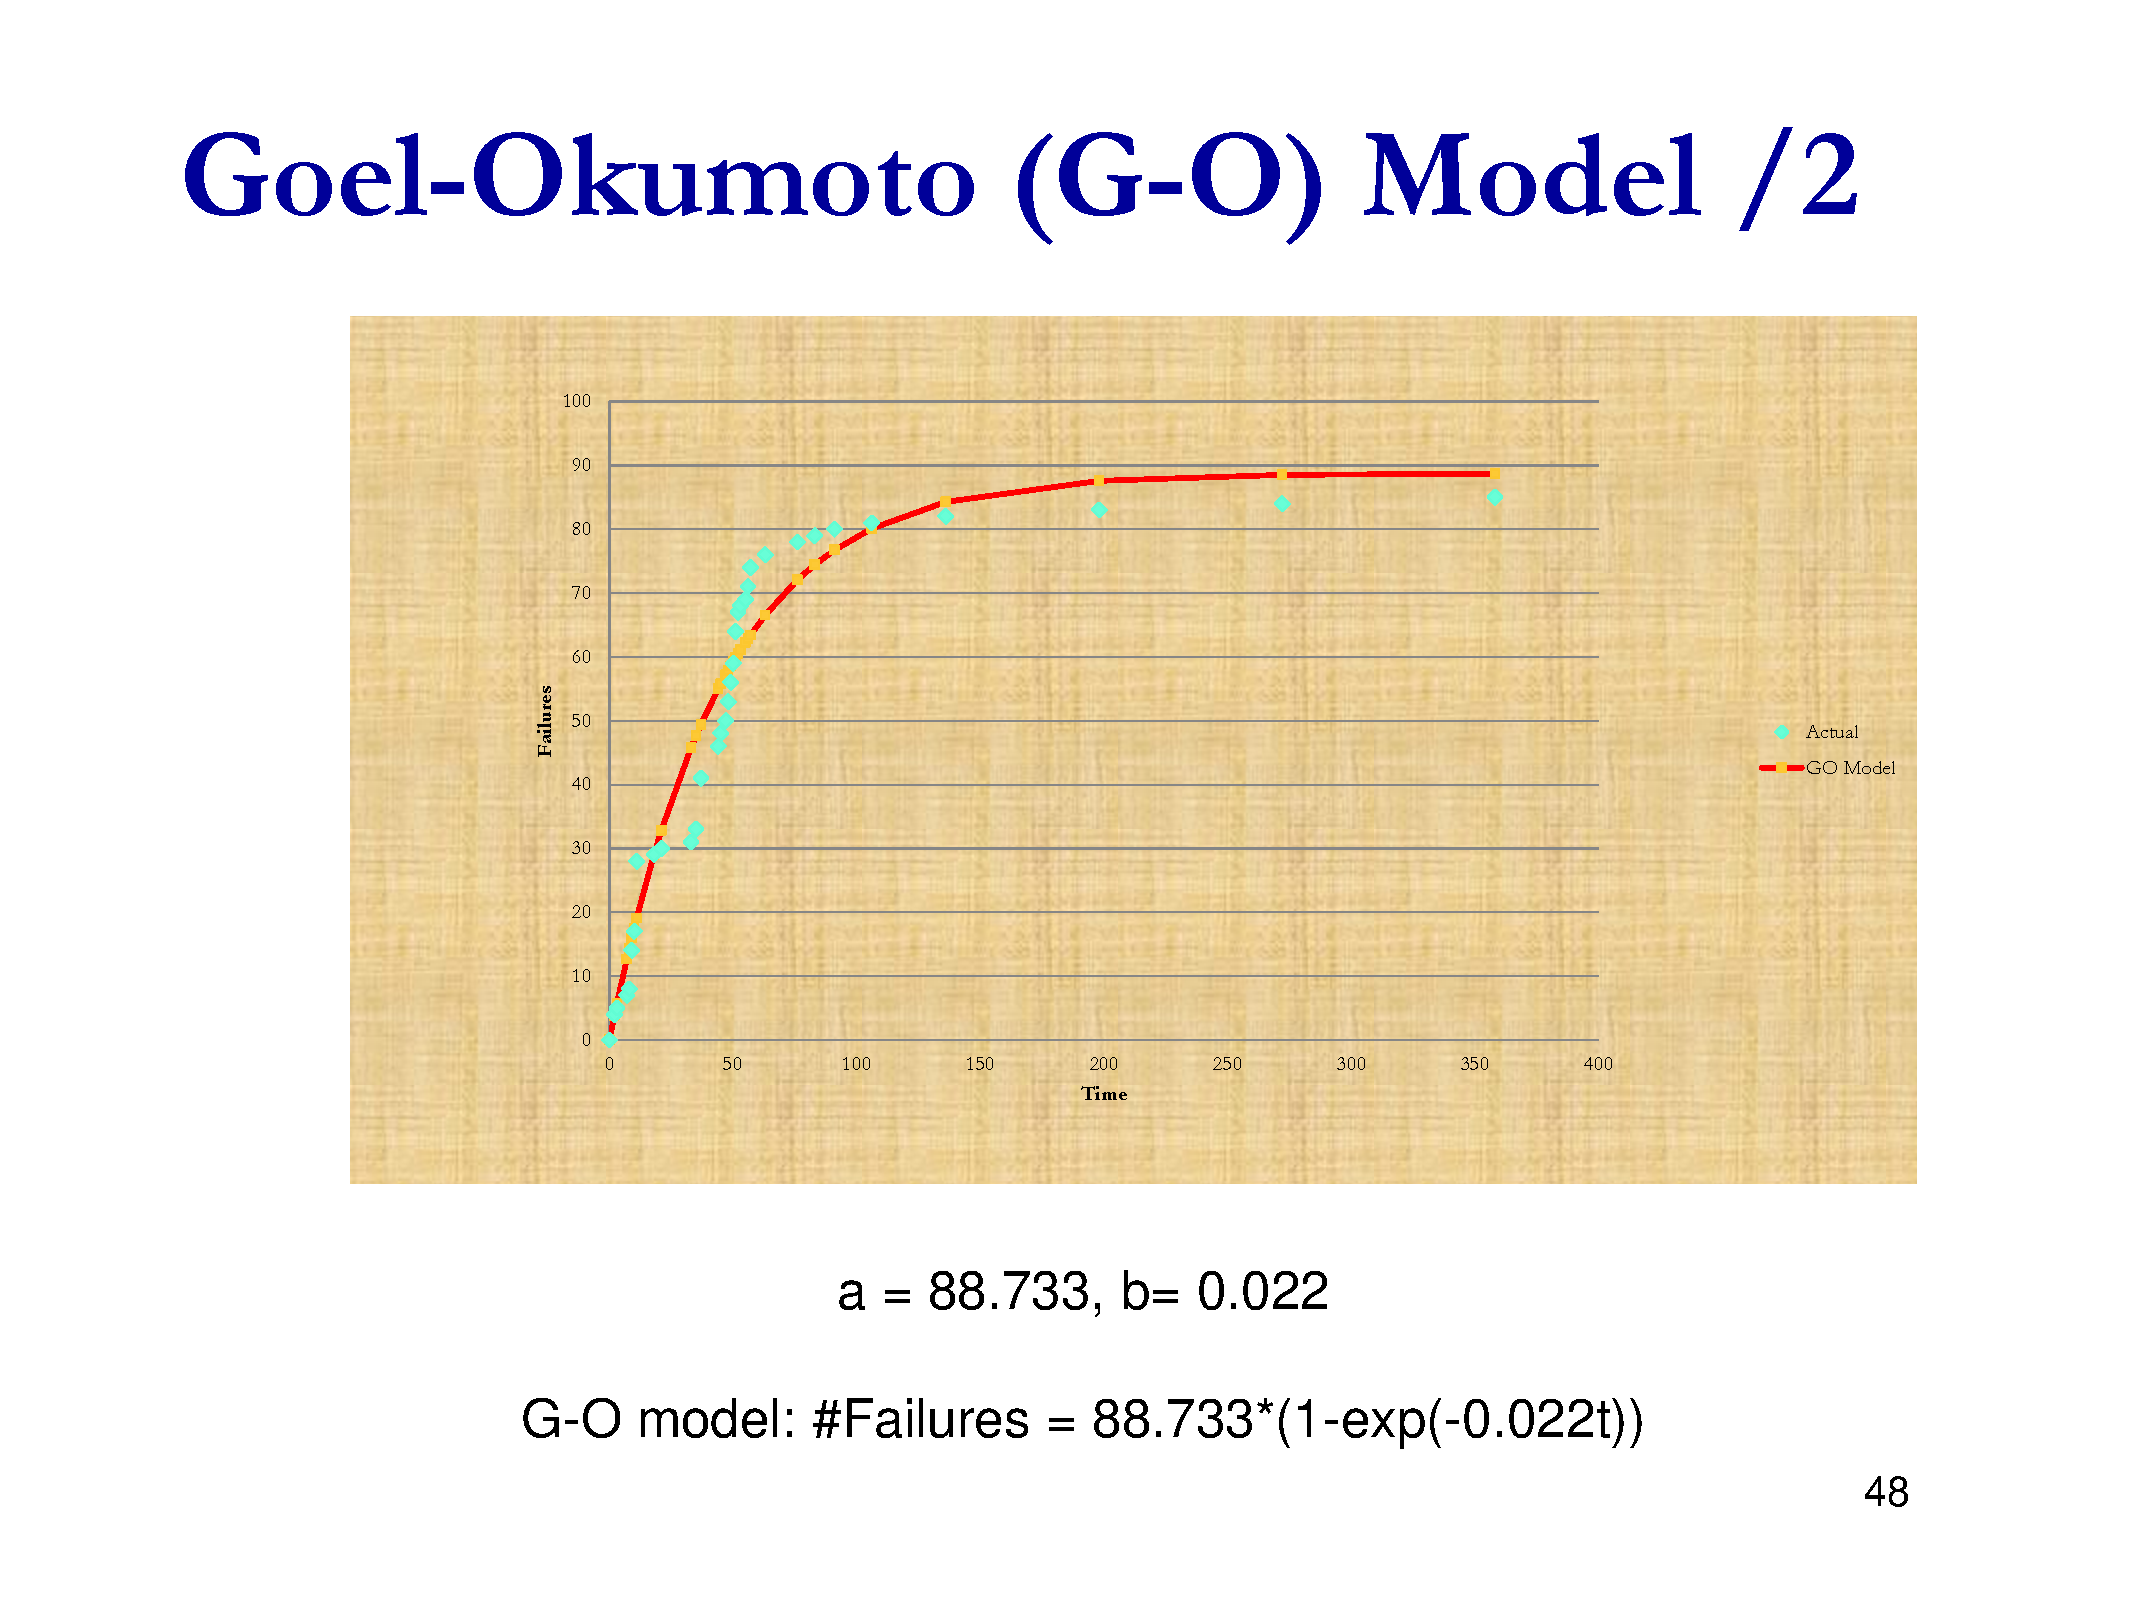
\includegraphics[width=\linewidth]{392.pdf}\\
        \textbf{Mean time to failure}: mean of probability density, expected value of T, average lifetime of system, $E(T) = \int_0^\infty t \: f(t)dt = \int_0^\infty R(t)dt$, for exponential is $\frac{1}{\lambda}$\\
        \textbf{Mean time between failures}: $MTTF + MTTR$ (mean time to repair)\\
        \textbf{Software reliability tools tasks}: collecting failure \& test time info, calculating estimates of model parameters using this onfo, testing to fit model against collected info, selecting model to make predictions of remaining faults, time to test, apply model\\
        \vfill\null\columnbreak\noindent\underline{\textbf{Week 9}}\\
        \textbf{Software reviews}: quality improvement processes for written material, by detecting defects early \& preventing leakage downstream higher cost of later detection \& rework eliminated\\
        \textbf{Software products that can be reviewed}: requirements specifications, design descriptions, source code (code review), release notes\\
        \textbf{Code review types}: ad-hoc review, pass-round, walkthrough, group review, formal inspection\\
        \textbf{Formal Inspection}: planning/overview, preparation (product docs, rules/checklist), inspection, rework\\
        \textbf{Code review steps}: perform examination of software products, detect defects (bugs), violation of coding standards, code smells, other problems, look for code patterns that indicate problems based on prior xp, static analysis tools can also help\\
        \textbf{Bug patterns}: infinite recursion, null pointer bugs, SQL injection, divide by 0, buffer overflow, memory leak, deadlock, infinite loop, XSS\\
        \textbf{\textbf{Code smells}}: indications of poor coding \& design choices that can cause problems during later phase of development, hint something gone wrong somewhere
        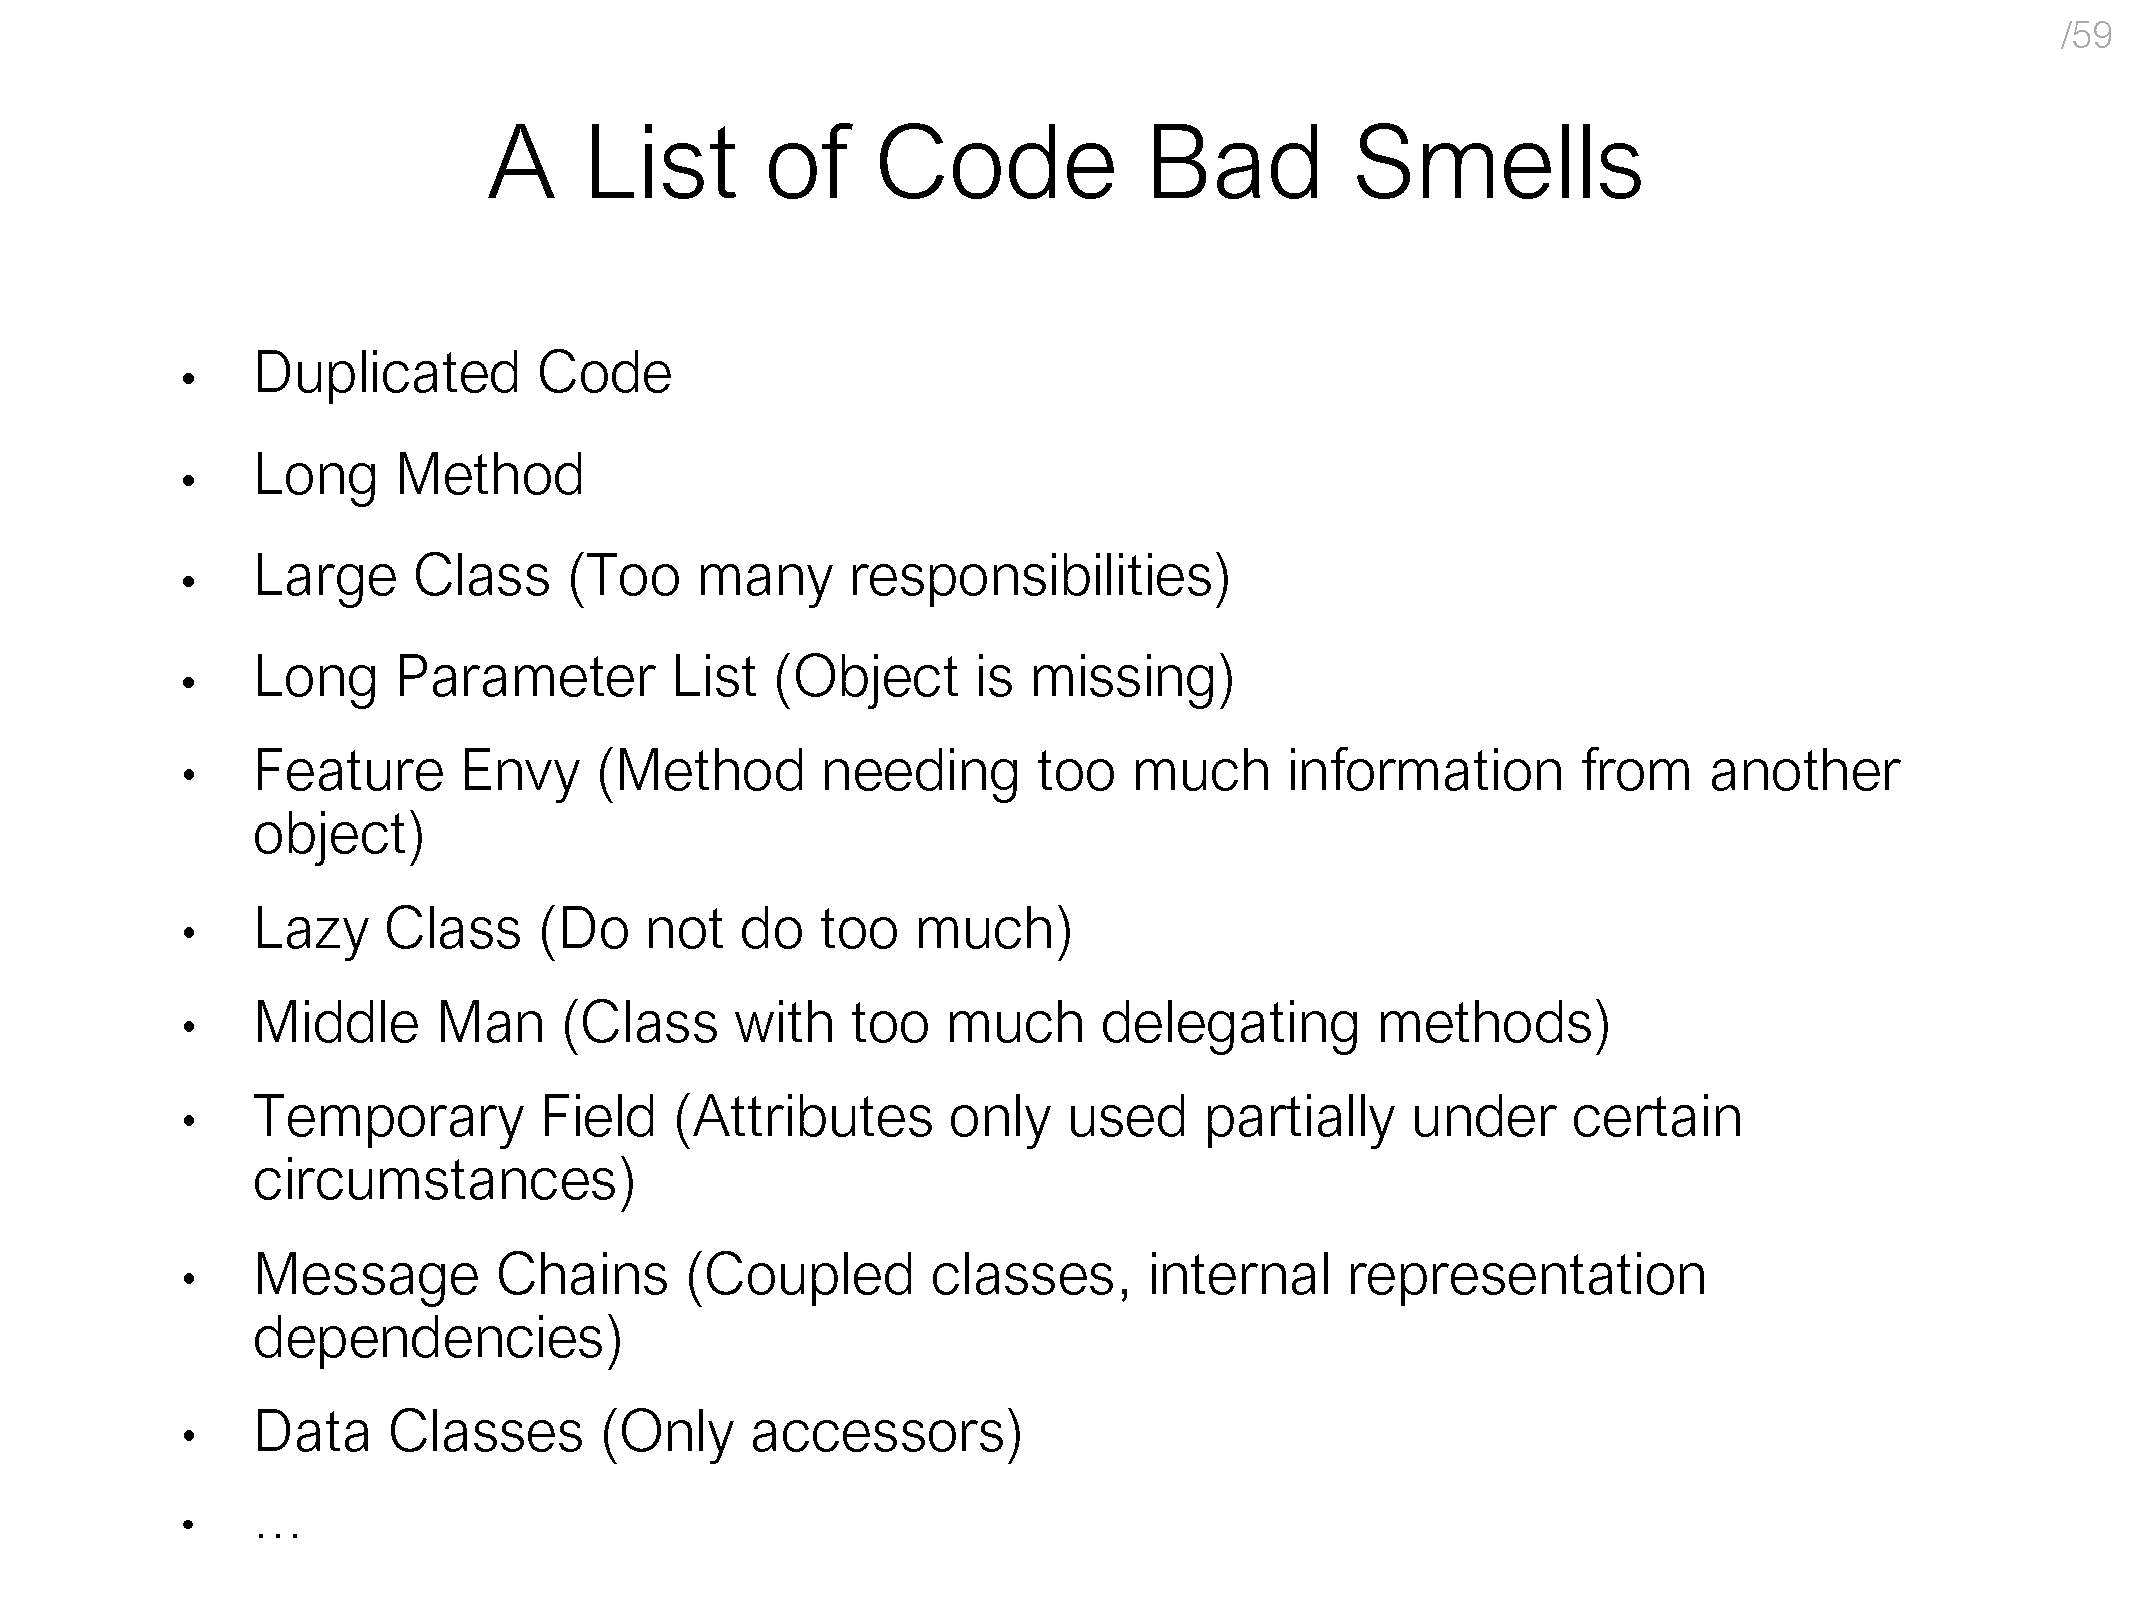
\includegraphics[width=\linewidth]{418.pdf}\\
        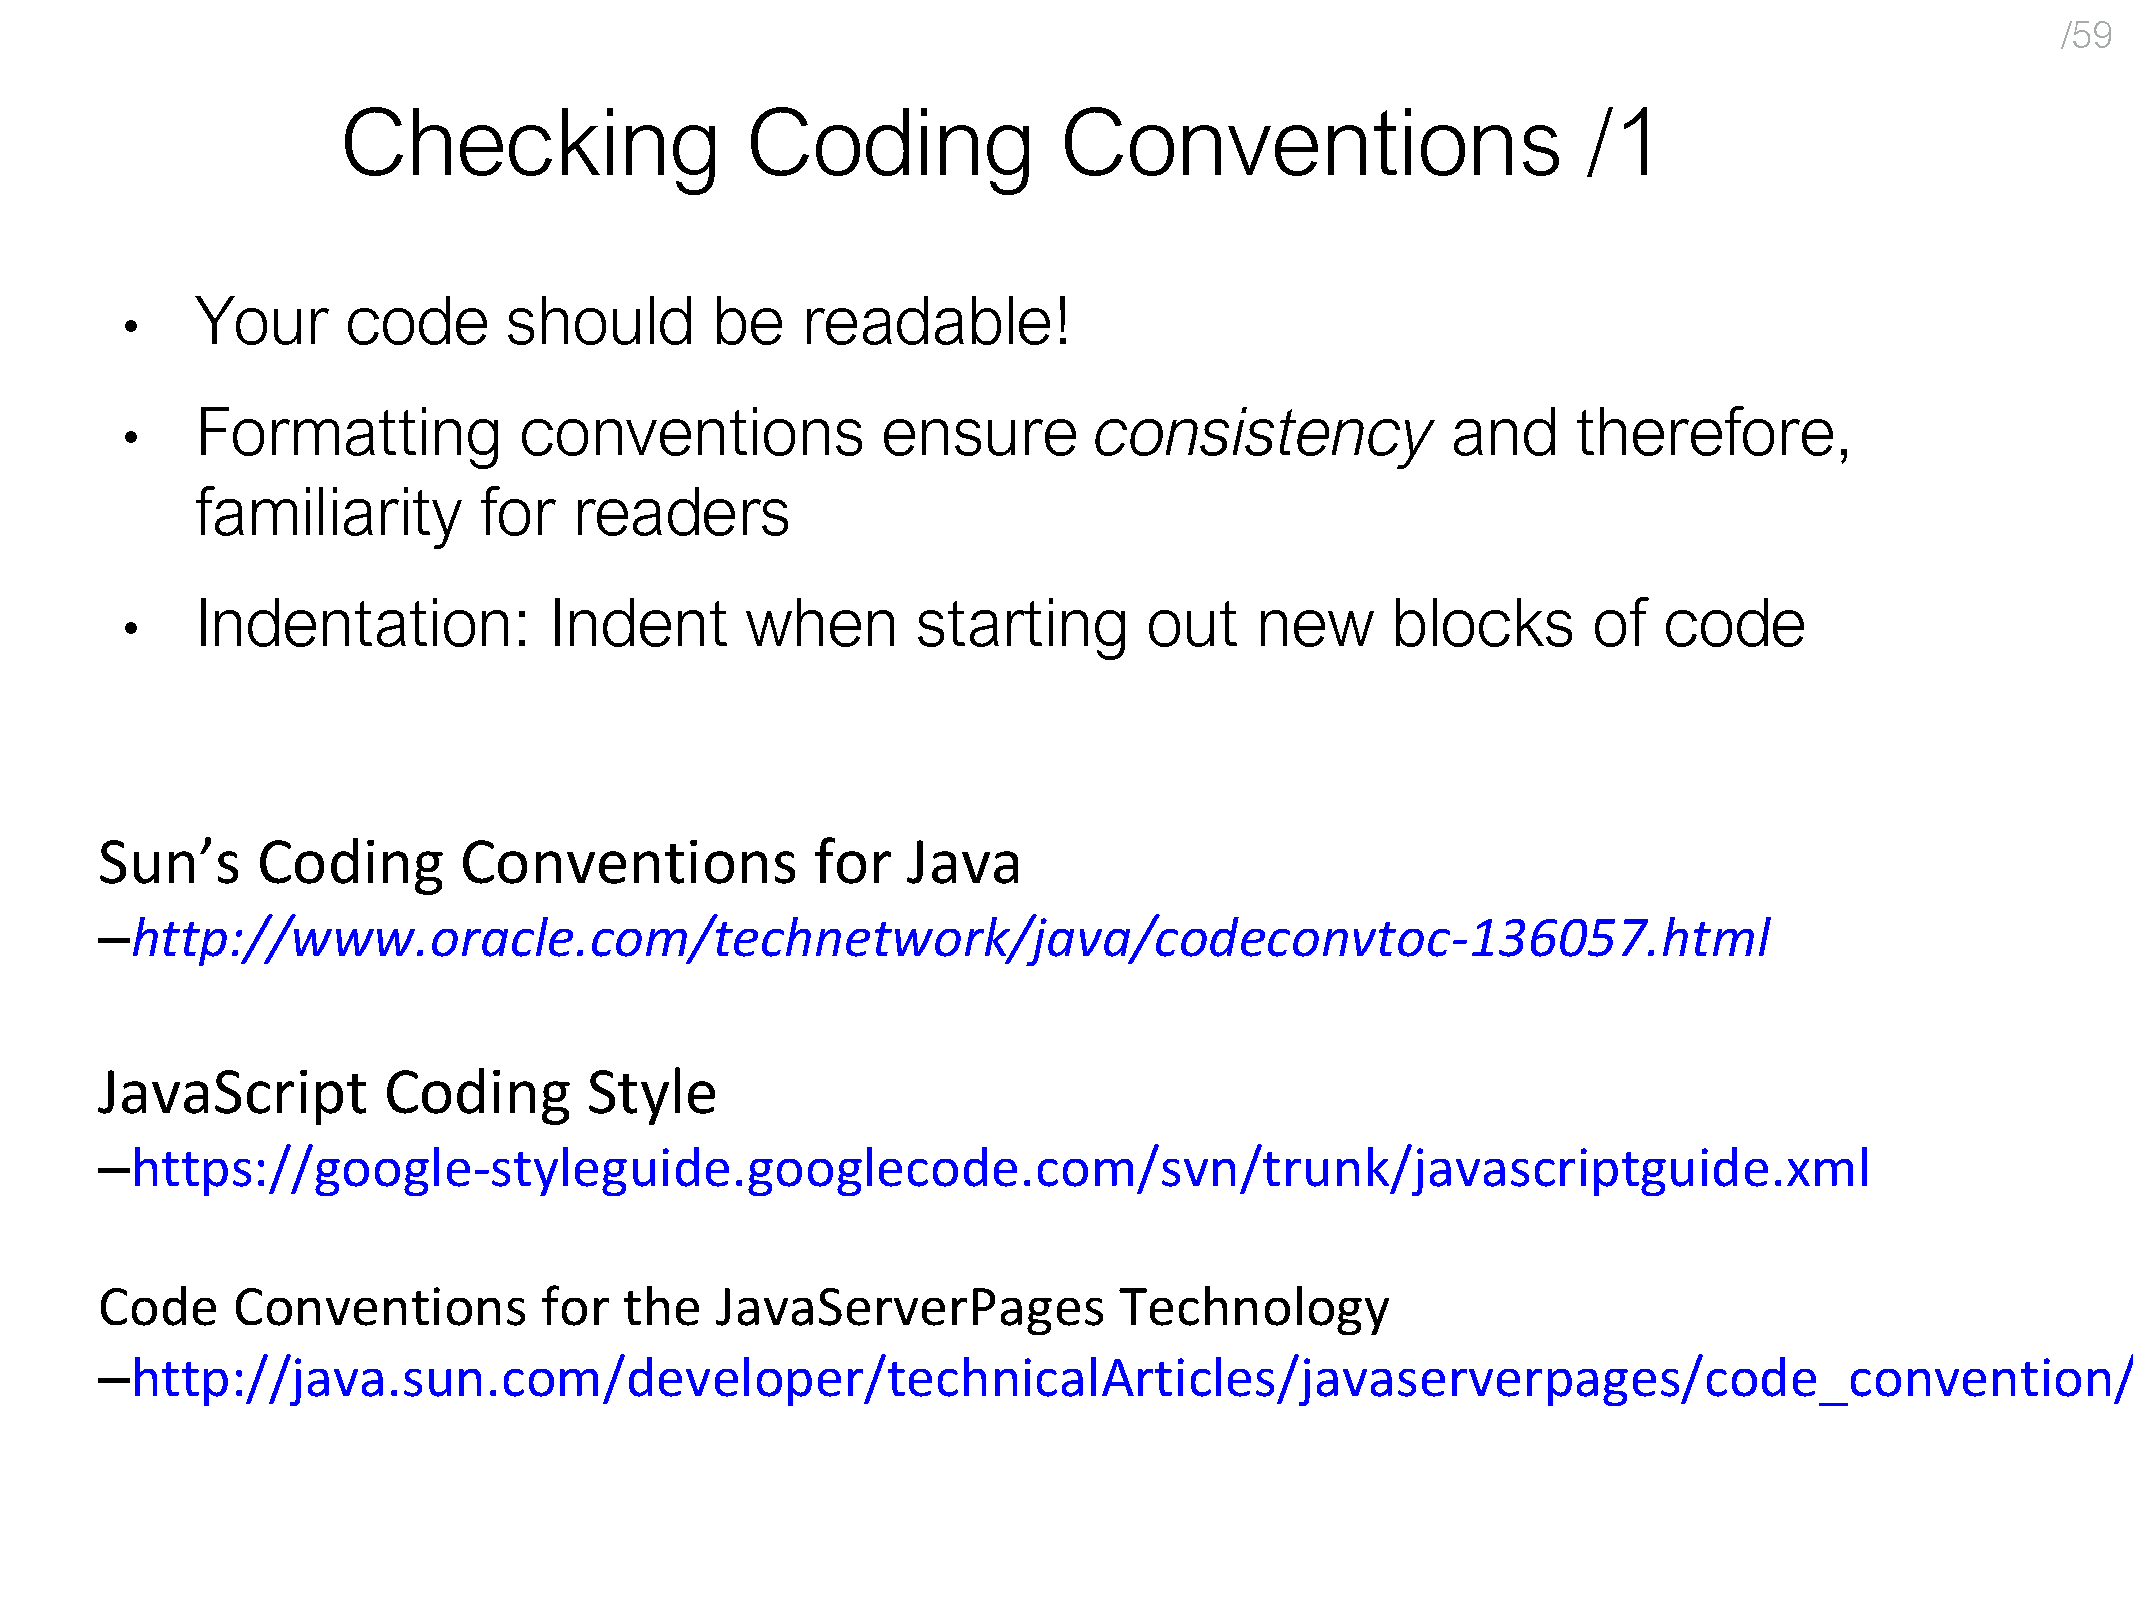
\includegraphics[width=\linewidth]{419.pdf}\\
        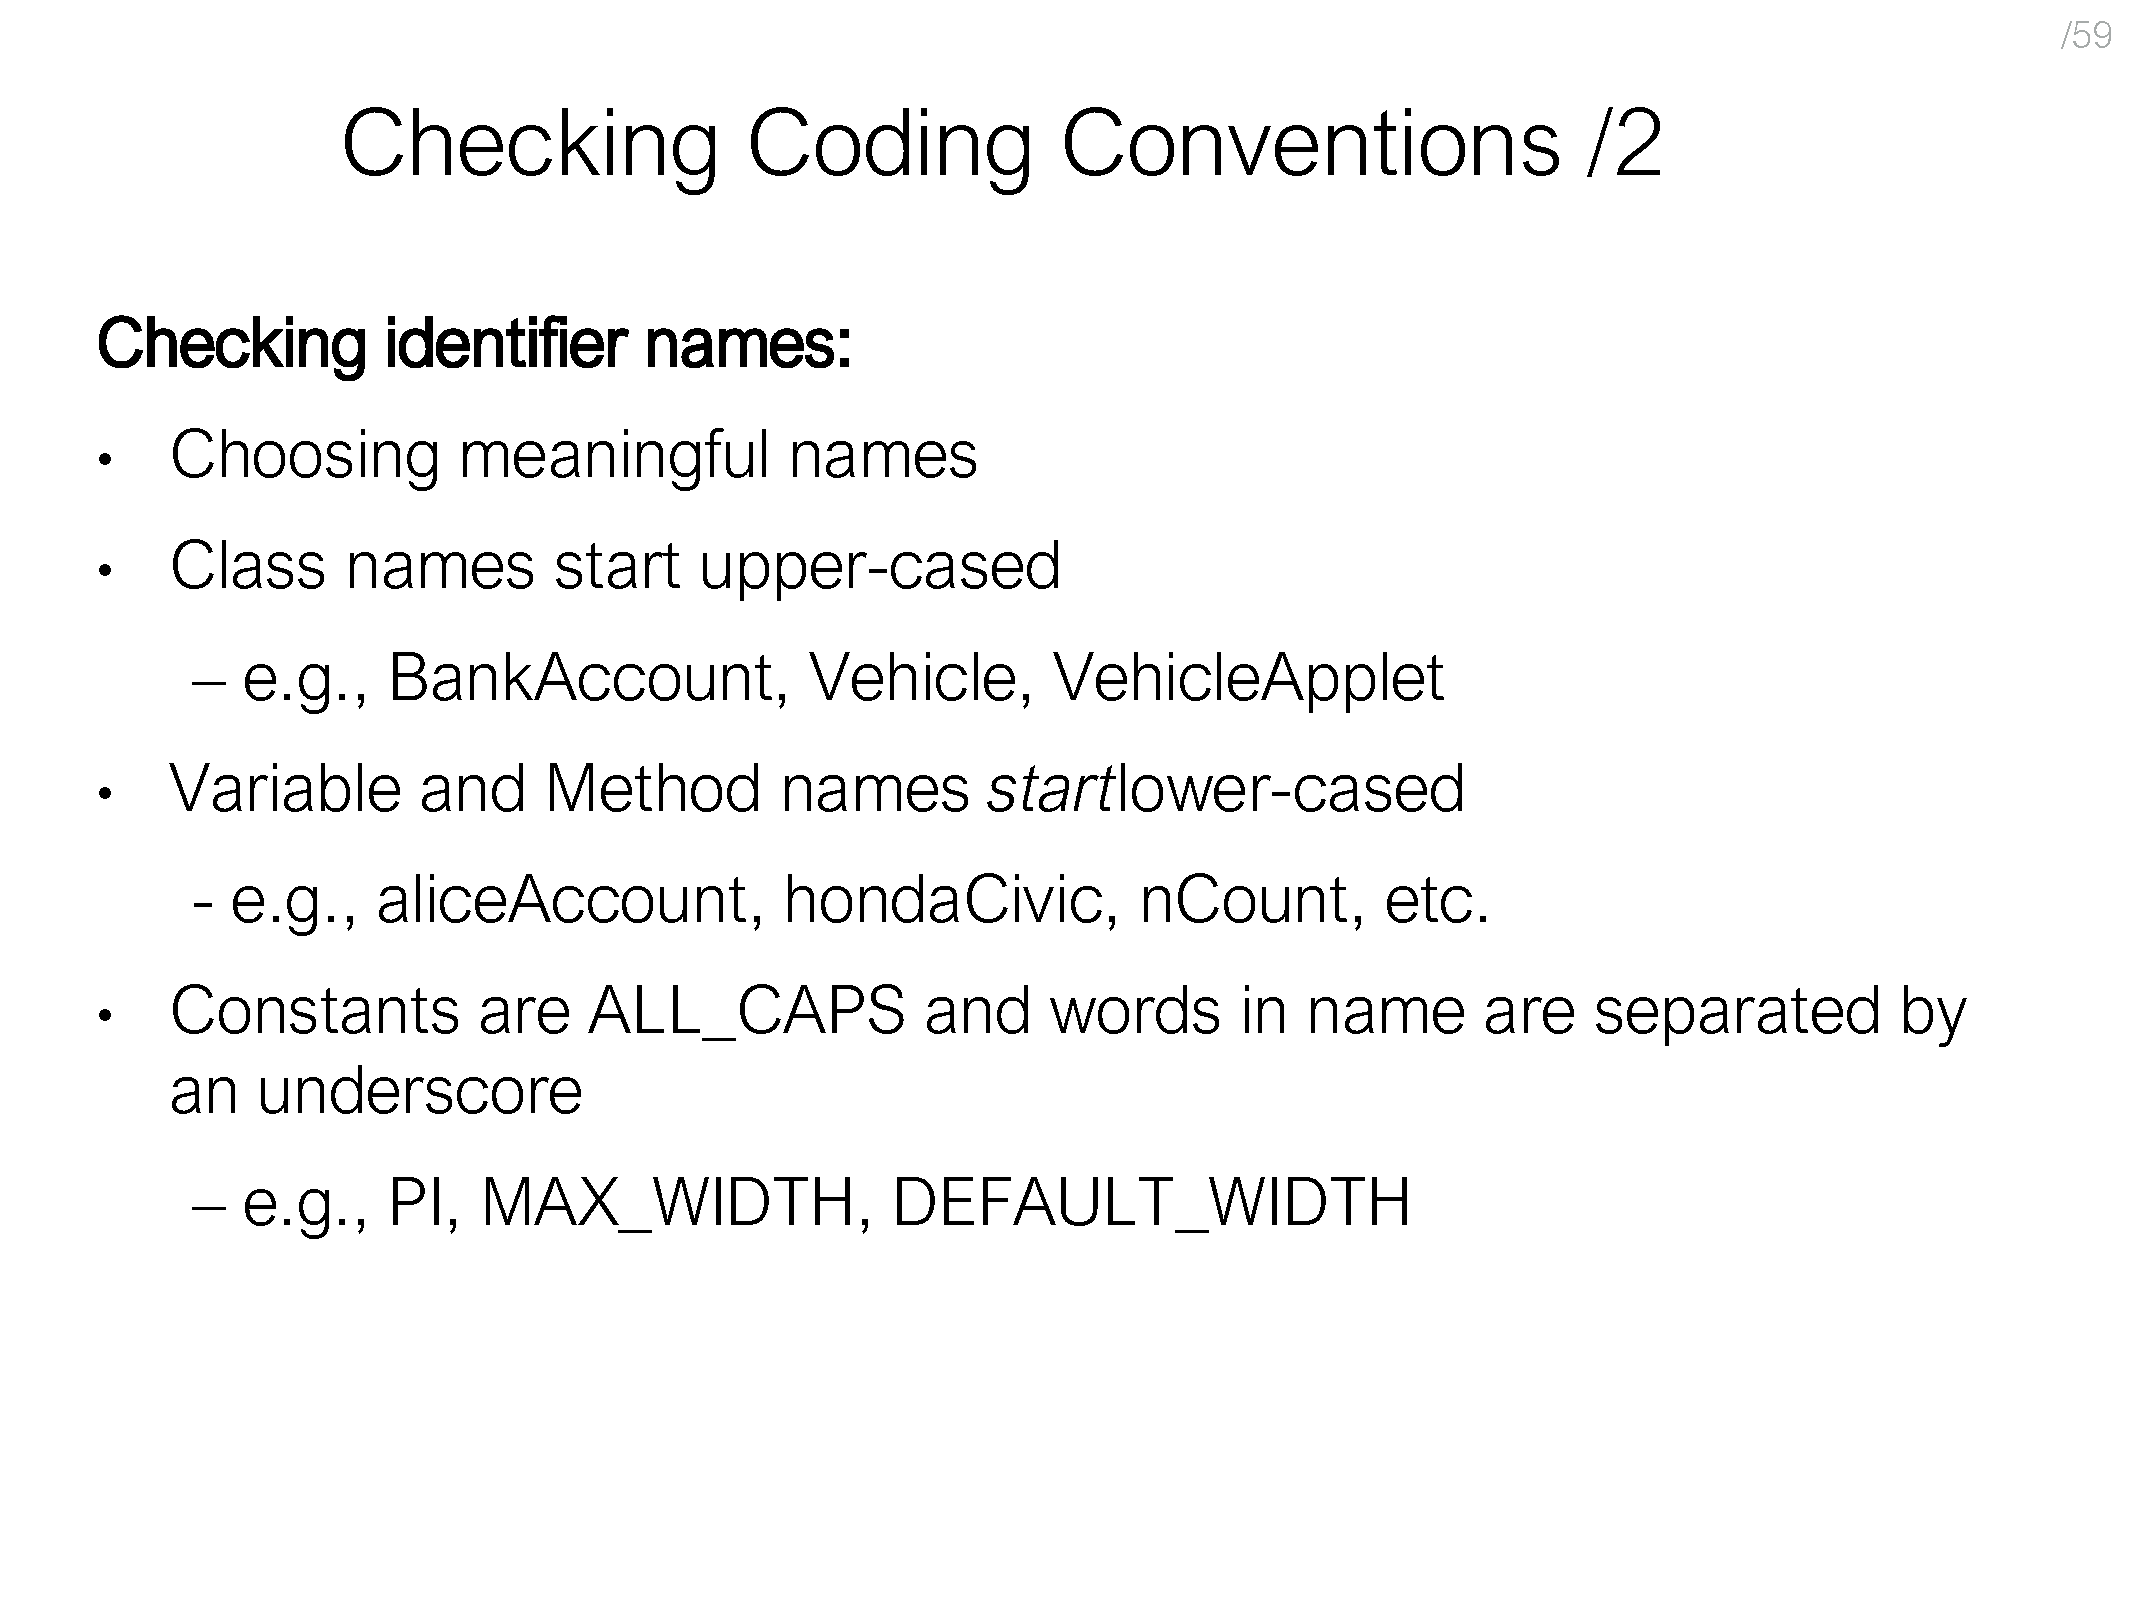
\includegraphics[width=\linewidth]{420.pdf}\\
        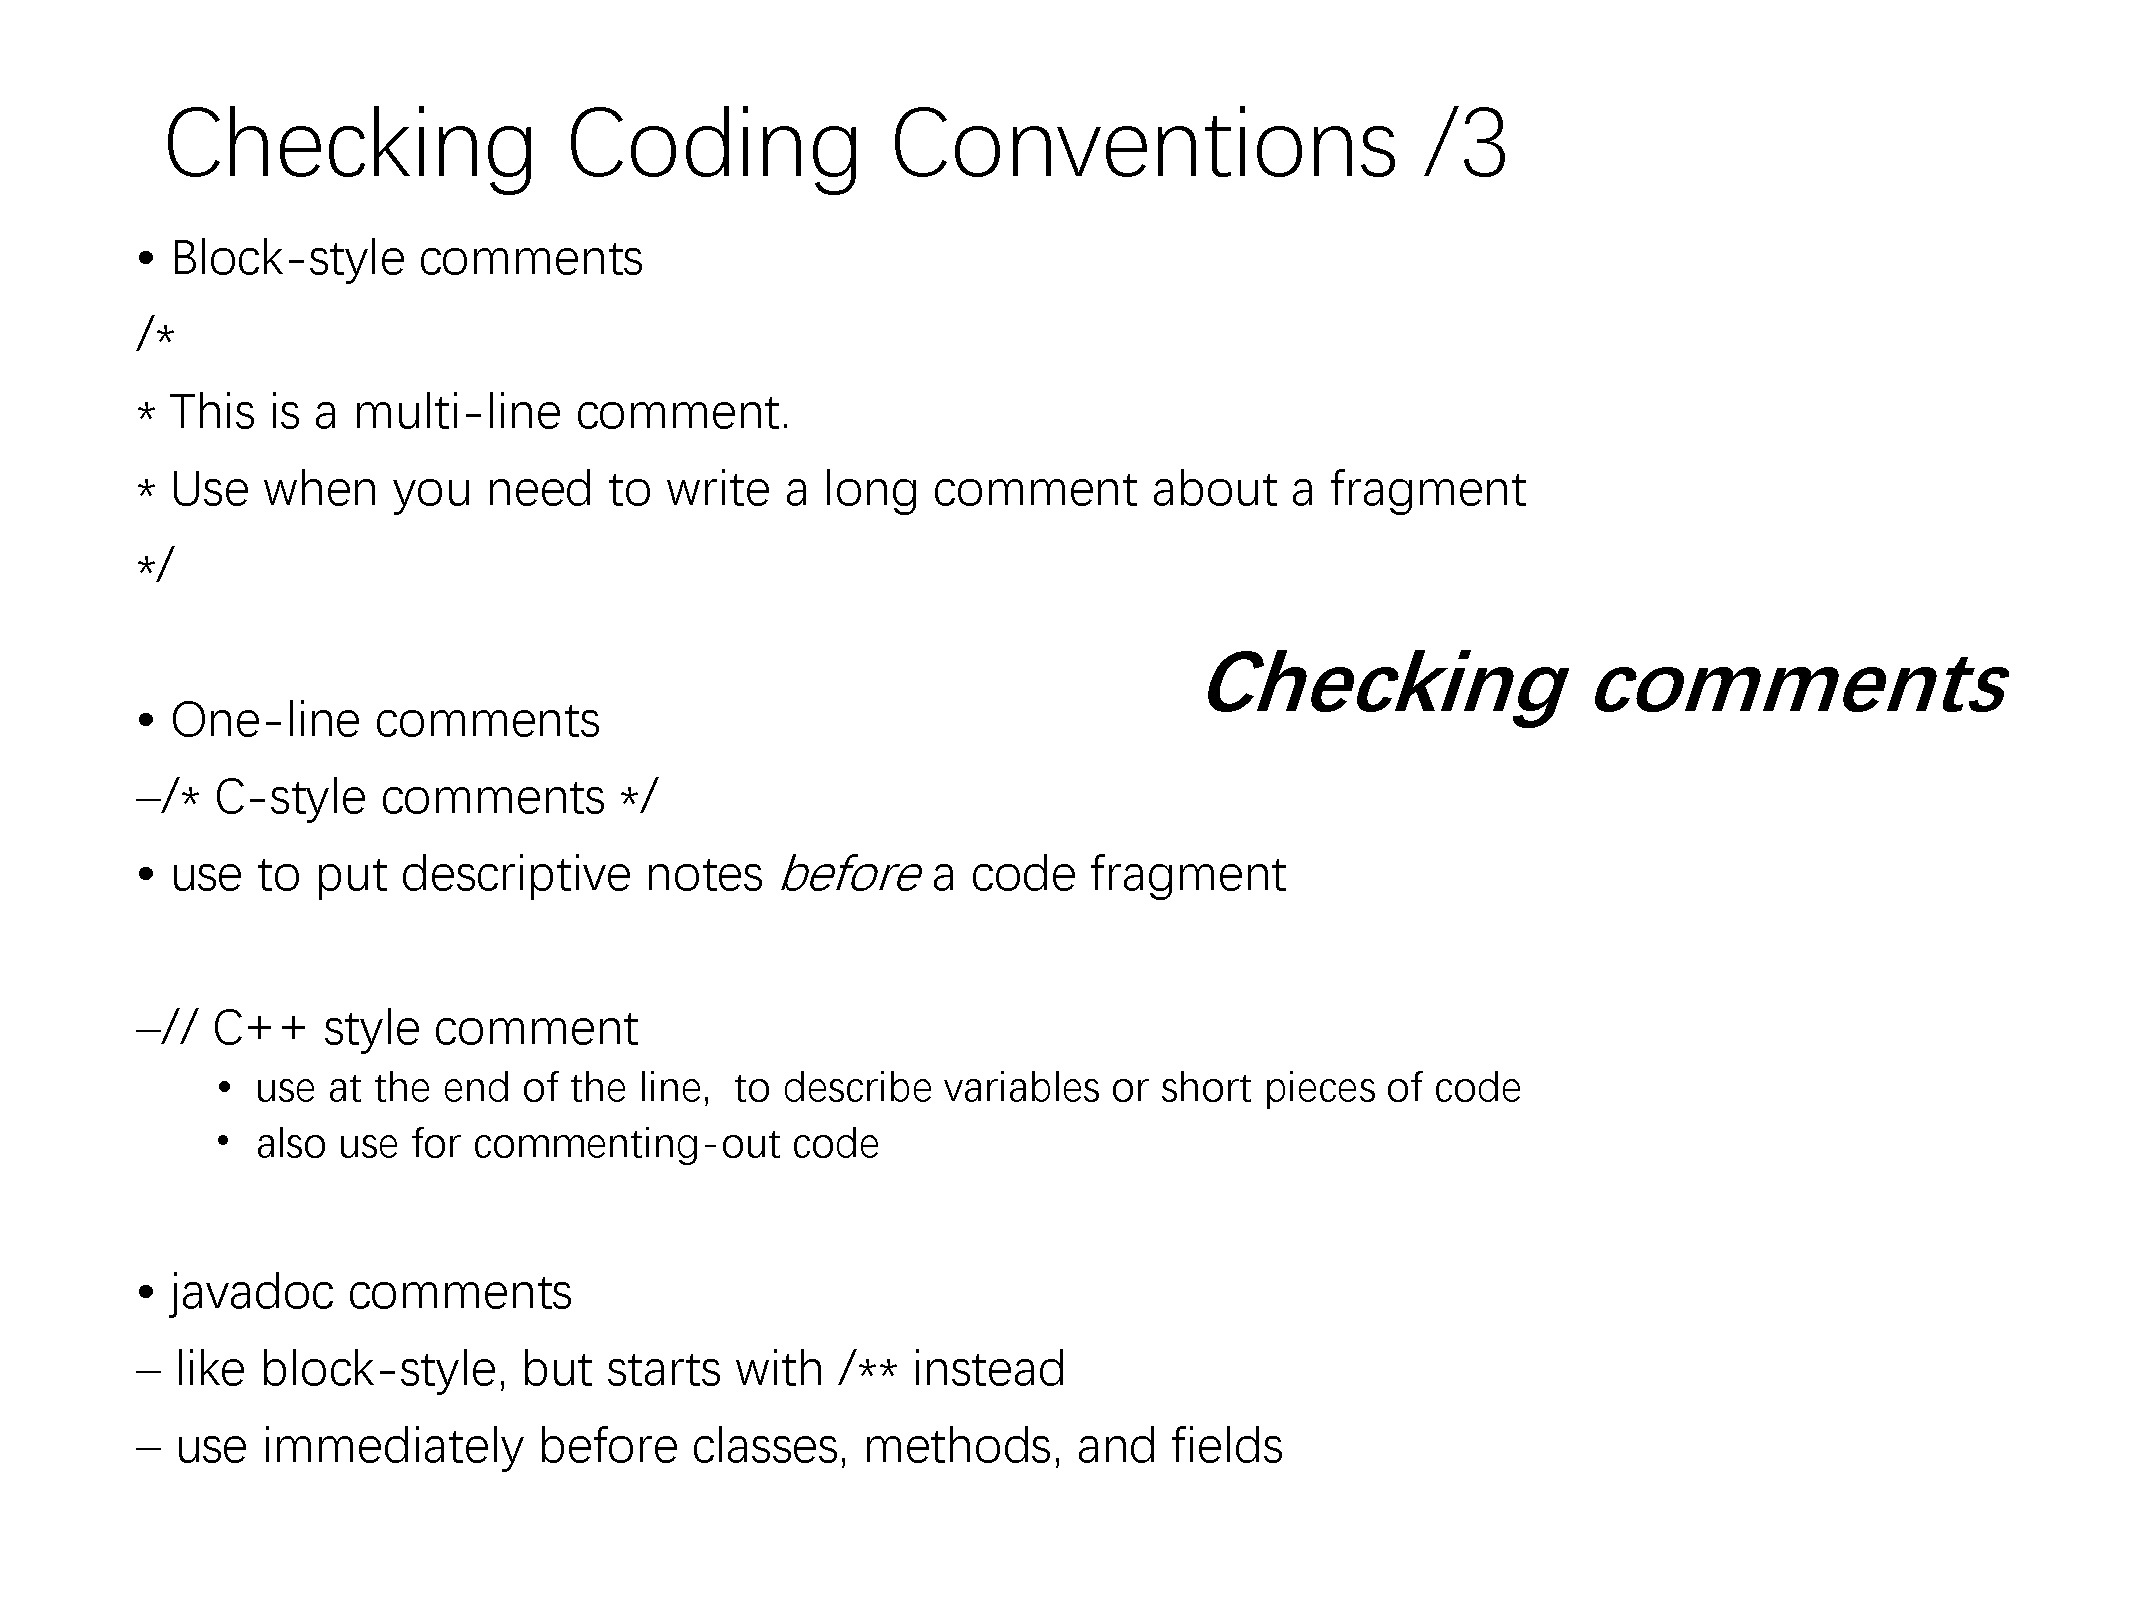
\includegraphics[width=\linewidth]{421.pdf}\\
        \textbf{Code Review benefits}: can find 60--100\% of defects, can assess/improve quality of work product, software development process \& review process itself, reduce total project cost but have non-trivial cost (15\%), early defect removal is 10--100 times cheaper, reviews distribute domain knowledge, dev skills, corporate culture\\
        \textbf{Common problems in code review}: insufficient preparation, moderator domination, incorrect review rate, ego involvement \& personality conflict, issue resolution \& meeting digression,recording difficulties \& clerical overhead\\
        \textbf{Static Analysis}: analyse program without executing, doesn't depend on test cases, generally doesn't know what the software is supposed to do, looks for bug patterns, no replacement for testing, many defects can't be found with static analysis\\
        \textbf{Patterns to be checked}: bad practice, correctness, performance, dodgy code, vulnerability to malicious code\\
        \textbf{Pattern examples}: equals method should not assume type of object argument, collection should not contain themselves ($!s.contains(s)$), should not use $String.toString()$\\
        \vfill\null\columnbreak\noindent\underline{\textbf{Week 10}}\\
        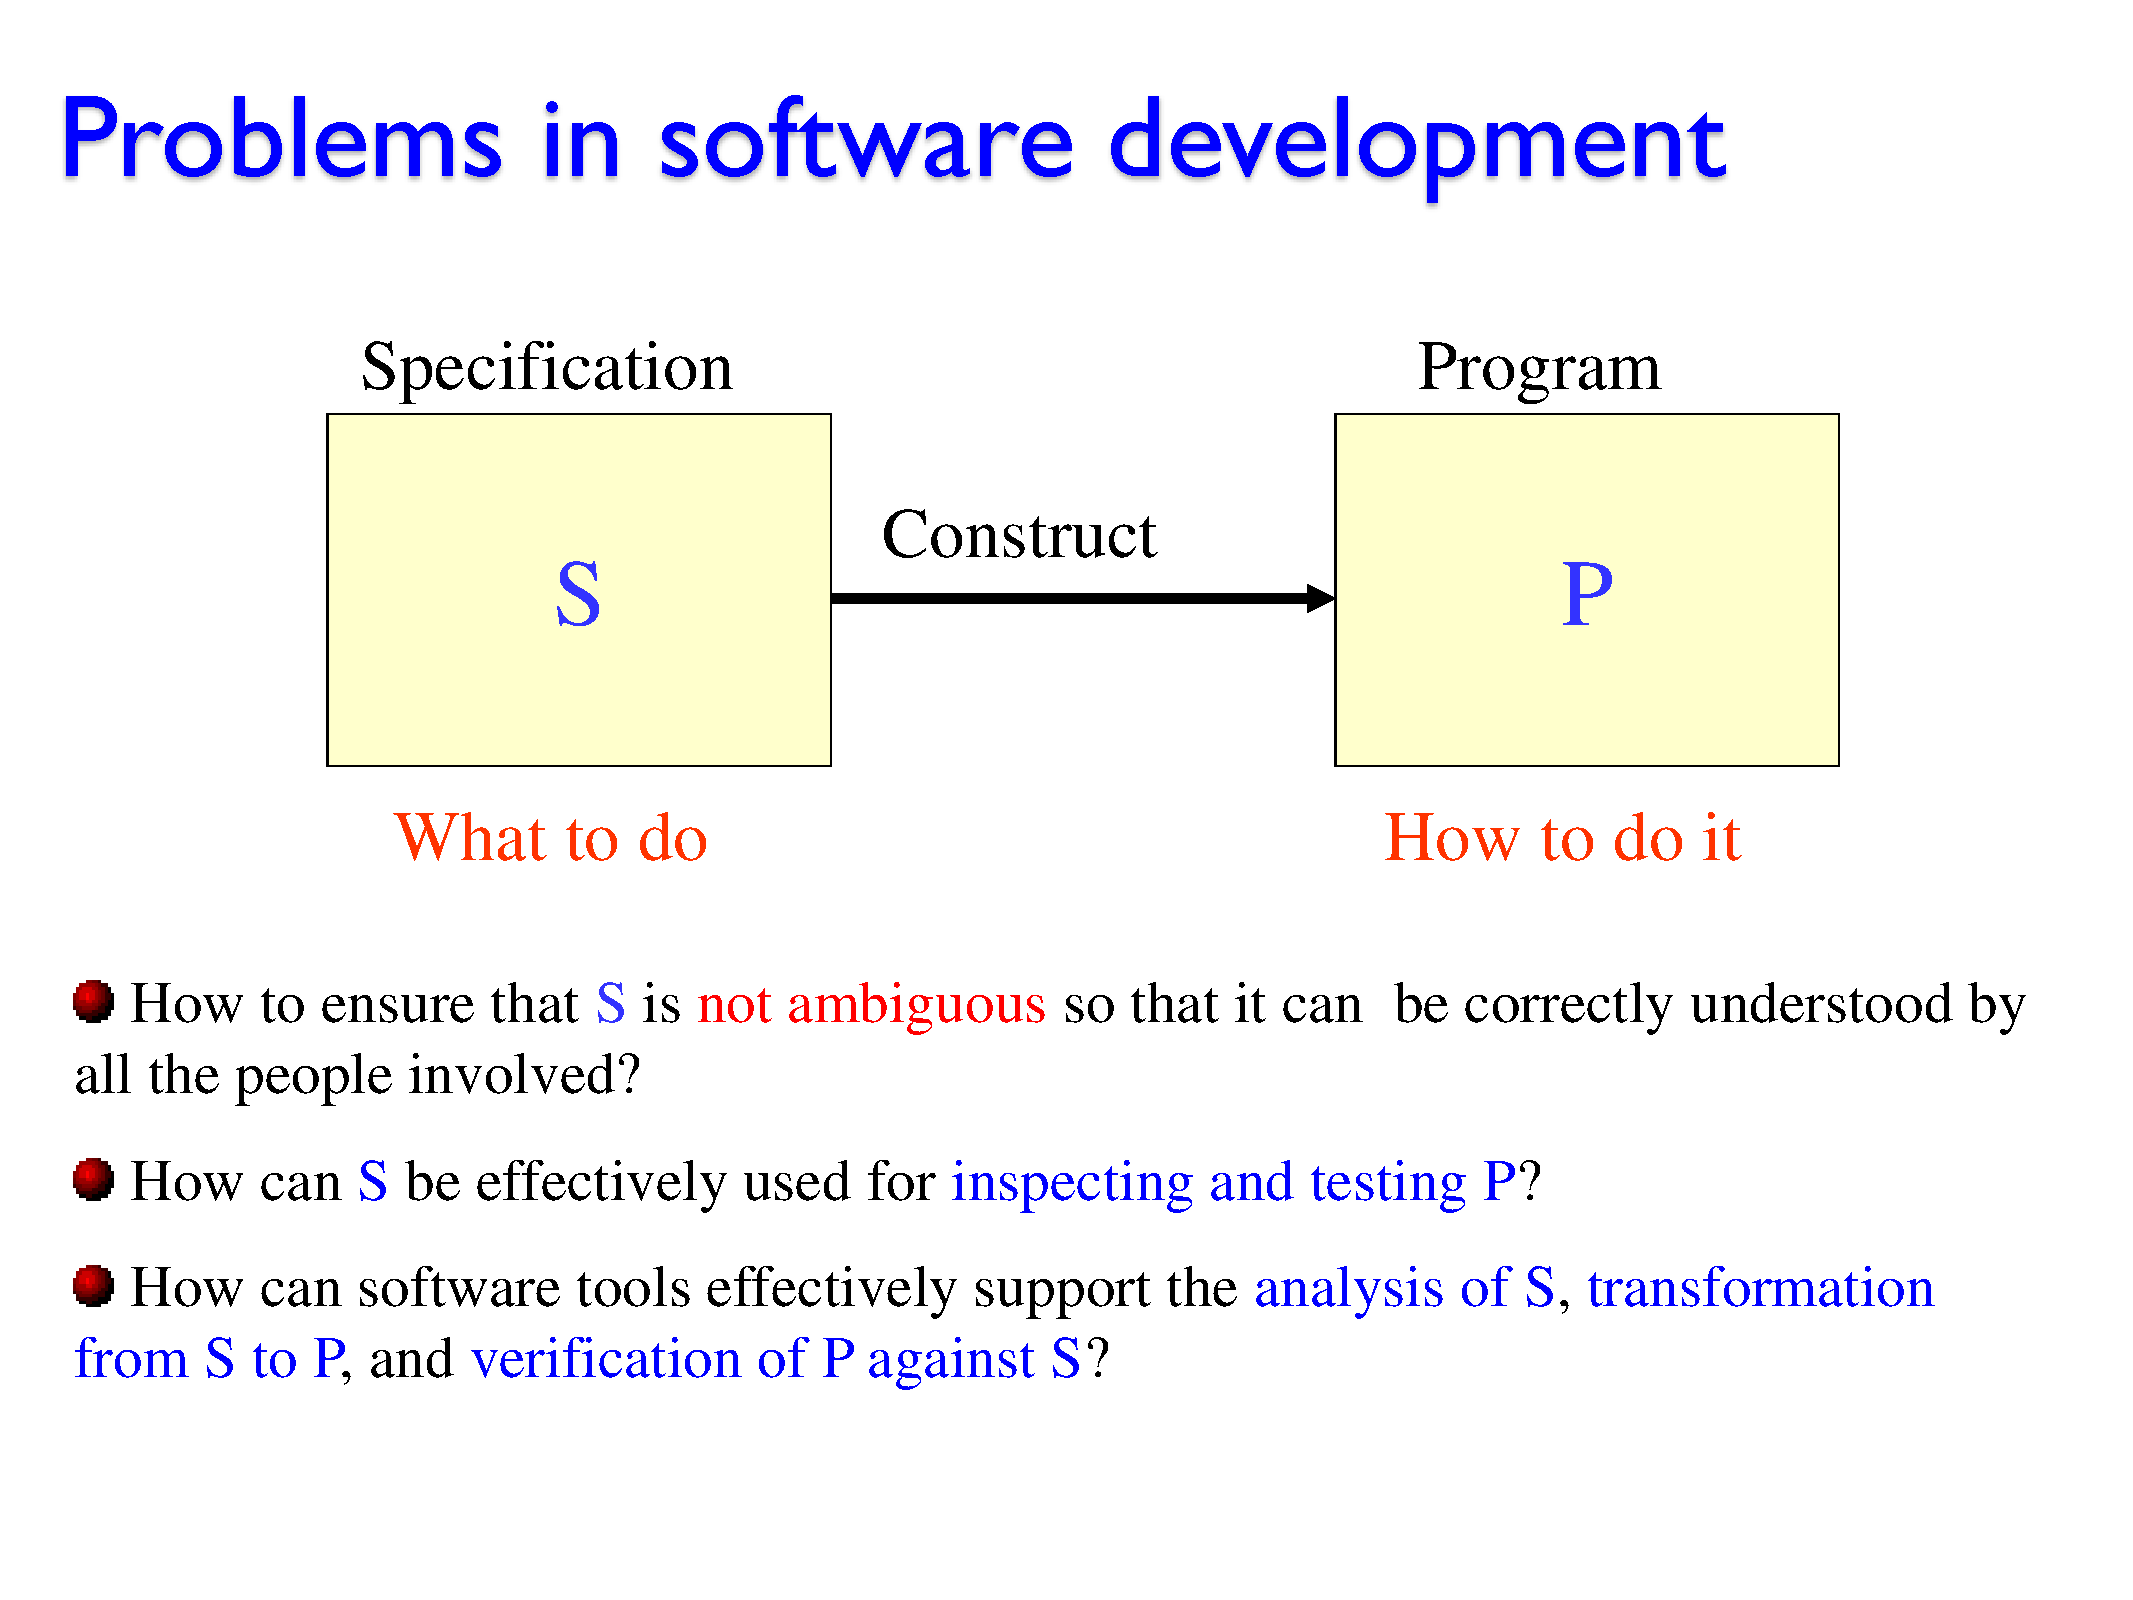
\includegraphics[width=\linewidth]{435.pdf}\\
        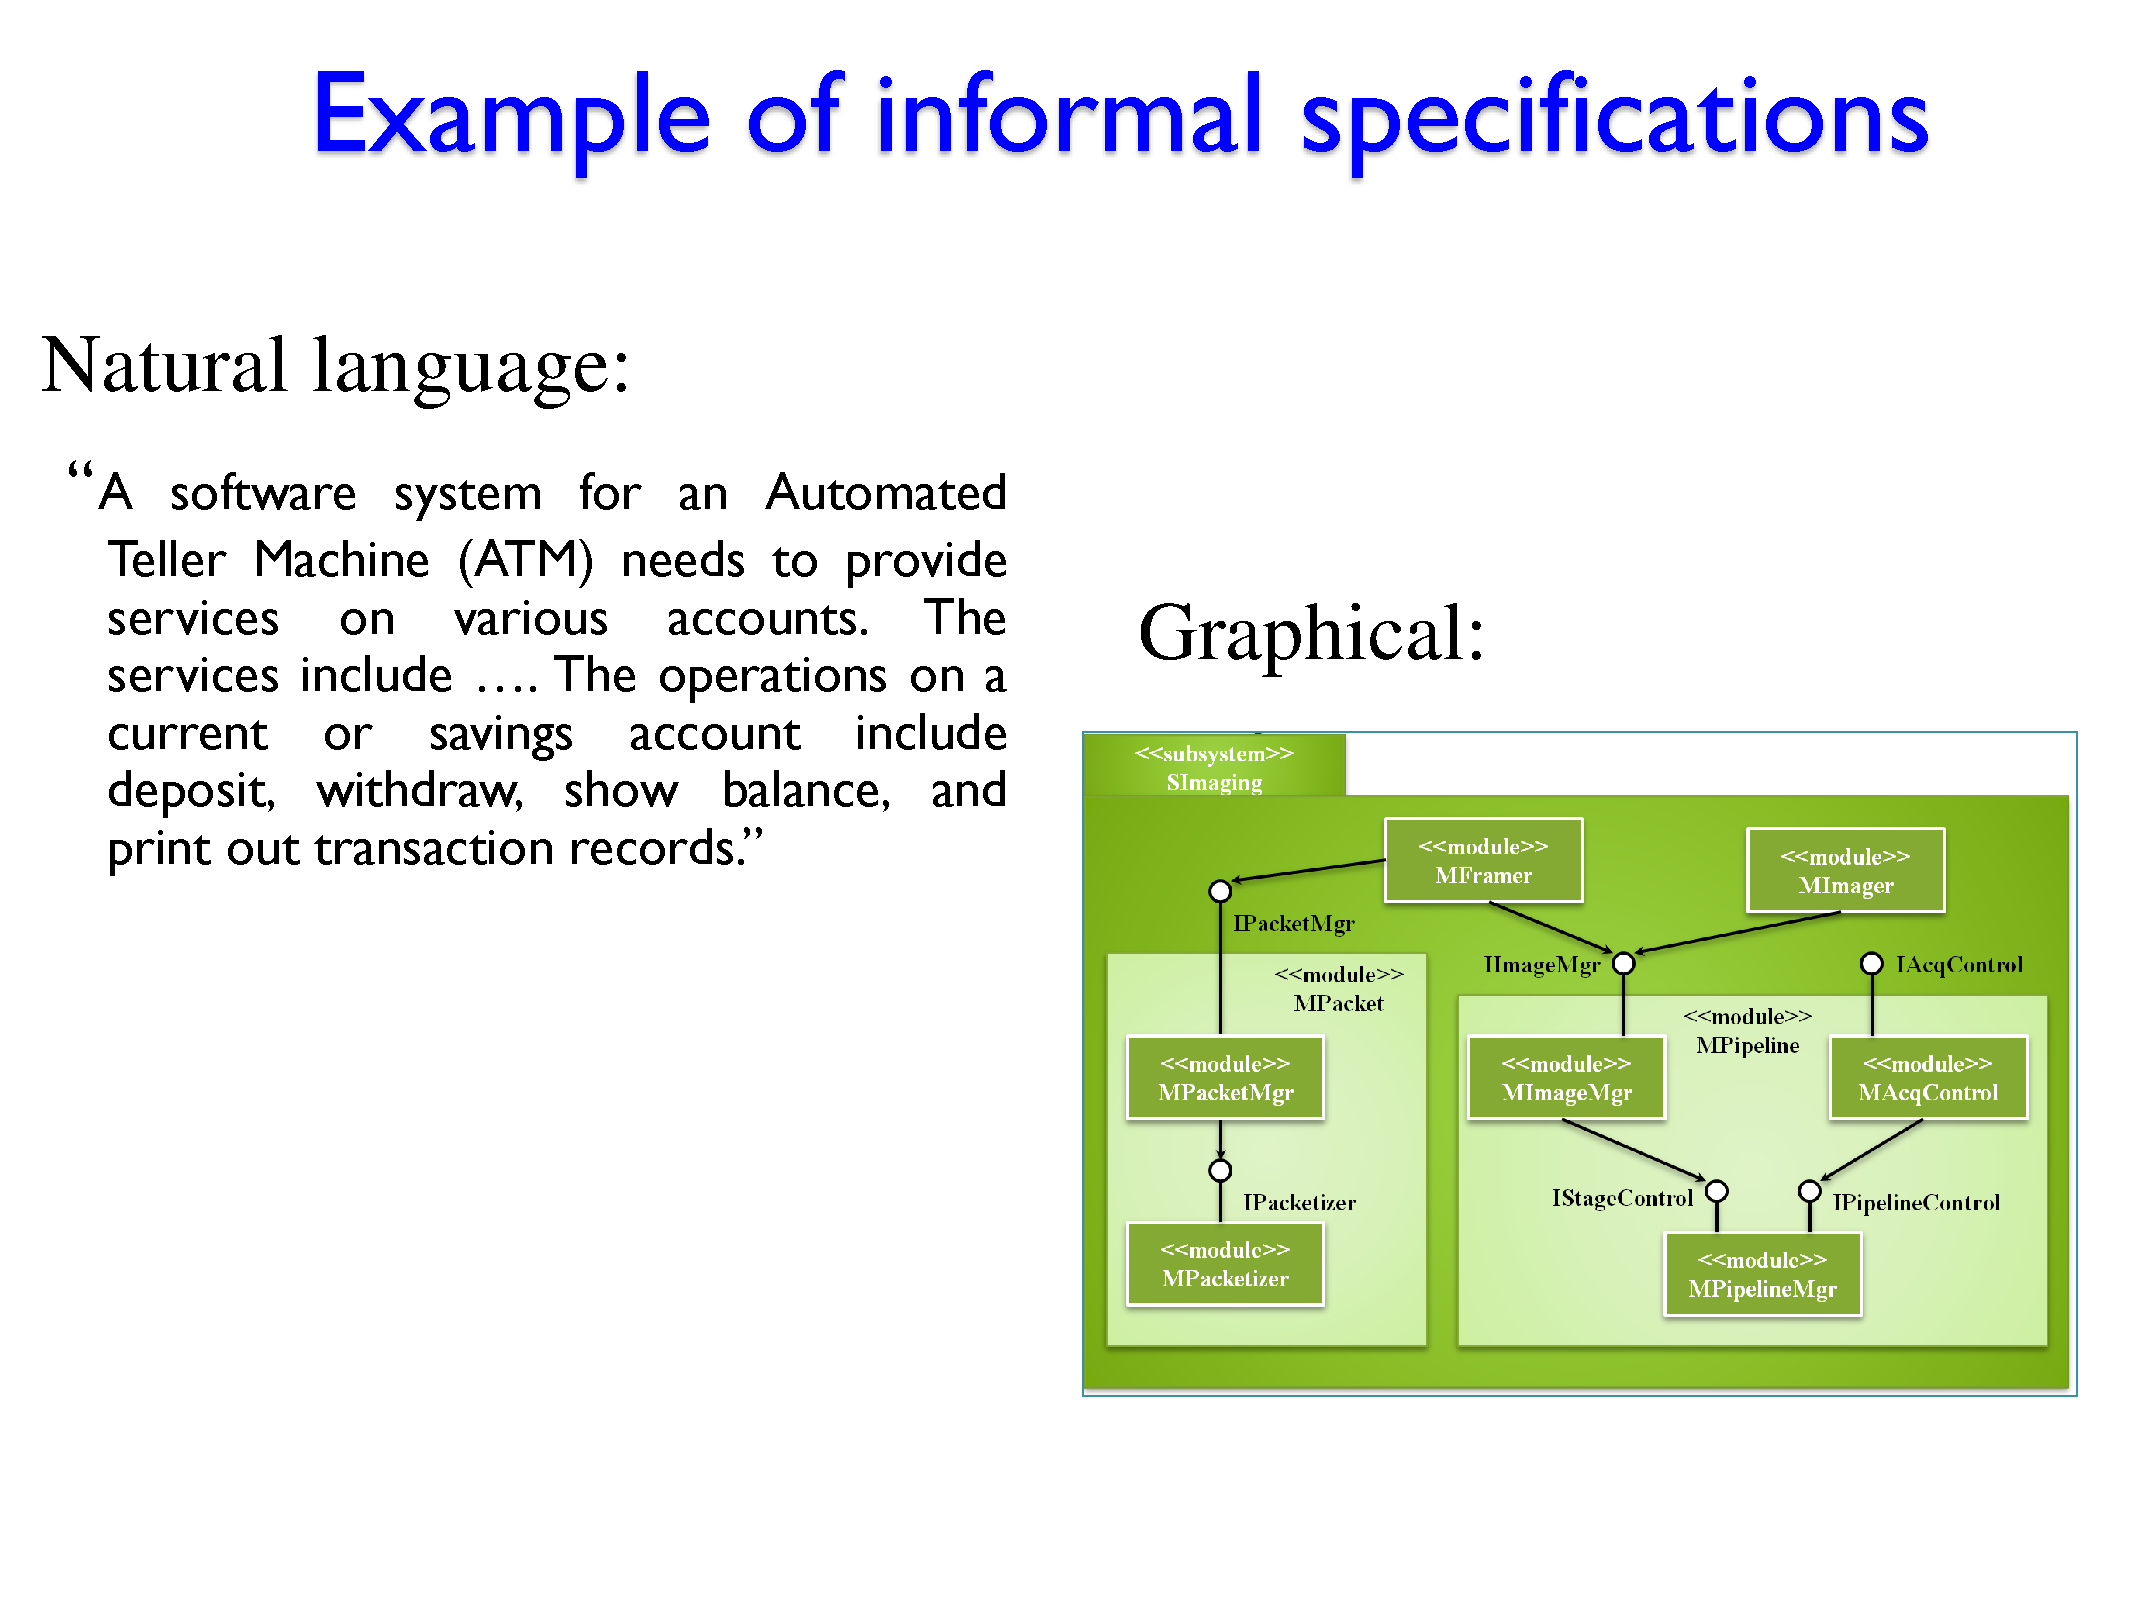
\includegraphics[width=\linewidth]{436.pdf}\\
        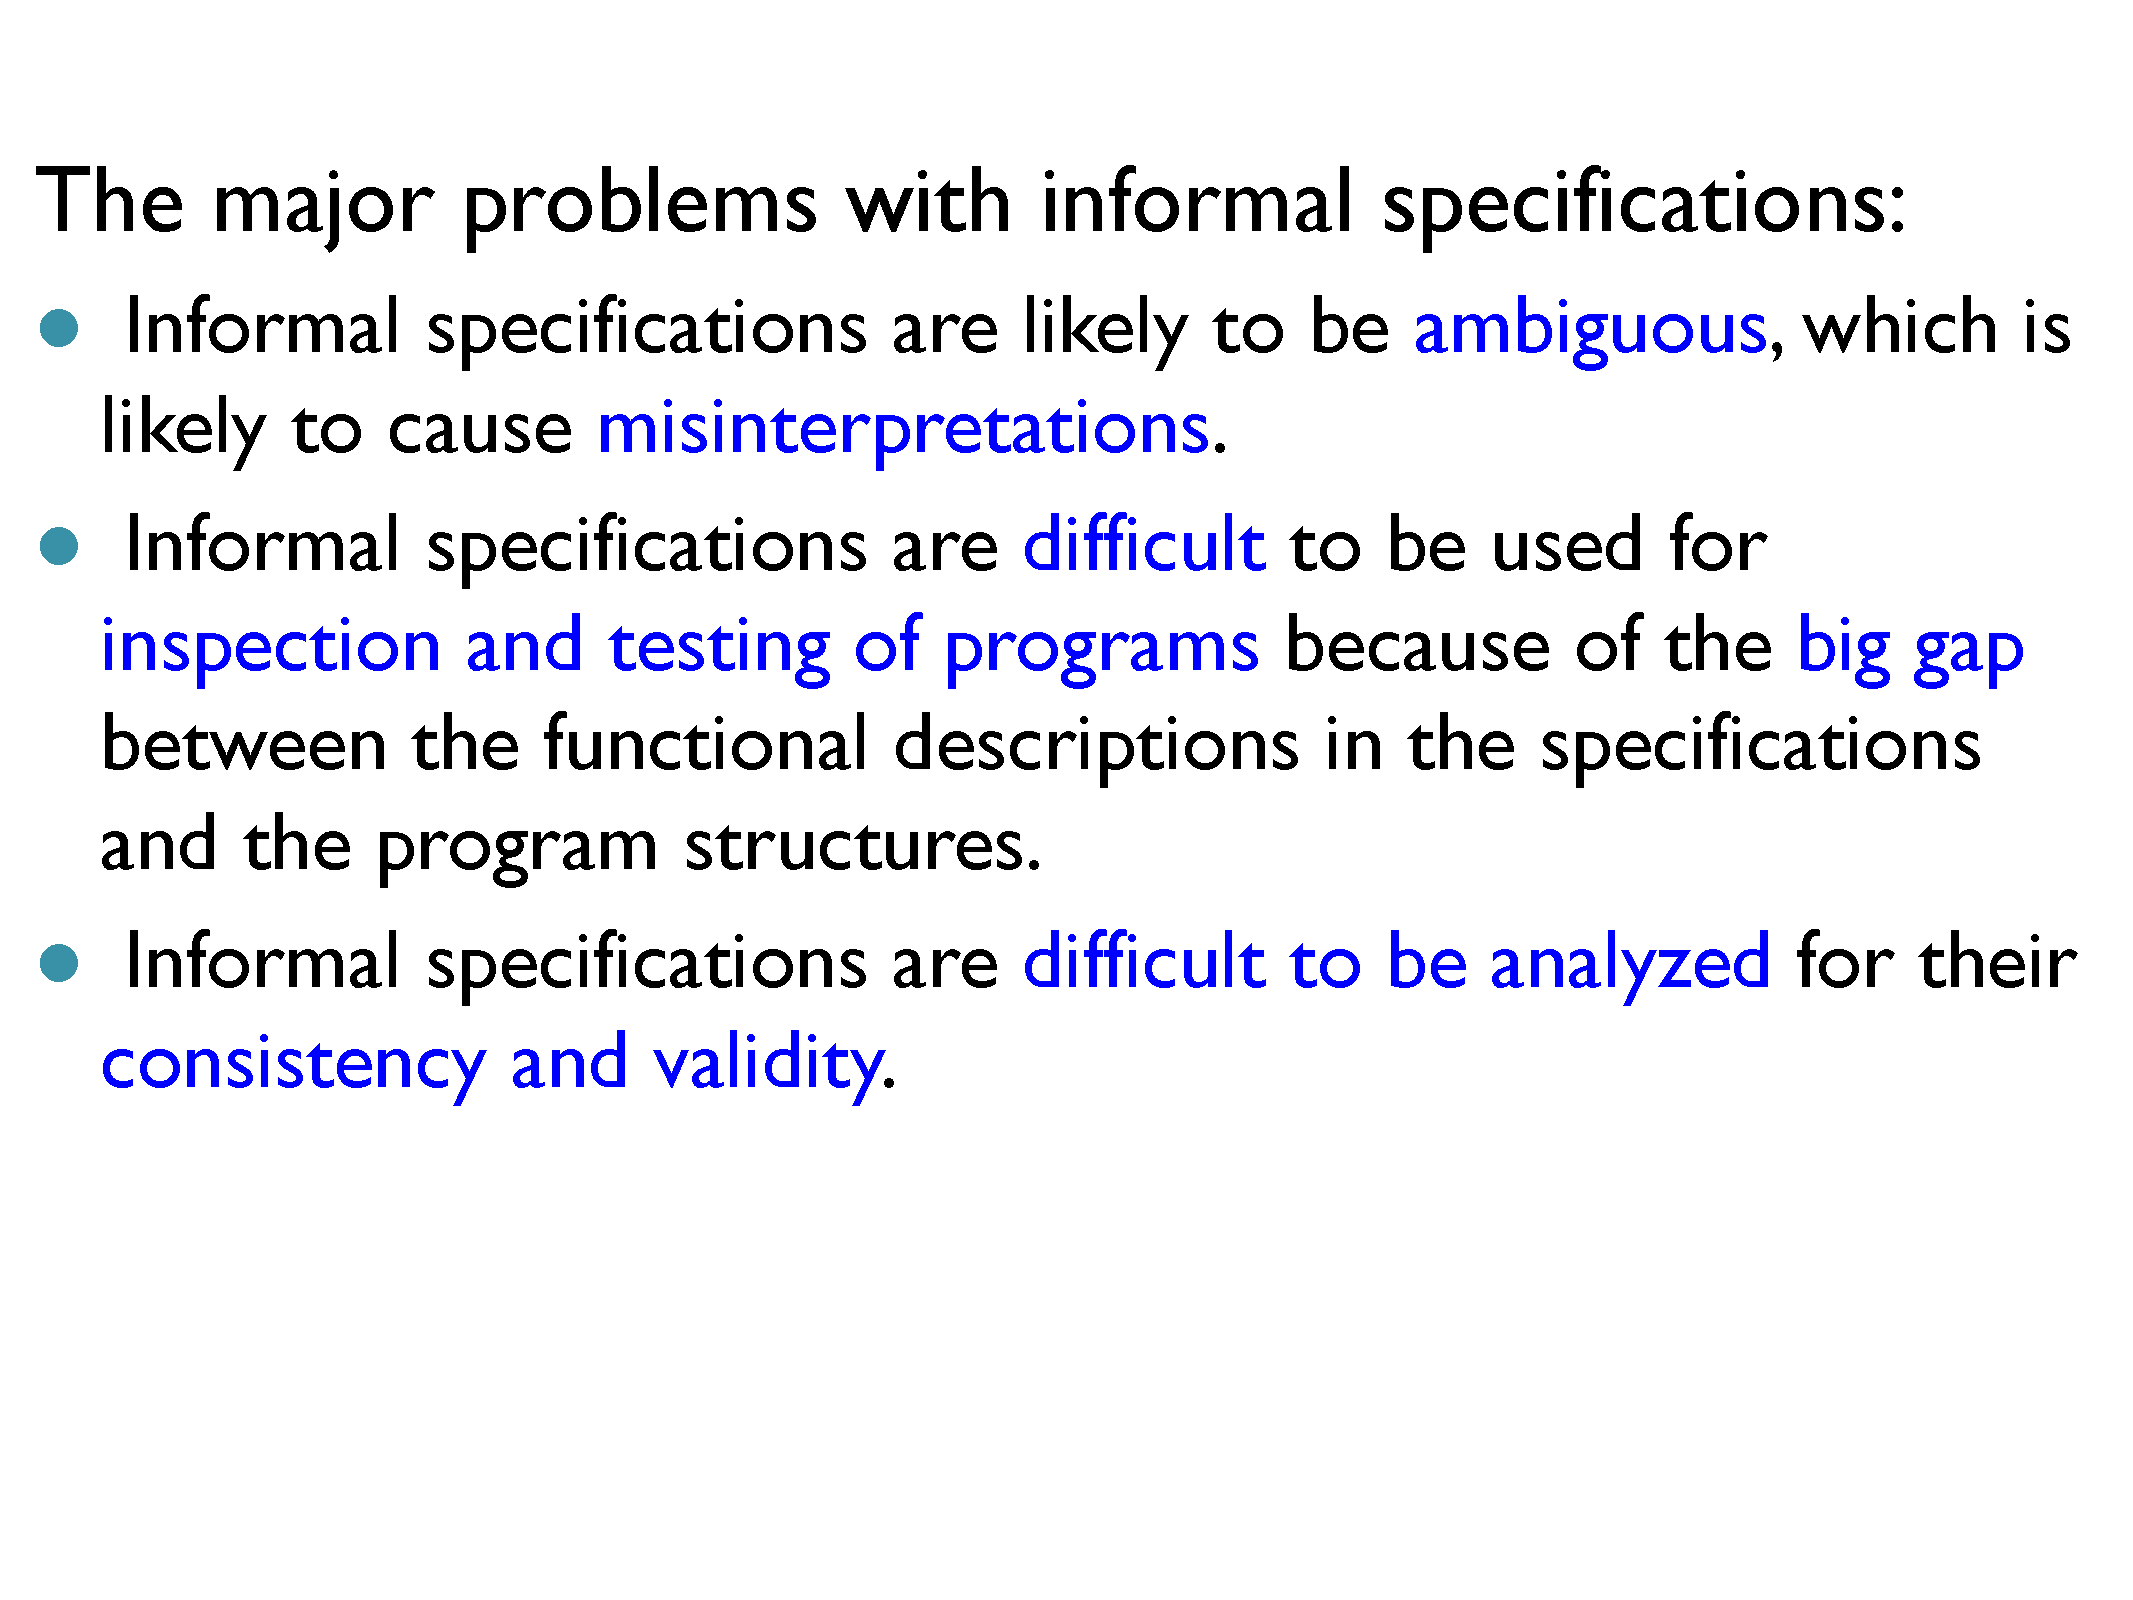
\includegraphics[width=\linewidth]{437.pdf}\\
        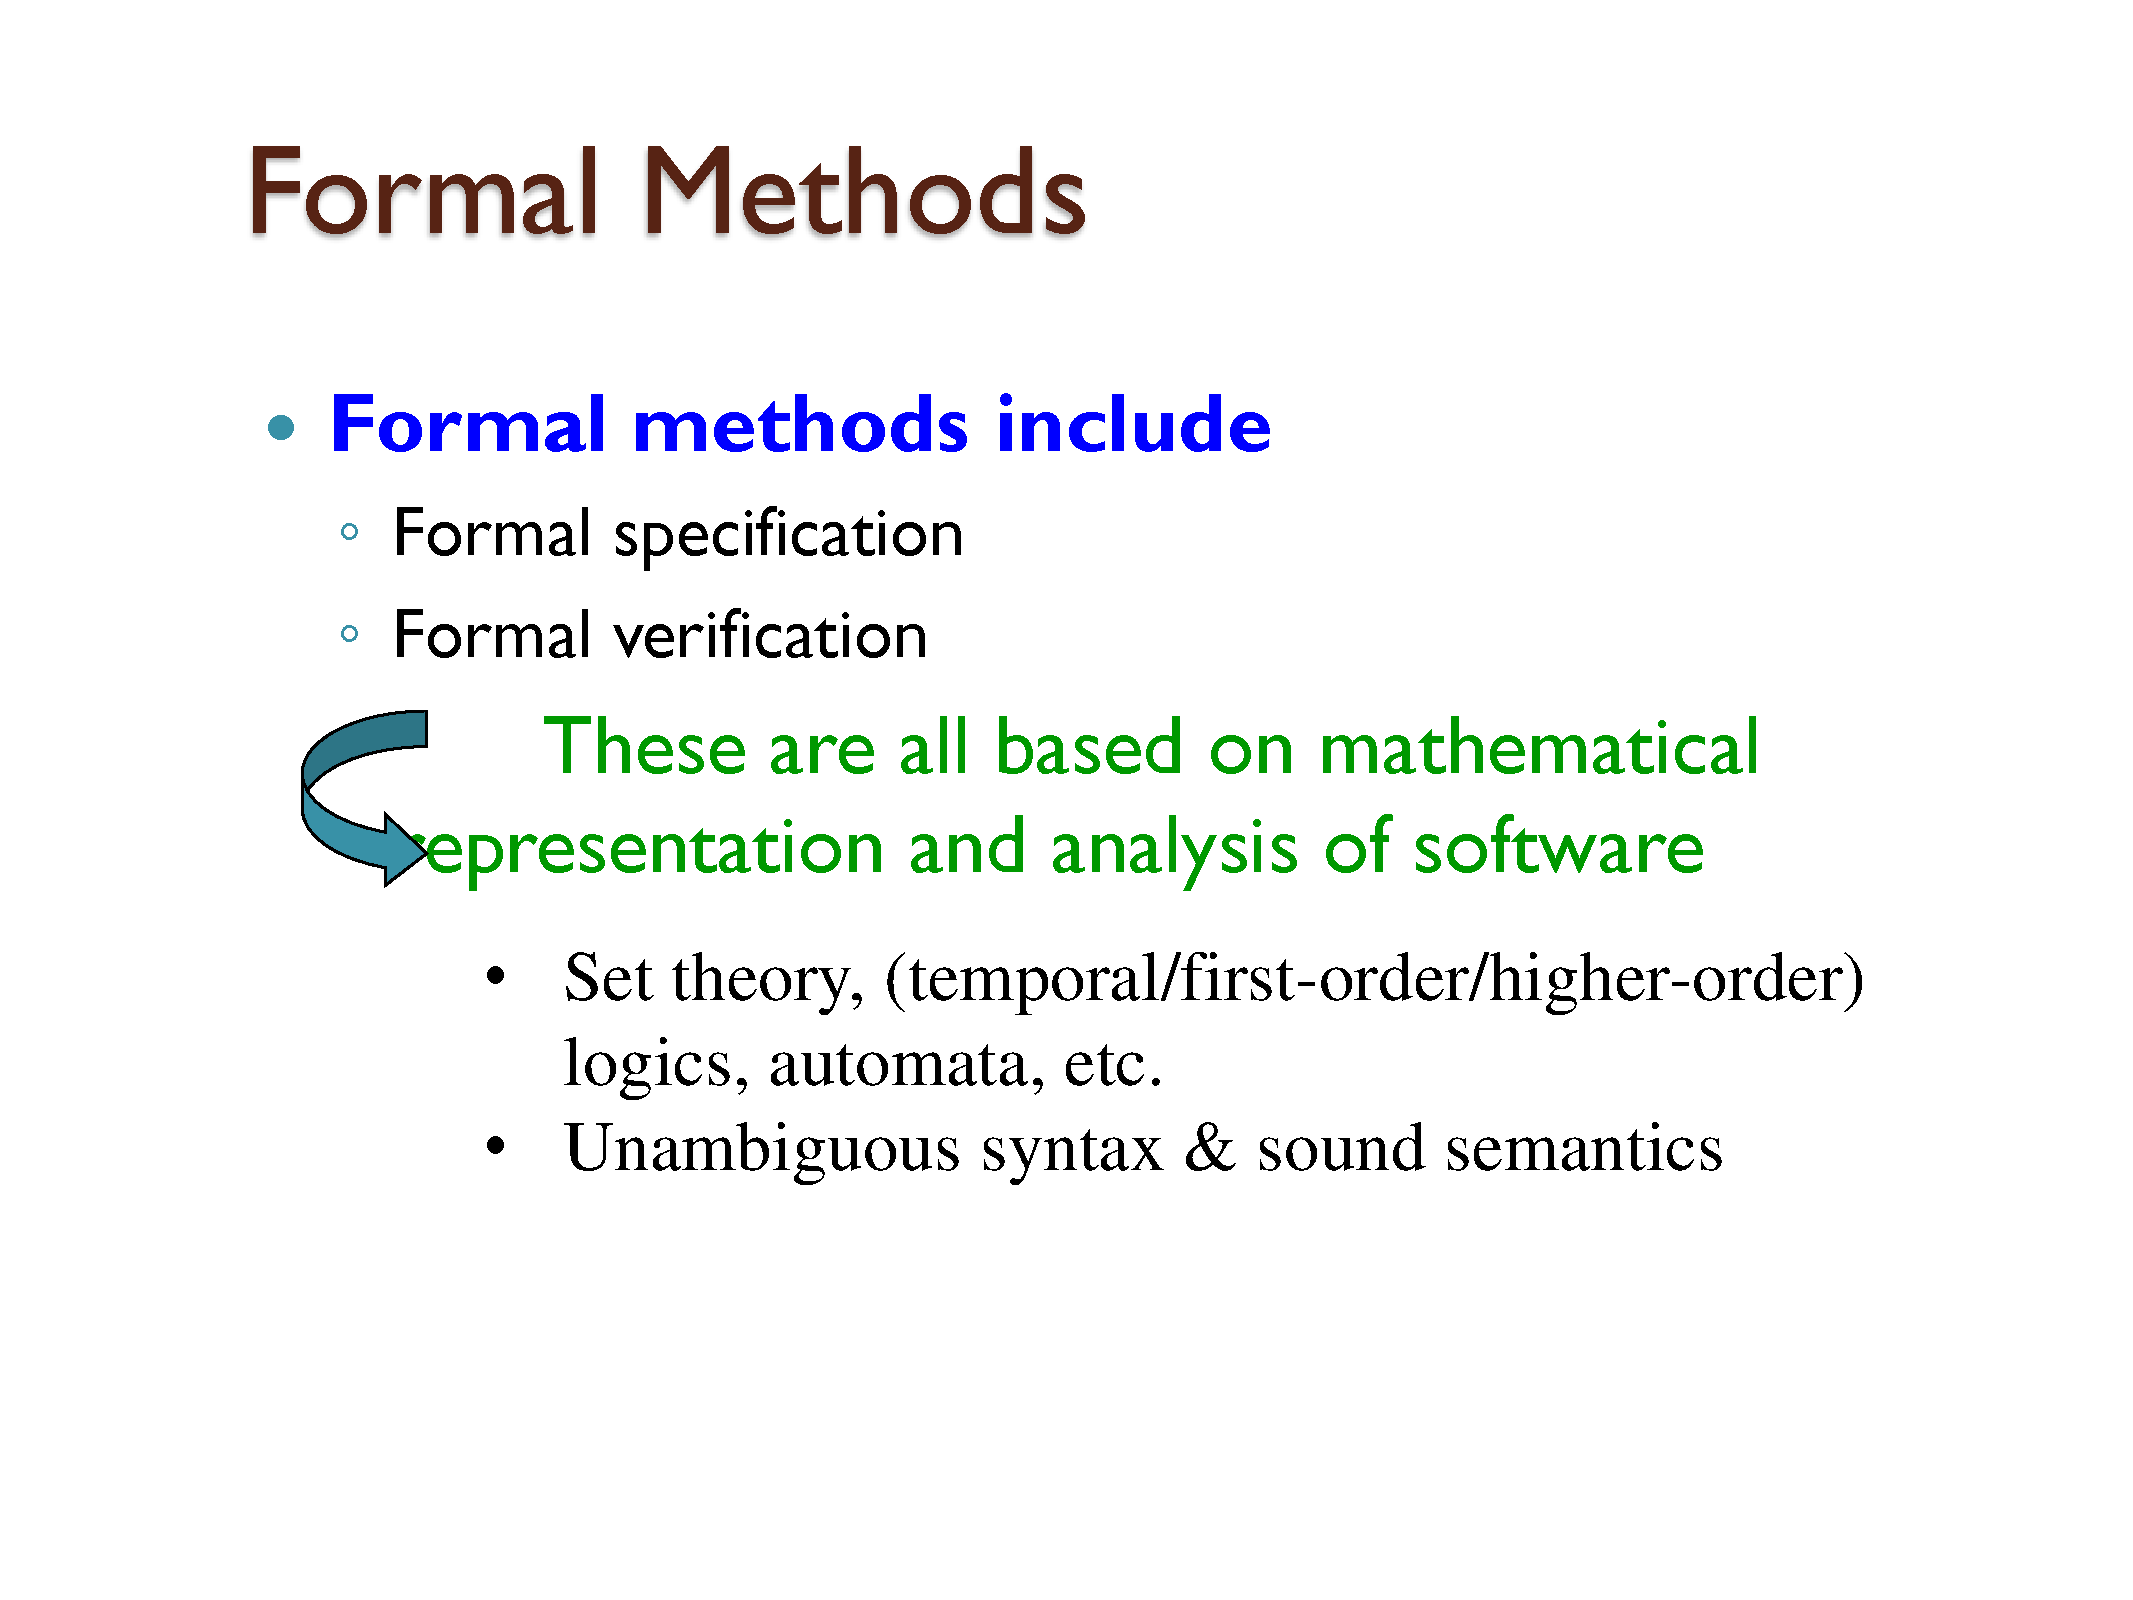
\includegraphics[width=\linewidth]{439.pdf}\\
        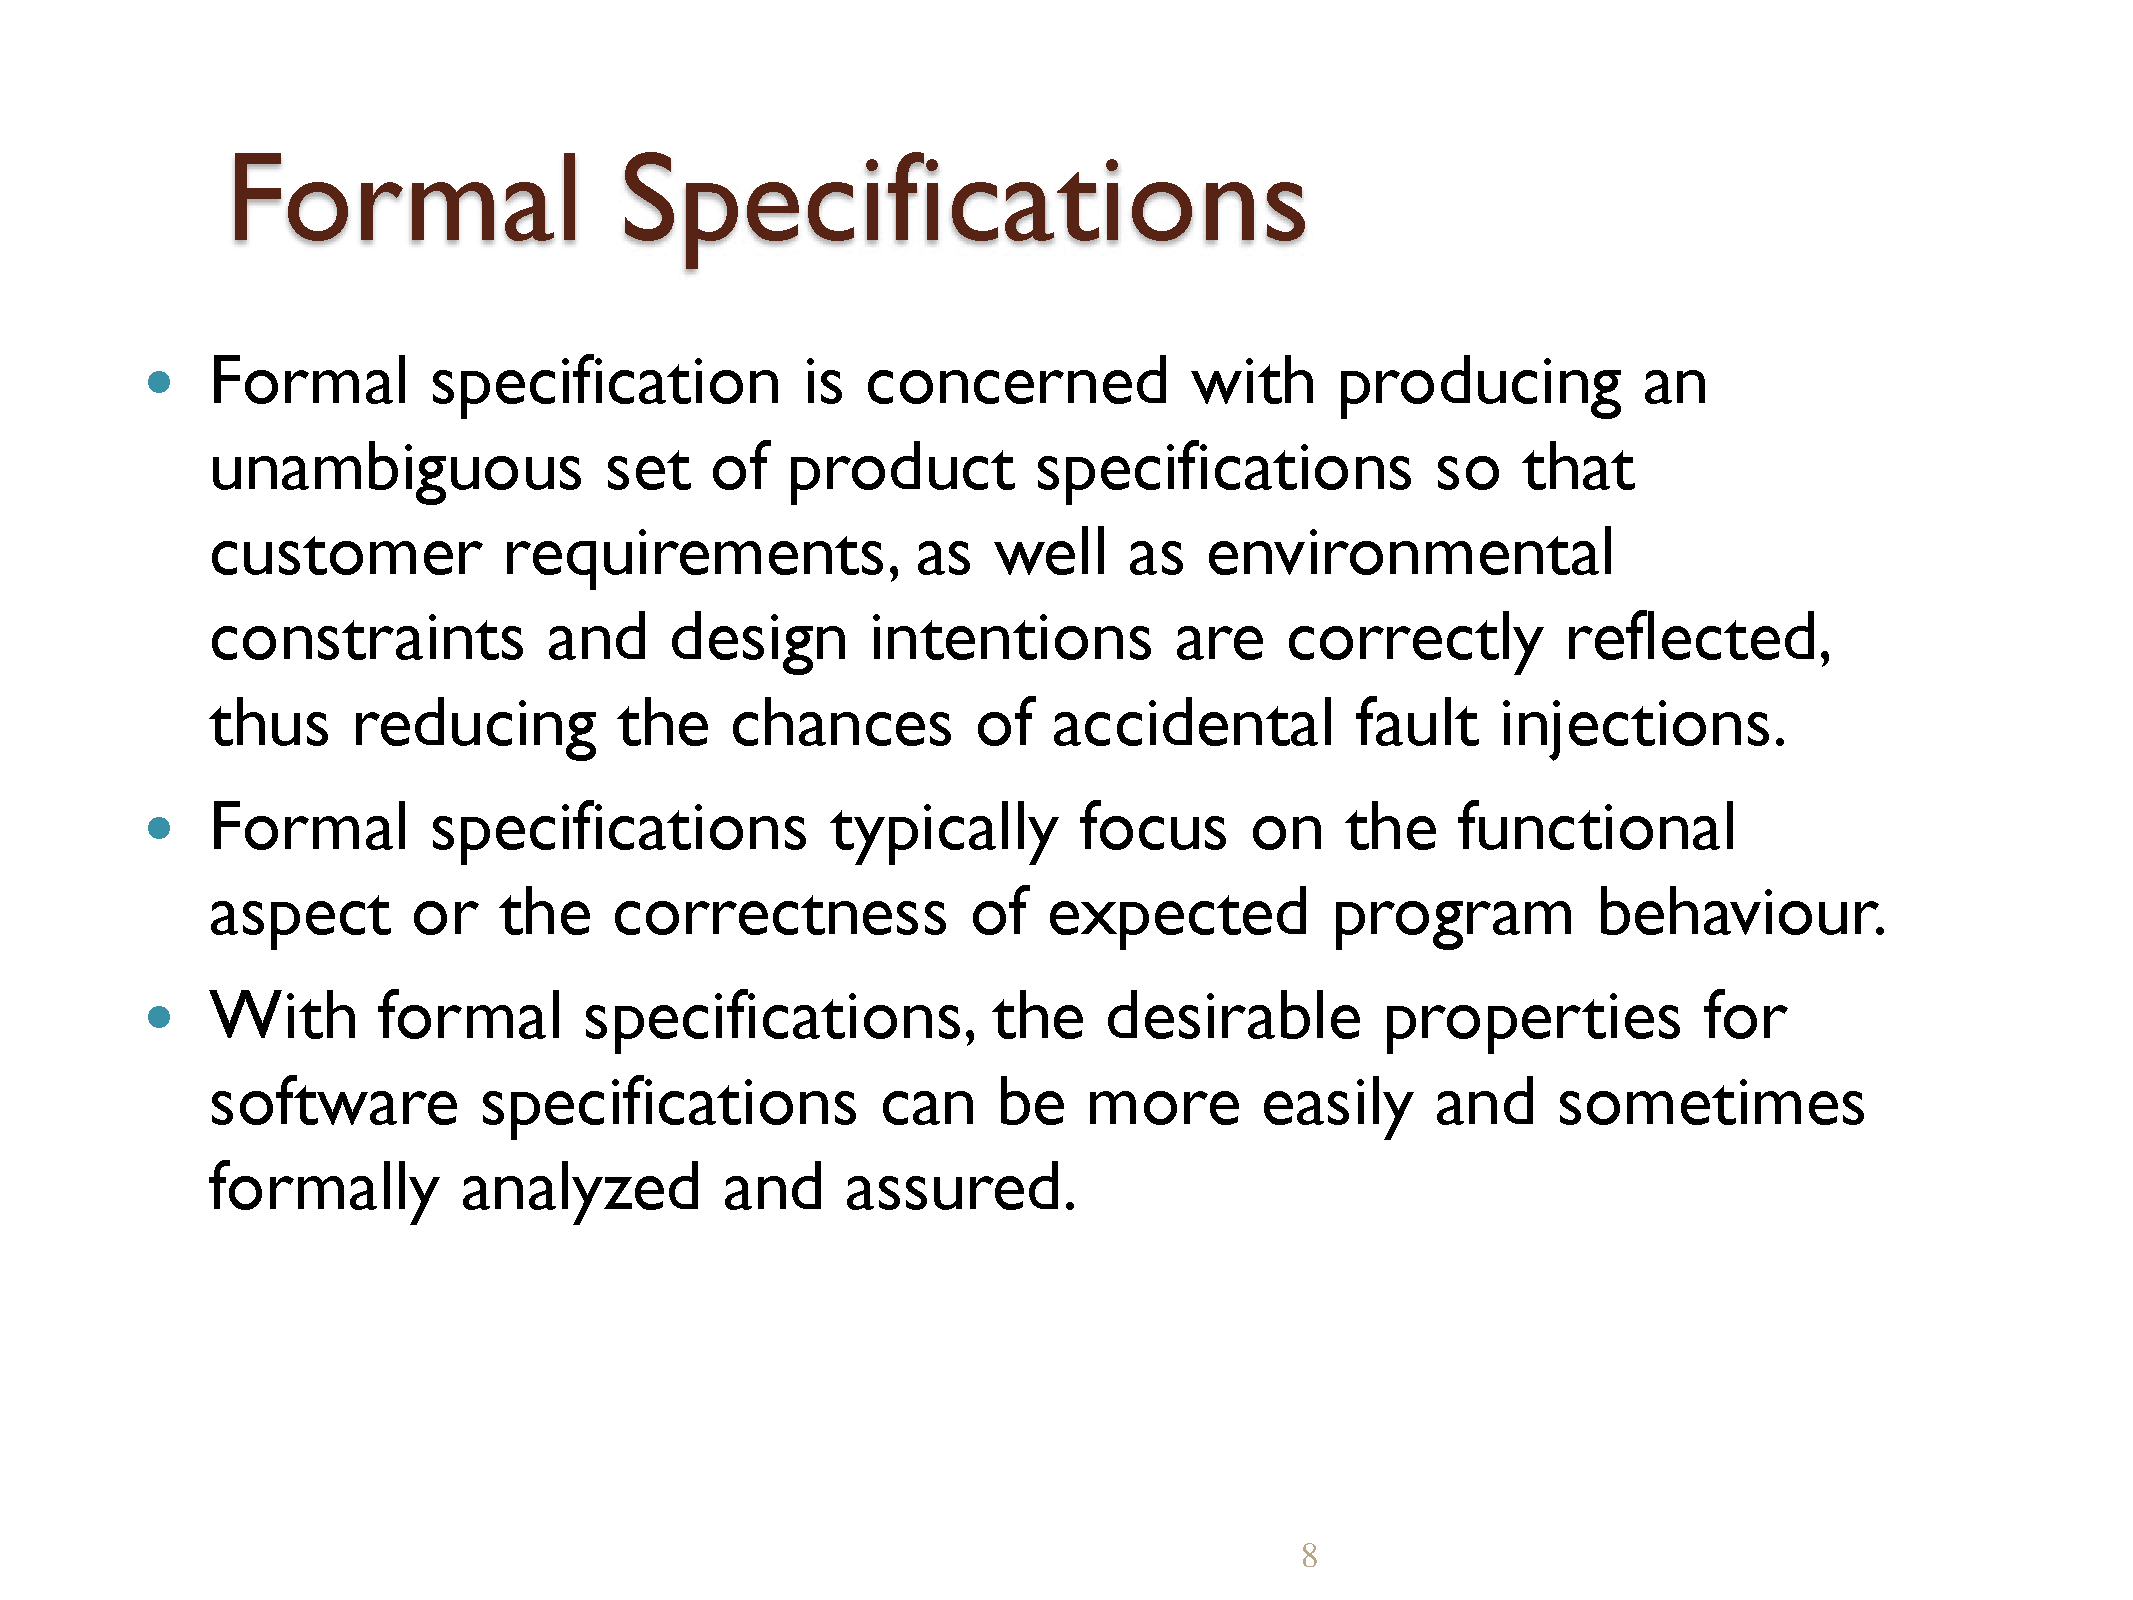
\includegraphics[width=\linewidth]{440.pdf}\\
        \includegraphics[width=\linewidth]{441.pdf}\\
        \includegraphics[width=\linewidth]{442.pdf}\\
        \includegraphics[width=\linewidth]{443.pdf}\\
        \includegraphics[width=\linewidth]{444.pdf}\\
        \includegraphics[width=\linewidth]{448.pdf}\\
        \includegraphics[width=\linewidth]{449.pdf}\\
        \includegraphics[width=\linewidth]{451.pdf}\\
        \includegraphics[width=\linewidth]{452.pdf}\\
        \includegraphics[width=\linewidth]{453.pdf}\\
        \includegraphics[width=\linewidth]{454.png}\\
        \includegraphics[width=\linewidth]{455.pdf}\\
        \includegraphics[width=\linewidth]{456.pdf}\\
        \includegraphics[width=\linewidth]{457.pdf}\\
        \includegraphics[width=\linewidth]{458.pdf}\\
        \includegraphics[width=\linewidth]{459.pdf}\\
        \includegraphics[width=\linewidth]{460.pdf}\\
        \includegraphics[width=\linewidth]{461.pdf}\\
    \end{multicols}
    \end{document}
